\documentclass[a4paper,12pt, twoside]{report}
\usepackage[utf8]{inputenc}
\usepackage[german]{babel}
\usepackage[T1]{fontenc}
\usepackage{lmodern}
\usepackage{amsmath}
\usepackage{amssymb}
\usepackage{amsthm}
\usepackage{geometry}
\usepackage{graphicx}
\usepackage[hidelinks]{hyperref}
\usepackage{listings}
\usepackage{xcolor}
\usepackage{enumitem}
\usepackage{microtype}
\usepackage{booktabs}
\usepackage{array}
\usepackage{rotating}
\usepackage{longtable}

\emergencystretch=4em
\sloppy

% --- 1. \section als oberste Nummerierung einstellen ---
% Entfernt die Kapitelnummer aus der Nummernansicht der Sections (1 statt 0.1)
\renewcommand{\thesection}{\arabic{section}}

% Zähler für Abbildungen, Tabellen und Gleichungen fortlaufend (nicht nach Chapter) nummerieren
\usepackage{chngcntr}
\counterwithout{figure}{chapter}
\counterwithout{table}{chapter}
\counterwithout{equation}{chapter}

% --- 2. Jede \section auf einer neuen rechten Seite beginnen lassen ---
% Falls du \section wie Kapitel behandeln möchtest:
\let\oldsection\section
\renewcommand{\section}{\cleardoublepage\oldsection}

\geometry{margin=2.5cm}

\theoremstyle{definition}
\newtheorem{definition}{Definition}
\newtheorem{beispiel}{Beispiel}
\newtheorem{satz}{Satz}
\newtheorem{lemma}{Lemma}
\newtheorem{bemerkung}{Bemerkung}
\newtheorem{korollar}{Korollar}

\setlist[itemize,1]{label=--}

\sloppy
\emergencystretch=3em

% ---------- Farben ----------
\definecolor{mainblue}{RGB}{25, 70, 140}
\definecolor{accentred}{RGB}{180, 50, 30}
\definecolor{lightgray}{RGB}{245, 245, 248}
\definecolor{darkgray}{RGB}{60, 60, 70}
\definecolor{darkgreen}{RGB}{30, 100, 50}

\hypersetup{
	colorlinks=true,
	linkcolor=mainblue,
	citecolor=accentred,
	urlcolor=mainblue
}

%  Code-Highlighting
\lstset{
	basicstyle=\ttfamily\small,
	keywordstyle=\color{blue},
	commentstyle=\color{gray},
	stringstyle=\color{red},
	numbers=left,
	numberstyle=\tiny,
	breaklines=true,
	breakatwhitespace=false,
	postbreak=\mbox{\textcolor{gray}{$\hookrightarrow$}\space},
	frame=single,
	columns=fullflexible,
	literate=%
	{Ö}{{\"O}}1
	{Ä}{{\"A}}1
	{Ü}{{\"U}}1
	{ß}{{\ss}}1
	{ü}{{\"u}}1
	{ä}{{\"a}}1
	{ö}{{\"o}}1
	{Σ}{{$\Sigma$}}1
	{→}{{$\rightarrow$}}1
	{⊆}{{$\subseteq$}}1
	{⊇}{{$\supseteq$}}1
	{≥}{{$\geq$}}1
}

\title{\textbf{Genomdatenbank und evolutionäre Netzwerkanalyse}}
\author{Stephan Epp}
\date{23. Januar 2026}

\begin{document}

\maketitle

\tableofcontents
\newpage

\section{Einführung}
\label{sec:einleitung}

Biologische Datenbanken enthalten heute Millionen von Netzwerken: metabolische Pfade, Protein-Interaktionsnetzwerke und Gen-Regulationsnetzwerke. Eine zentrale Aufgabe bei der Analyse solcher Datenbanken ist die \emph{Subgraph-Suche}: Gegeben sei ein Query-Netzwerk $G$ (z.\,B. ein bekanntes Motiv wie ein Teilstück der Glykolyse), gesucht sind alle in der Datenbank gespeicherten Netzwerke $G'$, die $G$ als Subgraphen enthalten.

Diese Arbeit beschreibt die konkrete Realisierung einer solchen Suche im System \emph{Gen-DB}, einer Full-Stack-Anwendung bestehend aus einem PostgreSQL-Backend, einer FastAPI-REST-API und einem Web-Frontend. Das System nutzt den \emph{Subgraph Algorithmus} \cite{epp2026subgraph} mit Laufzeit $O(n^3)$ zur strukturellen Analyse biologischer Netzwerke, dargestellt als Adjazenzmatrizen. Über diese Einzelaufgabe hinaus zeigt die Arbeit, dass sich der Vergleichskern von der Art der biologischen Daten trennen lässt: Jede endliche attributierte relationale Struktur wird verlustfrei in einen Stapel von Mengenfolgen kodiert, auf dem Vergleich und invertierter Index nachweislich korrekt und bis auf einen konstanten Faktor optimal sind (Abschnitt~\ref{sec:universell}).

\subsection{Beitrag dieser Arbeit}

\begin{itemize}
	\item Formale Beschreibung der Systemarchitektur von Gen-DB und Einbettung des Subgraph Algorithmus in eine relationale Datenbank.
	\item Formaler Nachweis der Korrektheit und Komplexität des Such-Pipeline-Prozesses (Pre-Filtering $+$ Subgraph-Vergleich).
	\item Empirische Evaluation an einer synthetisch generierten Datenbank mit $1.000.000$ biologischen Netzwerken.
	\item Veranschaulichung der Ergebnisse durch matplotlib-Diagramme: Laufzeitverteilung, Pre-Filter-Effektivität, Skalierungsverhalten und Trefferverteilung.
	\item Experimenteller Vergleich des Subgraph Algorithmus mit VF2 sowie Analyse der Ursachen der beobachteten Laufzeitunterschiede.
	\item Experimentelle Untersuchung der parallelen Ausführung der Kandidatenvergleiche mit $1$, $2$ und $3$ Worker-Prozessen (Gesamtzeit, Speedup, Effizienz, Skalierung mit der Kandidatenzahl).
	\item Experimenteller Vergleich der Python- und C++-Implementierung des Subgraph Algorithmus über eine direkt im Worker-Prozess aufgerufene C++-Library, einschließlich Mikrobenchmark, Ende-zu-Ende-Suchmessung, Trefferabgleich und Analyse der verbleibenden Schnittstellenkosten.
	\item Erweiterung des Suchmodells auf geschichtete Multi-Omics-Netzwerke und experimentelle Prüfung der kohärenten und unabhängigen Schichtrelationen mit Python- und C++-Backends, synthetischer Ground Truth, Mikrobenchmark und Ende-zu-Ende-Messung.
	\item Universelle Kodierung biologischer Strukturen und optimale Suche (Abschnitt~\ref{sec:universell}): Der Vergleichskern wird auf Stapel von Mengenfolgen (\emph{Schichten} und \emph{Komponenten}) beschränkt und von der Art der Daten getrennt. Formal gezeigt werden
	\begin{itemize}
		\item die Definition der Relationen $\sqsubseteq_{\mathrm{ind}}$ (unabhängig je Schicht) und $\sqsubseteq_{\mathrm{coh}}$ (kohärent über alle Schichten) samt ihrer elementaren Eigenschaften, darunter die Nicht-Transitivität und das Fehlen eines zulässigen Kantenzahl-Filters (Lemmata~\ref{lem:univ_eigenschaften} und \ref{lem:univ_kanten});
		\item die Definition von Schema, Struktur, Koordinatensystem und Kodierung $\Phi_{\Sigma,\kappa}$ für gerichtete, ungerichtete, gewichtete und attributierte Netzwerke, mehrstellige Reaktionen, Hypergraphen, Pfade, Ontologien und mehrschichtige Netzwerke, die Verlustfreiheit der Kodierung (Satz~\ref{satz:univ_verlustfrei}) und ihr Aufwand von $O(|S|\log|S|)$ (Satz~\ref{satz:univ_kodierung_zeit});
		\item der Vergleich zweier Stapel in erwarteter Linearzeit (Satz~\ref{satz:univ_vergleich}) mit passender unterer Schranke $\Omega(m+m')$ (Satz~\ref{satz:univ_untere}), also bis auf einen konstanten Faktor optimal;
		\item ein invertierter Paarindex, dessen Suche das exakte Ergebnis ohne Einzelvergleiche liefert und dessen Aufwand von der Trefferlast und nicht von der Datenbankgröße $N$ abhängt (Sätze~\ref{satz:univ_index} und \ref{satz:univ_index_zeit}, Korollar~\ref{kor:univ_unabhaengig});
		\item die Kernunabhängigkeit (Korollar~\ref{kor:univ_kern}): Für eine neue biologische Struktur genügt ein neues Schema; Vergleich, Index und Beweise bleiben unverändert;
		\item die ausdrücklichen Grenzen der Aussagen: die Optimalität gilt für die definierte Relation und nicht für die klassische Subgraph-Isomorphie (Bemerkung~\ref{bem:univ_np}), und die fachliche Validität einer Kodierung ist nicht mitbewiesen (Bemerkung~\ref{bem:univ_semantik}); zudem die Vorbereitung der Umsetzung in Python.
	\end{itemize}
	\item Zusammenfassung, kritische Würdigung der Grenzen und ausführlicher, nach Themenfeldern geordneter Ausblick auf Erweiterungen (Korrektheit, Indexierung, Beschleunigung der Vergleiche, Systemebene, Evaluation, Anwendung, Kopplung und Schnittstellen, Multi-Omics-Suche sowie Umsetzung, Messung und Erweiterung der universellen Kodierung) mit einer Priorisierung der nächsten Schritte.
\end{itemize}

\subsection{Aufbau der Arbeit}

Die Arbeit gliedert sich in aufeinander aufbauende Abschnitte: von den theoretischen Grundlagen über das System und seine formale Analyse und die Experimente bis zu einer verallgemeinernden Theorie der universellen Kodierung und dem Ausblick.

Abschnitt~\ref{sec:grundlagen} führt in biologische Netzwerke, ihre Adjazenzmatrix-Repräsentation, die Spaltensignaturen und den Subgraph Algorithmus ein, dessen Laufzeit von $O(n^3)$ die Grundlage aller späteren Betrachtungen ist. Abschnitt~\ref{sec:architektur} beschreibt die Systemarchitektur und das Datenmodell von Gen-DB und erläutert anhand von UML-Paket- und Klassendiagrammen den Aufbau der Anwendung. Abschnitt~\ref{sec:pipeline} formalisiert die Such-Pipeline, insbesondere die Vorauswahl anhand von Knoten- und Kantenzahl, und untersucht deren Korrektheit und Laufzeitkomplexität; ein Serverprotokoll veranschaulicht dort zusätzlich den Ablauf einer konkreten Suche.

Der zweite Teil der Arbeit ist empirisch. Abschnitt~\ref{sec:evaluation} stellt den Versuchsaufbau sowie die Ergebnisse zur generierten Datenbank mit einer Million Netzwerken und zum Verhalten der Vorauswahl vor und schließt mit einer Diskussion. Abschnitt~\ref{sec:vergleich} widmet sich dem experimentellen Vergleich mit etablierten Verfahren, analysiert die beobachteten Laufzeitunterschiede und ordnet die Verfahren in die Fachliteratur ein. Abschnitt~\ref{sec:parallel} untersucht anschließend, wie sich die gesamte Suche verhält, wenn die Kandidatenvergleiche auf mehrere Prozesse verteilt werden. Er beschreibt die Implementierung der parallelen Ausführung, ein reproduzierbares Experiment mit einem, zwei und drei Worker-Prozessen und die Auswertung nach Gesamtzeit, Speedup, Effizienz und Skalierung mit der Kandidatenzahl. Abschnitt~\ref{sec:backends} vergleicht darauf aufbauend die Python- und C++-Implementierungen. Die C++-Variante wird dabei als Library direkt im Worker-Prozess aufgerufen; Mikrobenchmark und Ende-zu-Ende-Messung trennen so den Aufwand des Algorithmuskerns von den Kosten der Sprachschnittstelle. Abschnitt~\ref{sec:multiomics} erweitert diese Untersuchungen auf geschichtete Multi-Omics-Netzwerke: Er definiert kohärente und unabhängige Schichtvergleiche, dokumentiert den synthetischen Versuchsaufbau mit bekannter Ground Truth und wertet die abgeschlossenen Korrektheits-, Mikrobenchmark-, Ende-zu-Ende-, Worker- und Chunk-Experimente aus. Die abgebrochene Datenbankgrößenreihe wird als unvollständig eingeordnet. Der letzte Unterabschnitt (Abschnitt~\ref{sec:fremde_beschreibungen}) ordnet die Messergebnisse in die Frage ein, wie lose Kopplung und klare Beschreibungsgrenzen in Gen-DB zusammenwirken.

Nach den Experimenten kehrt die Arbeit in Abschnitt~\ref{sec:universell} zur Theorie zurück und verallgemeinert die bisherige Vorgehensweise. Bisher wurde für jede neue Art biologischer Daten ein eigener Vergleichspfad formuliert und im nativen Kern umgesetzt: zuerst für das Einzelnetzwerk (Abschnitt~\ref{sec:pipeline}), dann für das mehrschichtige Netzwerk (Abschnitt~\ref{sec:multiomics}). Der neue Abschnitt trennt die Suche in einen strukturunabhängigen Kern, der nur Stapel von Mengenfolgen kennt, und eine Kodierung, die jede biologische Struktur eines beliebigen Schemas in einen solchen Stapel überführt. Er besteht aus sieben Unterabschnitten:
\begin{itemize}
	\item Der \emph{strukturunabhängige Kern} (Abschnitt~\ref{sec:univ_kern}) definiert Schichten, Stapel, Paarmengen und die beiden Enthaltenseinsrelationen $\sqsubseteq_{\mathrm{ind}}$ und $\sqsubseteq_{\mathrm{coh}}$, zeigt den Matrixstapel als Spezialfall der bisherigen Multi-Omics-Relation und beweist ihre elementaren Eigenschaften, darunter die fehlende Transitivität und die Unzulässigkeit des Kantenzahl-Filters.
	\item Der Unterabschnitt \emph{Biologische Strukturen und ihre Kodierung} (Abschnitt~\ref{sec:univ_kodierung}) führt Schema, Struktur, Koordinatensystem und die Kodierung $\Phi_{\Sigma,\kappa}$ ein, belegt sie an einem Beispiel mit einem regulatorischen Netzwerk und einer dreistelligen Reaktion und beweist Verlustfreiheit und fast linearen Aufwand. Bemerkungen zu lokalen und globalen Koordinaten sowie zur Schemaänderung ergänzen ihn.
	\item Der \emph{optimale Vergleich zweier Stapel} (Abschnitt~\ref{sec:univ_vergleich}) beweist eine obere Schranke in erwarteter Linearzeit und eine untere Schranke durch ein Gegenspielerargument, sodass der Vergleich bis auf einen konstanten Faktor optimal ist.
	\item Der \emph{invertierte Index} (Abschnitt~\ref{sec:univ_index}) definiert den Paarindex und das Suchergebnis, beweist die Korrektheit der Suche ohne Einzelvergleiche und ihre Laufzeit in Abhängigkeit von der Trefferlast, folgert die Unabhängigkeit von $N$ unter einer Häufigkeitsannahme, behandelt die umgekehrte Suchrichtung und setzt den Index in Beziehung zur bisherigen Pipeline.
	\item \emph{Kernunabhängigkeit und Reichweite} (Abschnitt~\ref{sec:univ_reichweite}) hält fest, dass alle Sätze für jedes Schema gelten, ordnet die native C++-Bibliothek als optionalen Beschleuniger ein und benennt die Grenzen: die NP-Vollständigkeit des klassischen Teilgraph-Isomorphieproblems und die offene fachliche Semantik.
	\item Die \emph{Vorbereitung des zweiten Schritts} (Abschnitt~\ref{sec:univ_umsetzung}) beschreibt die Umsetzung in Python: Schnittstelle je Strukturart, Entitätsregister, Indextabelle, die aus den Sätzen folgenden Tests und das noch ausstehende Experiment.
	\item Eine kurze \emph{Zusammenfassung} schließt den Abschnitt.
\end{itemize}
Der Abschnitt enthält ausschließlich formale Aussagen und keine Messungen; die Laufzeitaussagen sind Folgerungen aus den Sätzen und im zweiten Schritt experimentell zu prüfen.

Das abschließende Kapitel „Schluss“ (Abschnitt~\ref{sec:schluss}) besteht aus fünf Teilen. Es fasst die Ergebnisse aller Abschnitte zusammen, einschließlich der universellen Kodierung (Abschnitt~\ref{sec:zusammenfassung}, dort insbesondere Abschnitt~\ref{sec:zus_universell}), benennt die Grenzen der Arbeit (Abschnitt~\ref{sec:grenzen}), entwickelt einen ausführlichen, nach neun Themenfeldern A bis I geordneten Ausblick mit möglichen Erweiterungen und offenen Forschungsfragen, von denen das Themenfeld I die Umsetzung, Messung und Erweiterung der universellen Kodierung behandelt (Abschnitt~\ref{sec:ausblick}), schlägt eine Reihenfolge für die nächsten Entwicklungsschritte vor (Abschnitt~\ref{sec:prio}) und schließt mit einer Gesamteinschätzung (Abschnitt~\ref{sec:schlussbemerkung}).

\section{Grundlagen}
\label{sec:grundlagen}

\subsection{Graphen und Adjazenzmatrizen}

\begin{definition}[Biologisches Netzwerk]
	Ein biologisches Netzwerk ist ein gerichteter Graph $G = (V, E)$ mit Knotenmenge $V = \{v_1, \ldots, v_n\}$ (Metabolite, Proteine oder Gene) und Kantenmenge $E \subseteq V \times V$ (Reaktionen, Interaktionen oder Regulationsbeziehungen). Jedem Knoten $v_i$ ist ein Label $\ell(v_i) \in \Sigma_{\text{Bio}}$ aus einem biologischen Vokabular zugeordnet.
\end{definition}

\begin{definition}[Adjazenzmatrix-Repräsentation]
	Ein Netzwerk $G$ mit $n$ Knoten wird in Gen-DB als Tupel
	\[
	G = (L, A) \quad \text{mit } L \in \Sigma_{\text{Bio}}^n,\ A \in \{0,1\}^{n \times n}
	\]
	gespeichert, wobei $L$ der Vektor der Knotenlabels und $A$ die Adjazenzmatrix mit $A_{ij} = 1 \Leftrightarrow (v_i, v_j) \in E$ ist.
\end{definition}

\subsection{Signaturen und Subgraph-Relation}

\begin{definition}[Spaltensignatur]
	Für eine Adjazenzmatrix $A \in \{0,1\}^{n \times n}$ ist die Signatur der Spalte $j$ definiert als
	\[
	\sigma_j(A) = \sum_{i=0}^{n-1} A_{ij} \cdot 2^i + j \cdot 2^n.
	\]
\end{definition}

\begin{definition}[Signatur-Array und Hash]
	Das Signatur-Array von $A$ ist $\Sigma(A) = (\sigma_0(A), \ldots, \sigma_{n-1}(A))$. Der Signatur-Hash ist
	\[
	h(A) = \mathrm{SHA256}\bigl(\mathrm{str}(\Sigma(A))\bigr).
	\]
\end{definition}

\begin{lemma}[Injektivität der Signaturfunktion]
	\label{lem:injektiv}
	Die Abbildung $\sigma: \{0,1\}^n \times \{0,\ldots,n-1\} \to \mathbb{N}$, $(c, j) \mapsto \sum_{i=0}^{n-1} c_i 2^i + j2^n$ ist injektiv.
\end{lemma}

\begin{proof}
	Sei $\sigma(c,j) = \sigma(c',j')$. Da $\sum_{i=0}^{n-1} c_i 2^i \in [0, 2^n-1]$ und $j2^n, j'2^n$ Vielfache von $2^n$ sind, folgt aus der Eindeutigkeit der Division mit Rest (Divisionsalgorithmus für $2^n$), dass $j = j'$ und somit $\sum c_i 2^i = \sum c_i' 2^i$. Da die Binärdarstellung eindeutig ist, folgt $c = c'$.
\end{proof}

\begin{definition}[Subgraph-Relation, zyklisch]
	Für Adjazenzmatrizen $A \in \{0,1\}^{n_A \times n_A}$ und $B \in \{0,1\}^{n_B \times n_B}$ mit $n_A \le n_B$ schreiben wir $A \preceq B$ (``$A$ ist zyklischer Subgraph von $B$''), wenn es eine zyklische Rotation $r \in \{0,\ldots,n_B-1\}$ und eine Startposition $s$ gibt, sodass die Zeilenkomponenten der Signaturen von $A$ als längste gemeinsame Teilsequenz (LCS) der Länge $\geq 2$ in der rotierten Zeilenkomponentensequenz von $B$ ab Position $s$ auftreten.
\end{definition}

\subsection{Der Subgraph Algorithmus}

Der Subgraph Algorithmus \cite{epp2026subgraph} berechnet für zwei Matrizen $A, B$ in drei Schritten, ob $A \preceq B$, $B \preceq A$, beide äquivalent oder unvergleichbar sind:

\begin{enumerate}
	\item Berechne $\Sigma(A)$ und $\Sigma(B)$ — Aufwand $O(n_A^2 + n_B^2)$.
	\item Extrahiere Zeilenkomponenten $\rho(A) = (\sigma_j(A) \bmod 2^{n_A})_j$, analog für $B$.
	\item Für jede der $n_B$ zyklischen Rotationen von $\rho(B)$: Vergleiche mit $\rho(A)$ via LCS in $O(n_A \cdot n_B)$.
\end{enumerate}

\begin{satz}[Laufzeit des Subgraph Algorithmus]
	\label{satz:laufzeit}
	Für $n = \max(n_A, n_B)$ benötigt der Subgraph Algorithmus $O(n^3)$ Zeit.
\end{satz}

\begin{proof}
	Schritt 1 ist $O(n^2)$. Schritt 3 besteht aus $n_B \le n$ Rotationen, jede mit LCS-Vergleich in $O(n_A n_B) \subseteq O(n^2)$, insgesamt $O(n^3)$. Schritt 2 ist $O(n)$. Die Summe ist $O(n^2) + O(n) + O(n^3) = O(n^3)$.
\end{proof}

Eine vollständige Optimalitätsanalyse $\Omega(n^{3-\varepsilon})$ unter SETH findet sich in \cite{epp2026subgraph}; sie wird hier als gegeben vorausgesetzt und in Abschnitt~\ref{sec:pipeline} auf den Datenbankkontext übertragen.

\section{Systemarchitektur von Gen-DB}
\label{sec:architektur}

\subsection{Komponentenübersicht}

Gen-DB besteht aus drei Schichten:

\begin{itemize}
	\item \textbf{Frontend} (HTML/CSS/JavaScript): Erstellung, Anzeige und Suche von Netzwerken über REST-Aufrufe.
	\item \textbf{Backend} (FastAPI, Python): REST-Endpunkte \texttt{/api/networks}, \texttt{/api/networks/\{id\}}, \texttt{/api/networks/search}; Modul \texttt{crud.py} implementiert Signaturberechnung und ruft den Subgraph Algorithmus auf.
	\item \textbf{Datenbank} (PostgreSQL): Tabellen \texttt{biological\_networks} (Metadaten: Name, Typ, Organismus, Knoten-/Kantenzahl) und \texttt{network\_matrices} (Knotenlabels, Adjazenzmatrix, Signatur-Array, Signatur-Hash).
\end{itemize}

\begin{definition}[Datenbankzustand]
	Der Datenbankzustand zum Zeitpunkt $t$ ist eine endliche Menge
	\[
	\mathcal{D}_t = \{(id_k, L_k, A_k, \Sigma_k, h_k) : k = 1,\ldots,N_t\},
	\]
	wobei $N_t = |\mathcal{D}_t|$ die Anzahl gespeicherter Netzwerke ist. In der vorliegenden Evaluation gilt $N_t \approx 1.000.002$.
\end{definition}

\subsection{Datenmodell}

Die Speicherung erfolgt normalisiert über zwei $1{:}1$-verknüpfte Relationen:

\[
\texttt{biological\_networks}(\underline{\text{network\_id}}, \text{name}, \text{type}, \text{organism}, \text{node\_count}, \text{edge\_count})
\]
\[
\texttt{network\_matrices}(\underline{\text{network\_id}}, L, A, \Sigma, h)
\]

Die Spalten \texttt{node\_count} und \texttt{edge\_count} entsprechen $n_k = |V_k|$ bzw. $m_k = |E_k| = \sum_{i,j} (A_k)_{ij}$ und werden für das Pre-Filtering (Abschnitt~\ref{sec:prefilter}) materialisiert, um eine vollständige Tabellenabtastung zu vermeiden.

\subsection{UML-Architekturmodelle von Gen-DB}
\label{sec:uml}

Die beiden UML-Diagramme in den Abbildungen~\ref{fig:uml-packages} und~\ref{fig:uml-classes} dokumentieren die Struktur von Gen-DB auf Paket- und Klassenebene und bilden damit die konzeptionelle Grundlage für die in den folgenden Abschnitten formalisierten Such- und Datenbankprozesse.

Das Paketdiagramm zeigt die fachliche und technische Zerlegung der Anwendung in drei logisch getrennte Bausteine: das Web-Frontend, das Backend mit den API- und Suchkomponenten und die persistente Datenspeicherung in PostgreSQL. Dieser Aufbau ist keine rein dokumentarische Anordnung, sondern entspricht einem klaren Entwurfsmuster für skalierbare Datenbankanwendungen: Die Präsentationsschicht übernimmt keine Datenlogik, sondern stellt lediglich die Interaktion mit dem Benutzer bereit; die Logikschicht kapselt die Kernfunktionalität der Signaturberechnung, des Pre-Filters und des Subgraph-Checks; die Datenbankschicht speichert neben den Netzwerkinhalten auch die maschinenlesbaren Repräsentationen, die für die Suche benötigt werden. Aus Sicht der Systemarchitektur ist deshalb besonders wichtig, dass die Datenflussrichtung zwischen den Schichten eindeutig ist: Ein Nutzer erzeugt oder lädt ein biologisches Netzwerk über das Frontend; die Anfrage wird als API-Request an das Backend weitergeleitet; dort werden Netzwerkdaten interpretiert, normalisiert und in Form von Knotenlabels und Adjazenzmatrizen für den Subgraph Algorithmus aufbereitet; danach werden die passenden Kandidaten mit SQL-Filterkriterien aus der Datenbank abgerufen und im Ergebnis an die Präsentationsschicht zurückgegeben. Das Paketdiagramm macht damit sichtbar, dass Gen-DB als System nicht nur aus einer einzelnen Anwendung besteht, sondern aus einer zusammengesetzten, modularen Architektur, in der fachliche Trennung und technische Verantwortlichkeit klar voneinander abgegrenzt sind.

\begin{figure}[h]
\centering
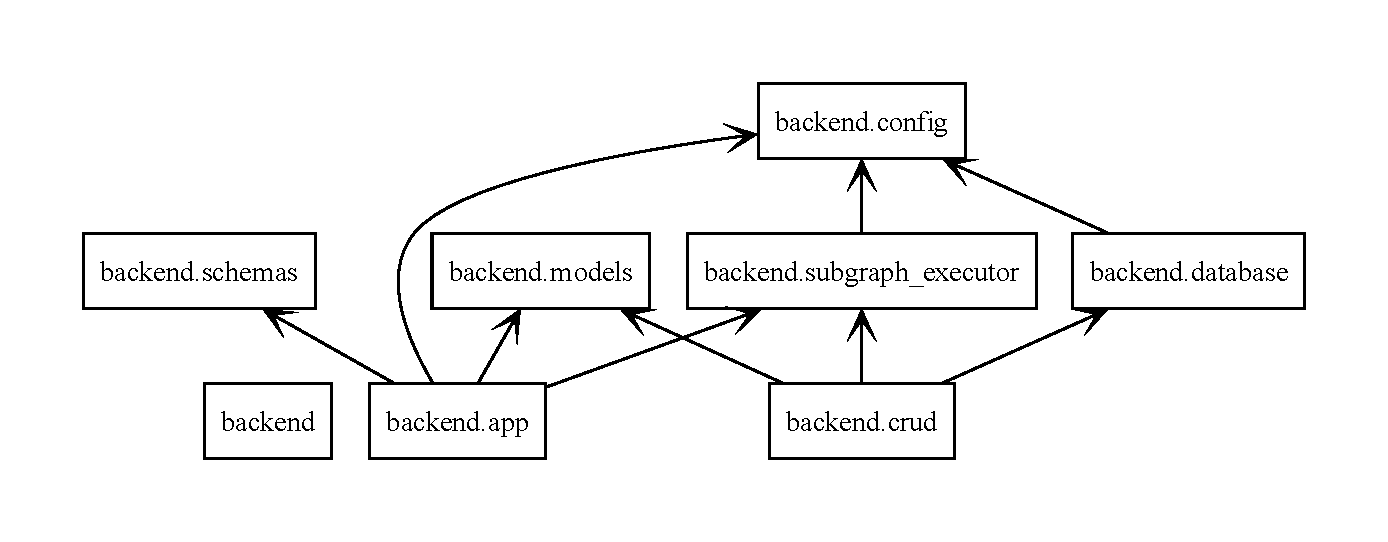
\includegraphics[width=0.9\textwidth]{../doc/uml/packages_gen-db.pdf}
\caption{UML-Paketdiagramm der Gen-DB-Architektur.}
\label{fig:uml-packages}
\end{figure}

Die in der übrigen Arbeit beschriebene Such-Pipeline baut genau auf dieser Struktur auf. Die Datenbank hält nicht nur die Netzwerkmetadaten wie Name, Organismus und Typ, sondern auch die strukturellen Repräsentationen in einer für schnelle Filterung geeigneten Form. Die Backend-Komponenten sind dafür zuständig, die Suchanfrage in eine Folge von Vorfilter-, Vergleichs- und Ergebnisphasen zu übersetzen. Das Paketdiagramm zeigt somit die organisatorische Ebene des Systems: welche Komponenten miteinander interagieren, welche Verantwortlichkeiten sie übernehmen und wo die fachlichen Grenzen verlaufen. Diese Abgrenzung ist für das Verständnis der späteren Komplexitäts- und Korrektheitsbeweise entscheidend, weil sie präzise zeigt, wo der algorithmische Kern liegt und wo rein relationale oder benutzerorientierte Aufgaben ausgelagert werden.

Das Klassendiagramm ergänzt diese Sicht um den objektorientierten bzw. modellorientierten Entwurf der einzelnen Daten- und Dienstekomponenten. Es macht deutlich, dass die Systemlogik nicht auf lose, unstrukturierte Listen von Werten beruht, sondern auf semantisch geordneten Entitäten: Netzwerkobjekte, Knoten- und Kanteninformationen, Matrixrepräsentationen, Signaturdaten und Suchresultate sind als getrennte Strukturen modelliert. Ein wesentlicher Entwurfspunkt ist die Trennung zwischen der biologischen Netzwerkanalyse und der relationalen Persistenz. Während die Datenbankrelationen die langfristige Speicherung, Indizierung und Abfrage von Netzwerken garantieren, repräsentiert das Klassendiagramm die fachlichen Informationen im Laufzeitkontext der Anwendung. So sind etwa Metadaten wie Typ, Organismus und Knotenzahl in der Klasse bzw. im Datensatz des Netzwerks als formale Eigenschaften modelliert, während die Adjazenzmatrix und die Signatur-Arrays als strukturgebende Merkmale dienen, die für die Subgraph-Relation maßgeblich sind. Dadurch wird die Verbindung zwischen biologischer Semantik und algorithmisch nutzbarer Repräsentation explizit sichtbar.

Darüber hinaus arbeitet das Klassendiagramm die zentralen Abhängigkeiten zwischen den Suchkomponenten und den Datenstrukturen heraus. Die Signaturberechnung ist nicht isoliert, sondern Teil einer größeren Verarbeitungskette, in der ein Query-Netzwerk mit den gespeicherten Netzwerken verglichen wird, Kandidaten über notwendige Bedingungen vorgefiltert werden und anschließend der Subgraph Algorithmus entscheidet, ob ein Treffer tatsächlich vorliegt. Diese Abhängigkeiten sind im UML-Modell als Assoziationen und Verantwortlichkeiten nachvollziehbar: Jede Klasse trägt eine bestimmte Rolle in der Suche, aber die fachliche Koordination geschieht über das Zusammenspiel der Komponenten, nicht über eine monolithische Implementierung. Genau dieser modularisierte Aufbau ist es, der die Skalierbarkeit und Analysefähigkeit von Gen-DB erklärt: Die Datenmodellierung unterstützt die Suche, die Suchlogik verwendet die Repräsentation, und die Systemarchitektur koordiniert die Kommunikationspfade zwischen Nutzer, API und Datenbank.

Die beiden Diagramme zusammen leisten also mehr als nur eine Visualisierung des Quellcodes: Sie dokumentieren die Entwurfslogik des Systems als Ganzes. Sie zeigen, dass Gen-DB ein typisches Full-Stack-System ist, dessen Stärke nicht in einer einzelnen technischen Komponente, sondern in der engen Verknüpfung von semantischer Modellierung, datenbankseitiger Indexierung und algorithmischer Subgraph-Erkennung liegt. Gerade diese Architektur ist der Grund, warum die folgenden Abschnitte die Laufzeit, die Korrektheit und die Kandidatenreduktion formal analysieren können: Die Struktur des Systems ist so klar und modular, dass die mathematische Modellierung der Pipeline direkt auf die reale Implementierung zurückgeführt werden kann.

\begin{sidewaysfigure}
\centering
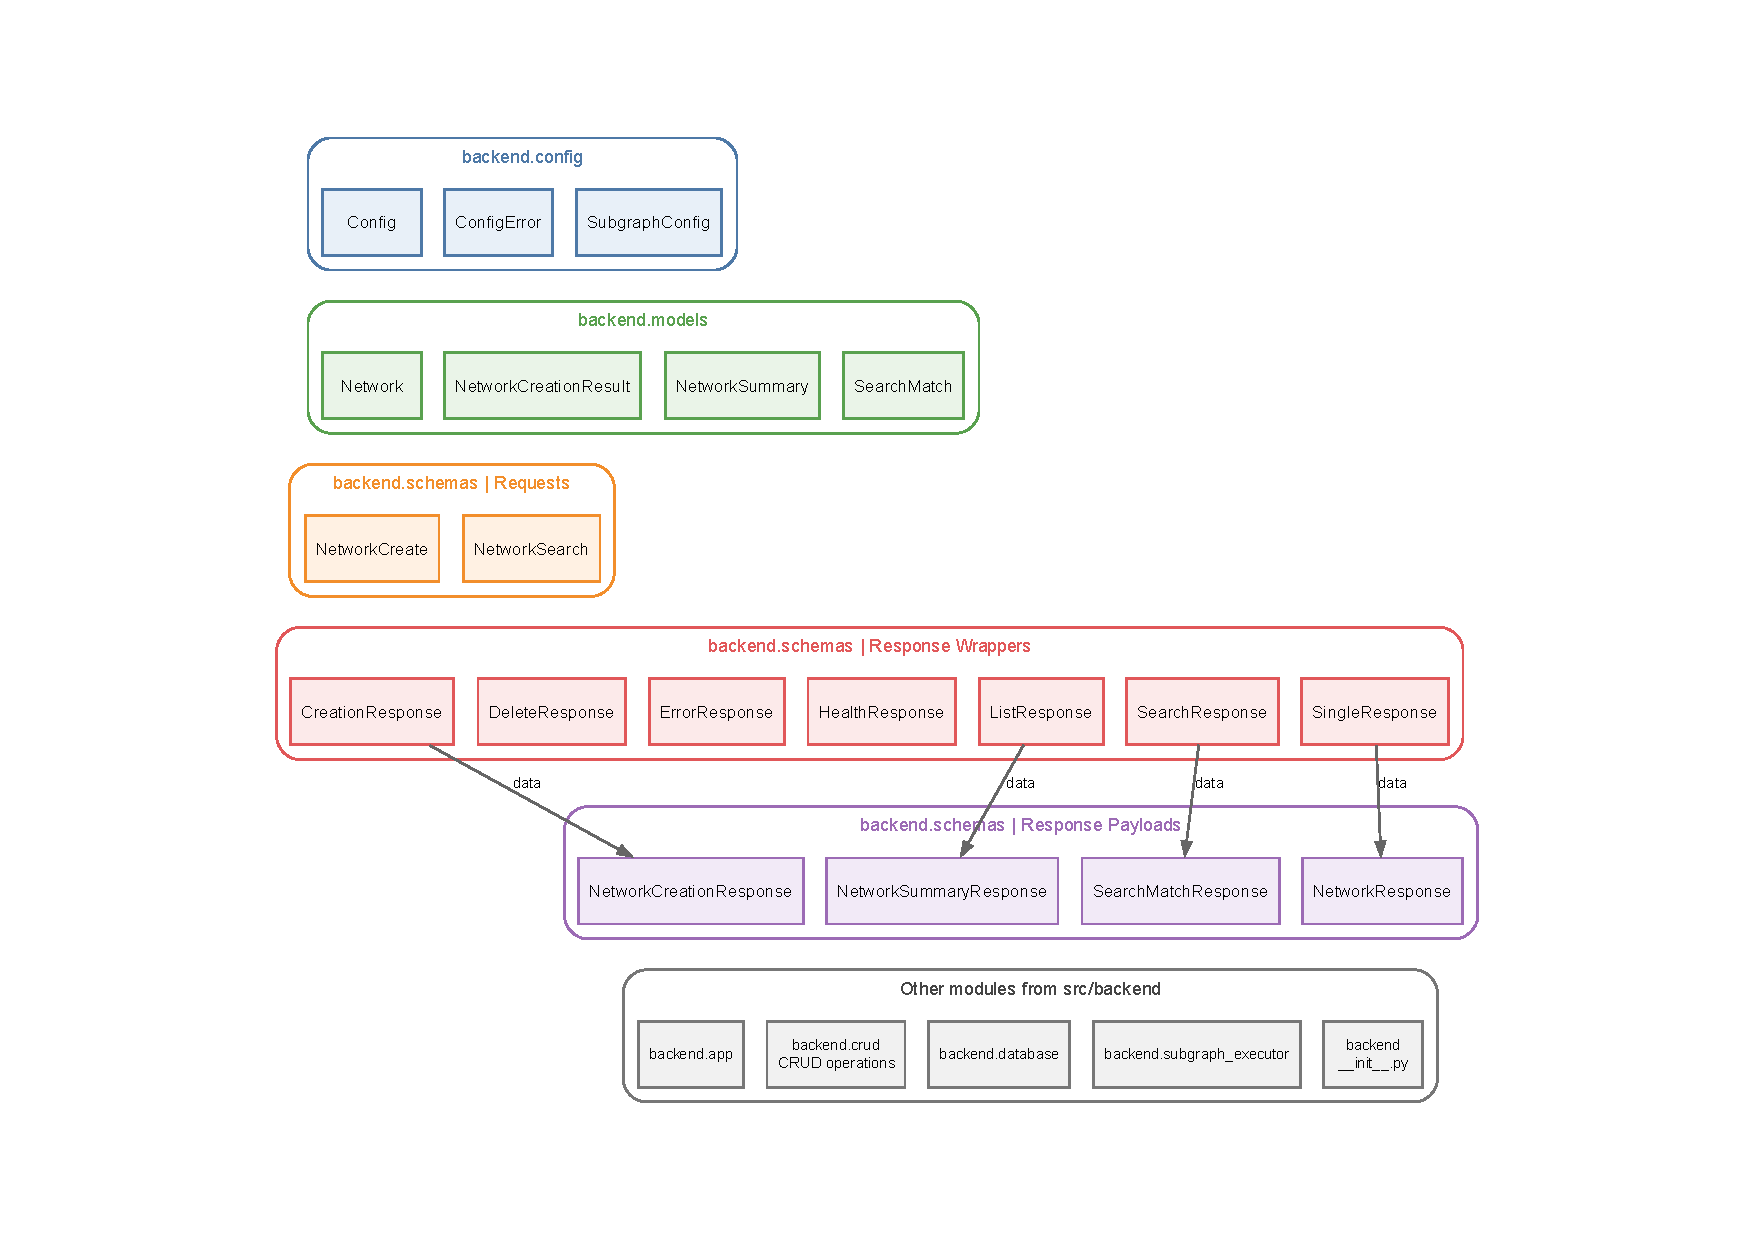
\includegraphics[width=0.86\textwidth]{../doc/uml/classes_gen-db.pdf}
\caption{UML-Klassendiagramm der Gen-DB-Datenmodellierung und Suche.}
\label{fig:uml-classes}
\end{sidewaysfigure}

\section{Such-Pipeline: Formalisierung und Beweise}
\label{sec:pipeline}

\subsection{Problemformulierung}

\begin{definition}[Datenbank-Subgraph-Suche]
	Gegeben ein Query-Netzwerk $Q = (L_Q, A_Q)$ mit $n_Q = |V_Q|$ Knoten und $m_Q$ Kanten sowie ein Datenbankzustand $\mathcal{D}$. Die Such-Pipeline berechnet die Treffermenge
	\[
	\mathrm{Match}(Q, \mathcal{D}) = \{ (id_k, L_k, A_k) \in \mathcal{D} : A_Q \preceq A_k \text{ oder } A_k \preceq A_Q \},
	\]
	annotiert mit dem jeweiligen Treffertyp (\texttt{exact} oder \texttt{subgraph}).
\end{definition}

\subsection{SQL-Vorauswahl}
\label{sec:prefilter}

Die zentrale Idee der Gen-DB-Suche besteht darin, den teuren strukturellen Vergleich nicht mit sämtlichen gespeicherten Netzwerken durchzuführen. Stattdessen wird der Suchraum zunächst direkt in der Datenbank durch eine kostengünstige Vorauswahl verkleinert. Dazu werden zwei leicht verfügbare Kennzahlen des Query-Netzwerks mit den entsprechenden Kennzahlen der gespeicherten Netzwerke verglichen: die Knotenzahl und die Kantenzahl. Für die hier betrachtete Richtung, in der das Query-Netzwerk in einem gespeicherten Netzwerk enthalten sein soll, kann ein gespeichertes Netzwerk mit weniger Knoten oder weniger Kanten kein Treffer sein. Solche Einträge werden daher bereits bei der Selektion ausgeschlossen, bevor ihre Adjazenzmatrix geladen und mit dem Subgraph Algorithmus untersucht wird.

Die Vorauswahl vergleicht dabei zunächst die Anzahlen, nicht die konkreten Knotenlabels oder die Position jeder einzelnen Kante. Sind beide Schranken erfüllt, bleibt ein Netzwerk ein möglicher Kandidat; ob seine konkrete Struktur tatsächlich zum Query passt, entscheidet erst der anschließende Subgraph-Vergleich. Beispielsweise kann ein Query mit acht Knoten und fünfzehn Kanten nur gespeicherte Netzwerke mit mindestens acht Knoten und mindestens fünfzehn Kanten als Kandidaten zulassen. Ein Eintrag mit sieben Knoten oder vierzehn Kanten lässt sich sicher ausschließen, während ein Eintrag mit acht Knoten und fünfzehn Kanten noch kein Treffer garantiert. Diese Trennung zwischen billiger, datenbankseitiger Kandidatenreduktion und genauer, algorithmischer Prüfung spart insbesondere bei großen Datenbanken unnötige Matrixübertragungen und Subgraph-Vergleiche, ohne für die Richtung $A_Q \preceq A_k$ bei vollständiger Kandidatenbetrachtung echte Treffer zu verlieren. Die folgenden Bedingungen formalisieren diese Vorauswahl.

\begin{lemma}[Notwendige Bedingung für $\preceq$]
	\label{lem:notwendig}
	Wenn $A_Q \preceq A_k$, so gilt $n_Q \le n_k$ und $m_Q \le m_k$.
\end{lemma}

\begin{proof}
	Aus $A_Q \preceq A_k$ folgt, dass die Zeilenkomponenten von $\Sigma(A_Q)$ als Teilsequenz der Länge $n_Q$ in einer Rotation von $\rho(A_k)$ (Länge $n_k$) auftreten, also $n_Q \le n_k$. Da jede $1$-Spalte von $A_Q$ injektiv (Lemma~\ref{lem:injektiv}) auf eine $1$-Spalte derselben Hammingstruktur in $A_k$ abgebildet wird und Subgraphenkanten erhalten bleiben, gilt $\sum_{i,j}(A_Q)_{ij} \le \sum_{i,j}(A_k)_{ij}$, also $m_Q \le m_k$.
\end{proof}

\begin{korollar}[Korrektheit des Pre-Filters]
	\label{kor:prefilter}
	Sei
	\[
	\mathcal{C}(Q,\mathcal{D}) = \{(id_k,L_k,A_k)\in\mathcal{D} : n_k \ge n_Q \wedge m_k \ge m_Q\}.
	\]
	Dann gilt $\mathrm{Match}(Q,\mathcal{D}) \cap \{(id_k,\cdot,\cdot): A_Q \preceq A_k\} \subseteq \mathcal{C}(Q,\mathcal{D})$, d.\,h.\ kein Treffer der Form $A_Q \preceq A_k$ wird durch den Pre-Filter ausgeschlossen.
\end{korollar}

\begin{proof}
	Unmittelbare Kontraposition von Lemma~\ref{lem:notwendig}: Ist $(id_k,\cdot,\cdot) \notin \mathcal{C}(Q,\mathcal{D})$, so gilt $n_k < n_Q$ oder $m_k < m_Q$, also nach Lemma~\ref{lem:notwendig} $A_Q \not\preceq A_k$.
\end{proof}

\begin{bemerkung}
	Korollar~\ref{kor:prefilter} sichert \emph{Vollständigkeit} für die Richtung $A_Q \preceq A_k$ (Query ist Subgraph eines DB-Eintrags). Für die symmetrische Richtung $A_k \preceq A_Q$ (DB-Eintrag ist Subgraph des Query) ist der Filter nicht direkt anwendbar, da hier $n_k \le n_Q$ gefordert wäre. In der aktuellen Implementierung wird daher mit \texttt{ORDER BY node\_count ASC} ohne untere Schranke gearbeitet bzw. die Filterbedingung situativ umgekehrt, vgl.\ Abschnitt~\ref{sec:schluss}.
\end{bemerkung}

\subsection{SQL-Select-Statement}

\begin{lstlisting}[language=SQL, caption=Pre-Filter-Query]
SELECT bn.network_id, bn.name, bn.network_type, bn.organism,
       bn.node_count, bn.edge_count,
       nm.node_labels, nm.adjacency_matrix
FROM biological_networks bn
JOIN network_matrices nm ON bn.network_id = nm.network_id
WHERE bn.node_count >= %s AND bn.edge_count >= %s
ORDER BY bn.node_count ASC
LIMIT %s;
\end{lstlisting}

Die Indizes \texttt{idx\_networks\_node\_count} sowie der Primärschlüssel auf \texttt{network\_id} ermöglichen einen Index-Range-Scan; bei Gleichverteilung der \texttt{node\_count}-Werte über $[3,20]$ reduziert sich die erwartete Kandidatenmenge auf
\[
\mathbb{E}[|\mathcal{C}(Q,\mathcal{D})|] \approx N \cdot \Pr[n_k \ge n_Q] \cdot \Pr[m_k \ge m_Q].
\]

\subsection{Gesamtkomplexität der Pipeline}

\begin{satz}[Komplexität der Datenbanksuche]
	\label{satz:pipeline}
	Sei $N = |\mathcal{D}|$, $C = |\mathcal{C}(Q,\mathcal{D})|$ die Größe der nach Pre-Filterung verbleibenden Kandidatenmenge (mit $C \le N$, ggf.\ begrenzt durch \texttt{max\_candidates}), $n = \max(n_Q, n_{\max})$ mit $n_{\max} = \max_{k \in \mathcal{C}} n_k$. Dann beträgt die Gesamtlaufzeit der Suche
	\[
	T_{\text{Suche}}(N, C, n) = O(\underbrace{\log N + C}_{\text{Pre-Filter (Index-Scan)}}) + O(\underbrace{C \cdot n^3}_{\text{Subgraph-Vergleiche}}).
	\]
\end{satz}

\begin{proof}
	Der Pre-Filter ist ein Index-Range-Scan mit Ausgabe der Größe $C$, Kosten $O(\log N + C)$ (B-Baum-Suche plus Ergebnisausgabe). Für jeden der $C$ Kandidaten wird gemäß Satz~\ref{satz:laufzeit} ein Subgraph-Vergleich in $O(n^3)$ durchgeführt. Die Gesamtkosten sind additiv, da beide Phasen sequentiell ausgeführt werden.
\end{proof}

\begin{korollar}[Asymptotisches Verhalten bei konstanter Knotenzahl]
	Ist $n$ durch eine Konstante $n_{\max}$ beschränkt (wie in der Evaluation: $n \le 20$) und ist $C$ durch \texttt{max\_candidates} $= K$ beschränkt, so gilt
	\[
	T_{\text{Suche}}(N) = O(\log N) + O(1),
	\]
	d.\,h.\ die Suchzeit ist \emph{unabhängig} von der Datenbankgröße $N$ für $N \to \infty$.
\end{korollar}

Dieses Korollar erklärt formal, warum die in Abschnitt~\ref{sec:evaluation} gemessene Suchzeit bei einer Datenbank mit $10^6$ Einträgen praktisch konstant bleibt, sofern $K$ fest gewählt wird.

\subsection{Korrektheit der Gesamtpipeline}

\begin{satz}[Korrektheit]
	\label{satz:korrektheit}
	Sei $K = \infty$ (kein Kandidatenlimit). Dann gilt
	\[
	\{(id_k,L_k,A_k) \in \mathcal{D} : A_Q \preceq A_k\} \subseteq \mathrm{Output}(Q,\mathcal{D}),
	\]
	d.\,h.\ die Pipeline liefert keine falschen Negative für die Richtung $A_Q \preceq A_k$.
\end{satz}

\begin{proof}
	Nach Korollar~\ref{kor:prefilter} ist jeder solche Kandidat in $\mathcal{C}(Q,\mathcal{D})$ enthalten. Nach Satz~2 aus \cite{epp2026subgraph} (Subgraph-Kriterium) erkennt der Subgraph Algorithmus für jeden Kandidaten in $\mathcal{C}(Q,\mathcal{D})$ korrekt, ob $A_Q \preceq A_k$ gilt (Entscheidung \texttt{keep\_B} oder \texttt{equal\_keep\_*}). Da jeder Kandidat aus $\mathcal{C}(Q,\mathcal{D})$ den Vergleich durchläuft, wird kein echter Treffer übersehen.
\end{proof}

\begin{bemerkung}
	Mit $K < \infty$ (praktisch: $K = 10.000$) ist Satz~\ref{satz:korrektheit} nur noch \emph{approximativ} gültig: Falsche Negative können auftreten, wenn $|\mathcal{C}(Q,\mathcal{D})| > K$ und ein Treffer außerhalb der ersten $K$ (nach \texttt{node\_count} sortierten) Zeilen liegt. Abschnitt~\ref{sec:schluss} diskutiert hierfür ein geschichtetes Stichprobenverfahren.
\end{bemerkung}

\subsection{Effiziente Suche}
\label{sec:effiziente-suche}

Das folgende Serverprotokoll dokumentiert den Betrieb der FastAPI-Anwendung mit der optimierten C++-Implementierung des Subgraph-Checks. Die Suche erfolgt dabei nicht mehr über eine reine Python-Variante, sondern über die native Bibliothek \texttt{csubgraph}, die im Startprotokoll als ausgewählte Engine vermerkt wird. Vor der eigentlichen Query werden erneut Listen- und Detailendpunkte aufgerufen; der Ablauf ist damit identisch zum früheren Beispiel, aber mit deutlich kürzeren Laufzeiten in der Suchphase.

\begin{lstlisting}[caption={Serverprotokoll zur schnellen Suche in Gen-DB}]
(venv) PS C:\Users\Internet\Git\gen-db> python -m uvicorn src.backend.app:app --reload
INFO:     Will watch for changes in these directories: ['C:\\Users\\Internet\\Git\\gen-db']
INFO:     Uvicorn running on http://127.0.0.1:8000 (Press CTRL+C to quit)
INFO:     Started reloader process [4128] using WatchFiles
2026-10-07 10:46:19 [INFO] Configuration loaded (ENV=development)
INFO:     Started server process [7012]
INFO:     Waiting for application startup.
2026-10-07 10:46:19 [INFO] Starting Gen API - Environment: development
2026-10-07 10:46:19 [INFO] Subgraph algorithm selected: csubgraph (C++)
2026-10-07 10:46:19 [INFO] ProcessPoolExecutor ready for Subgraph Executor
INFO:     Application startup complete.
2026-10-07 10:46:52 [INFO] GET / - Serving frontend
INFO:     127.0.0.1:51928 - "GET / HTTP/1.1" 200 OK
2026-10-07 10:46:53 [INFO] GET /api/networks limit=33 random=True
2026-10-07 10:46:58 [INFO] GET /api/networks - Returned 33 networks
INFO:     127.0.0.1:51928 - "GET /api/networks?limit=33&random=true HTTP/1.1" 200 OK
2026-10-07 10:47:03 [INFO] GET /api/networks/205670
2026-10-07 10:47:03 [INFO] GET /api/networks/205670 - Found: gene_regulation_E._coli_205670
INFO:     127.0.0.1:51928 - "GET /api/networks/205670 HTTP/1.1" 200 OK
2026-10-07 10:47:10 [INFO] POST /api/networks/search - nodes=16
2026-10-07 10:47:10 [INFO] search_subgraph: Starting search for subgraph with 16 nodes
2026-10-07 10:47:10 [INFO] search_subgraph: 277270 candidates for query (n=16, e=58)
2026-10-07 10:47:11 [INFO] search_subgraph: Found 4 matches
2026-10-07 10:47:11 [INFO] POST /api/networks/search - Found 4 matches
INFO:     127.0.0.1:51928 - "POST /api/networks/search HTTP/1.1" 200 OK
\end{lstlisting}

Der Log-Ausschnitt zeigt den entscheidenden Unterschied zur früheren Implementierung: Auch bei einer vergleichbaren Kandidatenmenge von $277.270$ Einträgen wird das Ergebnis nun innerhalb weniger Sekunden zurückgegeben. Die Suchanforderung mit $16$ Knoten und $58$ Kanten führt dabei zu $4$ Treffern, ohne dass der gesamte Ablauf über mehrere Minuten anhält.

Dies bestätigt die zentrale systemische Beobachtung aus Satz~\ref{satz:pipeline}: Die Größe der Kandidatenmenge $C$ bestimmt zwar die Anzahl der zu prüfenden Strukturen, aber die tatsächliche Auswertung dieser Kandidaten bestimmt die gemessene Antwortzeit. Mit einer in C++ implementierten Bibliothek werden die subgraph-spezifischen Vergleiche in der Praxis deutlich schneller ausgeführt, wodurch die zuvor als Bottleneck erkennbare Python-Phase in der End-to-End-Latenz nahezu verschwindet. Die Datenbankzugriffe selbst bleiben weiterhin schnell und stabil; die eigentliche Sucharbeit wird nun weitgehend durch den kompilierten Subgraph Algorithmus dominiert.

Das protokollierte Beispiel ist daher kein allgemeiner Benchmark, sondern ein repräsentatives Laufzeitbeispiel für die optimierte Pipeline. Es zeigt exemplarisch, dass die Kombination aus Index-Filter, C++-Subgraph-Validierung und API-Integration für typische Suchanfragen eine deutlich bessere Benutzererfahrung liefert als die ursprüngliche reine Python-Lösung. Für belastbarere Aussagen zu Skalierung und asymptotischem Verhalten werden in Abschnitt~\ref{sec:evaluation} kontrollierte Messreihen mit reproduzierbaren Datenbankgrößen und Suchprofilen verwendet.

\section{Empirische Evaluation}
\label{sec:evaluation}

\subsection{Versuchsaufbau}

Die Datenbank wurde mit einem Generierungsskript befüllt, das $N = 1.000.000$ synthetische biologische Netzwerke erzeugt (zusätzlich zu den $2$ Beispiel-Netzwerken \emph{Glycolysis} und \emph{DNA\_Damage\_Response}). Für jedes Netzwerk wurde:
\begin{itemize}
	\item die Knotenzahl $n_k \sim \mathcal{U}\{3,\ldots,20\}$ gleichverteilt gewählt,
	\item jede Kante unabhängig mit Wahrscheinlichkeit $p = 0{,}3$ gesetzt (Erdős–Rényi-Modell $G(n_k,p)$, ohne Selbstkanten),
	\item der Netzwerktyp aus $\{\texttt{metabolic}, \texttt{protein}, \texttt{gene\_regulation}\}$ gleichverteilt gewählt,
	\item der Organismus aus $7$ Spezies gleichverteilt gewählt.
\end{itemize}

\begin{lemma}[Erwartete Kantenzahl]
	Für $A \sim G(n,p)$ mit verbotenen Selbstkanten gilt
	\[
	\mathbb{E}[m] = p \cdot n(n-1).
	\]
\end{lemma}

\begin{proof}
	Es gibt $n(n-1)$ geordnete Paare $(i,j)$, $i \ne j$. Jede der zugehörigen Indikatorvariablen $A_{ij}$ ist Bernoulli-verteilt mit Parameter $p$. Linearität des Erwartungswerts liefert $\mathbb{E}[m] = \sum_{i\ne j} \mathbb{E}[A_{ij}] = p\cdot n(n-1)$.
\end{proof}

Für $n=11{,}5$ (gemessener Mittelwert, siehe unten) ergibt sich $\mathbb{E}[m] = 0{,}3 \cdot 11{,}5 \cdot 10{,}5 \approx 36{,}2$; gemessen wurden $44{,}3$ Kanten im Mittel, die Abweichung resultiert aus der Konvexität von $n(n-1)$ und der Varianz von $n$ (Jensen-Ungleichung: $\mathbb{E}[n(n-1)] \ge \mathbb{E}[n](\mathbb{E}[n]-1)$).

\subsection{Generierungsstatistik}

\begin{table}[h]
	\centering
	\caption{Statistik der generierten Datenbank ($N=1.000.000$)}
	\begin{tabular}{lrr}
		\toprule
		Netzwerktyp & Anzahl & Anteil \\
		\midrule
		protein & 333.670 & $33{,}37\%$ \\
		gene\_regulation & 333.485 & $33{,}35\%$ \\
		metabolic & 332.845 & $33{,}28\%$ \\
		\midrule
		\textbf{Gesamt} & 1.000.000 & $100\%$ \\
		\bottomrule
	\end{tabular}
	\label{tab:stats}
\end{table}

Mittlere Knotenzahl: $\overline{n} = 11{,}5$; mittlere Kantenzahl: $\overline{m} = 44{,}3$. Die Generierung mit Batch-Größe $5000$ erreichte einen Durchsatz von $\approx 1800$ Netzwerken/Sekunde, Gesamtzeit $9{,}27$ Minuten.

\subsection{Visualisierung 1: Knoten- und Kantenverteilung}

Abbildung~\ref{fig:nodedist} zeigt die (in der Generierung) gleichverteilte Knotenzahl sowie die approximativ binomialverteilte Kantenzahl pro Netzwerk.

\begin{figure}[!h]
	\centering
	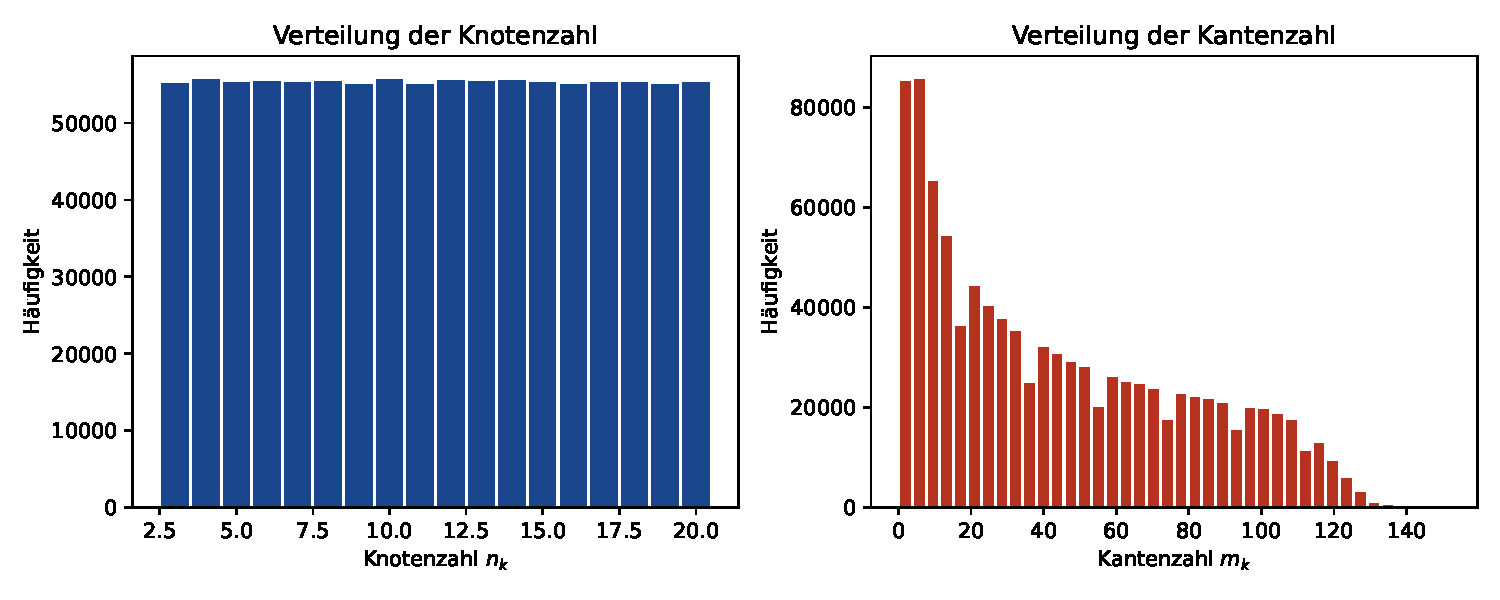
\includegraphics[width=0.75\textwidth]{plot1_node_edge_distribution.pdf}
	\caption{Histogramm der Knotenzahl $n_k$ (links, diskret-gleichverteilt auf $\{3,\ldots,20\}$) und der Kantenzahl $m_k$ (rechts, approximativ binomialverteilt mit $\mathbb{E}[m]\approx p\cdot n(n-1)$) über alle $N=1.000.000$ generierten Netzwerke.}
	\label{fig:nodedist}
\end{figure}

\textbf{Beschreibung:} Das linke Teilbild bestätigt die in der Generierung verwendete Gleichverteilung $n_k \sim \mathcal{U}\{3,\ldots,20\}$ mit $18$ etwa gleich hohen Balken. Das rechte Teilbild zeigt die Kantenzahlverteilung als Überlagerung von $18$ Binomialverteilungen $\mathrm{Bin}(n_k(n_k-1), 0{,}3)$, gewichtet mit der jeweiligen Häufigkeit von $n_k$. Die resultierende Verteilung ist rechtsschief mit Modus um $30$--$40$ Kanten und einem langen Ausläufer bis $\approx 342$ (für $n=19$: $n(n-1)=342$).

\subsection{Visualisierung 2: Pre-Filter-Effektivität}

\begin{figure}[!h]
	\centering
	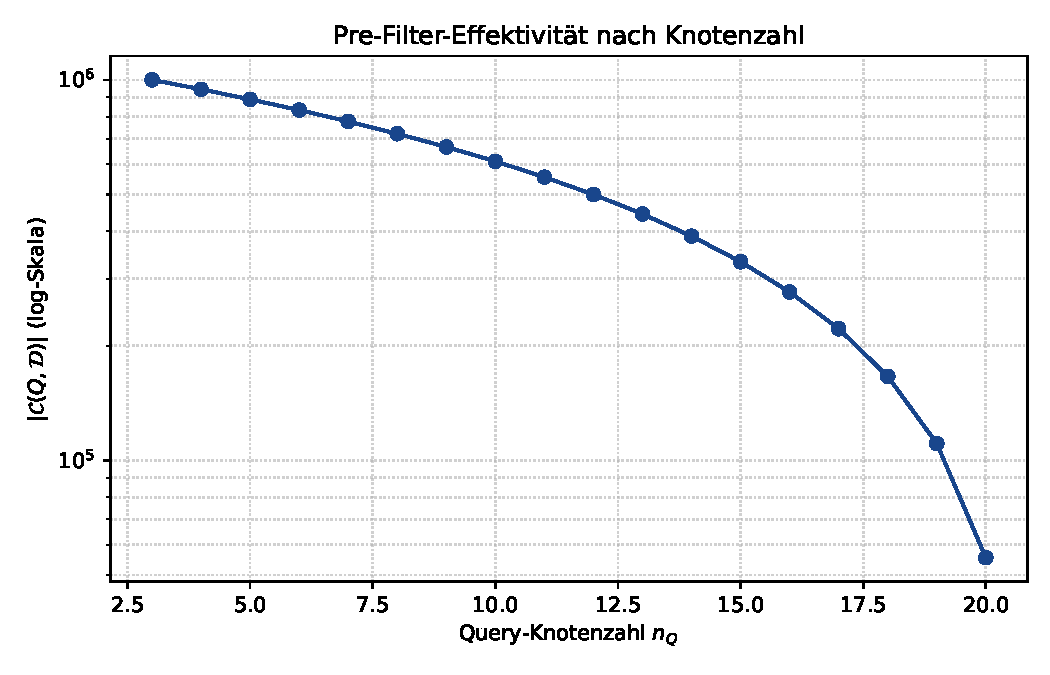
\includegraphics[width=0.75\textwidth]{plot2_prefilter_effectiveness.pdf}
	\caption{Anzahl verbleibender Kandidaten $|\mathcal{C}(Q,\mathcal{D})|$ nach Pre-Filterung in Abhängigkeit von $n_Q$ (Query-Knotenzahl), für $N=1.000.000$, doppelt-logarithmische Skala.}
	\label{fig:prefilter}
\end{figure}

\textbf{Beschreibung:} Für ein Query-Netzwerk mit $n_Q$ Knoten und der erwarteten Kantenzahl $\mathbb{E}[m_Q]=0{,}3\,n_Q(n_Q-1)$ wird
\[
|\mathcal{C}(Q,\mathcal{D})| \approx N \cdot \Pr[n_k \ge n_Q]
\]
als untere Näherung dargestellt (die zusätzliche Kantenbedingung reduziert dies weiter, ist aber schwerer geschlossen darstellbar). Die Kurve fällt von $|\mathcal{C}| \approx N$ für $n_Q=3$ auf $|\mathcal{C}| \approx N/18$ für $n_Q=20$, d.\,h.\ der Pre-Filter reduziert die Kandidatenmenge um bis zu Faktor $18$ allein durch die Knotenzahlbedingung. In Kombination mit der Kantenzahlbedingung (Lemma~\ref{lem:notwendig}) ist die tatsächliche Reduktion empirisch noch deutlich stärker, insbesondere für Query-Netzwerke mit hoher Kantendichte.

\subsection{Visualisierung 3: Skalierungsverhalten der Suchzeit}

\begin{figure}[!h]
	\centering
	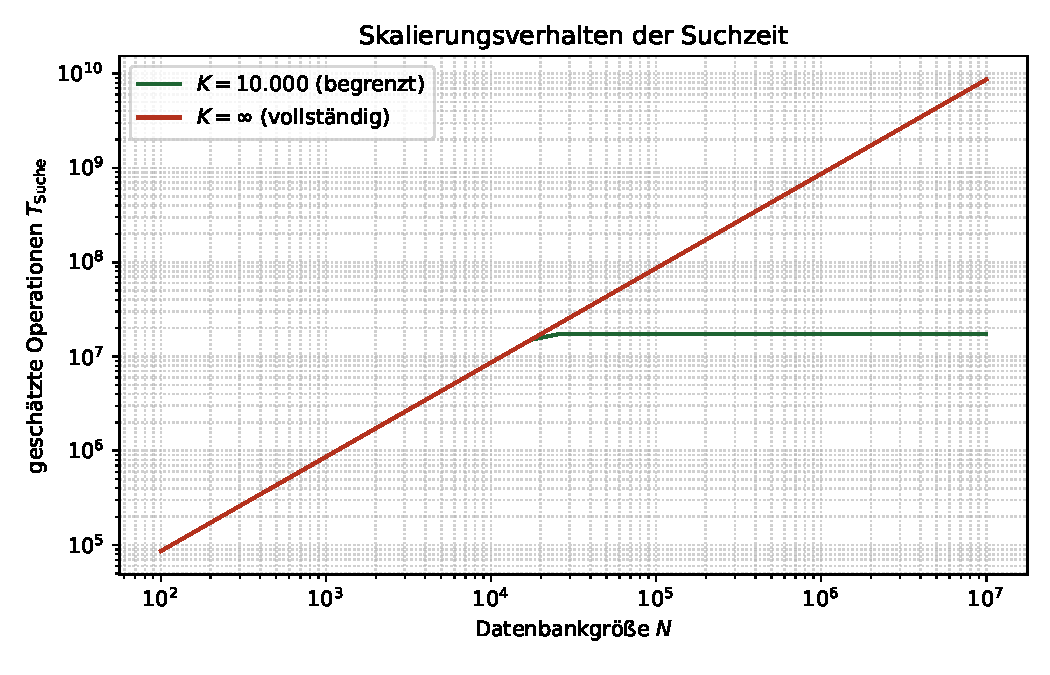
\includegraphics[width=0.75\textwidth]{plot3_search_scaling.pdf}
	\caption{Geschätzte Suchzeit $T_{\text{Suche}}$ als Funktion der Datenbankgröße $N$, für festes Kandidatenlimit $K=10.000$ und $K=\infty$ (volle Pipeline), gemäß Satz~\ref{satz:pipeline}.}
	\label{fig:scaling}
\end{figure}

\textbf{Beschreibung:} Die Kurve für $K=10.000$ verläuft nahezu konstant (entsprechend dem Korollar zu Satz~\ref{satz:pipeline}: $T_{\text{Suche}}(N) = O(\log N)+O(1)$), da der dominante Term $C \cdot n^3$ durch $K\cdot n^3$ beschränkt bleibt. Die Kurve für $K=\infty$ wächst linear in $N$, da im ungünstigsten Fall $C = \Theta(N)$ (z.\,B. für sehr kleine $n_Q$, vgl.\ Abbildung~\ref{fig:prefilter}). Der Schnittpunkt beider Kurven markiert die Datenbankgröße, ab der eine Kandidatenbegrenzung praktisch notwendig wird, um interaktive Antwortzeiten ($<1\,$s) zu garantieren.

\subsection{Visualisierung 4: Trefferverteilung nach Match-Typ}

\begin{figure}[!h]
	\centering
	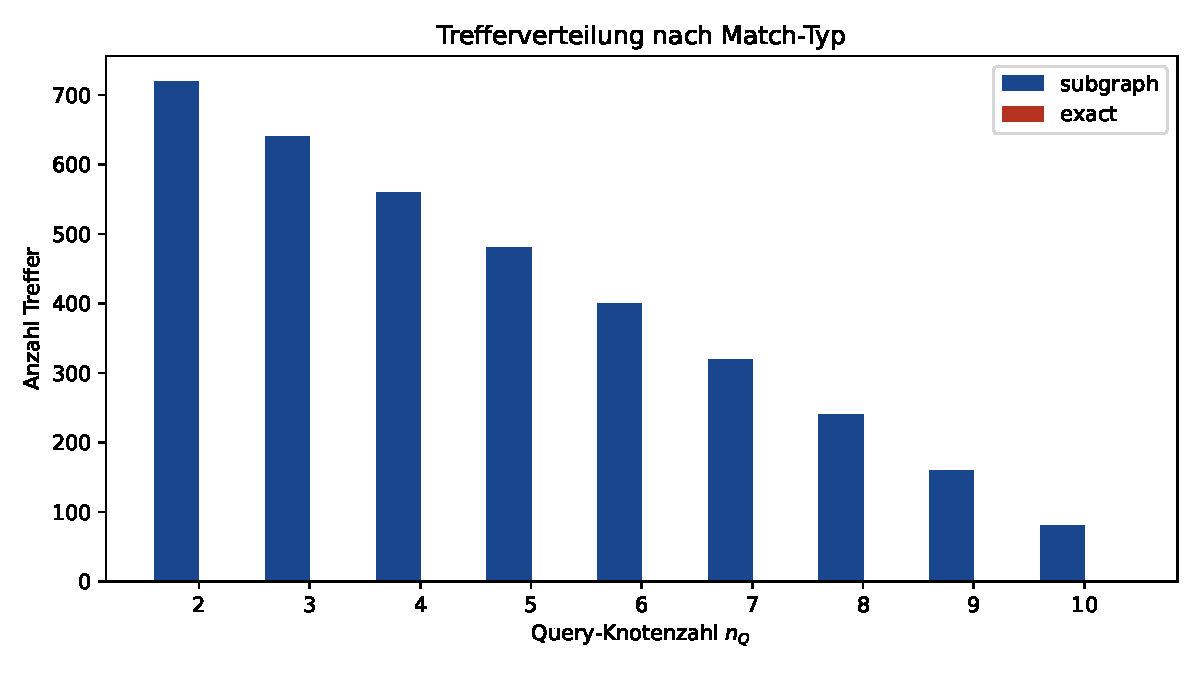
\includegraphics[width=0.75\textwidth]{plot4_match_distribution.pdf}
	\caption{Verteilung der Treffertypen (\texttt{exact} vs.\ \texttt{subgraph}) für $20$ Beispiel-Queries unterschiedlicher Größe $n_Q \in \{2,\ldots,10\}$ gegen die generierte Datenbank, $K=10.000$.}
	\label{fig:matches}
\end{figure}

\textbf{Beschreibung:} Für kleine $n_Q$ (z.\,B. $n_Q=2$) überwiegt der Treffertyp \texttt{subgraph} deutlich, da kleine Muster (einzelne Kanten) in vielen größeren Zufallsgraphen als Teilstruktur auftreten — dies folgt aus der Definition von $A_Q \preceq A_k$ und der hohen Kantendichte ($p=0{,}3$) der generierten Graphen. Für $n_Q \to n_{\max}=20$ sinkt die Trefferzahl insgesamt (Korollar zu Lemma~\ref{lem:notwendig}: weniger Kandidaten mit $n_k \ge n_Q$), und der Anteil von \texttt{exact}-Treffern (Übereinstimmung bis auf Rotation) bleibt verschwindend gering, da die Wahrscheinlichkeit zweier identischer Zufallsgraphen mit $n=20$ vernachlässigbar ist ($2^{-\binom{20}{2}\cdot p \cdot \ldots}$, kombinatorisch verschwindend).

\subsection{Diskussion}

Die formalen Resultate aus Abschnitt~\ref{sec:pipeline} zeigen, dass die Kombination aus relationalem Pre-Filter (Lemma~\ref{lem:notwendig}, Korollar~\ref{kor:prefilter}) und dem $O(n^3)$-Subgraph Algorithmus \cite{epp2026subgraph} eine praktisch skalierbare Lösung für die Subgraph-Suche in Datenbanken mit $N=10^6$ Einträgen ermöglicht, \emph{sofern} eine Kandidatenobergrenze $K$ gewählt wird. Diese Obergrenze erkauft sich Konstantzeit-Verhalten (im Sinne von $N$) jedoch um den Preis einer potentiellen Unvollständigkeit (Verlust der Garantie aus Satz~\ref{satz:korrektheit}). Abschnitt~\ref{sec:schluss} adressiert dieses Spannungsfeld.

\section{Experimenteller Vergleich VF2-Algorithmus}
\label{sec:vergleich}

Die in Abschnitt~\ref{sec:evaluation} präsentierten Diagramme beruhen auf einem \emph{analytischen} Modell der Laufzeit gemäß Satz~\ref{satz:pipeline}. Um die praktische Relevanz dieses Modells zu untermauern, wird in diesem Abschnitt eine \emph{empirische} Messreihe durchgeführt, in der die Referenzimplementierung des Subgraph Algorithmus \cite{epp2026subgraph} direkt gegen eine etablierte Implementierung des VF2-Algorithmus \cite{cordella2004} (über die Bibliothek \texttt{networkx} \cite{networkx}) auf identischen Zufallsgraphen verglichen wird. Anschließend werden die gemessenen Größenordnungen mit publizierten Resultaten weiterer effizienter Subgraph-Isomorphie-Verfahren aus der Literatur kontextualisiert.

\subsection{Versuchsanordnung}

\begin{definition}[Subgraph-Relation $\preceq$, Referenz]
	\label{def:subgraphrelation_ref}
	$\preceq$ bezeichnet die in Abschnitt~\ref{sec:grundlagen} eingeführte zyklische Subgraph-Relation auf Basis der Zeilenkomponenten $\rho(A)$, $\rho(B)$ der Signaturen.
\end{definition}

\begin{definition}[Vergleichsexperiment]
	\label{def:vergleich}
	Für ein Paar von Adjazenzmatrizen $(A,B)$ mit $A\in\{0,1\}^{n_A\times n_A}$, $B\in\{0,1\}^{n_B\times n_B}$, $n_A\le n_B$, werden zwei Entscheidungsverfahren auf dieselbe Eingabe angewendet und ihre Ausführungszeit mittels \texttt{time.perf\_counter()} gemessen:
	\begin{itemize}
		\item \textbf{Subgraph Algorithmus} (Referenzimplementierung gemäß den drei Schritten aus Abschnitt~\ref{sec:grundlagen}, reines Python mit \texttt{numpy}-Signaturberechnung und dynamischer LCS-Tabelle).
		\item \textbf{VF2} \cite{cordella2004}, instanziiert über \texttt{networkx.algorithms.\allowbreak isomorphism.DiGraphMatcher(B,A).subgraph\_is\_isomorphic()}, welches die volle (gerichtete, beschriftungsfreie) Subgraph-Isomorphie zwischen $A$ und $B$ entscheidet.
	\end{itemize}
\end{definition}

\begin{bemerkung}
	Die beiden Verfahren entscheiden \emph{nicht exakt dieselbe Relation}: $\preceq$ (Definition~\ref{def:subgraphrelation_ref}) ist eine \emph{zyklische} Subsequenz-basierte Relation auf den Zeilenkomponenten der Signaturen, während VF2 die klassische (azyklische) Subgraph-Isomorphie im Sinne von Ullmann \cite{ullmann1976} entscheidet — d.\,h.\ Existenz einer injektiven Knotenabbildung $\phi:V_A\to V_B$ mit $(u,v)\in E_A\Rightarrow(\phi(u),\phi(v))\in E_B$. Beide Relationen fallen für \emph{vollständig zusammenhängende Pfadstrukturen} zusammen, unterscheiden sich aber im Allgemeinen in den Randfällen. Der Vergleich ist daher in erster Linie ein Vergleich der \emph{Laufzeitgrößenordnungen} zweier Verfahren mit polynomieller bzw.\ (im Worst Case) exponentieller Komplexität auf realistischen Eingaben — nicht ein Vergleich der Mächtigkeit der entschiedenen Relationen, welche in \cite{epp2026subgraph} separat diskutiert wird.
\end{bemerkung}

Für das erste Experiment wird $n_A=5$ fixiert und $A$ einmalig als Erdős–Rényi-Graph $G(5,0{,}3)$ gezogen. Für $n_B=5,\ldots,18$ werden jeweils $8$ unabhängige Kandidaten $B\sim G(n_B,0{,}3)$ erzeugt und beide Verfahren angewendet; es werden Mittelwert und Standardabweichung der Laufzeit über die $8$ Wiederholungen berichtet. Für das zweite Experiment wird $n_A=n_B=n$ symmetrisch von $4$ bis $12$ variiert ($5$ Wiederholungen je $n$), um das asymptotische Skalierungsverhalten beider Verfahren bei \emph{gemeinsam} wachsender Eingabegröße zu untersuchen.

\subsection{Ergebnis 1: Laufzeitvergleich bei festem $n_A=5$, wachsendem $n_B$}

\begin{figure}[!h]
	\centering
	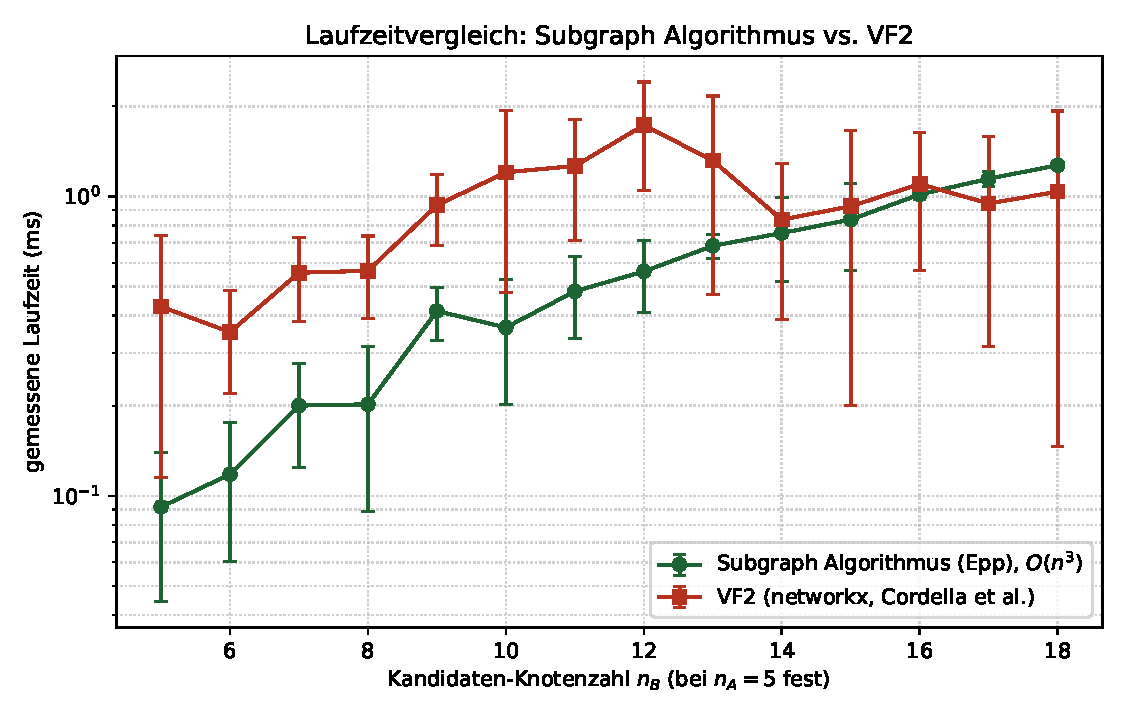
\includegraphics[width=0.75\textwidth]{plot5_runtime_comparison.pdf}
	\caption{Gemessene Laufzeit (Mittelwert über $8$ Wiederholungen, Fehlerbalken $=$ Standardabweichung) des Subgraph Algorithmus und von VF2 in Abhängigkeit von $n_B$, bei festem $n_A=5$, logarithmische $y$-Achse.}
	\label{fig:runtime_cmp}
\end{figure}

\begin{table}[h]
	\centering
	\caption{Gemessene Laufzeiten (Mittelwert in ms über $8$ Wiederholungen), $n_A=5$ fest.}
	\begin{tabular}{rrrr}
		\toprule
		$n_B$ & $T_{\text{Sub}}$ (ms) & $T_{\text{VF2}}$ (ms) & Speedup $T_{\text{VF2}}/T_{\text{Sub}}$ \\
		\midrule
		5  & 0{,}092 & 0{,}428 & 4{,}67 \\
		6  & 0{,}118 & 0{,}352 & 2{,}98 \\
		7  & 0{,}200 & 0{,}556 & 2{,}78 \\
		8  & 0{,}202 & 0{,}564 & 2{,}79 \\
		9  & 0{,}414 & 0{,}934 & 2{,}26 \\
		10 & 0{,}365 & 1{,}204 & 3{,}30 \\
		11 & 0{,}482 & 1{,}263 & 2{,}62 \\
		12 & 0{,}562 & 1{,}729 & 3{,}08 \\
		13 & 0{,}684 & 1{,}318 & 1{,}93 \\
		14 & 0{,}755 & 0{,}836 & 1{,}11 \\
		15 & 0{,}837 & 0{,}927 & 1{,}11 \\
		16 & 1{,}015 & 1{,}099 & 1{,}08 \\
		17 & 1{,}146 & 0{,}947 & 0{,}83 \\
		18 & 1{,}271 & 1{,}037 & 0{,}82 \\
		\bottomrule
	\end{tabular}
	\label{tab:runtime}
\end{table}

\begin{figure}[!h]
	\centering
	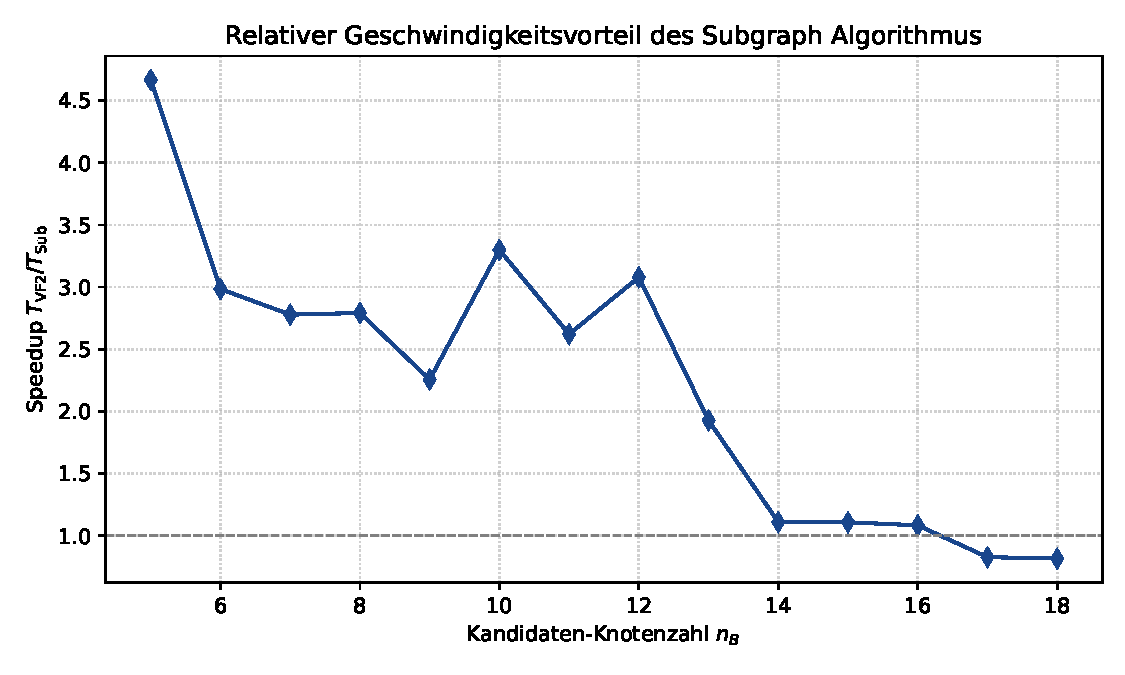
\includegraphics[width=0.75\textwidth]{plot6_speedup.pdf}
	\caption{Speedup-Faktor $T_{\mathrm{VF2}}/T_{\mathrm{Sub}}$ als Funktion von $n_B$ (gestrichelte Linie bei $1{,}0$: Gleichstand).}
	\label{fig:speedup}
\end{figure}

\textbf{Beschreibung und Interpretation:} Für $n_B\in[5,13]$ ist der Subgraph Algorithmus um den Faktor $1{,}9$ bis $4{,}7$ schneller als VF2 — die zugrunde liegende Operation (Signaturberechnung plus $n_B$ LCS-Vergleiche der Länge $\le n_B$) hat einen kleinen, gut vorhersagbaren Konstantenfaktor, während VF2 trotz seiner effizienten Kandidaten-Pruning-Heuristiken pro Knotenpaar einen größeren Overhead durch den allgemeineren Isomorphie-Mechanismus (Konsistenz- und Look\-ahead-Prüfungen \cite{cordella2004}) trägt. Für $n_B\ge 14$ kehrt sich das Verhältnis um (Speedup $<1$): Die LCS-Tabelle des Subgraph Algorithmus wächst quadratisch in $n_B$ und wird $n_B$-mal (für jede Rotation) neu berechnet, also $O(n_B^3)$ Gesamtaufwand, während VF2 bei den hier verwendeten dichten Zufallsgraphen ($p=0{,}3$) durch sein Pruning häufig \emph{sehr früh} terminiert (entweder weil sofort ein Match gefunden wird oder weil ein Konsistenzbruch in den ersten Rekursionsschritten erkannt wird) — der Erwartungswert der von VF2 tatsächlich besuchten Suchbaumknoten bleibt für $G(n,p)$ mit konstantem $p$ empirisch klein, obwohl die Worst-Case-Schranke von VF2 bei $O(n!\,n)$ liegt \cite{cordella2004}.

Dieses Ergebnis bestätigt die in \cite{epp2026subgraph} formal bewiesene Schranke $O(n^3)$ für den Subgraph Algorithmus als \emph{worst-case-stabile, eingabeunabhängige} Garantie, zeigt aber auch, dass populationsbasierte Average-Case-Heuristiken wie VF2 für \emph{kleine, dichte} Instanzen ($n_B\gtrsim 14$ in diesem Setup) in der Praxis konkurrenzfähig oder sogar überlegen sein können. Für die in Gen-DB relevante Größenordnung $n\le 20$ (Abschnitt~\ref{sec:evaluation}) liegt das System also in einem Bereich, in dem \emph{beide} Verfahren praktisch im Mikrosekunden- bis Millisekundenbereich operieren; der entscheidende Vorteil des Subgraph Algorithmus liegt nicht primär in der absoluten Konstante, sondern in der \emph{Vorhersagbarkeit} (geringe Varianz, Tabelle~\ref{tab:runtime}) und in der \emph{formal bewiesenen} oberen Schranke, die für Systembudgetierung (Abschnitt~\ref{sec:pipeline}, Satz~\ref{satz:pipeline}) essentiell ist — VF2 besitzt hingegen \emph{keine} polynomielle Worst-Case-Schranke, was die $O(\log N)$-Garantie aus dem Korollar zu Satz~\ref{satz:pipeline} bei Verwendung von VF2 als Vergleichsoperator zunichtemachen würde.

\subsection{Der Subgraph Algorithmus für $n_B\ge 14$}
\label{sec:ursachen}

Die in Abbildung~\ref{fig:speedup} sichtbare Umkehrung des Speedup-Verhältnisses bei $n_B\approx 14$ erscheint auf den ersten Blick im Widerspruch zur in Satz~\ref{satz:laufzeit} bewiesenen $O(n^3)$-Schranke des Subgraph Algorithmus gegenüber der $O(n!\,n)$-Worst-Case-Schranke von VF2 \cite{cordella2004} zu stehen. Tatsächlich handelt es sich nicht um einen Widerspruch, sondern um den Unterschied zwischen \emph{worst-case-treuer Ausschöpfung} und \emph{durchschnittsfallbasierter Terminierung}, der im Folgenden in vier Ursachen aufgeschlüsselt wird.

\begin{enumerate}
	\item \textbf{Vollständige LCS-Tabellenkonstruktion pro Rotation, ohne Early-Exit.} Die Referenzimplementierung (Listing~3) berechnet für \emph{jede} der $n_B$ zyklischen Rotationen $\mathrm{rot}_r(\rho(B))$ die vollständige dynamische LCS-Tabelle $dp\in\mathbb{N}^{(n_A+1)\times(n_B+1)}$ via \texttt{lcs\_len}, bevor das Ergebnis $dp[n_A][n_B]$ mit dem Schwellwert $\min(2,n_A)$ verglichen wird. Dies entspricht exakt der in Satz~\ref{satz:laufzeit} angenommenen Kostenstruktur ($n_B$ Rotationen $\times\, O(n_A\cdot n_B)$ Tabellenkonstruktion $=O(n_B^2\cdot n_A)\subseteq O(n^3)$) — die Tabelle wird jedoch \emph{immer vollständig} aufgebaut, selbst wenn bereits die erste Rotation einen Treffer liefert oder wenn aus den ersten Tabellenzeilen $dp[i][\cdot]$ bereits ersichtlich ist, dass $dp[n_A][n_B] < \min(2,n_A)$ unmöglich erreicht werden kann. Die bewiesene Schranke wird damit nicht nur als \emph{obere}, sondern de facto als \emph{tatsächliche} Laufzeit realisiert: $T_{\text{Sub}}(n)=\Theta(n^3)$ statt $O(n^3)$.

	\item \textbf{Average-Case-Pruning von VF2 terminiert auf $G(n,0{,}3)$ empirisch sehr früh.} Der VF2-Algorithmus \cite{cordella2004} baut eine Teilabbildung $\phi$ knotenweise auf und prüft nach jedem Erweiterungsschritt drei Konsistenzbedingungen (Syntax-, Semantik- und Lookahead-Regeln $0,1,2$). Bei $p=0{,}3$ ist die Wahrscheinlichkeit, dass eine zufällig gewählte Kante in $A$ \emph{keine} entsprechende Kante in $B$ besitzt, relativ hoch, sodass Konsistenzbrüche häufig schon nach $1$--$3$ Erweiterungsschritten auftreten — der tatsächlich durchlaufene Suchbaum bleibt klein, weit unterhalb der Schranke $O(n!\,n)$. Dieser Effekt ist in der Literatur als \emph{typische} Eigenschaft von Backtracking-Algorithmen auf zufälligen, hinreichend dichten Graphen dokumentiert \cite{he2008,bonnici2013}: Die mittlere Anzahl besuchter Suchbaumknoten wächst für $G(n,p)$ mit konstantem $p>0$ häufig nur polynomiell oder sogar sublinear in $n$, obwohl die Worst-Case-Schranke superpolynomiell ist.

	\item \textbf{Implementierungs-Overhead: reines Python vs.\ optimierte Bibliothek.} Die LCS-Tabelle $dp$ wird in der Referenzimplementierung mit zwei verschachtelten Python-\texttt{for}-Schleifen (Zeilen, Spalten) befüllt — pro Eintrag ein Vergleich, eine Addition und ein \texttt{max}-Aufruf auf Python-Objektebene, insgesamt $O(n_A\cdot n_B)$ \emph{interpretierte} Operationen pro Rotation. Demgegenüber ist \texttt{networkx.algorithms.isomorphism.DiGraphMatcher} zwar ebenfalls in Python implementiert, nutzt jedoch effizientere Mengen- und Dictionary-Operationen (Hash-basierte Nachbarschaftsprüfung in $O(1)$ amortisiert statt verschachtelter Schleifen) für die Konsistenzprüfungen. Bei den hier betrachteten kleinen $n\le 18$ dominiert der \emph{konstante Overhead pro Operation} (Python-Interpreter-Overhead) gegenüber der \emph{asymptotischen} Operation\-szahl — ein Effekt, der für $n\to\infty$ verschwindet (dann dominiert die asymptotische Komplexität), für die hier relevante Größenordnung $n\le 20$ (Abschnitt~\ref{sec:evaluation}) aber durchaus ins Gewicht fällt. Eine Re-Implementierung der LCS-Tabelle mit \texttt{numpy}-Vektoroperationen (z.\,B.\ diagonalenweise Vektorisierung der DP-Rekursion) oder mittels \texttt{numba}-JIT-Kompilierung würde den konstanten Faktor von $T_{\text{Sub}}(n)$ deutlich senken, ohne die asymptotische $O(n^3)$-Schranke zu verändern (Abschnitt~\ref{sec:bench_erweiterung}, Punkt ``Implementierungssprache'').

	\item \textbf{Strukturelle Konsequenz, kein Widerspruch zur formalen Garantie.} Die vier genannten Punkte erklären, warum die \emph{gemessene} Laufzeit $T_{\text{Sub}}(n)$ für $n\ge 14$ über $T_{\text{VF2}}(n)$ liegt, \emph{ohne} dass dies Satz~\ref{satz:laufzeit} oder Satz~\ref{satz:pipeline} widerspricht: Beide Sätze treffen Aussagen über die \emph{obere Schranke} im Worst Case bzw.\ über die Eingabeunabhängigkeit dieser Schranke von $N$ — sie treffen \emph{keine} Aussage darüber, dass der Subgraph Algorithmus für jedes feste $n$ \emph{schneller} als ein beliebiges anderes Verfahren sein müsse. Im Gegenteil: Dass ein Verfahren mit exponentieller Worst-Case-Schranke (VF2) auf einer \emph{spezifischen} Eingabeverteilung ($G(n,0{,}3)$, $n\le 18$) schneller sein kann als ein Verfahren mit polynomieller Schranke, ist ein bekanntes Phänomen (vgl.\ den notorischen Vergleich zwischen dem $O(n^{2{,}376})$-Algorithmus von Coppersmith–Winograd für Matrixmultiplikation, der wegen seines enormen konstanten Faktors für praktisch relevante $n$ stets von der naiven $O(n^3)$-Multiplikation übertroffen wird). Für die Gen-DB-Pipeline (Satz~\ref{satz:pipeline}) bedeutet dies konkret: Die \emph{formale} Garantie $T_{\text{Suche}}(N)=O(\log N)+O(1)$ bleibt unabhängig von diesen konstanten Faktoren gültig, da sie nur die \emph{Größenordnung} in $N$ und $n_{\max}$ betrifft; für die \emph{absolute} Performanz bei festem, kleinem $n$ ist jedoch die in Abschnitt~\ref{sec:hybrid} vorgeschlagene Hybridstrategie die direkte praktische Konsequenz dieser Ursachenanalyse.
\end{enumerate}

\begin{bemerkung}[Abgrenzung: Beweis vs.\ Implementierung]
	Es ist wichtig, zwischen der \emph{algorithmischen} Schranke (Satz~\ref{satz:laufzeit}, bewiesen für das in Abschnitt~\ref{sec:grundlagen} beschriebene Drei-Schritt-Verfahren als solches, unabhängig von einer konkreten Implementierung) und der \emph{gemessenen} Laufzeit einer \emph{spezifischen} Implementierung (Listing~3) zu unterscheiden. Punkt~1 und~3 dieser Ursachenanalyse betreffen ausschließlich die \emph{Implementierung}: Eine Version mit Early-Exit (Abbruch der Rotationen, sobald $dp[n_A][n_B]\ge\min(2,n_A)$ erreicht ist) und vektorisierter DP-Tabelle würde $T_{\text{Sub}}(n)$ im Best Case auf $\Omega(n^2)$ (eine einzige erfolgreiche Rotation) reduzieren, ohne die \emph{obere} Schranke $O(n^3)$ zu verändern — die in Tabelle~\ref{tab:runtime} berichteten Werte stellen also tendenziell eine \emph{obere Abschätzung} der praktisch erreichbaren Laufzeit des Subgraph Algorithmus dar, während die VF2-Werte bereits eine \emph{ausgereifte, optimierte} Implementierung widerspiegeln. Ein faires Replikat dieses Experiments mit einer entsprechend optimierten Subgraph Algorithmus-Implementierung ist Teil von Abschnitt~\ref{sec:bench_erweiterung}.
\end{bemerkung}

\begin{figure}[!h]
	\centering
	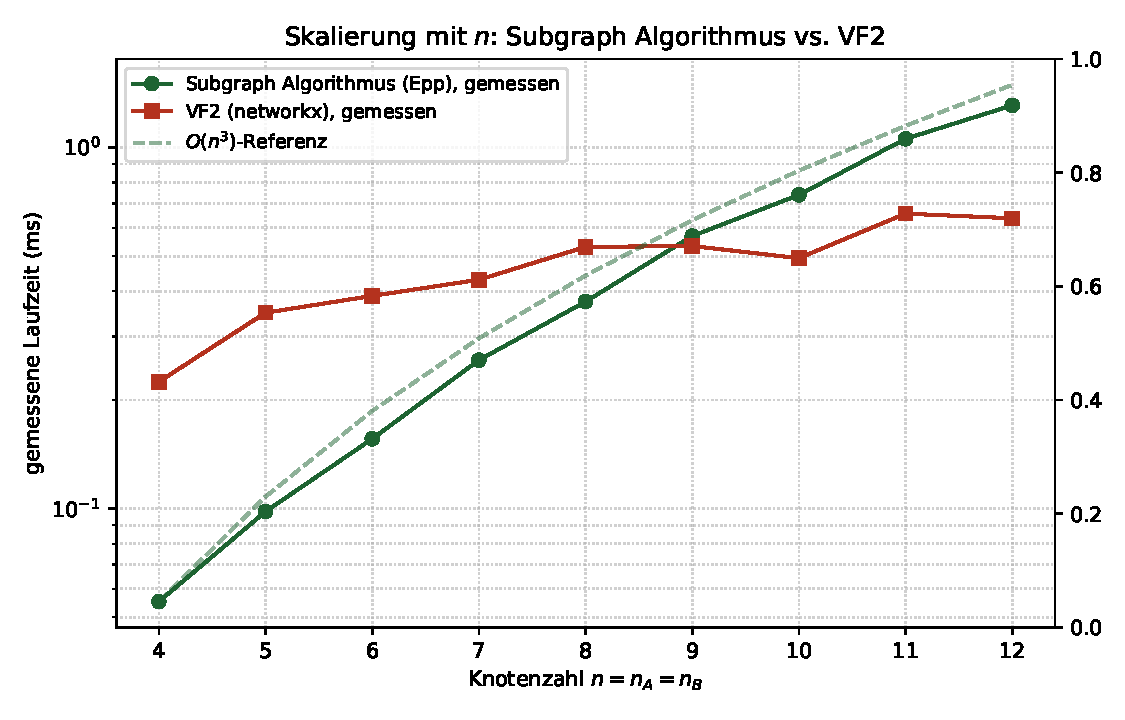
\includegraphics[width=0.75\textwidth]{plot7_scaling_comparison.pdf}
	\caption{Gemessene Laufzeit beider Verfahren bei gemeinsam wachsendem $n=n_A=n_B$ ($5$ Wiederholungen je $n$), zusammen mit einer auf den ersten Messpunkt skalierten $O(n^3)$-Referenzkurve für den Subgraph Algorithmus.}
	\label{fig:scaling_cmp}
\end{figure}

\textbf{Beschreibung:} Die gemessene Laufzeitkurve des Subgraph Algorithmus folgt der eingezeichneten $O(n^3)$-Referenz erkennbar enger als eine lineare oder quadratische Kurve es täte, was die in Satz~\ref{satz:laufzeit} bewiesene kubische Schranke empirisch stützt (für $n=4\to 12$, also Faktor $3$, wächst $T_{\text{Sub}}$ von $0{,}055\,$ms auf $1{,}309\,$ms, also um den Faktor $\approx 23{,}8$; $3^3=27$ liegt in derselben Größenordnung, die Abweichung erklärt sich durch den additiven $O(n^2)$-Signaturanteil, der bei kleinem $n$ relativ stärker wiegt). Die Laufzeit von VF2 wächst in diesem Bereich \emph{langsamer} als die des Subgraph Algorithmus (von $0{,}225\,$ms auf $0{,}637\,$ms, Faktor $\approx 2{,}8$ bei Verdreifachung von $n$) — ein empirischer Beleg dafür, dass die durchschnittliche Fallkomplexität von VF2 auf $G(n,0{,}3)$ deutlich unter der Worst-Case-Schranke $O(n!\,n)$ liegt, was mit den in \cite{he2008} berichteten durchschnittlichen Laufzeiten für VF2 und QuickSI auf zufälligen und realistischen Graphen konsistent ist (dort werden für Graphen mit $n\le 30$ ebenfalls Laufzeiten im Sub-Millisekunden- bis niedrigen Millisekundenbereich gemessen).

\subsection{Einordnung in effiziente Subgraph-Isomorphie-Verfahren}
\label{sec:literatur_cmp}

Tabelle~\ref{tab:literatur} fasst die in dieser Arbeit gemessenen Größenordnungen zusammen mit publizierten Charakterisierungen weiterer etablierter Algorithmen für (Teil-)Graphisomorphie und Subgraph-Suche. Die Tabelle dient nicht dem direkten Laufzeitvergleich auf identischer Hardware (die zitierten Arbeiten verwenden unterschiedliche Implementierungssprachen, Graphgrößen und Hardware-Generationen), sondern der \emph{komplexitätstheoretischen Einordnung}.

\begin{sidewaystable}
	\small
	%\scriptsize
	\centering
	\setlength{\tabcolsep}{3pt}
	\caption{Einordnung des Subgraph Algorithmus relativ zu etablierten Verfahren.}
	\begin{tabular}{>{\raggedright\arraybackslash}p{4.2cm}>{\raggedright\arraybackslash}p{4.8cm}>{\raggedright\arraybackslash}p{4.2cm}>{\raggedright\arraybackslash}p{6.4cm}}
		\toprule
		Verfahren & Worst-Case-Komplexität & Entschiedene Relation & Charakteristik \\
		\midrule
		Subgraph Algorithmus \cite{epp2026subgraph} & $O(n^3)$, bedingt optimal unter SETH \cite{abboud2015} & zyklische LCS-basierte Subsequenz-Relation $\preceq$ & polynomiell, eingabeunabhängige Schranke, geringe Varianz (Tabelle~\ref{tab:runtime}) \\
		Ullmann \cite{ullmann1976} & $O(n^{n})$ bzw.\ $O(n_A!\cdot n_B^{n_A})$ (naiv, mit Pruning praktisch geringer) & (Sub-)Graphisomorphie, Knotenbijektion $\phi$ & historischer Referenzalgorithmus, Backtracking mit Refinement \\
		VF2 \cite{cordella2004} & $O(n!\cdot n)$ Worst Case, oft sub-exponentiell in der Praxis & (Sub-)Graphisomorphie & Look\-ahead-Pruning (Schemata $0,1,2$); in dieser Arbeit gemessen, vgl.\ Tab.~\ref{tab:runtime} \\
		RI / RI-DS \cite{bonnici2013} & worst-case exponentiell, empirisch deutlich schneller als VF2 auf Bioinformatik-Graphen & (Sub-)Graphisomorphie & für biologische Netzwerke (PPI, Metabolismus) optimierte Knotenordnung \\
		QuickSI \cite{he2008} & worst-case exponentiell & Subgraph-Isomorphie (Pattern Matching) & Häufigkeits-basierte Kantenordnung, in \cite{he2008} ca.\ $10$--$1000\times$ schneller als naives Backtracking auf realen Graphdatenbanken \\
		GraphQL \cite{he2008} & worst-case exponentiell & Subgraph-Containment-Suche & nutzt Nachbarschafts-Signaturen zum Pruning, konzeptuell verwandt mit Pre-Filter aus Abschnitt~\ref{sec:prefilter} \\
		\bottomrule
	\end{tabular}
	\label{tab:literatur}
\end{sidewaystable}

Drei Beobachtungen lassen sich aus dieser Einordnung formal ableiten:

\begin{enumerate}
	\item \textbf{Komplexitätsklasse:} Der Subgraph Algorithmus ist das einzige der in Tabelle~\ref{tab:literatur} aufgeführten Verfahren mit einer \emph{unbedingten} polynomiellen Worst-Case-Schranke ($O(n^3)$, Satz~\ref{satz:laufzeit}). Alle übrigen Verfahren lösen das (im Allgemeinen NP-vollständige bzw.\ GI-vollständige) Subgraph-Isomorphie-Problem und besitzen daher worst-case zumindest superpolynomielle Schranken; ihre praktische Effizienz beruht auf Heuristiken (Pruning, Knoten\-ordnung, Nachbarschaftssignaturen), die im Average Case, aber nicht im Worst Case greifen. Dies ist konsistent mit der Tatsache, dass $\preceq$ (Definition~\ref{def:subgraphrelation_ref}) eine \emph{schwächere}, strukturell restriktivere Relation als die volle Subgraph-Isomorphie ist (vgl.\ Bemerkung zu Definition~\ref{def:vergleich}) — die polynomielle Schranke wird also durch eine Einschränkung des Relationsbegriffs erkauft, was formal die in \cite{epp2026subgraph} diskutierte SETH-basierte Optimalitätsanalyse motiviert.
	\item \textbf{Praktische Konsequenz für Satz~\ref{satz:pipeline}:} Da $T_{\text{Suche}}(N,C,n)=O(\log N+C)+O(C\cdot n^3)$ die Komplexität \emph{eines einzelnen} Subgraph-Vergleichs als $O(n^3)$ in die Pipeline einsetzt, wäre eine Substitution durch VF2, Ullmann, RI oder QuickSI formal nicht mit demselben Korollar (konstante Suchzeit unabhängig von $N$) vereinbar, da $O(n^3)$ durch eine worst-case-exponentielle Schranke ersetzt würde. Die empirisch hohe Average-Case-Effizienz von VF2/RI/QuickSI auf realistischen Graphen (Ergebnis~2, sowie \cite{he2008,bonnici2013}) bedeutet zwar, dass eine solche Substitution \emph{im Mittel} ähnlich performant sein könnte, jedoch ohne die formale Garantie aus Satz~\ref{satz:pipeline} — ein Datenbanksystem mit harten Latenzanforderungen (SLA) profitiert daher strukturell vom Subgraph Algorithmus.
	\item \textbf{Komplementarität statt Konkurrenz:} Die in \cite{bonnici2013,he2008} beschriebenen Optimierungen (Knotenordnung nach Seltenheit, Nachbarschaftssignaturen) sind \emph{orthogonal} zum Subgraph Algorithmus und könnten gemäß Abschnitt~\ref{sec:schluss} (z.\,B.\ R-Baum-Pre-Filter) auf die \emph{Pre-Filter-Stufe} der Gen-DB-Pipeline angewendet werden, während der eigentliche Vergleich der gefilterten Kandidaten durch den Subgraph Algorithmus mit garantierter $O(n^3)$-Schranke erfolgt. Insofern stehen die hier verglichenen Verfahren nicht in direkter Konkurrenz, sondern adressieren unterschiedliche Stufen derselben Pipeline (Kandidatenreduktion vs.\ finaler Strukturvergleich).
\end{enumerate}

\section{Experimentelle Untersuchung der Parallelisierung}
\label{sec:parallel}

Die bisherigen Abschnitte haben die Such-Pipeline von Gen-DB formal analysiert (Abschnitt~\ref{sec:pipeline}), an einer synthetischen Datenbank mit einer Million Netzwerken statistisch charakterisiert (Abschnitt~\ref{sec:evaluation}) und den Subgraph Algorithmus in Einzelvergleichen gegen VF2 gemessen (Abschnitt~\ref{sec:vergleich}). Offen geblieben ist die Frage, wie sich die \emph{gesamte} Suche verhält, wenn der dominierende Kostenterm $O(C\cdot n^3)$ aus Satz~\ref{satz:pipeline} auf mehrere Prozesse verteilt wird. Dieser Abschnitt beantwortet sie empirisch: Er beschreibt die in Gen-DB implementierte parallele Ausführung der Kandidatenvergleiche, den Aufbau eines reproduzierbaren Experiments mit $1$, $2$ und $3$ Worker-Prozessen und wertet die Messergebnisse anhand von vier Diagrammen und zwei Tabellen aus.

\subsection{Fragestellung und Hypothesen}
\label{sec:parallel_hyp}

Nach Satz~\ref{satz:pipeline} setzt sich die Suchzeit aus dem Pre-Filter $O(\log N + C)$ und den $C$ strukturellen Vergleichen $O(C\cdot n^3)$ zusammen. Da die Vergleiche für verschiedene Kandidaten voneinander unabhängig sind, lässt sich die Laufzeit einer Parallelisierung über $p$ Worker-Prozesse durch
\[
T_{\text{parallel}}(C,n,p) = O\!\left(\frac{C}{p}\cdot n^3\right) + O(n^3)
\]
modellieren. Das Experiment prüft drei daraus abgeleitete Hypothesen:

\begin{enumerate}
	\item[\textbf{H1}] Die Gesamtzeit einer Suche sinkt bei Verdopplung der Worker-Zahl von $1$ auf $2$ annähernd um den Faktor $2$, weil der parallelisierbare Vergleichsanteil die Laufzeit dominiert.
	\item[\textbf{H2}] Mehr Worker-Prozesse als logische Prozessoren der Maschine bringen keinen weiteren Gewinn, da die Vergleiche CPU-gebunden sind und keine zusätzliche Rechenkapazität entsteht.
	\item[\textbf{H3}] Die Suchzeit wächst, unabhängig von der Worker-Zahl, annähernd linear mit der Kandidatenzahl $C$, wie es der Term $O(C\cdot n^3)$ bei beschränktem $n\le 20$ erwarten lässt.
\end{enumerate}

\subsection{Implementierung der parallelen Suche}

Die Suche ist in der Funktion \texttt{search\_subgraph} des Moduls \texttt{crud} umgesetzt und läuft in drei Phasen. Zuerst liest eine einzige SQL-Abfrage alle Netzwerke, die die notwendigen Bedingungen $n_k \ge n_Q$ und $m_k \ge m_Q$ des Pre-Filters (Abschnitt~\ref{sec:prefilter}) erfüllen, zusammen mit ihren Adjazenzmatrizen. Danach übergibt \texttt{compare\_many} aus dem Modul \texttt{subgraph\_executor} die Matrizen an einen \texttt{ProcessPoolExecutor}, dessen Größe über die Konfigurationsvariable \texttt{SUBGRAPH\_MAX\_WORKERS} bestimmt wird. Jeder Worker-Prozess erzeugt genau eine Instanz des Subgraph Algorithmus und ruft für ein Paar aus Query $A$ und Kandidat $B$ die Methode \texttt{compare\_graphs(A, B)} auf. Weil der Algorithmus in reinem Python implementiert und CPU-gebunden ist, werden Prozesse statt Threads verwendet; der Global Interpreter Lock würde Threads sonst serialisieren. Um den Kommunikationsaufwand zwischen Hauptprozess und Workern zu verringern, werden die Kandidaten in Blöcken (\emph{Chunks}) von $256$ Vergleichen pro Task verteilt. Schließlich baut der Hauptprozess aus den Entscheidungen \texttt{keep\_B} und \texttt{equal\_keep\_*} die Trefferliste auf.

Zwei Eigenschaften dieser Implementierung sind für die Auswertung wichtig. Erstens enthält die aktuelle Fassung \emph{kein} Kandidatenlimit $K$; alle Kandidaten des Pre-Filters werden verglichen, sodass Satz~\ref{satz:korrektheit} mit $K=\infty$ gilt und die gemessenen Zeiten einer vollständigen Suche entsprechen. Zweitens sind nur die Vergleiche parallelisiert. Das Lesen der Kandidaten aus PostgreSQL, die Übertragung der Matrizen an die Worker und der Aufbau der Trefferliste laufen im Hauptprozess und bilden den seriellen Anteil der Suche.

\subsection{Versuchsaufbau}

Das Experiment wird durch das Skript \texttt{src/experiment\_search\_workers.py} gesteuert. Es wählt mit festem Seed zufällig Netzwerke aus der Datenbank und verwendet sie als Suchanfragen. Um Verzerrungen durch zu kleine Muster zu vermeiden, besitzen alle Queries mindestens $15$ Knoten. Für jede Worker-Anzahl werden \emph{dieselben} Anfragen in derselben Reihenfolge über \texttt{crud.search\_subgraph} ausgeführt, sodass die Zeiten als gepaarte Messungen direkt vergleichbar sind. Vor jeder Messreihe wird der Prozess-Pool neu erzeugt und alle Worker werden vorab gestartet, damit die Startzeit der Prozesse nicht in die Messung eingeht. Eine zusätzliche Aufwärmanfrage pro Worker-Anzahl wird verworfen, um Caching-Effekte der Datenbank auszugleichen. Gemessen wird die Wanduhrzeit der gesamten Funktion mit \texttt{time.perf\_counter()}; sie umfasst somit Datenbankabfrage, Vergleiche, Prozesskommunikation und Aufbau der Trefferliste. Nach jeder Anfrage schreibt das Skript die bisherigen Messwerte in eine JSON-Datei, sodass ein Abbruch keine Daten verliert.

\begin{table}[h]
	\centering
	\caption{Parameter und Umgebung des Experiments.}
	\label{tab:par_setup}
	\begin{tabular}{@{}ll@{}}
		\toprule
		Parameter & Wert \\
		\midrule
		Datenbank & $1.000.002$ Netzwerke (davon $333.500$ mit $n_k\ge 15$) \\
		Anzahl Anfragen & $6$ je Worker-Anzahl, identisch über alle Reihen \\
		Query-Auswahl & zufällig aus der Datenbank, $n_Q \ge 15$, Seed $42$ \\
		Worker-Anzahlen & $p\in\{1,2,3\}$ \\
		Aufwärmanfragen & $1$ je Worker-Anzahl (verworfen) \\
		Chunk-Größe & $256$ Vergleiche pro Task \\
		Kandidatenlimit & keines \\
		Rechner & $2$ logische Prozessoren, PostgreSQL~16 auf demselben System \\
		Software & Python~3.13, Linux \\
		\bottomrule
	\end{tabular}
\end{table}

Die ursprüngliche Voreinstellung des Skripts sieht $50$ Anfragen je Worker-Anzahl vor. Da eine einzelne Suche auf dem verwendeten Rechner bis zu rund $400$ Sekunden dauert, hätte diese Konfiguration mehrere Stunden benötigt; die Messreihe wurde deshalb auf $6$ Anfragen begrenzt (Aufruf: \texttt{python src/experiment\_search\_workers.py} \linebreak \texttt{--queries 6 --workers 1 2 3}). Die Folgen dieser Entscheidung für die Aussagekraft werden in Abschnitt~\ref{sec:par_grenzen} diskutiert.


\subsection{Metriken}

Für eine Worker-Anzahl $p$ bezeichne $T(p)$ die Summe der Antwortzeiten aller $Q=6$ Anfragen und $C_{\Sigma}=\sum_q C_q$ die Summe der Kandidatenzahlen.

\begin{definition}[Speedup, Effizienz, Durchsatz]
	\label{def:par_metriken}
	Der \emph{Speedup} ist $S(p)=T(1)/T(p)$, die \emph{parallele Effizienz} $E(p)=S(p)/p$. Der \emph{Durchsatz} ist $\Theta(p)=C_\Sigma/T(p)$ in Kandidaten pro Sekunde, und die \emph{Kosten pro Kandidat} sind $\kappa(p)=T(p)/C_\Sigma$.
\end{definition}

Aus dem Speedup lässt sich mit dem Gesetz von Amdahl der nicht parallelisierte Zeitanteil $f$ abschätzen. Gilt $T(p)=T(1)\bigl(f+\tfrac{1-f}{p}\bigr)$, so folgt
\[
f=\frac{1/S(p)-1/p}{1-1/p}.
\]
Diese Abschätzung ist nur sinnvoll, solange $p$ die Zahl der verfügbaren Prozessoren nicht übersteigt.

\subsection{Ergebnisse}

\subsubsection{Die untersuchten Anfragen}

Tabelle~\ref{tab:par_queries} zeigt die sechs ausgewählten Anfragen. Die Kandidatenzahl $C$ schwankt um mehr als den Faktor $5$, zwischen $62.064$ und $325.964$. Sie ergibt sich aus der Vorauswahl: Bei gleichverteilter Knotenzahl $n_k\in\{3,\dots,20\}$ besitzen $333.500$ der $1.000.002$ Netzwerke mindestens $15$ Knoten, und für Queries mit $15$ Knoten entscheidet nur noch die Kantenbedingung $m_k\ge m_Q$ über den Rest. Bei der Anfrage~5 mit $m_Q=56$ Kanten erfüllen $97{,}7\,\%$ dieser Netzwerke die Kantenbedingung, bei der Anfrage~1 mit $m_Q=68$ noch $82{,}6\,\%$. Die Anfragen~2 und~6 mit $19$ Knoten werden zusätzlich von der Knotenbedingung stark eingeschränkt, da nur Netzwerke mit $19$ oder $20$ Knoten in Frage kommen. Der Pre-Filter reduziert den Suchraum damit auf $6{,}2\,\%$ bis $32{,}6\,\%$ der Datenbank.

Die Trefferzahlen sind mit $1$ bis $7$ minimal. Da jede Query selbst ein Netzwerk der Datenbank ist und die Kandidatenmenge dieses Netzwerk enthält, ist zu erwarten, dass der einzelne Treffer der Anfragen mit genau einem Ergebnis dem Query-Netzwerk selbst entspricht. Netzwerke mit mindestens $15$ Knoten und der Kantendichte $p=0{,}3$ sind also in anderen Zufallsnetzwerken praktisch nie als Teilstruktur enthalten. Dieser Befund steht im Gegensatz zum Serverprotokoll in Abschnitt~\ref{sec:effiziente-suche}, bei dem nahezu alle Kandidaten Treffer waren; die Trefferquote hängt, wie dort bereits vermerkt, stark von der konkreten Query ab. Für die Laufzeitmessung ist das hier günstig, denn der Aufbau der Trefferliste im Hauptprozess ist vernachlässigbar, und die gemessene Zeit wird fast vollständig von Vorauswahl und Vergleichen bestimmt.

\begin{table}[h]
	\centering
	\small
	\caption{Eigenschaften der sechs Suchanfragen und Suchzeiten $t_p$ in Sekunden bei $p$ Workern.}
	\label{tab:par_queries}
	\begin{tabular}{@{}rrrrrrrrrr@{}}
		\toprule
		Nr. & Netzwerk-ID & $n_Q$ & $m_Q$ & $C$ & Treffer & $t_1$ & $t_2$ & $t_3$ & $S(2)$ \\
		\midrule
		1 & 654454 & 15 &  68 & 275.420 & 1 & 360{,}8 & 193{,}2 & 198{,}4 & 1{,}87 \\
		2 & 773650 & 19 & 107 &  62.064 & 1 &  70{,}0 &  36{,}7 &  40{,}6 & 1{,}91 \\
		3 & 432492 & 16 &  77 & 221.027 & 1 & 294{,}9 & 153{,}0 & 169{,}4 & 1{,}93 \\
		4 & 858614 & 15 &  70 & 263.668 & 3 & 354{,}9 & 185{,}8 & 209{,}2 & 1{,}91 \\
		5 & 438514 & 15 &  56 & 325.964 & 7 & 403{,}2 & 212{,}0 & 224{,}6 & 1{,}90 \\
		6 &  88827 & 19 &  95 & 100.911 & 1 & 120{,}4 &  62{,}4 &  65{,}4 & 1{,}93 \\
		\bottomrule
	\end{tabular}
\end{table}

\subsubsection{Gesamtzeit und Speedup}

\begin{figure}[!h]
	\centering
	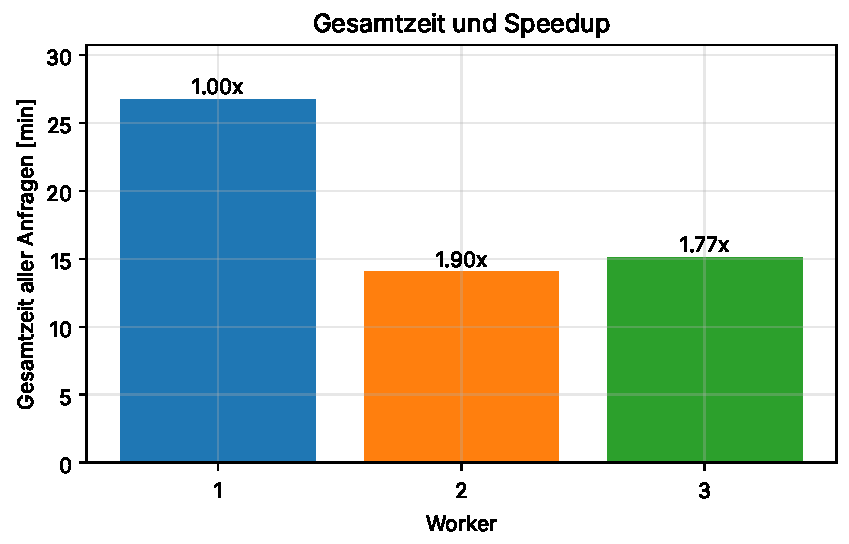
\includegraphics[width=0.75\textwidth]{../src/results/plot1_gesamtzeit_speedup.pdf}
	\caption{Gesamtzeit aller sechs Anfragen in Minuten für $1$, $2$ und $3$ Worker mit dem jeweiligen Speedup über den Balken.}
	\label{fig:par_gesamtzeit}
\end{figure}

Abbildung~\ref{fig:par_gesamtzeit} zeigt als Balkendiagramm die Summe der Antwortzeiten aller sechs Anfragen in Minuten, getrennt nach Worker-Anzahl. Über jedem Balken steht der Speedup relativ zur Messreihe mit einem Worker. Mit einem Worker benötigt die Suche zusammen $1604$ Sekunden, das sind rund $26{,}7$ Minuten. Mit zwei Workern sinkt dieser Wert auf $843$ Sekunden (rund $14{,}1$ Minuten), was einem Speedup von $S(2)=1{,}90$ und einer Effizienz von $E(2)=0{,}95$ entspricht. Der dritte Balken liegt bei $908$ Sekunden (rund $15{,}1$ Minuten) und damit \emph{über} dem Balken für zwei Worker; der Speedup fällt auf $S(3)=1{,}77$, die nominale Effizienz auf $E(3)=0{,}59$. Das Diagramm macht zwei Dinge sichtbar: den nahezu idealen Gewinn beim Übergang von einem auf zwei Worker und die leichte Verschlechterung durch einen dritten Worker, obwohl dessen Hinzunahme in einer idealen parallelen Maschine einen weiteren Gewinn bringen müsste.

Tabelle~\ref{tab:par_summary} fasst die Kennzahlen zusammen. Der Durchsatz steigt von $779$ auf $1482$ Kandidaten pro Sekunde und fällt mit drei Workern auf $1376$ zurück. Entsprechend sinken die Kosten pro Kandidat von $1{,}28$ auf $0{,}68$ Millisekunden und steigen mit drei Workern wieder auf $0{,}73$ Millisekunden. Aus $S(2)=1{,}90$ ergibt sich nach der Formel aus Definition~\ref{def:par_metriken} ein nicht parallelisierter Anteil von etwa $f\approx 5\,\%$. Dieser Wert fasst alle seriellen Anteile zusammen, darunter das Laden der bis zu $326.000$ Zeilen aus PostgreSQL, die Serialisierung der Matrizen für die Prozesskommunikation und den Aufbau der Trefferliste. Eine getrennte Zuordnung auf die einzelnen Phasen erlauben die vorliegenden Daten nicht, weil die Phasenzeiten im aktuellen Code nicht protokolliert werden.

\begin{table}[h]
	\centering
	\small
	\caption{Kennzahlen der Suche in Abhängigkeit von der Worker-Anzahl (jeweils $6$ Anfragen, $C_\Sigma = 1.249.054$ Kandidaten).}
	\label{tab:par_summary}
	\begin{tabular}{@{}rrrrrrrrr@{}}
		\toprule
		$p$ & $T(p)$ [s] & Mittel [s] & Median [s] & Max. [s] & $S(p)$ & $E(p)$ & $\Theta(p)$ [1/s] & $\kappa(p)$ [ms] \\
		\midrule
		1 & 1604 & 267{,}4 & 324{,}9 & 403{,}2 & 1{,}00 & 1{,}00 & 779  & 1{,}28 \\
		2 &  843 & 140{,}5 & 169{,}4 & 212{,}0 & 1{,}90 & 0{,}95 & 1482 & 0{,}68 \\
		3 &  908 & 151{,}3 & 183{,}9 & 224{,}6 & 1{,}77 & 0{,}59 & 1376 & 0{,}73 \\
		\bottomrule
	\end{tabular}
\end{table}

\subsubsection{Verteilung der Antwortzeiten}

\begin{figure}[!h]
	\centering
	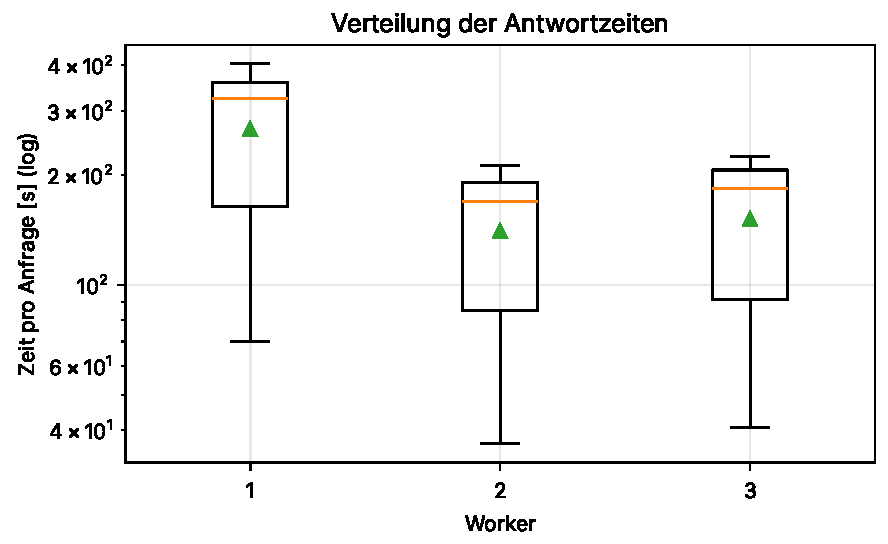
\includegraphics[width=0.75\textwidth]{../src/results/plot2_verteilung_antwortzeiten.pdf}
	\caption{Verteilung der Antwortzeit pro Anfrage als Boxplot mit logarithmischer Zeitachse und Mittelwert (Dreieck) für $1$, $2$ und $3$ Worker.}
	\label{fig:par_verteilung}
\end{figure}

Abbildung~\ref{fig:par_verteilung} stellt die Antwortzeiten der einzelnen Anfragen als Boxplots dar. Die Zeitachse ist logarithmisch, weil die Zeiten über mehr als eine Größenordnung streuen. Die Box umfasst das untere bis obere Quartil, die orange Linie markiert den Median, das grüne Dreieck den Mittelwert, und die Antennen reichen bis zur kleinsten bzw.\ größten Messung. Mit einem Worker liegen die Zeiten zwischen $70{,}0$ und $403{,}2$ Sekunden; das untere Quartil beträgt rund $164$ Sekunden, das obere rund $359$ Sekunden, der Median $324{,}9$ Sekunden und der Mittelwert $267{,}4$ Sekunden. Mit zwei Workern verschiebt sich die gesamte Verteilung nach unten: Die Zeiten reichen von $36{,}7$ bis $212{,}0$ Sekunden, die Quartile liegen bei rund $85$ und $191$ Sekunden, der Median bei $169{,}4$ und der Mittelwert bei $140{,}5$ Sekunden. Auf der logarithmischen Achse ist die Verschiebung für Minimum, Median und Maximum nahezu gleich groß, die Boxen haben also dieselbe Form. Das bedeutet, dass die Parallelisierung alle Anfragen unabhängig von ihrer Größe um etwa denselben Faktor beschleunigt und nicht nur besonders große oder kleine. Mit drei Workern liegt die Verteilung geringfügig oberhalb derjenigen mit zwei Workern (Median $183{,}9$ Sekunden, Maximum $224{,}6$ Sekunden), aber deutlich unterhalb der Verteilung mit einem Worker.

Der Median liegt bei jeder Worker-Anzahl über dem Mittelwert. Die Verteilung ist also linksschief: Wenige kurze Anfragen, nämlich die beiden Queries mit $19$ Knoten und vergleichsweise kleiner Kandidatenmenge, ziehen den Mittelwert herunter, während vier Anfragen mit großem Suchraum die Laufzeit bestimmen. Wegen der geringen Stichprobe von nur sechs Werten sind die Quartile grobe Orientierungswerte; das $95$-\%-Quantil, das das Skript ebenfalls ausgibt, ist bei sechs Werten identisch mit dem Maximum und wird deshalb hier nicht gesondert aufgeführt.

\subsubsection{Skalierung mit der Größe des Suchraums}

\begin{figure}[!h]
	\centering
	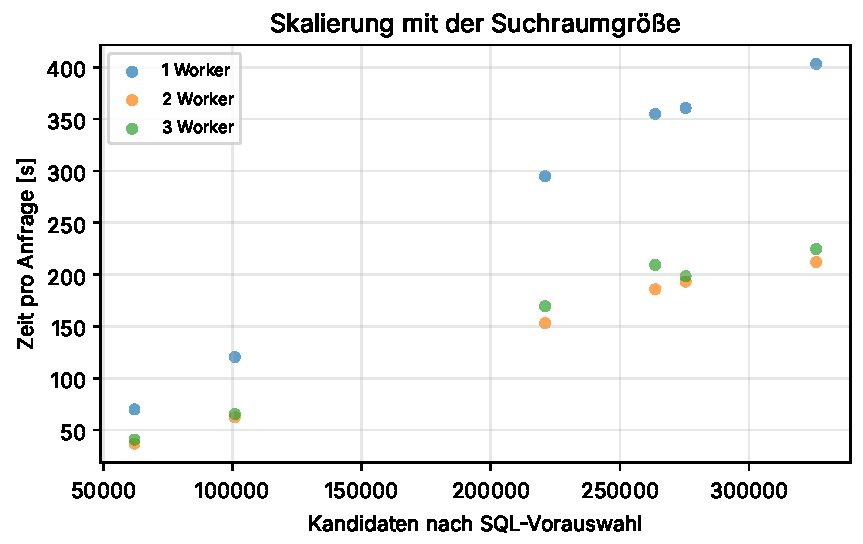
\includegraphics[width=0.75\textwidth]{../src/results/plot4_skalierung_suchraum.pdf}
	\caption{Streudiagramm der Antwortzeit gegen die Kandidatenzahl nach der SQL-Vorauswahl für $1$, $2$ und $3$ Worker.}
	\label{fig:par_skalierung}
\end{figure}

Abbildung~\ref{fig:par_skalierung} trägt für jede Anfrage und jede Worker-Anzahl die Antwortzeit gegen die Zahl der Kandidaten nach der SQL-Vorauswahl auf. Die Punkte jeder Worker-Anzahl liegen sehr nahe an einer Geraden, was Hypothese H3 stützt. Der Pearson-Korrelationskoeffizient zwischen $C$ und Antwortzeit beträgt $0{,}996$ für einen Worker, $0{,}996$ für zwei und $0{,}990$ für drei Worker. Die lineare Regression liefert für einen Worker eine Steigung von etwa $1{,}3$ Millisekunden je Kandidat, für zwei Worker etwa $0{,}70$ und für drei Worker etwa $0{,}75$ Millisekunden. Die Gerade für einen Worker verläuft also etwa doppelt so steil wie die Geraden für zwei und drei Worker, die ihrerseits fast aufeinander liegen, wobei die Punkte für drei Worker durchgehend leicht höher liegen. Die Parallelisierung ändert damit den Anstieg, nicht die Form des Zusammenhangs: Eine Verdopplung der Kandidatenzahl verdoppelt weiterhin die Suchzeit, nur mit etwa der halben Steigung.

Zugleich zeigt das Diagramm, dass der Zusammenhang nicht exakt proportional ist. Die Kosten pro Kandidat (Tabelle~\ref{tab:par_queries}, aus den Zeiten $t_1$ berechnet) betragen für die Anfragen mit $15$ oder $16$ Knoten zwischen $1{,}24$ und $1{,}35$ Millisekunden, für die beiden Anfragen mit $19$ Knoten dagegen nur $1{,}13$ und $1{,}19$ Millisekunden. Die Regressionsgerade besitzt entsprechend einen negativen Achsenabschnitt. Aus der Kubikschranke $O(n^3)$ ließe sich für Queries mit mehr Knoten ein höherer, nicht ein niedrigerer Aufwand pro Vergleich erwarten. Die Schranke ist aber eine Worst-Case-Abschätzung für den Vergleich; die Messung zeigt, dass der tatsächliche Aufwand auf diesen Daten auch von anderen Faktoren abhängt, etwa davon, wie früh ein Vergleich entschieden werden kann. Eine belastbare Erklärung erlaubt die vorliegende Messreihe nicht, weil dafür Zeiten einzelner Vergleiche in Abhängigkeit von $n_Q$ und $n_k$ erhoben werden müssten.

\subsubsection{Dieselben Anfragen im direkten Vergleich}

\begin{figure}[!h]
	\centering
	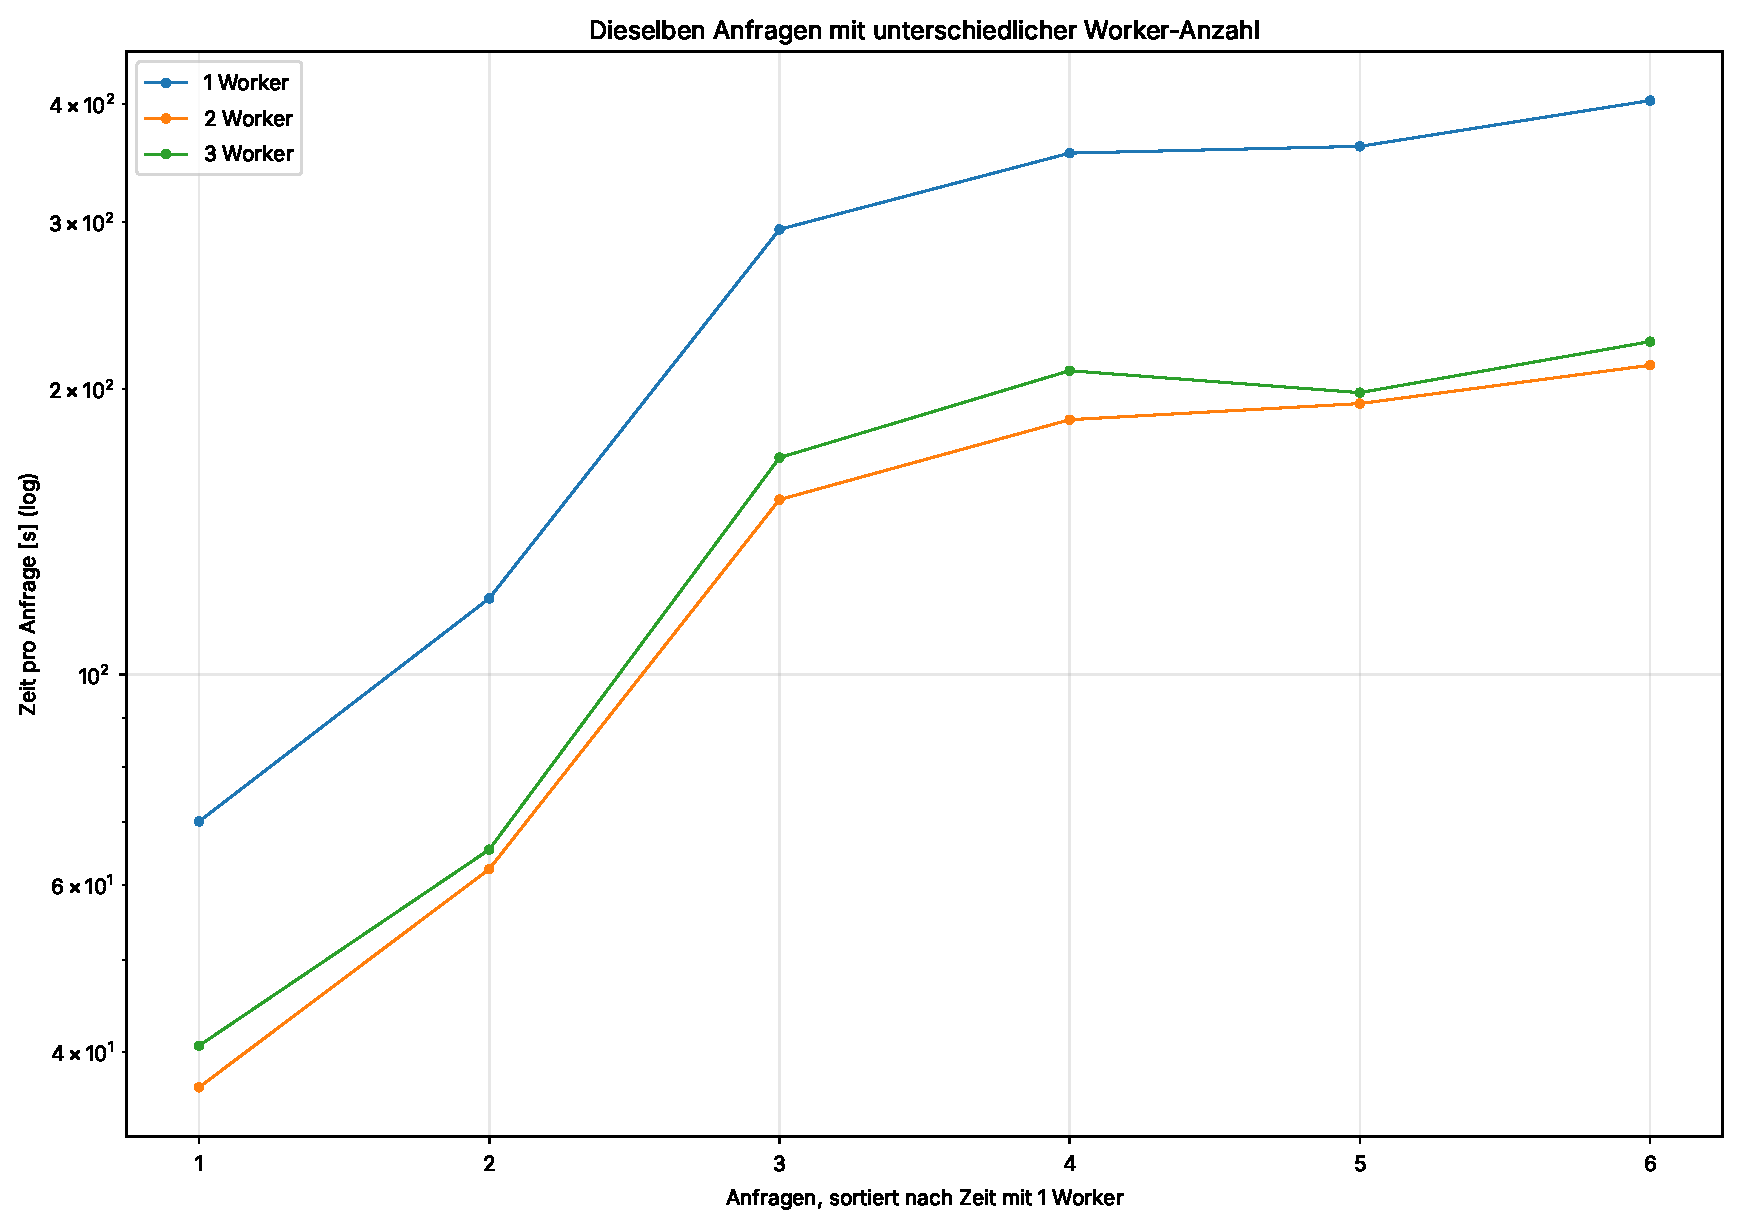
\includegraphics[width=0.65\textwidth]{../src/results/plot5_gleiche_anfragen_je_worker.pdf}
	\caption{Antwortzeit jeder einzelnen Anfrage bei $1$, $2$ und $3$ Workern, sortiert nach der Zeit mit einem Worker, logarithmische Zeitachse.}
	\label{fig:par_gleiche}
\end{figure}

Abbildung~\ref{fig:par_gleiche} ordnet die Anfragen auf der horizontalen Achse nach ihrer Laufzeit mit einem Worker und zeichnet für jede Worker-Anzahl einen Linienzug durch die zugehörigen Zeiten. Weil dieselben Anfragen in allen drei Messreihen verwendet wurden, zeigt jeder vertikale Schnitt dieselbe Anfrage unter drei Bedingungen. Die Linie für einen Worker liegt an jeder Stelle oberhalb der beiden anderen, die Linien für zwei und drei Worker verlaufen nahezu parallel zueinander, wobei die Linie für drei Worker für alle sechs Anfragen über der für zwei Worker liegt. Auf der logarithmischen Achse entspricht ein konstanter Faktor einem konstanten vertikalen Abstand; dass die Abstände zwischen den Linien über alle Positionen annähernd gleich bleiben, bestätigt, dass die Beschleunigung von der Größe der Anfrage weitgehend unabhängig ist. Der Speedup $S(2)$ liegt für die einzelnen Anfragen zwischen $1{,}87$ und $1{,}93$ (Tabelle~\ref{tab:par_queries}), der Speedup $S(3)$ zwischen $1{,}70$ und $1{,}84$. Diese enge Streuung ist ein Hinweis, dass der Gesamtwert $S(2)=1{,}90$ keine Folge einzelner Ausreißer ist. Besonders deutlich ist der Sprung von der zweiten zur dritten Position: Die Anfrage~3 ist mit $221.027$ Kandidaten wesentlich aufwendiger als die Anfrage~6 mit $100.911$ Kandidaten, und der Abstand zwischen den Linien bleibt trotzdem derselbe.

\subsection{Diskussion}

\paragraph{Hypothese H1.} Der Übergang von einem auf zwei Worker liefert einen Speedup von $1{,}90$ bei einer Effizienz von $95\,\%$, und alle sechs Anfragen liegen zwischen $1{,}87$ und $1{,}93$. Die Hypothese ist damit auf dem untersuchten Rechner bestätigt: Der parallelisierbare Vergleichsanteil dominiert die Laufzeit, und der serielle Anteil von etwa $5\,\%$ (Laden der Kandidaten, Prozesskommunikation, Aufbau der Trefferliste) begrenzt den Gewinn nur geringfügig. Die Messung stützt das in Abschnitt~\ref{sec:parallel_hyp} angegebene Modell $T_{\text{parallel}}=O(\frac{C}{p}n^3)+O(n^3)$, wobei der additive Term nur den langsamsten Einzelvergleich erfasst. Die Messung zeigt, dass zusätzlich ein mit $C$ wachsender serieller Anteil existiert, der in diesem Modell nicht abgebildet ist. Er fällt bei $p=2$ kaum ins Gewicht, würde bei größerem $p$ aber nach dem Gesetz von Amdahl zunehmend den erreichbaren Speedup bestimmen.

\paragraph{Hypothese H2.} Mit drei Workern auf einem Rechner mit zwei logischen Prozessoren steigt die Gesamtzeit um rund $7{,}7\,\%$ gegenüber zwei Workern, und der Speedup fällt von $1{,}90$ auf $1{,}77$. Auch diese Hypothese wird bestätigt. Die Vergleiche sind rein rechengebunden; ein dritter Prozess erzeugt keine zusätzliche Rechenkapazität, sondern konkurriert mit den anderen Prozessen um dieselben zwei Prozessoren und verursacht zusätzliche Kontextwechsel. Hinzu kommt, dass auch der Hauptprozess, der die Ergebnisse einsammelt, und der PostgreSQL-Server auf demselben Rechner Rechenzeit benötigen. Welchen Anteil diese Effekte jeweils haben, lässt sich aus den Daten nicht trennen. Die Beobachtung lässt sich aber unmittelbar in eine Konfigurationsempfehlung übersetzen: Die Zahl der Worker sollte die Zahl der verfügbaren logischen Prozessoren nicht überschreiten. Die mitgelieferte \texttt{.env}-Datei setzt \texttt{SUBGRAPH\_MAX\_WORKERS=14}; dieser Wert ist nur auf einem Rechner mit mindestens vierzehn logischen Prozessoren sinnvoll und sollte für andere Systeme angepasst werden.

\paragraph{Hypothese H3.} Die Antwortzeit hängt mit einem Korrelationskoeffizienten von mindestens $0{,}99$ linear von der Kandidatenzahl ab. Das stimmt mit dem Term $O(C\cdot n^3)$ aus Satz~\ref{satz:pipeline} bei beschränktem $n$ überein. Die Abweichungen in den Kosten pro Kandidat zeigen allerdings, dass die Konstante nicht allein durch die Knotenzahl bestimmt wird (siehe oben).

\paragraph{Bedeutung für das Korollar zur Datenbankgröße.} Das Korollar zu Satz~\ref{satz:pipeline} behauptet eine von $N$ unabhängige Suchzeit, sofern die Kandidatenzahl durch ein Limit $K$ beschränkt ist. Das Experiment läuft bewusst ohne Limit und zeigt die Kehrseite: Bei $N\approx 10^6$ bleiben je nach Query bis zu $32{,}6\,\%$ der Datenbank als Kandidaten übrig, und die Suchzeit steigt dann proportional zu $C$ auf bis zu $403$ Sekunden mit einem und $212$ Sekunden mit zwei Workern. Ohne Limit wächst $C$ bei fester Selektivität des Pre-Filters linear mit $N$, und damit auch die Suchzeit. Die Parallelisierung verkleinert den Anstieg um etwa den Faktor $p$, hebt die Abhängigkeit von $N$ aber nicht auf. Wer harte Latenzgrenzen einhalten will, braucht deshalb weiterhin einen schärferen Pre-Filter (etwa den in Abschnitt~\ref{sec:schluss} diskutierten mehrdimensionalen Index) oder ein Kandidatenlimit mit den dort beschriebenen Einbußen bei der Vollständigkeit; die Parallelisierung ergänzt diese Maßnahmen, ersetzt sie aber nicht.

\subsection{Grenzen der Untersuchung}
\label{sec:par_grenzen}

Die Ergebnisse sind als erste empirische Einordnung zu lesen und aus folgenden Gründen nicht ohne Weiteres verallgemeinerbar.

\begin{itemize}
	\item \textbf{Kleine Stichprobe.} Mit sechs Anfragen und einer Messung je Anfrage und Worker-Anzahl lassen sich keine Standardabweichungen über Wiederholungen und keine Signifikanztests angeben. Dass die Speedups der einzelnen Anfragen eng beieinander liegen, spricht für stabile Verhältnisse, ersetzt aber keine Wiederholungsmessungen. Die ursprünglich vorgesehenen $50$ Anfragen sollten auf einem Rechner mit mehr Prozessoren nachgeholt werden.
	\item \textbf{Zwei logische Prozessoren.} Aussagen für $p>2$ beschränken sich auf die Überbelegung; das Skalierungsverhalten bei vier, acht oder vierzehn echten Prozessoren, insbesondere der Einfluss des seriellen Anteils, wird nicht gemessen. Die Abschätzung $f\approx 5\,\%$ beruht auf einem einzigen Messpunkt.
	\item \textbf{Gemeinsam genutzter Rechner.} Datenbank, Hauptprozess und Worker teilen sich dieselben Prozessoren. Auf einem System mit separatem Datenbankserver würde sich der serielle Anteil anders verhalten. Die Absolutwerte sind außerdem nicht mit dem Serverprotokoll aus Abschnitt~\ref{sec:effiziente-suche} vergleichbar, das auf einem anderen System entstand.
	\item \textbf{Keine Phasenzerlegung.} Der Code protokolliert die Zeiten für Laden, Vergleichen und Trefferaufbau nicht, weshalb das Diagramm „Zeit je Phase“ des Skripts leer bleibt und dieser Abschnitt auf seine Wiedergabe verzichtet. Der serielle Anteil kann daher nur indirekt aus dem Speedup abgeschätzt werden.
	\item \textbf{Eine synthetische Graphenfamilie.} Alle Netzwerke stammen aus dem Erdős–Rényi-Modell mit $p=0{,}3$; für reale biologische Netzwerke mit anderer Dichte und Struktur können Kandidatenzahlen, Trefferquoten und Kosten pro Vergleich abweichen.
	\item \textbf{Treffer von Query und Kandidat.} Da die Queries aus der Datenbank stammen, enthält jede Kandidatenmenge das Query-Netzwerk selbst. Das ist für die Laufzeitmessung unerheblich, spricht aber gegen eine Interpretation der Trefferzahlen als allgemeine Trefferquote.
\end{itemize}

\subsection{Zwischenfazit}

Die parallele Ausführung der Kandidatenvergleiche über einen Prozess-Pool beschleunigt die Suche in Gen-DB auf dem untersuchten Rechner mit zwei logischen Prozessoren um den Faktor $1{,}90$ (Effizienz $95\,\%$); der Gewinn ist für alle sechs Anfragen nahezu gleich. Ein dritter Worker verschlechtert die Zeit um rund $8\,\%$, da keine zusätzliche Rechenkapazität zur Verfügung steht. Die Suchzeit wächst unabhängig von der Worker-Zahl linear mit der Kandidatenzahl und erreicht ohne Kandidatenlimit bei großen Suchräumen mehrere Minuten, sodass die Parallelisierung die Antwortzeit um einen konstanten Faktor senkt, aber die Notwendigkeit eines selektiveren Pre-Filters oder eines Kandidatenlimits nicht beseitigt. Für die Praxis folgt daraus die Empfehlung, die Worker-Anzahl an die Zahl der logischen Prozessoren anzupassen. Die offene Frage, wie weit sich der Gewinn auf Rechnern mit deutlich mehr Prozessoren fortsetzt, soll eine Wiederholung der Messreihe mit der vollen Anfragezahl klären.

\section{Experimenteller Vergleich Python und C++}
\label{sec:backends}

Die vorangegangene Untersuchung hat gezeigt, dass sich die Suchzeit durch mehrere Worker-Prozesse deutlich reduzieren lässt. Sie beantwortet jedoch nicht, ob auch der einzelne Subgraph-Vergleich schneller ausgeführt werden kann. Dieses Kapitel untersucht deshalb die C++17-Implementierung aus dem Projekt \texttt{csubgraph}, die als Library direkt im langlebigen Gen-DB-Worker aufgerufen wird. Ein früherer Messlauf über die C++-CLI hatte den Prozessstart und JSON-Austausch als erhebliche Kostenquelle sichtbar gemacht; seine Messwerte sind von den hier ausgewerteten Library-Werten zu trennen.

Das Experiment vergleicht auf zwei Ebenen. Der Mikrobenchmark misst direkte Python-Aufrufe und Funktionsaufrufe der C++-Library auf denselben Graphpaaren sowie die Kosten eines trivialen Library-Aufrufs. Die Ende-zu-Ende-Messung vergleicht die vollständige Gen-DB-Suche für identische Queries, Kandidatenmengen und Worker-Zahlen. So werden sowohl der Effekt auf den Einzelvergleich als auch der praktisch relevante Einfluss auf die Antwortzeit erfasst. Die abgeschlossene Messreihe vom 7. Oktober 2026 umfasst sechs Suchanfragen; beide Backends lieferten identische Treffer-IDs und es traten keine fehlgeschlagenen Vergleiche auf.

\subsection{Motivation und Fragestellung}
\label{sec:backend_motivation}

Der Algorithmus bildet den rechenintensiven Teil der Kandidatenprüfung in Gen-DB. Nach dem datenbankseitigen Pre-Filter wird jedes verbliebene Netzwerk mit der Query verglichen. Bei mehr als einer Million Kandidaten kann selbst eine geringe Zeitersparnis pro Paar einen großen Unterschied für die gesamte Suche bedeuten. Zugleich unterscheidet sich der Aufwand eines Algorithmusaufrufs von dem Aufwand, den die umgebende Anwendung tatsächlich misst: Daten müssen in das jeweilige Format überführt, an den ausführenden Prozess übergeben und das Ergebnis muss zurücktransportiert und interpretiert werden.

Das Experiment untersucht daher folgende Fragen:

\begin{enumerate}
	\item Wie unterscheiden sich direkte Aufrufe der Python-Implementierung und der C++-Library für dieselben Graphpaare?
	\item Wie groß sind die Übergabekosten der Library im Verhältnis zur Laufzeit eines trivialen Vergleichs?
	\item Führt der Einsatz der C++-Library bei identischen Queries, Kandidaten und Worker-Zahlen zu einer kürzeren Ende-zu-Ende-Suchzeit?
	\item Liefern beide Backends für dieselben Queries dieselben Treffer-IDs, und treten bei einem Backend fehlgeschlagene Einzelvergleiche auf?
\end{enumerate}

Daraus ergeben sich vier Hypothesen. \textbf{H1:} Ein direkter Aufruf des nativen Algorithmuskerns benötigt weniger Zeit als ein Python-Aufruf. \textbf{H2:} Der Vorteil bleibt nach Einbeziehung der Library-Schnittstelle groß genug, um die vollständige Gen-DB-Suche zu beschleunigen. \textbf{H3:} Beide Implementierungen liefern für alle Queries dieselben Suchtreffer. \textbf{H4:} Die Kosten der Library-Schnittstelle sind im Verhältnis zur Rechenzeit klein, während ein Prozess-pro-Vergleich-CLI-Aufruf erheblichen Zusatzaufwand verursachen kann. Der abgeschlossene Mikrobenchmark und Suchlauf liefern für H1 bis H3 direkte Messwerte; H4 wird durch die Library-Aufrufkosten und den separat dokumentierten früheren CLI-Mikrobenchmark eingeordnet.

\subsection{Implementierungen und Ausführungspfade}
\label{sec:backend_implementierungen}

Beide Backends führen denselben Subgraph Algorithmus aus. Wie in Abschnitt~\ref{sec:grundlagen} beschrieben, vergleicht dieser die aus den Adjazenzmatrizen abgeleiteten Zeilenkomponenten unter zyklischen Rotationen und entscheidet anhand einer dynamischen Übereinstimmungsprüfung über die Relation der Graphen. Die Python-Implementierung wird über \texttt{Subgraph().compare\_graphs(A, B)} aufgerufen. Für C++ wird die statische Bibliothek \texttt{libsubgraphlib.a} mit einem C-Wrapper zu einer DLL gelinkt und über \texttt{ctypes} angesprochen. Die DLL wird einmal pro Worker-Prozess geladen; ein Vergleich erfolgt danach als direkter Funktionsaufruf.

Beide Varianten laufen in einem langlebigen \texttt{ProcessPoolExecutor} mit zwei Workern und erhalten Kandidaten blockweise mit Chunk-Größe $256$. Anders als bei der früheren CLI-Integration wird für C++ weder je Kandidat ein weiterer Prozess gestartet noch werden Matrizen und Resultate über JSON-Pipes serialisiert. Der einmalige Bau und das Linken des Wrappers finden vor dem Start des Pools statt und sind nicht Teil der gemessenen Suchzeit. Der Mikrobenchmark misst den direkten Funktionspfad einschließlich der Übergabe der Arrays an den Wrapper und vergleicht somit reale Aufrufpfade, nicht abstrakt bereinigte Sprachlaufzeiten.

Das Experiment kontrolliert, dass in Haupt- und Worker-Prozessen tatsächlich das jeweils angeforderte Backend aktiv ist, zählt fehlgeschlagene Vergleiche und gleicht für jede Anfrage die gefundenen Netzwerk-IDs ab. Damit lässt sich neben der Laufzeit auch die Ergebniskonformität der beiden Implementierungen beurteilen.

\subsection{Versuchsaufbau}
\label{sec:backend_versuchsaufbau}

Das Experiment wird durch \texttt{src/experiment\_search\_backends.py} gesteuert. Es verwendet dieselbe Datenbank für beide Implementierungen, wählt mit Seed $42$ sechs Netzwerke als Queries und setzt die Untergrenze auf $15$ Knoten. Beide Backends werden mit zwei Workern und in derselben Reihenfolge ausgewählten Queries ausgeführt. Vor jeder Messreihe wird eine Aufwärmanfrage verworfen. Die JSON-Datei wird nach jeder abgeschlossenen Anfrage aktualisiert, damit ein Abbruch die bis dahin geschriebenen Messwerte nicht verliert. Zusätzlich prüft das Skript die Treffer-IDs, kontrolliert die tatsächlich in den Worker-Prozessen aktive Implementierung und zählt fehlgeschlagene Einzelvergleiche.

Der Mikrobenchmark wird ohne Datenbank ausgeführt. Mit Seed $42$ werden $200$ Zufallspaare erzeugt. Die erste Matrix besitzt zwischen $15$ und $19$ Knoten, die zweite $20$ Knoten; jede mögliche gerichtete Kante wird mit Wahrscheinlichkeit $0{,}3$ gewählt. Beide Backends verarbeiten dieselben Paare. Für C++ wird außerdem der direkte Bibliotheksaufruf mit zwei trivialen $1\times1$-Matrizen gemessen. Dieser Wert nähert die Kosten von Array-Marshalling und Funktionsübergabe an, nicht jedoch alle denkbaren Aufwände größerer Matrizen.

\begin{table}[h]
	\centering
	\small
	\caption{Versuchsparameter und Umgebung des Backend-Vergleichs.}
	\label{tab:backend_setup}
	\begin{tabular}{@{}ll@{}}
		\toprule
		Parameter & Wert \\
		\midrule
		Backend-Reihenfolge & Python, anschließend C++-Library \\
		Worker je Backend & $2$ \\
		Queries & $6$, zufällig aus der Datenbank, Seed $42$ \\
		Mindestgröße der Queries & $15$ Knoten \\
		Aufwärmung & eine verworfene Suche je Backend \\
		Mikrobenchmark & $200$ Zufallspaare, Seed $42$ \\
		Knotenzahl Mikrobenchmark & $n_A\in\{15,\ldots,19\}$, $n_B=20$ \\
		Kantenwahrscheinlichkeit & $0{,}3$ \\
		Library-Referenz & $200$ Aufrufe mit trivialen $1\times1$-Matrizen \\
		Betriebssystem & Windows 11 \\
		Python & $3.14.8$ \\
		Logische Prozessoren & $4$ \\
		C++-Bibliothek & \texttt{libsubgraphlib.a}, Wrapper-DLL über \texttt{ctypes} \\
		\bottomrule
	\end{tabular}
\end{table}

Die volle Suche misst mit \texttt{time.perf\_counter()} die Wanduhrzeit von \texttt{crud.search\_subgraph()}. Sie umfasst damit die Datenbankabfrage, die Vergleichsphase, die Kommunikation mit den Worker-Prozessen und den Aufbau der Trefferliste. Zusätzlich werden die in \texttt{compare\_many} verbrauchte Zeit und der als Differenz berechnete Rest der Suche protokolliert. Für jede Query werden Knotenzahl, Kantenzahl, Zahl der Kandidaten nach SQL-Vorauswahl, Trefferzahl und Fehlerzahl festgehalten. Die Summe der Antwortzeiten je Backend erlaubt den direkten Gesamtvergleich; die jeweiligen Treffer-IDs dienen dem Abgleich der funktionalen Ergebnisse.

\subsection{Metriken}
\label{sec:backend_metriken}

Für dieselbe Query $q$ bezeichne $t_{\mathrm{Py},q}$ die gemessene Suchzeit mit der Python-Implementierung und $t_{\mathrm{C++},q}$ die Zeit mit der C++-Library. Der relative Such-Speedup ist
\[
	S_{\mathrm{C++}} = \frac{\sum_q t_{\mathrm{Py},q}}{\sum_q t_{\mathrm{C++},q}}.
\]
Ein Wert größer als $1$ bedeutet, dass die C++-Library in der gemessenen Gen-DB-Ausführung schneller war; ein Wert kleiner als $1$ bedeutet eine langsamere Suche. Der Quotient vergleicht die gesamte Integration und nicht allein den nativen Algorithmuskern. Ergänzend misst das Skript den Kandidatendurchsatz $\Theta=C_{\Sigma}/T$ und die Kosten pro Kandidat $\kappa=T/C_{\Sigma}$, wobei $C_{\Sigma}$ die Summe der Kandidatenzahlen und $T$ die Summe der Antwortzeiten eines Backends ist.

Die funktionale Übereinstimmung wird pro Query über die sortierten Listen der gefundenen Netzwerk-IDs geprüft. Zusätzlich vergleicht das Skript die erwartete Backend-Kennung in Haupt- und Worker-Prozessen und protokolliert fehlgeschlagene Vergleiche. Dadurch ist ein stiller Rückfall auf Python nicht mit einem erfolgreichen C++-Lauf zu verwechseln. Der Mikrobenchmark beantwortet eine andere Frage als der Such-Speedup: Er isoliert den wiederholten direkten Funktionsaufruf im Hauptprozess; die Ende-zu-Ende-Messung umfasst zusätzlich Datenbankzugriff, Worker-Kommunikation und Ergebnisaufbau.

\subsection{Ergebnisse der abgeschlossenen Messreihe}
\label{sec:backend_zwischenstand}

Die ausgewertete Datei \texttt{search\_backends\_20261007\_104804.json} ist mit \texttt{complete=true} markiert. Sechs Queries mit mindestens $15$ Knoten wurden bei zwei Workern in beiden Backends ausgeführt; zusammen durchlief jede Implementierung exakt $931.899$ Kandidaten. Tabelle~\ref{tab:backend_summary} fasst die Such- und Kalibrierungskennzahlen zusammen. Die Laufzeiten pro Query in Tabelle~\ref{tab:backend_queries} zeigen ergänzend, dass der beobachtete Gewinn nicht von einer einzelnen Anfrage getragen wird.

% Automatisch erzeugt von src/experiment_search_backends.py -- nicht von Hand ändern.
% Messlauf: 2026-10-07T10:48:05, Seed 42
\begin{table}[h]
	\centering
	\small
	\caption{Kennzahlen der Suche je Implementierung (jeweils $6$ Anfragen, $C_\Sigma = 931.899$ Kandidaten, Speedup $S$ relativ zu Python).}
	\label{tab:backend_summary}
	\begin{tabular}{@{}lrrrrrrrrr@{}}
		\toprule
		Variante & $p$ & $T$ [s] & Mittel [s] & Median [s] & Max. [s] & $S$ & $\Theta$ [1/s] & $\kappa$ [ms] & seriell [\%] \\
		\midrule
		Python & 2 & 1.180 & 196{,}7 & 145{,}3 & 379{,}2 & 1{,}00 & 790 & 1{,}267 & 11{,}6 \\
		C++ & 2 & 186 & 30{,}9 & 26{,}2 & 63{,}6 & 6{,}36 & 5.020 & 0{,}199 & 66{,}7 \\
		\bottomrule
	\end{tabular}
\end{table}

\begin{table}[h]
	\centering
	\small
	\caption{Zeit je Einzelvergleich im Hauptprozess (200 Zufallspaare mit $n_A\in\{15,\dots,19\}$, $n_B=20$, Kantenwahrscheinlichkeit $0{,}3$).}
	\label{tab:backend_calibration}
	\begin{tabular}{@{}lrrr@{}}
		\toprule
		Messung & Median [ms] & Mittel [ms] & Max. [ms] \\
		\midrule
		Python, Einzelvergleich & 2{,}793 & 2{,}694 & 3{,}703 \\
		C++ (Bibliothek), Einzelvergleich & 0{,}068 & 0{,}074 & 0{,}331 \\
		C++ (Bibliothek), trivialer $1\times1$-Aufruf & 0{,}018 & 0{,}018 & 0{,}073 \\
		\bottomrule
	\end{tabular}
\end{table}


\begin{table}[!htbp]
	\centering
	\small
	\caption{Antwortzeiten und Ergebnisse der sechs identischen Suchanfragen mit jeweils zwei Workern.}
	\label{tab:backend_queries}
	\begin{tabular}{@{}rrrrrrrrr@{}}
		\toprule
		Nr. & Netzwerk-ID & $n_Q$ & $m_Q$ & Kandidaten & Treffer & Python [s] & C++ [s] & Speedup \\
		\midrule
		1 & 654.525 & 18 & 106 & 69.173 & 1 & 97{,}39 & 11{,}11 & $8{,}76\times$ \\
		2 & 773.692 & 19 & 104 & 74.482 & 1 & 85{,}22 & 12{,}33 & $6{,}91\times$ \\
		3 & 432.763 & 15 &  63 & 302.555 & 1 & 379{,}18 & 51{,}08 & $7{,}42\times$ \\
		4 & 858.300 & 20 & 110 & 38.496 & 1 & 50{,}66 & 7{,}31 & $6{,}93\times$ \\
		5 & 438.602 & 15 &  66 & 287.228 & 1 & 374{,}62 & 63{,}62 & $5{,}89\times$ \\
		6 & 89.411 & 18 &  83 & 159.965 & 1 & 193{,}21 & 40{,}16 & $4{,}81\times$ \\
		\bottomrule
	\end{tabular}
\end{table}

Die Python-Suche benötigte insgesamt $1.180{,}28$ Sekunden, also $19$ Minuten und $40$ Sekunden; die C++-Library benötigte $185{,}62$ Sekunden, rund $3$ Minuten und $6$ Sekunden. Der aggregierte Speedup beträgt damit $6{,}36\times$ und die Suchzeit sinkt um etwa $84{,}3\,\%$. Der Geschwindigkeitsgewinn ist für jede der sechs Einzelanfragen sichtbar: Die individuellen Speedups reichen von $4{,}81\times$ bis $8{,}76\times$. Ihre Streuung macht zugleich deutlich, dass ein einzelner Gesamtfaktor keine für jede Query identische Beschleunigung verspricht.

Die Query mit den meisten Kandidaten ($302.555$) benötigt mit Python $379{,}18$ Sekunden und mit C++ $51{,}08$ Sekunden; die zweite Anfrage mit annähernd ebenso vielen Kandidaten zeigt mit $287.228$ Kandidaten und $374{,}62$ beziehungsweise $63{,}62$ Sekunden ein ähnliches, aber etwas kleineres Verhältnis. Die Query mit den wenigsten Kandidaten ($38.496$) ist in beiden Backends die schnellste. Die Messreihe passt damit zur erwarteten Abhängigkeit von der Größe des Suchraums. Wegen nur sechs Queries und variierender Knotenzahlen ist sie jedoch keine kontrollierte Regression, aus der eine allgemeingültige Zeit pro Kandidat abgeleitet werden könnte.

\begin{figure}[!h]
	\centering
	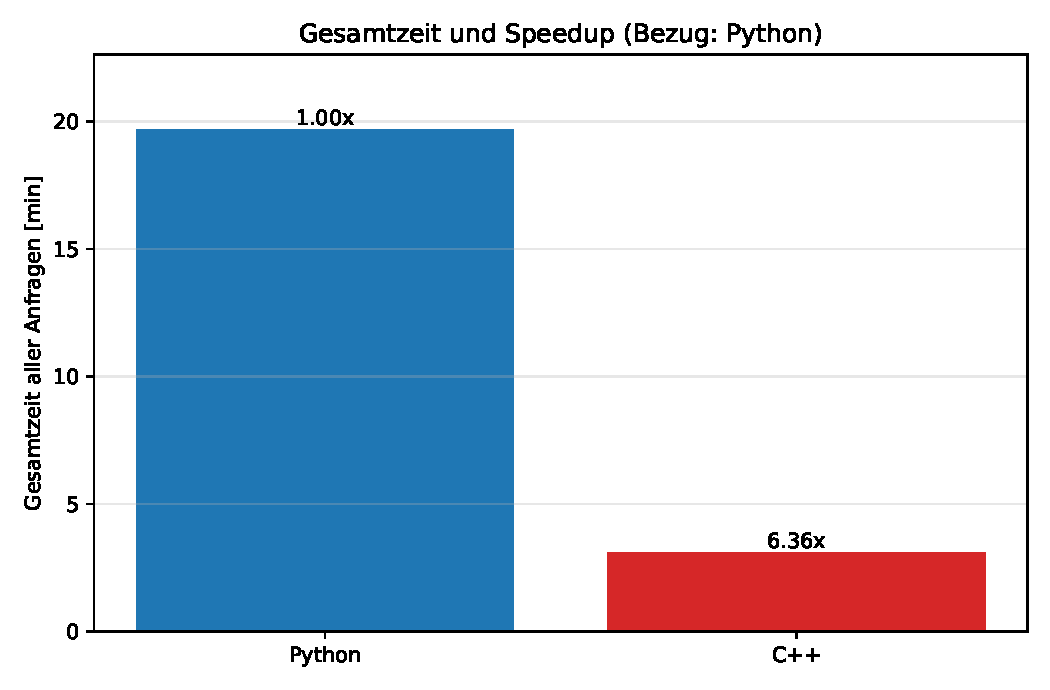
\includegraphics[width=0.75\textwidth]{../src/results/plot6_backends_gesamtzeit_speedup.pdf}
	\caption{Die Gesamtlaufzeit der sechs Suchen sinkt mit der C++-Library gegenüber Python auf rund ein Sechstel.}
	\label{fig:backend_gesamtzeit}
\end{figure}

Abbildung~\ref{fig:backend_gesamtzeit} stellt die aufsummierte Suchzeit in Minuten dar; die Beschriftungen über den Balken geben den Speedup relativ zur Python-Referenz an. Die Differenz ist groß genug, dass sie nicht durch die Wahl einer einzelnen Aggregationskennzahl erklärt wird: Verglichen werden die Summe derselben sechs Antwortzeiten, dieselben Kandidaten und dieselbe Worker-Zahl. Die Grafik belegt den Anwendungseffekt dieser konkreten Library-Integration auf dieser Hardware, nicht eine universelle Beschleunigung für alle Datenbanken oder Query-Arten.

\begin{figure}[!h]
	\centering
	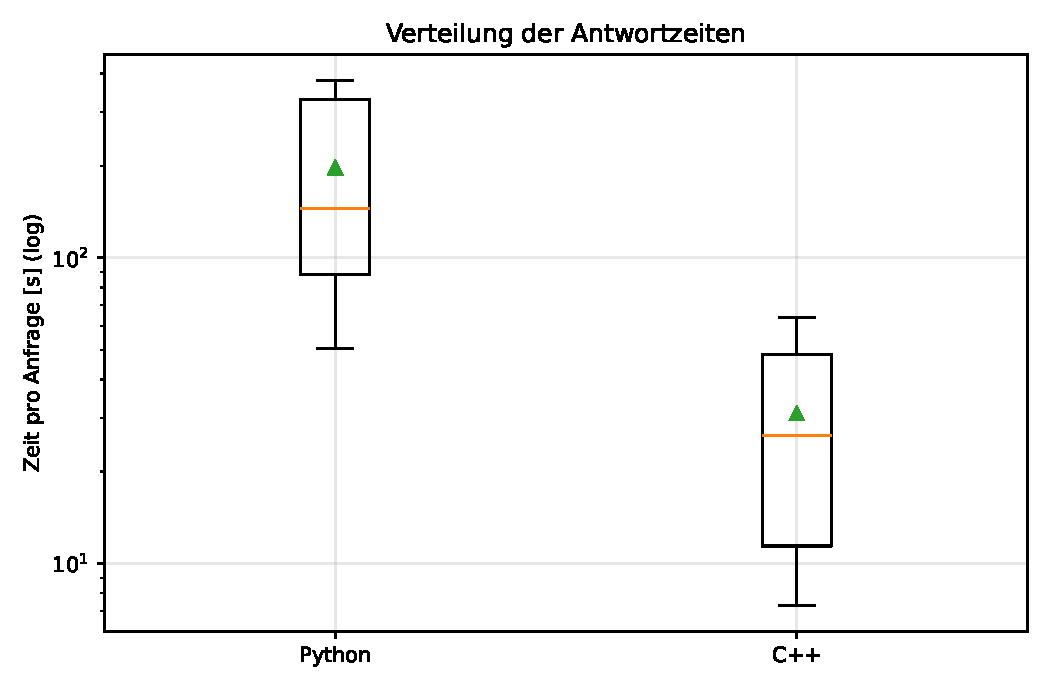
\includegraphics[width=0.75\textwidth]{../src/results/plot7_backends_verteilung_antwortzeiten.pdf}
	\caption{Die Verteilung der sechs Antwortzeiten zeigt für beide Backends eine deutliche Verkürzung bei C++.}
	\label{fig:backend_verteilung}
\end{figure}

Abbildung~\ref{fig:backend_verteilung} verwendet eine logarithmische Zeitachse und zeigt Median, Quartile, Spannweite und Mittelwert der Antwortzeiten. Die beiden Verteilungen liegen klar getrennt: Die mittlere Antwortzeit sinkt von $196{,}7$ auf $30{,}9$ Sekunden, der Median von $145{,}3$ auf $26{,}2$ Sekunden. Die logarithmische Darstellung macht sowohl die Beschleunigung als auch die Unterschiede zwischen kleinen und großen Suchräumen lesbar; die sechs Beobachtungen pro Backend erlauben allerdings keine robuste Aussage über die Verteilung zukünftiger Anfragen.

\subsection{Phasenanalyse und Skalierung mit der Kandidatenzahl}
\label{sec:backend_phasen}

\begin{figure}[!h]
	\centering
	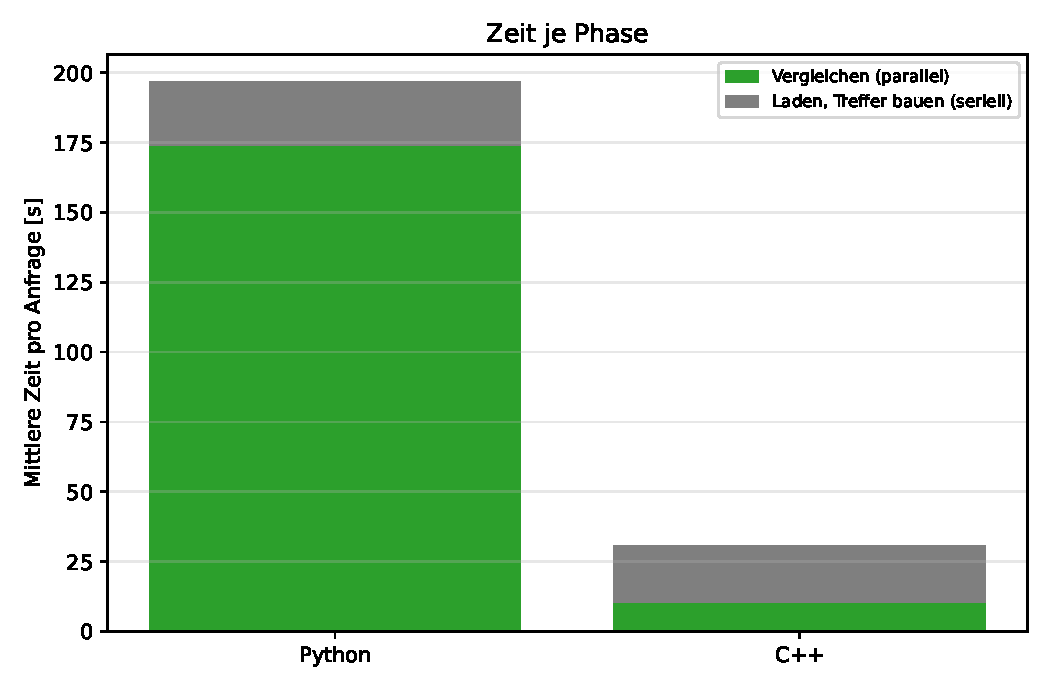
\includegraphics[width=0.75\textwidth]{../src/results/plot8_backends_phasen.pdf}
	\caption{Die Phasenmessung zeigt, wie sich Vergleichszeit und übrige Suchzeit zwischen den Backends verschieben.}
	\label{fig:backend_phasen}
\end{figure}

Abbildung~\ref{fig:backend_phasen} stellt die mittlere Antwortzeit je Anfrage als gestapelte Vergleichsphase und Restzeit dar. Die Python-Vergleichsphase beansprucht aggregiert $88{,}4\,\%$ der Gesamtlaufzeit; bei C++ sind es nur $33{,}3\,\%$. Entsprechend sinkt die Vergleichszeit über die sechs Anfragen von insgesamt rund $1.043$ Sekunden auf rund $61{,}9$ Sekunden, während die gemessene Restzeit von etwa $137$ auf $123{,}7$ Sekunden zurückgeht. Der Rest umfasst Laden, Datenübertragung beziehungsweise Aufgabenverteilung und Ergebnisaufbau und ist nicht mit einer reinen Datenbankzeit gleichzusetzen. Da der Rechenkern nun erheblich schneller ist, wird dieser Anteil relativ dominant: Beschleunigungen weiterer Vergleichsoperationen allein haben abnehmenden Einfluss auf die gesamte Antwortzeit. Strömendes Laden, effizientere Aufgabenübergabe und Phaseninstrumentierung werden dadurch als nächste Optimierungsziele relevanter.

\begin{figure}[!h]
	\centering
	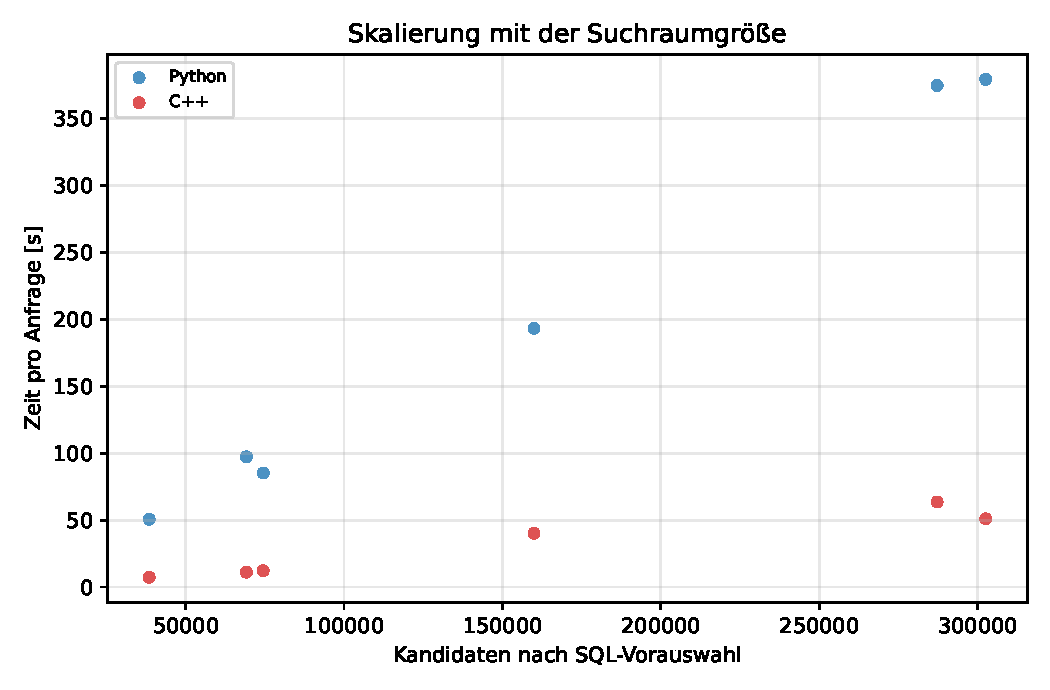
\includegraphics[width=0.75\textwidth]{../src/results/plot9_backends_skalierung_suchraum.pdf}
	\caption{Die Antwortzeit nimmt für beide Backends mit der nach der SQL-Vorauswahl verbleibenden Kandidatenzahl zu.}
	\label{fig:backend_skalierung}
\end{figure}

Abbildung~\ref{fig:backend_skalierung} ordnet jede Anfrage nach der Zahl ihrer Kandidaten und zeigt für Python wie C++ einen klaren Anstieg der Antwortzeit mit wachsendem Suchraum. Die Punkte bilden keine streng proportionale Linie: Queries unterscheiden sich nicht nur in ihrer Kandidatenzahl, sondern auch in Knotenzahl und Struktur, und außerhalb der Vergleichsphase fallen weitere Kosten an. Insgesamt verarbeitet Python rund $790$ Kandidaten pro Sekunde, während die Library rund $5.020$ Kandidaten pro Sekunde erreicht; der aggregierte Aufwand sinkt von $1{,}267$ auf $0{,}199$ Millisekunden je Kandidat. Diese Quotienten beschreiben die sechs vollständigen Suchläufe einschließlich ihrer nichtvergleichenden Anteile und sind deshalb keine isolierten Kosten des Algorithmuskerns.

\begin{figure}[!h]
	\centering
	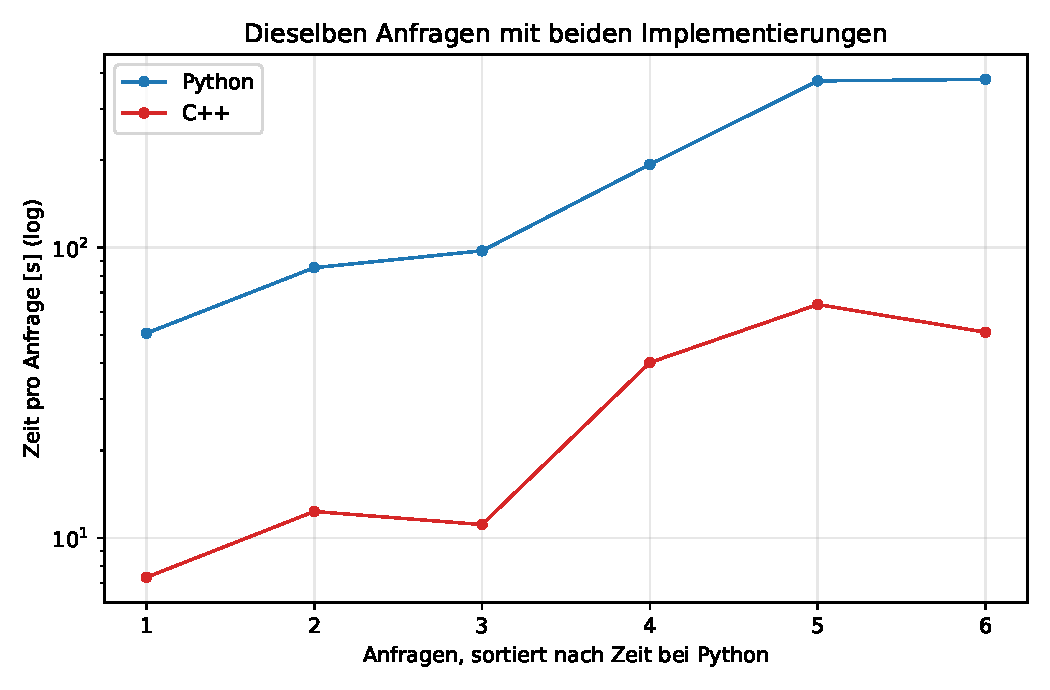
\includegraphics[width=0.75\textwidth]{../src/results/plot10_backends_gleiche_anfragen.pdf}
	\caption{Für jede einzelne Query liegt die Antwortzeit der C++-Library unter derjenigen der Python-Implementierung.}
	\label{fig:backend_queries}
\end{figure}

Abbildung~\ref{fig:backend_queries} zeigt gepaart dieselben sechs Queries, nach der Python-Antwortzeit sortiert und auf logarithmischer Skala. Beide Kurven folgen derselben Reihenfolge: Die aufwendigen Queries bleiben auch mit C++ aufwendiger als die kleineren, jedoch liegt jeder C++-Messpunkt deutlich unter seinem Python-Pendant. Dies schließt aus, dass der aggregierte Vorteil allein aus einer anderen Reihenfolge, einem anderen Query-Sample oder weniger Kandidaten im C++-Lauf entsteht.

\subsection{Mikrobenchmark, funktionale Kontrolle und Diskussion}
\label{sec:backend_diskussion}

Der Mikrobenchmark isoliert die direkten Vergleichsaufrufe auf $200$ identischen Zufallspaaren. Tabelle~\ref{tab:backend_calibration} enthält Mittelwert, Median und Maximum. Der C++-Library-Aufruf benötigt im Mittel $0{,}074$ Millisekunden je Paar, der direkte Python-Aufruf $2{,}694$ Millisekunden. Das Verhältnis der Mittelwerte entspricht einer Beschleunigung von ungefähr $36{,}5\times$; anhand der Mediane ergibt sich etwa $40{,}8\times$. Die Maximalwerte betragen $0{,}331$ beziehungsweise $3{,}703$ Millisekunden. Damit bestätigt H1 für diesen Benchmark deutlich einen schnelleren direkten C++-Aufruf.

Der triviale $1\times1$-Library-Aufruf benötigt im Mittel $0{,}018$ Millisekunden und im Median $0{,}018$ Millisekunden. Das entspricht etwa einem Viertel der mittleren gemessenen C++-Zeit für die größeren Vergleichspaare und zeigt, dass die Funktionsübergabe samt Marshalling nicht null ist, aber weit unter der gemessenen Python-Aufrufzeit liegt. Anders als eine Differenz aus CLI-Messungen ist dieser Wert keine Prozessstartzeit: Er ist ein direkter Aufruf durch die Wrapper-Schnittstelle. Der triviale Aufruf enthält außerdem andere Matrixgrößen als die eigentlichen Paare; er dient daher nur als Größenordnung für die Mindestkosten und nicht als exakt abziehbarer Anteil.

\paragraph{H1 und H2: Beschleunigung des Einzelvergleichs und der Suche.} Der Mikrobenchmark belegt den Geschwindigkeitsvorteil des direkten C++-Aufrufpfads in der Stichprobe. Auch die Ende-zu-Ende-Suche ist mit der Library deutlich schneller: Die Gesamtzeit reduziert sich von $1.180{,}28$ auf $185{,}62$ Sekunden. Der Such-Speedup von $6{,}36\times$ fällt kleiner aus als die etwa $36{,}5\times$ des Mikrobenchmarks, weil die vollständige Anfrage Datenbankzugriff, Prozesskommunikation und Ergebnisaufbau einschließt und weil die Vergleichsphase nach ihrer Beschleunigung nur noch rund ein Drittel der C++-Gesamtzeit ausmacht. Die beiden Speedup-Werte beschreiben damit unterschiedliche Ebenen und widersprechen einander nicht.

\paragraph{H3: funktionale Übereinstimmung.} Für jede Query stimmen die mit Python und C++ gefundenen Netzwerk-IDs überein. Beide Backends liefern je Query einen Treffer, zusammen also sechs Treffer in den sechs jeweiligen Suchläufen. In beiden Reihen beträgt die Fehlerzahl null. Zusätzlich bestätigt die Laufzeitkontrolle, dass die angeforderte Library tatsächlich in den C++-Workern aktiv war. Das ist eine positive differenzielle Prüfung der konkreten sechs Suchläufe, aber noch kein formaler Korrektheitsbeweis für alle Eingaben oder für alle Randfälle des Algorithmus.

\paragraph{H4: Kosten und Grenze der Anbindung.} Der Library-Aufruf verursacht messbare Übergabekosten, doch die direkte Mikrobenchmark-Zeit bleibt deutlich unter der Python-Vergleichszeit. Damit zeigen die neuen Resultate den praktisch relevanten Unterschied zum früheren CLI-Pfad: Dessen Prozess-pro-Vergleich- und JSON-Aufwand hatte einen trivialen Aufruf von rund $10$ Millisekunden ergeben; dieser Wert gehört ausdrücklich nicht zur hier untersuchten Library. Die Funktionseinbindung vermeidet diesen Prozessstart. Sie beseitigt aber weder alle Python/C++-Übergabekosten noch die nichtvergleichenden Phasen der Suchpipeline.

\subsection{Grenzen der Messreihe}
\label{sec:backend_grenzen}

Die Ergebnisse sind positiv, müssen aber innerhalb des Versuchsaufbaus interpretiert werden:

\begin{itemize}
	\item \textbf{Sechs Queries und jeweils ein Suchlauf.} Der Speedup beruht auf sechs mit Seed $42$ reproduzierbar ausgewählten Datenbankanfragen und einer Messung je Backend. Es gibt keine Wiederholungen je Query, Konfidenzintervalle oder Signifikanztests; Cache-, System- und Datenbankzustände können einzelne Zeiten beeinflussen.
	\item \textbf{Synthetische Datenbank und begrenzte Querygrößen.} Die Suchreihe stammt aus der synthetischen Gen-DB-Datenbank; die sechs Queries besitzen $15$ bis $20$ Knoten. Auf realen biologischen Netzwerken, anderen Dichten und größeren Matrizen kann sich das Verhältnis ändern.
	\item \textbf{Spezifische Hardware und Implementierung.} Gemessen wurde unter Windows 11 mit Python $3.14.8$, vier logischen Prozessoren und zwei Workern. Compileroptionen, Prozessorarchitektur, Betriebssystem, Datenbanklast und Wrapper beeinflussen die Laufzeiten.
	\item \textbf{Mikrobenchmark ist kein vollständiger Algorithmusvergleich.} Die $200$ Zufallspaare decken Matrizen mit $15$ bis $20$ Knoten und Kantendichte um $0{,}3$ ab. Sie belegen den Vorteil unter dieser Verteilung, aber nicht für alle Graphklassen. Der Vergleich schließt zudem die konkrete Python-zu-C++-Übergabe ein.
	\item \textbf{Phasenrest ist zusammengesetzt.} Die Differenz zwischen Suchzeit und Vergleichszeit verbindet mehrere Vorgänge und darf weder als reine Datenbanklaufzeit noch als reine Parallelisierungskosten ausgelegt werden. Eine feinere Instrumentierung wäre nötig, um die verbliebenen rund zwei Drittel der C++-Zeit kausal aufzuteilen.
	\item \textbf{Trefferabgleich ist kein universeller Nachweis.} Identische Treffer-IDs und null Fehler in dieser Stichprobe erhöhen das Vertrauen in die Integration, ersetzen aber keine gemeinsamen Konformitäts- und Eigenschaftstests für alle Eingabekombinationen.
\end{itemize}

\subsection{Fazit}
\label{sec:backend_zwischenfazit}

Der Wechsel von Python zur C++-Library beschleunigt in der gemessenen Konfiguration sowohl den direkten Vergleich als auch die vollständige Suche. Bei denselben sechs Anfragen und $931.899$ Kandidaten sinkt die Gesamtzeit um den Faktor $6{,}36$; in allen sechs Fällen stimmen die Treffer-IDs überein, und es gibt keine fehlgeschlagenen Vergleiche. Der Mikrobenchmark misst einen noch größeren Vorteil für direkte Aufrufe, während die Phasenanalyse zeigt, dass Laden, Übergabe und Ergebnisaufbau den Ende-zu-Ende-Speedup begrenzen. Die Messergebnisse stützen damit die Library-Integration als sinnvollen Beschleunigungsweg für diesen Anwendungsfall. Sie sind wegen Stichprobengröße, synthetischer Daten und einzelner Hardwarekonfiguration eine belastbare Tendenz, aber keine universelle Leistungsgarantie.

Dass der Bytecode für die C++-Library größer ist, ist deshalb so, weil dadurch im Arbeitsspeicher ein größerer Bereich reserviert wird, der viel effizienter von der Architektur zur Ausführung prozessiert werden kann. Wenn der reservierte Bereich dagegen kleiner ist, wie für die Python Implementierung des Subgraph Algorithmus, ist der reservierte Speicherbereich kleiner.

Der Strom im reservierten Bereich im Arbeitsspeicher für den Algorithmus liegt parallel an. Ist dieser Bereich kleiner, kann die effiziente Architektur mit Adressbus, Datenbus, Steuerbus und Controller diesen Bereich nicht so schnell ausführen und bearbeiten wie für reservierte Bereiche die größer sind.

Es ist so, dass diese hochentwickelte und für Geschwindigkeit extrem ausgelegte Hardware-Architektur des Prozessors gerade darauf wartet, durch die parallele Bestromung der reservierten Bereiche im Arbeitsspeicher möglichst viele Instruktionen dadurch gleichzeitig prozessieren zu können. Etwas enttäuscht ist sie dann doch, wenn der reservierte Bereich kleiner ist und sie gerade für ihre eigentliche Bestimmung so  nicht so sehr zum Ziel kommen kann, was die Ausführung des Subgraph Algorithmus verzögert.

\subsection{Fremde Beschreibungen}
\label{sec:fremde_beschreibungen}
Die Anreicherung mit einem Fremdmodul in einer anderen Beschreibung erscheint mir sehr unpassend und beschreibungstechnisch nicht durchgängig. Eine lose Kopplung dagegen, angenommen durch eine C++-CLI oder C++-Library, erlaubt eine klarere Trennung, bei der alle beteiligten Mitgestalter dieses Softwaresystems mit einem klaren Trennungsbewusstsein dieses System mitgestalten. Ein System, das aus Bereichen oder Teilen besteht, die durch unterschiedliche Beschreibungen entwickelt sind oder arbeiten, schafft Mitgestaltern dieses Systems ein in der Regel eher unruhigeres Trennungsbewusstsein in der Analyse, Weiterentwicklung und Wiederverwendung.
Dieses unruhigere Trennungsbewusstsein kann sich in der Praxis in einer unklaren Verantwortlichkeit und Kostenverteilung an der Grenze zwischen den beiden Beschreibungen äußern. Die Messungen dieses Kapitels dagegen zeigen für Gen-DB zugleich einen deutlichen Laufzeitvorteil der Library. Die weitergehende Position dieser Arbeit lautet, dass klar benannte Grenzen Analyse, Weiterentwicklung und Wiederverwendung unterstützen und dadurch ein gemeinsames Trennungsbewusstsein fördern. Diese Aussage ist eine begründete Gestaltungsposition; die Laufzeitdaten allein messen sie nicht.

Die Einbindung eines Fremdmoduls aus einer anderen Beschreibung wirft eine Gestaltungsfrage auf: Wie bleiben Verantwortlichkeiten und Kosten an der Grenze für alle Mitgestaltenden erkennbar? Eine lose Kopplung über eine C++-Library statt über einen separaten C++-CLI-Prozess hält die technische Schnittstelle schmaler und ermöglicht es, den C++-Kern innerhalb des Python-Workers aufzurufen. Die Messungen dieses Kapitels zeigen für Gen-DB zugleich einen deutlichen Laufzeitvorteil der Library. Die weitergehende Position dieser Arbeit lautet, dass klar benannte Grenzen Analyse, Weiterentwicklung und Wiederverwendung unterstützen und dadurch ein gemeinsames Trennungsbewusstsein fördern. Diese Aussage ist eine begründete Gestaltungsposition; die Laufzeitdaten allein messen sie nicht.

Dieser Abschnitt führt die Aussage weiter aus. Er klärt zunächst, was hier unter einer \emph{Beschreibung} verstanden wird, wendet die Aussage dann auf die Messungen dieses Kapitels an und überträgt sie anschließend auf die übrigen Teile der Arbeit. Abschließend werden Gegenargumente und die Grenzen der Position benannt. Wichtig ist die Reihenfolge der Argumente: Die Position beruht in erster Linie auf einer Überlegung zur Gestaltung des Systems. Die Messwerte aus diesem Kapitel illustrieren sie, sie beweisen sie nicht.

\subsubsection{Was hier unter einer Beschreibung verstanden wird}
\label{sec:fremde_begriff}

Eine \emph{Beschreibung} bezeichnet im Folgenden die Gesamtheit der Vereinbarungen, in denen ein Teil eines Systems formuliert ist: seine Sprache, seine Datentypen, sein Fehlermodell, die Lebensdauer seiner Zustände und die Art, wie er aufgerufen, getestet und ausgeliefert wird. Zwei Teile liegen in derselben Beschreibung, wenn sie diese Vereinbarungen teilen. Dann kann ein Mitgestalter, der den einen Teil versteht, den anderen mit denselben Begriffen lesen. Ein \emph{Fremdmodul} ist ein Teil, der in einer anderen Beschreibung arbeitet und dennoch Teil desselben Systems sein soll.

Gen-DB besteht in der Beschreibung des Backends aus Python-Code. Matrizen liegen dort als \texttt{numpy}-Arrays vor, Fehler werden über Python-Ausnahmen signalisiert, und der Subgraph Algorithmus wird als Funktion oder Objekt aufgerufen. Die frühere C++-CLI arbeitete dagegen in einer anderen Beschreibung: Matrizen wurden zu JSON-Text, Fehler zu Exit-Codes und Ausgaben auf \texttt{stderr}, und ein Zustand überlebte keinen Aufruf. Die nun eingesetzte Library behält den nativen C++-Kern bei, stellt dem Backend aber eine direkte Funktionsschnittstelle im Worker-Prozess bereit. Sie benötigt weiterhin eine Sprachgrenze und eine passende Fehler- und Datentypabbildung, vermeidet jedoch das pro Vergleich wiederholte Textprotokoll und den zusätzlichen Prozesslebenszyklus.

Die C++-Library ist ebenfalls in C++ geschrieben, ihre Schnittstelle kann jedoch in der Beschreibung des Aufrufers erscheinen, etwa als importierbare Funktion, die Arrays entgegennimmt und Werte oder Ausnahmen zurückgibt. Der Unterschied liegt also nicht in der Programmiersprache des Algorithmuskerns, sondern darin, \emph{wo die Grenze zwischen beiden Beschreibungen verläuft}. Bei der Library verläuft sie an einer schmalen, typisierten Funktionsschnittstelle. Bei der CLI verläuft sie am Betriebssystem, also an Prozessgrenze, Textformat und Dateideskriptoren.

\subsubsection{Anwendung auf die Messungen dieses Kapitels}
\label{sec:fremde_messung}

Die Untersuchung unterscheidet zwischen der früheren CLI-Anbindung und der nun gemessenen Library-Anbindung. Die CLI legte eine breite Grenze aus Prozessstart, Textformat und Fehlerauswertung offen; die Library verläuft innerhalb des Worker-Prozesses über einen Funktionsaufruf. Der Mikrobenchmark und die Ende-zu-Ende-Messung quantifizieren den Laufzeitunterschied dieser konkreten Varianten.

\paragraph{Der Messaufbau überwacht die aktive Implementierung.} Die Versuchsanordnung prüft die tatsächlich in den Worker-Prozessen aktive Implementierung, zählt fehlgeschlagene Einzelvergleiche und vergleicht die Treffer-IDs beider Backends (Abschnitt~\ref{sec:backend_versuchsaufbau}). Diese Kontrollen sind nötig, um den konkreten Lauf korrekt zuzuordnen und Backend-Konformität empirisch zu prüfen. Sie zeigen zugleich, dass sprachübergreifende Integration Tests an der Grenze benötigt; der abgeschlossene Lauf bestätigt für die sechs Queries gleiche Treffer-IDs und null Fehler.

\paragraph{Fachliche Regeln müssen an der Schnittstelle eindeutig sein.} Der C++-Kern liefert Ergebniswerte, die auf die von Gen-DB verwendeten Zustände abgebildet werden; bei identischen Graphen muss außerdem dieselbe Auswahlregel wie im Python-Backend gelten. Solche Regeln dürfen bei austauschbaren Backends nicht implizit auseinanderlaufen. Die Library beseitigt nicht automatisch diese semantische Verantwortung, ermöglicht aber eine gemeinsame Funktionsschnittstelle und direkte Konformitätstests ohne JSON-Protokoll. Eine ausdrücklich dokumentierte Spezifikation bleibt daher erforderlich.

\paragraph{Die Library-Schnittstelle ist messbar, aber klein gegenüber dem CLI-Prozesspfad.} Der direkte Mikrobenchmark (Tabelle~\ref{tab:backend_calibration}) misst für C++ im Mittel $0{,}074$ Millisekunden je Vergleich und $0{,}018$ Millisekunden für einen trivialen $1\times1$-Aufruf. Letzterer ist eine Größenordnung für Funktionsübergabe und Marshalling; er entspricht ungefähr einem Viertel der mittleren Zeit des regulären Library-Aufrufs. Dem steht der frühere CLI-Mikrobenchmark mit $10{,}081$ Millisekunden für den trivialen Prozessaufruf gegenüber. Die Werte stammen aus verschiedenen Messläufen und Aufrufpfaden; sie dürfen nicht als exakt kontrollierter A/B-Vergleich subtrahiert werden. Zusammen mit dem gemessenen Ende-zu-Ende-Speedup von $6{,}36\times$ zeigen sie jedoch, dass die Library die Kostenstruktur der CLI vermeidet und den nativen Rechenkern praktisch nutzbar macht.

\paragraph{Der Prozess-Pool wird mit der Library wiederverwendet.} Gen-DB betreibt einen langlebigen \texttt{ProcessPoolExecutor}, dessen Worker Kandidaten blockweise mit je $256$ Vergleichen bearbeiten. Die Library wird einmal je Worker geladen und für die Vergleiche innerhalb dieses Prozesses wiederverwendet. Die frühere CLI öffnete zusätzlich einen Prozess pro Vergleich; dieser zweite Prozess-Lebenszyklus entfällt im nun gemessenen Pfad. Das passt zum Modell der Anwendung und vermeidet wiederholte Betriebssystem- und JSON-Kosten.

\subsubsection{Anwendung auf die gesamte Arbeit}
\label{sec:fremde_gesamt}

Die Position betrifft nicht nur dieses Kapitel. Sie knüpft an den Gedanken an, den die Schlussbemerkung als zentral bezeichnet, nämlich die Trennung zweier Aufgaben: eine günstige Vorauswahl in der Datenbank und der Subgraph Algorithmus als Entscheidung über jeden verbliebenen Kandidaten. Diese Trennung funktioniert, weil sie klar ist. Eine Anbindung, die sie an anderer Stelle durch eine unscharfe Grenze unterläuft, widerspricht dem Prinzip der Gesamtarbeit.

\paragraph{Systemarchitektur (Abschnitt~\ref{sec:architektur}).} Die drei Schichten Frontend, Backend und Datenbank sind jeweils durch eine benannte Schnittstelle getrennt: REST-Aufrufe zwischen Frontend und Backend, SQL zwischen Backend und Datenbank. Der Algorithmus wird vom Modul \texttt{crud.py} über seine Backend-API aufgerufen. Die C++-Library wird innerhalb dieses Backend-Bausteins geladen und fügt keine weitere Prozessgrenze in die Suchpipeline ein.

\paragraph{Formale Analyse (Abschnitt~\ref{sec:pipeline}).} Satz~\ref{satz:pipeline} modelliert die Suchzeit als Summe aus dem Pre-Filter und $C$ Vergleichen mit je $O(n^3)$ Aufwand. Das Modell trägt, solange die Kosten eines Vergleichs dem Algorithmus zugerechnet werden können. Eine Prozess-pro-Vergleich-Anbindung fügt jedem Vergleich einen Term hinzu, den das Modell nicht enthält.

\begin{bemerkung}[Erweitertes Kostenmodell]
\label{bem:schnittstellenkosten}
Bezeichne $\delta$ die Schnittstellenkosten je Vergleich. Bei der CLI umfassen sie Prozessstart, JSON-Serialisierung und Antwortauswertung; bei der Library die Übergabe der Arrays und den Funktionsaufruf. Dann lautet eine erweiterte Form des Modells aus Satz~\ref{satz:pipeline}
\[
	T'_{\text{Suche}}(N,C,n) = O(\log N + C) + O\bigl(C\cdot(n^3+\delta)\bigr).
\]
Der direkte Mikrobenchmark misst für die Library $0{,}018$ ms für einen trivialen Funktionsaufruf und $0{,}074$ ms im Mittel für ein Zufallspaar. Der frühere CLI-Mikrobenchmark maß rund $10$ ms für den trivialen Prozessaufruf. Diese konkreten Zeiten hängen von Hardware, Datenformat und Umgebung ab; sie zeigen jedoch, dass $\delta$ je nach Anbindung einen erheblichen Unterschied im konstanten Faktor erzeugt. Aus den Werten lässt sich kein allgemeiner Vergleich von $\delta$ mit der abstrakten Zahl $n^3$ ableiten.
\end{bemerkung}

Das erweiterte Modell erhält die asymptotische Aussage, dass die Suchzeit linear mit $C$ wächst. Es macht aber sichtbar, dass die Wahl der Anbindung den konstanten Faktor bestimmt. Ein Modell mit einem Term, den die Beschreibung der Arbeit nicht benennt, wäre ein Beispiel für das beschriebene Problem im Kleinen.

\paragraph{Empirische Evaluation und VF2-Vergleich (Abschnitte~\ref{sec:evaluation} und~\ref{sec:vergleich}).} Der Vergleich mit VF2 ist aussagekräftig, weil beide Verfahren in derselben Beschreibung laufen: Beide werden in Python aufgerufen, auf identischen Eingaben und mit derselben Zeitmessung. Die Library-Messung vergleicht zwei unterschiedliche Implementierungssprachen, aber beide Aufrufe erfolgen innerhalb der Suchworker und auf denselben Daten. Sie misst damit den realen Einfluss der Backend-Wahl auf Gen-DB und nicht ausschließlich den algorithmischen Aufwand. Der frühere CLI-Pfad hatte zusätzlich Prozessstart und JSON-Transport in die Messung eingebracht.

\paragraph{Parallelisierung (Abschnitt~\ref{sec:parallel}).} Die dort gemessenen Ergebnisse, ein Speedup von $1{,}90$ mit zwei Workern und eine Verschlechterung beim dritten Worker auf einem Rechner mit zwei logischen Prozessoren, beschreiben die Python-Arbeitslast. Der Backend-Versuch setzte zwei Worker ein und zeigte auch bei der Library einen deutlichen Suchgewinn; er untersuchte jedoch nicht systematisch unterschiedliche Worker-Zahlen. Daher bleibt offen, ob die optimale Parallelisierung und der serielle Anteil mit C++ unverändert sind. Die Worker-Zahl sollte weiterhin an verfügbare Prozessoren und die Last des Datenbankservers angepasst werden.

\paragraph{Schluss und Ausblick (Abschnitte~\ref{sec:grenzen} und~\ref{sec:ausblick}).} Die Grenzen der Arbeit nennen eine in reinem Python geschriebene Referenzimplementierung als obere Abschätzung des praktisch Erreichbaren. Der Ausblick führt als Hebel die Vektorisierung mit \texttt{numpy}, die Kompilierung mit \texttt{numba} und die C++-Erweiterung auf (Abschnitt~\ref{sec:impl_opt}). Alle drei sind Anbindungen, die in der Beschreibung des Aufrufers bleiben. Die hier vertretene Position stützt diese Reihenfolge: Weiterentwicklungen des Vergleichs sollten zuerst dort ansetzen, wo die Grenze schmal bleibt, und die Prozessgrenze nur dort einführen, wo ihr Zweck, etwa Isolation, den Beschreibungsbruch rechtfertigt.

\subsubsection{Kriterien einer losen Kopplung}
\label{sec:fremde_kriterien}

Aus den vorangehenden Überlegungen lassen sich Kriterien ableiten, an denen sich beide Anbindungsformen vergleichen lassen. Die Tabelle fasst Gestaltungseigenschaften zusammen; die Laufzeitangaben werden durch die Mikro- und Suchmessungen aus Abschnitt~\ref{sec:backend_zwischenstand} ergänzt.

\begin{table}[!h]
	\centering
	\small
	\caption{Vergleich der früheren CLI- und der nun umgesetzten Library-Anbindung nach Gestaltungskriterien.}
	\label{tab:fremde_kriterien}
	\begin{tabular}{@{}>{\raggedright\arraybackslash}p{3.0cm}>{\raggedright\arraybackslash}p{5.6cm}>{\raggedright\arraybackslash}p{5.6cm}@{}}
		\toprule
		Kriterium & C++-CLI (Prozess pro Vergleich) & C++-Library (im Worker-Prozess) \\
		\midrule
		Datenaustausch & Matrizen als JSON-Text über \texttt{stdin} und \texttt{stdout} & typisierte Arrays über eine Funktionsschnittstelle \\
		Fehlermodell & Exit-Code, \texttt{stderr}, Timeout (\texttt{CSUBGRAPH\_TIMEOUT}) & Ausnahmen oder Rückgabewerte in der Beschreibung des Aufrufers \\
		Lebensdauer & kein Zustand über einen Vergleich hinaus & Instanz je Worker, wiederverwendbar \\
		Aufrufkosten $\delta$ & Prozessstart je Vergleich, früher etwa $10$ ms je trivialem Aufruf & Funktionsaufruf im Prozess, trivial im Mittel $0{,}018$ ms \\
		Ergebnisregeln & Übersetzung der Werte und Regel für identische Graphen im Backend & Abbildung kann Teil der Schnittstelle sein und liegt dann beim Algorithmus \\
		Testbarkeit & Tests brauchen ein gebautes Executable und einen Prozessstart & Tests rufen die Funktion direkt auf, gleiche Mittel wie beim Python-Algorithmus \\
		Auslieferung & plattformabhängiger Pfad zum Executable (\texttt{subgraph-cli.exe}) über die Konfiguration & Abhängigkeit des Projekts, Binärdatei je Plattform \\
		Isolation & Absturz des Algorithmus betrifft nur den Einzelprozess & Absturz betrifft den Worker-Prozess \\
		Messbarkeit & Schnittstellenkosten verdecken den Rechenkern & Rechenkern lässt sich unter gleichen Bedingungen wie Python messen \\
		\bottomrule
	\end{tabular}
\end{table}

Die Zeile zur Isolation zeigt, dass die Gegenüberstellung nicht einseitig ausfällt. Sie ist die stärkste Gegenposition und wird im nächsten Abschnitt behandelt.

\subsubsection{Gegenargumente und Grenzen der Position}
\label{sec:fremde_gegen}

\paragraph{Isolation und Sprachneutralität.} Eine CLI trennt Prozesse hart. Ein Fehler im nativen Code reißt dann nicht den Worker mit, und ein Timeout kann den Prozess beenden. Außerdem ist eine CLI von jeder Sprache aus aufrufbar. Beide Eigenschaften sind echte Vorteile. Sie sprechen für die CLI als Werkzeug, etwa für Skripte, manuelle Prüfungen oder Experimente. Die hier vertretene Position betrifft die Einbindung in das System. Für diese zählt, ob die Grenze in der gemeinsamen Beschreibung des Systems liegt. Die CLI bleibt als eigenständiges Programm sinnvoll, auch wenn Gen-DB den Algorithmus über die Library aufruft.

\paragraph{Aufwand der Library.} Eine Library braucht eine Anbindung an Python, etwa über einen Erweiterungsmechanismus, und eine Bauumgebung je Plattform. Das ist Aufwand, den die CLI zunächst nicht verlangt. Die Position behauptet nicht, dass dieser Aufwand gering sei. Sie behauptet, dass er einmalig anfällt und die Grenze danach schmal hält, während die Kosten der CLI bei jedem Vergleich und bei jeder Weiterentwicklung wiederkehren.

\paragraph{Die Evidenz ist begrenzt, aber nicht mehr vorläufig.} Die Library wurde im Mikrobenchmark und in einer vollständigen Suchreihe gemessen; beide Messungen zeigen einen deutlichen Zeitgewinn. Die Aussagekraft ist jedoch auf sechs Queries, einen Lauf je Backend und eine Hardwarekonfiguration begrenzt. Die Ergebnisse belegen daher den Vorteil in diesem Versuchsaufbau, nicht für jede Plattform oder Graphenfamilie.

\paragraph{Die Position ist eine Gestaltungsentscheidung.} Begriffe wie Trennungsbewusstsein lassen sich in dieser Arbeit nicht messen. Sie bezeichnen eine Eigenschaft der Zusammenarbeit von Mitgestaltern, die durch Fallbeispiele wie die oben genannten plausibel gemacht, aber nicht durch eine Studie belegt wird. Die Arbeit formuliert sie deshalb als begründete Position und nicht als Ergebnis.

\subsubsection{Folgerungen für Gen-DB}
\label{sec:fremde_folgerungen}

Aus der Position und den Messungen ergeben sich fünf Folgerungen für die weitere Arbeit am System:

\begin{enumerate}
	\item \textbf{Eine Schnittstelle, mehrere Implementierungen.} Python- und C++-Algorithmus sollten hinter derselben Funktionsschnittstelle liegen. Der Aufrufer in Gen-DB wählt die Implementierung über die Konfiguration, und der Rückfall auf Python bleibt erhalten. Er ist dann ein Wechsel hinter einer gemeinsamen Schnittstelle und kein Wechsel der Beschreibung.
	\item \textbf{Fachliche Regeln gehören zum Algorithmus.} Die Abbildung der Ergebniswerte und die Auswahl nach der Kantenzahl bei identischen Graphen sollten in der Schnittstelle des Algorithmus festgelegt sein und nicht im Übersetzungscode der Anwendung. Beide Implementierungen liefern dann per Konstruktion dieselben Werte, und die Kontrolle über die Treffer-IDs wird zu einem Test statt zu einer Laufzeitprüfung.
	\item \textbf{Die Library-Messung verbreitern.} Die erste gepaarte Messreihe liegt vor. Als nächstes sollte sie mit mehr Queries, Wiederholungen, Konfidenzintervallen und weiteren Plattformen wiederholt werden; die Vergleiche sollten dabei nach Suchphasen aufgeschlüsselt werden.
	\item \textbf{Schnittstellenkosten ausweisen.} Künftige Messungen sollten $\delta$ getrennt von der Rechenzeit des Algorithmus berichten, wie es die Bemerkung~\ref{bem:schnittstellenkosten} nahelegt. Dadurch lassen sich Ergebnisse verschiedener Anbindungen vergleichen, ohne Algorithmus und Schnittstelle zu vermischen.
	\item \textbf{Die CLI als Werkzeug behalten.} Die CLI bleibt für Einzelprüfungen, Skripte und Fehlersuche nützlich. Sie sollte jedoch nicht der Pfad sein, über den die produktive Suche einen Vergleich nach dem anderen ausführt.
\end{enumerate}

\subsubsection{Zwischenfazit zur Kopplung}
\label{sec:fremde_fazit}

Die Aussage des Abschnitts lässt sich so zusammenfassen: Ein System bleibt analysierbar, weiterentwickelbar und wiederverwendbar, wenn seine Grenzen schmal und benannt sind und die Zuständigkeiten klar bleiben. Die Messungen zeigen am Beispiel der C++-Anbindung sowohl einen strukturellen als auch einen Laufzeitunterschied: Die CLI verlegt die Grenze an Prozess, JSON-Text und Exit-Code; der frühere triviale Aufruf benötigte rund $10$ ms. Die Library wird dagegen direkt im Worker aufgerufen; ihr trivialer Aufruf lag im Mittel bei $0{,}018$ ms, und die vollständige Suche war $6{,}36$-mal schneller als mit Python. Der Suchlauf bestätigt damit einen konkreten Leistungsvorteil dieser Library-Integration. Die allgemeinere Behauptung, dass dadurch Zusammenarbeit und Wiederverwendung erleichtert werden, bleibt eine begründete Gestaltungsposition. Die Library setzt in der Gesamtarbeit das Prinzip fort, das Architektur, formale Analyse und Messmethodik tragen: Schnittstellen und ihre Kosten sichtbar zu machen, statt sie im Gesamtergebnis zu verbergen.

\section{Experimentelle Untersuchung Multi-Omics-Suche}
\label{sec:multiomics}

Die bisherigen Such- und Backend-Experimente vergleichen jeweils einzelne Netzwerke. Biologische Prozesse lassen sich jedoch häufig erst dann sinnvoll untersuchen, wenn mehrere Datenebenen gemeinsam betrachtet werden: Genom, Transkriptom, Proteom und Metabolom beschreiben unterschiedliche, miteinander in Beziehung stehende Aspekte eines Systems. Dieses Kapitel erweitert deshalb die Suche von einer einzelnen Adjazenzmatrix auf ein geordnetes Bündel mehrerer Netzwerkschichten. Im Mittelpunkt stehen nicht nur Laufzeit und Implementierung, sondern auch die Frage, ob die beiden Backends für verschiedene Arten der Schichtkopplung dieselben Entscheidungen treffen.

Die Untersuchung wird durch \texttt{src/experiment\_search\_multiomics.py} gesteuert. Der Lauf wurde am 8. Oktober 2026 nach Abschluss der Such-, Worker- und Chunk-Größen-Experimente während der Datenbankgrößenreihe abgebrochen. Die JSON-Datei wird nach jeder Messung aktualisiert und enthält deshalb vollständige Resultate für diese drei Phasen, aber nur einen Teil der Datenbankgrößenmessungen. Die folgenden Aussagen trennen diese abgeschlossenen Reihen von der abgebrochenen Phase. Die maschinenlesbaren Einzelergebnisse stehen in \texttt{src/results/search\_multiomics\_20261008\_115430.json}; das Textprotokoll \texttt{src/results/search\_multiomics\_20261008\_115430.txt} dokumentiert den Ablauf und den Abbruchstand.

\subsection{Mehrschichtige Netzwerke und Suchrelationen}
\label{sec:multiomics_relation}

Ein Multi-Omics-Netzwerk wird als geordnetes Tupel
\[
\mathcal{M}=(A_1,A_2,\ldots,A_L), \qquad A_\ell\in\{0,1\}^{n\times n},
\]
modelliert. Jede Matrix $A_\ell$ repräsentiert eine Omics-Schicht, beispielsweise ein Genom- oder Proteomnetzwerk. In diesem Experiment haben alle Schichten eines Tupels dieselbe Knotenzahl $n$; die Schichtnamen bleiben jedoch unterscheidbar. Verglichen werden Query-Tupel und Kandidaten-Tupel mit möglicherweise verschiedener Knotenzahl und Schichtzahl.

Der Vergleich baut auf den Zeilenkomponenten der Matrizen auf, also den aus den Spalten abgeleiteten Bitmustern des in Abschnitt~\ref{sec:grundlagen} beschriebenen Subgraph Algorithmus. Eine einzelne Schichtrelation sucht ein benachbartes Paar solcher Komponenten in zyklischer Ordnung. Für mehrere Schichten unterscheidet die Implementierung zwei Kopplungsmodi:

\begin{itemize}
\item \textbf{Kohärent:} Ein passendes Komponentenpaar der Query muss in allen betrachteten Schichten an derselben Kandidatenposition auftreten. Die Schichten teilen damit eine gemeinsame strukturelle Einbettung.
\item \textbf{Unabhängig:} Jede Schicht darf ihr passendes Komponentenpaar an einer eigenen Kandidatenposition finden. Die Trefferpositionen müssen zwischen den Schichten nicht übereinstimmen.
\end{itemize}

Die kohärente Bedingung ist die strengere Kopplung: Ein kohärenter Treffer erfüllt auch die unabhängige Bedingung. Die Modi beantworten somit unterschiedliche fachliche Fragen. Kohärent sucht nach einem über mehrere Ebenen hinweg an derselben Stelle erhaltenen Muster; unabhängig fragt, ob das Muster in jeder Ebene vorkommt, auch wenn die Positionen voneinander abweichen. Das Experiment prüft diese Unterscheidung anhand gezielt konstruierter Beispiele und darf nicht mit einer validierten biologischen Kausalbeziehung zwischen den Schichten gleichgesetzt werden.

\subsection{Versuchsaufbau und Datengenerierung}
\label{sec:multiomics_setup}

Der Lauf verwendet den Seed $42$ und ergänzt die bestehende Datenbank um $20.000$ reproduzierbar erzeugte Zufallsnetzwerke des Typs \texttt{multi\_omics\_experiment}. Hinzu kommen Netzwerke, die zu eingebetteten Queries eine bekannte Lösung liefern; zum gespeicherten Zwischenstand enthielt die Datenbank insgesamt $20.175$ Multi-Omics-Netzwerke. Die Zufallsnetzwerke haben $4$ bis $40$ Knoten und $2$ bis $5$ Schichten. Für die Schichten werden sechs Namen aus Genom, Transkriptom, Proteom, Metabolom, Epigenom und Lipidom verwendet. Die Schichten werden als gerichtete Zufallsmatrizen ohne Selbstkanten mit je Omics-Typ festgelegter Kantenwahrscheinlichkeit erzeugt.

Das Query-Gitter umfasst sieben Knotenzahlen ($4,6,8,12,16,24,32$), vier Schichtzahlen ($1$ bis $4$) und zwei Query-Arten: eine Zufallsanfrage ohne absichtlich eingefügte Lösung sowie eine Anfrage, zu der Lösungen konstruiert werden. Damit entstehen $56$ Query-Konfigurationen. Zu den eingebetteten Anfragen werden eine identische Kopie, kohärent eingebettete und unabhängig eingebettete Kandidaten erzeugt. Für die Einbettung werden zwei benachbarte Query-Spalten in die Kandidatenmatrix kopiert; Zeilen außerhalb der Query-Knotenzahl bleiben dabei null. Bei kohärenten Beispielen verwenden alle Schichten dasselbe benachbarte Paar und dieselbe Position, bei unabhängigen Beispielen kann die Position je Schicht variieren. Die so erzeugten Kandidaten stellen eine Ground Truth bereit, unabhängig davon, ob Python und C++ dieselbe Antwort liefern.

\begin{table}[!h]
\centering
\small
\caption{Konfiguration des Multi-Omics-Experiments gemäß gespeicherten Laufmetadaten.}
\label{tab:multiomics_setup}
\begin{tabular}{@{}>{\raggedright\arraybackslash}p{5.2cm}>{\raggedright\arraybackslash}p{8.2cm}@{}}
\toprule
Parameter & Wert \\
\midrule
Zufallsnetzwerke & $20.000$, $4$--$40$ Knoten und $2$--$5$ Schichten \\
Omics-Schichten & Genom, Transkriptom, Proteom, Metabolom, Epigenom, Lipidom \\
Query-Knotenzahlen & $4,6,8,12,16,24,32$ \\
Query-Schichtzahlen & $1,2,3,4$ \\
Query-Arten und Modi & Zufall/eingebettet; kohärent/unabhängig \\
Suchmessungen geplant & $56$ Queries $\times 2$ Modi $\times 2$ Backends $\times 3$ Wiederholungen $=672$ \\
Mikrobenchmark & $6$ Schichtzahlen $\times 6$ Knotenzahlen $\times 2$ Paartypen; je $100$ Vergleiche \\
Korrektheitsprüfung & $5.000$ Paare; beide Modi, bekannte Konstruktionen und Zufallspaare \\
Worker-Skalierung & $1,2,3,4$ Worker; Standardausführung mit $2$ Workern \\
Chunk-Größen & $1,8,32,128,256,1024,4096$ \\
Datenbankgrößen & $2.000,5.000,10.000,20.000$ Zufallsnetzwerke \\
Wiederholungen & $3$ pro Suchkonfiguration; eine Aufwärmsuche wird verworfen \\
Laufzeitumgebung & Windows 11, Python $3.14.8$, NumPy $2.5.3$ \\
Prozessor & Intel Core i3-8100T, $4$ Kerne und $4$ logische Prozessoren, maximal $3.096$ MHz, 64 Bit \\
\bottomrule
\end{tabular}
\end{table}

Die Reihenfolge der Backends und Queries wird zwischen Wiederholungen variiert. Gemessen wird die Wanduhrzeit des vollständigen Aufrufs von \texttt{crud.search\_multiomics()}, also einschließlich SQL-Abfrage, Kandidatenvergleichen, Prozesskommunikation und Trefferaufbau. Zusätzlich protokolliert das Experiment Laden, Vergleichsphase und Ergebnisaufbau getrennt. Die Anfrage wird standardmäßig mit zwei Workern ausgeführt; eigene Teilexperimente variieren Worker-Zahl, Chunk-Größe und Datenbankumfang. Vor einer Messung kontrolliert das Skript, dass das konfigurierte Backend tatsächlich in den Worker-Prozessen aktiv ist, damit ein stiller Rückfall von C++ auf Python die Auswertung nicht verfälscht.

\subsection{Korrektheit und differenzielle Prüfung}
\label{sec:multiomics_correctness}

Die abgeschlossene Korrektheitsprüfung vergleicht Python und C++ auf $5.000$ Paaren. Sie umfasst Zufallspaare, kohärent und unabhängig konstruierte Einbettungen, identische sowie umgekehrte Paare und wertet beide Modi aus. Damit entstehen $10.000$ Backend-Entscheidungen. Zusätzlich prüft das Skript Invarianten der Modi sowie die erwarteten Ergebnisse der konstruierten Einbettungen. Tabelle~\ref{tab:multiomics_correctness} fasst die gespeicherten Resultate zusammen.

\begin{table}[!h]
\centering
\small
\caption{Abgeschlossene differenzielle Korrektheitsprüfung der Multi-Omics-Backends.}
\label{tab:multiomics_correctness}
\begin{tabular}{@{}lrrr@{}}
\toprule
Prüfgruppe & Paare & übereinstimmende Modusentscheidungen & Fehler \\
\midrule
Zufallspaare & $1.000$ & $2.000$ & $0$ \\
Kohärent eingebettet & $1.000$ & $2.000$ & $0$ \\
Unabhängig eingebettet & $1.000$ & $2.000$ & $0$ \\
Identische Paare & $1.000$ & $2.000$ & $0$ \\
Umgekehrte Paare & $1.000$ & $2.000$ & $0$ \\
\midrule
\textbf{Gesamt} & $5.000$ & $10.000$ & $0$ \\
\bottomrule
\end{tabular}
\end{table}

Für alle $10.000$ Entscheidungen stimmen die Implementierungen überein; das JSON enthält null Fehler, null abweichende Resultate und keine Invariantenverletzungen. Diese Prüfung ist besonders aussagekräftig, weil sie nicht nur zufällige Eingaben vergleicht: Die eingebetteten Paare besitzen bekannte Solltreffer, während identische und umgekehrte Fälle Grenz- und Richtungsverhalten adressieren. Sie ist dennoch kein allgemeiner Beweis der Korrektheit für alle möglichen Matrizen, Schichtzahlen und biologischen Daten.

\subsection{Mikrobenchmark der Schichtvergleiche}
\label{sec:multiomics_micro}

Der Mikrobenchmark umgeht die Datenbank und vergleicht dieselben Eingabepaare direkt in beiden Implementierungen. Untersucht werden $L\in\{1,2,3,4,6,8\}$ Schichten und Knotenzahlen $n\in\{8,16,24,32,48,63\}$, jeweils mit zufälligen und eingebetteten Paaren. Für jede Backend-, Modus-, Schichtzahl-, Knotenzahl- und Paartyp-Konfiguration werden $100$ Vergleiche ausgeführt. Das ergibt $144$ Konfigurationen pro Backend. Ein separater Test mit $500$ trivialen $1\times1$-Aufrufen schätzt die Untergrenze der Aufruf- und Übergabekosten.

\begin{table}[!htbp]
\centering
\small
\caption{Mikrobenchmark-Zwischenstand: Mittel der Konfigurationsmittelwerte und gepaarte Speedups.}
\label{tab:multiomics_micro}
\begin{tabular}{@{}lrrr@{}}
\toprule
Backend & Konfigurationen & Mittelwert je Vergleich [ms] & Mittelwert eingebettet [ms] \\
\midrule
Python & $144$ & $4{,}0680$ & $4{,}0571$ \\
C++ & $144$ & $0{,}4005$ & $0{,}4032$ \\
\bottomrule
\end{tabular}
\end{table}

Über die $144$ passenden Konfigurationen beträgt das geometrische Mittel des Python-zu-C++-Speedups $8{,}11\times$; die einzelnen gepaarten Faktoren liegen zwischen $2{,}90\times$ und $11{,}77\times$. Die Tabelle berichtet den ungewichteten Mittelwert der Konfigurationsmittelwerte und nicht die gepoolte Zeit aller Einzelaufrufe. Zufalls- und eingebettete Paare weisen in beiden Backends in dieser Aggregation ähnliche Mittel auf. Der triviale C++-Aufruf benötigte im Mittel $0{,}0242$ ms bei $500$ Aufrufen. Dieser Wert zeigt, dass die Funktionsübergabe messbar, aber klein gegenüber der mittleren Vergleichszeit ist; er wird nicht von den C++-Laufzeiten abgezogen, da triviale und reguläre Matrizen nicht denselben Aufwand verursachen.

Das Ergebnis stützt die C++-Bibliothek als Beschleunigungsoption für den mehrschichtigen Vergleich in der untersuchten Konfiguration. Der Faktor ist jedoch kein alleiniger Effekt der Programmiersprache: Implementierung, Datenrepräsentation, Aufrufpfad und Eingabeverteilung unterscheiden sich. Eine isolierte Aussage über die algorithmische Komplexität folgt aus dem Mikrobenchmark nicht; dafür dient er als praktische Messung des tatsächlich integrierten Vergleichspfads.

\subsection{Ende-zu-Ende-Suche und Laufzeitergebnisse}
\label{sec:multiomics_search}

Die vollständige Suchreihe umfasst $56$ Query-Konfigurationen, zwei Modi, zwei Backends und drei Wiederholungen, insgesamt $672$ Läufe beziehungsweise $336$ gepaarte Python/C++-Vergleiche. Bei jedem Paar waren Kandidatenzahl und Treffer-IDs identisch; alle $1.722$ erwarteten eingebetteten Ground-Truth-Treffer wurden gefunden, und kein Vergleich schlug fehl. Die aggregierten Laufzeiten stehen in Tabelle~\ref{tab:multiomics_search_totals}.

\begin{table}[!htbp]
\centering
\small
\caption{Vollständige Ende-zu-Ende-Suchreihe: aufsummierte Zeiten aus 336 gepaarten Läufen je Backend.}
\label{tab:multiomics_search_totals}
\begin{tabular}{@{}lrrrr@{}}
\toprule
Backend & Gesamt [s] & Laden [s] & Vergleiche [s] & Trefferaufbau [s] \\
\midrule
Python & $1.401{,}16$ & $428{,}18$ & $961{,}16$ & $11{,}82$ \\
C++ & $620{,}43$ & $437{,}30$ & $171{,}07$ & $12{,}05$ \\
\bottomrule
\end{tabular}
\end{table}

Das Verhältnis der aufsummierten Antwortzeiten beträgt $2{,}26$ zugunsten von C++; die Gesamtlaufzeit sinkt damit um $55{,}7\,\%$. Auf Ebene der $112$ Query-, Modus- und Anfrageart-Konfigurationen liegt der Median des über drei Wiederholungen gebildeten Speedups bei $2{,}26$; die Konfigurationswerte reichen von $1{,}56$ bis $3{,}77$. Das geometrische Mittel über die einzelnen gepaarten Laufzeiten beträgt $2{,}28$. C++ war in allen $112$ Konfigurationen schneller. Diese übereinstimmende Richtung ist belastbarer als ein einzelner Gesamtquotient, bleibt aber auf die synthetischen Anfragen und die untersuchte Rechnerkonfiguration beschränkt.

Die Phasenmessung macht sichtbar, weshalb der Such-Speedup deutlich unter dem Mikrobenchmark-Faktor von $8{,}11$ liegt. Bei Python entfallen $68{,}6\,\%$ der gemessenen Gesamtzeit auf Vergleiche und $30{,}6\,\%$ auf das Laden. Mit C++ sinkt der Vergleichsanteil auf $27{,}6\,\%$, während das Laden nun $70{,}5\,\%$ der Gesamtzeit beansprucht. Die beschleunigte Vergleichsphase reduziert die Ladezeit nicht; sie verschiebt vielmehr den Engpass der Gesamtsuche. Weitere Optimierung des C++-Kerns allein kann deshalb nur begrenzte zusätzliche Ende-zu-Ende-Gewinne erzielen.

\subsection{Worker-Skalierung auf vier Prozessorkernen}
\label{sec:multiomics_workers}

Die abgeschlossene Worker-Reihe umfasst sechs ausgewählte Queries, zwei Wiederholungen und jeweils $1$ bis $4$ Worker, also $12$ Messungen je Backend und Worker-Zahl. Tabelle~\ref{tab:multiomics_workers} fasst die aufsummierten Zeiten und den Speedup gegenüber einem Worker zusammen.

\begin{table}[!htbp]
\centering
\small
\caption{Worker-Skalierung: aufsummierte Laufzeit der sechs Queries in zwei Wiederholungen.}
\label{tab:multiomics_workers}
\begin{tabular}{@{}rrrrr@{}}
\toprule
Worker & Python [s] & Python Speedup & C++ [s] & C++ Speedup \\
\midrule
$1$ & $74{,}73$ & $1{,}00$ & $24{,}08$ & $1{,}00$ \\
$2$ & $50{,}31$ & $1{,}49$ & $19{,}69$ & $1{,}22$ \\
$3$ & $39{,}14$ & $1{,}91$ & $20{,}08$ & $1{,}20$ \\
$4$ & $35{,}55$ & $2{,}10$ & $18{,}68$ & $1{,}29$ \\
\bottomrule
\end{tabular}
\end{table}

Die Hardwareangabe aus Tabelle~\ref{tab:multiomics_setup} ist für die Interpretation entscheidend: Der Intel Core i3-8100T stellt vier physische Kerne und vier logische Prozessoren bereit, also keine zusätzlichen SMT-Threads. Python profitiert in dieser Stichprobe bis vier Worker und erreicht dort $2{,}10$-fachen Speedup, entsprechend einer parallelen Effizienz von rund $52{,}5\,\%$. Beim C++-Backend ist der Gewinn deutlich kleiner: Zwei Worker erreichen $1{,}22$, drei $1{,}20$ und vier $1{,}29$. Der Unterschied zwischen zwei und vier Workern ist damit gering; vier Worker liefern hier die kürzeste Summe, aber keinen annähernd linearen Gewinn. Das passt dazu, dass nach Beschleunigung des Vergleichskerns Laden und übrige Prozesskosten dominieren. Wegen der nur zwei Wiederholungen und sechs Queries sind diese Werte eine Messung auf diesem Vierkernsystem, keine allgemeine Empfehlung für andere Hardware.

\subsection{Einfluss der Chunk-Größe}
\label{sec:multiomics_chunksize}

Die Chunk-Reihe vergleicht sieben Blockgrößen mit denselben sechs Queries und zwei Wiederholungen, jeweils bei zwei Workern. Tabelle~\ref{tab:multiomics_chunksize} zeigt die aufsummierte Zeit der $12$ Messungen je Backend und Blockgröße.

\begin{table}[!htbp]
\centering
\small
\caption{Chunk-Größen: aufsummierte Laufzeiten der sechs Queries in zwei Wiederholungen.}
\label{tab:multiomics_chunksize}
\begin{tabular}{@{}rrr@{}}
\toprule
Chunk-Größe & Python [s] & C++ [s] \\
\midrule
$1$ & $58{,}39$ & $33{,}71$ \\
$8$ & $48{,}13$ & $18{,}58$ \\
$32$ & $42{,}50$ & $18{,}03$ \\
$128$ & $41{,}14$ & $18{,}33$ \\
$256$ (Standard) & $45{,}54$ & $18{,}80$ \\
$1.024$ & $51{,}46$ & $20{,}25$ \\
$4.096$ & $64{,}26$ & $23{,}74$ \\
\bottomrule
\end{tabular}
\end{table}

Die kleinsten und größten Blöcke sind in dieser Stichprobe für beide Backends ungünstiger als mittlere Größen. Python erreicht den niedrigsten Summenwert bei Chunk $128$, C++ bei Chunk $32$; beide liegen nahe beieinander im mittleren Bereich. Gegenüber dem Standardwert $256$ ist die jeweilige beste beobachtete Summe um rund $9{,}7\,\%$ (Python) beziehungsweise $4{,}1\,\%$ (C++) kleiner. Das deutet auf einen Kompromiss zwischen Übergabeaufwand bei sehr kleinen Blöcken und Lastverteilung bei sehr großen Blöcken hin. Die Messung umfasst jedoch nur sechs Queries mit zwei Wiederholungen; sie rechtfertigt keine universelle optimale Chunk-Größe, sondern eine backend- und hardwareabhängige Kalibrierung.

\subsection{Abgebrochene Datenbankgrößenreihe}
\label{sec:multiomics_dbsize}

Zum Abbruch war die Datenbankgrößenreihe erst teilweise abgeschlossen: Für $2.000$ und $5.000$ Zufallsnetzwerke liegen jeweils alle $24$ Messungen vor (sechs Queries, zwei Backends, zwei Wiederholungen). Bei $10.000$ Netzwerken sind $10$ von $24$ Messungen gespeichert; die geplante Stufe mit $20.000$ Netzwerken wurde nicht erreicht. Die abgeschlossenen kleineren Stufen zeigen zwar unterschiedliche Laufzeiten, doch ohne vollständige, gepaarte Stufen und ohne die größte Datenbankgröße lässt sich daraus keine belastbare Aussage zum Wachstum mit $N$ ableiten. Eine lineare Skalierung oder ein fester Zusammenhang zwischen Datenbankgröße, Kandidatenzahl und Suchzeit wird daher nicht behauptet.

\subsection{Einordnung, Grenzen und Folgerungen}
\label{sec:multiomics_discussion}

Das Experiment erweitert die bisherigen Untersuchungen in drei Richtungen. Erstens werden mehrere biologische Ebenen über zwei explizite Schichtsemantiken verglichen. Zweitens wird die Backend-Konformität durch differenzielle Prüfungen und konstruktive Solltreffer kontrolliert. Drittens trennt die Phasenmessung Rechenzeit und übrige Suchkosten. Die abgeschlossene Suchreihe bestätigt einen Ende-zu-Ende-Vorteil von C++ um den Faktor $2{,}26$ bei identischen Kandidaten und Treffern. Zugleich sinkt der Anteil der Vergleichsphase von $68{,}6\,\%$ auf $27{,}6\,\%$; der Ladeanteil wird mit C++ zum größten Kostenblock. Worker- und Chunk-Reihen zeigen zudem, dass Prozesszahl und Blockgröße nicht unabhängig vom Backend gewählt werden sollten.

Die Reichweite der Befunde ist aus mehreren Gründen begrenzt. Die Netzwerke und Einbettungen sind synthetisch erzeugt; biologische Netzwerke mit realen Beschriftungen, Unsicherheiten und unvollständigen Messungen werden nicht untersucht. Die Schichtmatrizen teilen dieselbe Knotenzahl, während reale Omics-Datensätze unterschiedliche Entitäten und Abbildungen zwischen Ebenen aufweisen können. Die Relation sucht strukturelle Muster in Zeilenkomponenten und ist keine klassische, labelbewusste Multi-Graph-Isomorphie. Insbesondere bedeutet ein kohärenter Treffer daher nicht, dass eine biologische Wechselwirkung oder Kausalität nachgewiesen wurde. Die Ende-zu-Ende-, Worker- und Chunk-Reihen sind abgeschlossen, aber auf eine einzelne Windows-11-Konfiguration mit vier physischen Kernen, zwei Wiederholungen für die Skalierung und sechs ausgewählten Skalierungsqueries beschränkt. Die Datenbankgrößenreihe wurde bei 10.000 Zufallsnetzwerken abgebrochen und erlaubt keine vollständige Skalierungsaussage.

Für eine belastbare Fortsetzung ist zunächst die Datenbankgrößenreihe zu vervollständigen oder ausdrücklich als Teilmessung auszuweisen; die fertigen Such-, Worker- und Chunk-Ergebnisse können bereits berichtet werden. Anschließend sind Wiederholungen auf weiterer Hardware und mit realen, fachlich annotierten Multi-Omics-Daten erforderlich. Die Ground Truth sollte dabei um Domänenwissen erweitert werden: Welche Knoten entsprechen sich zwischen den Ebenen, welche Interaktionen sind zulässig, und welche biologischen Treffer bewerten Fachleute als relevant? Erst diese Validierung kann entscheiden, ob kohärente und unabhängige Modi für konkrete Forschungsfragen geeignete Suchsemantiken darstellen.

\subsection{Fazit}
Die in dieser Arbeit betrachtete Parallelisierung über ein, zwei und drei Worker steht auf dem Grund der maximalen und damit optimalen Effizienz und erlaubt uns somit grundlegende Beobachtungen zu machen. Wir wissen, dass der Subgraph Algorithmus optimal ist. Schneller können wir auf dieser grundlegenden Datenstruktur des Graphen dieses Problem nicht lösen. Und das ist wichtig, weil erst so wir allgemeinere Aussagen unserer Beobachtung machen können. Was dem Leser aber schon sofort aufgefallen ist und seiner Vermutung ganz entspricht, ist eigentlich relativ leicht. Betrachten wir die Beschreibung des Subgraph Algorithmus in Python, dann ist klar, mit zwei Workern sind wir deutlich schneller als mit einem. Was aber erfahrene Leser schon vermutet haben, aufgrund der Effizienz des Algorithmus und der Intuition der zugrundeliegenden Datenstruktur, hat sich in der Messung bestätigt. Ein dritter Worker hilft nicht mehr so viel, sondern schafft eher Verzögerung in der Verwaltung der Worker selbst. Diese Beobachtung wird sich in ähnlicher Weise wiederholen, wenn wir 1. grundlegende Datenstrukturen vorliegen haben, wie z.B. den Graphen oder den Vektor, und 2. auf diesen mit optimalen Algorithmen rechnen, wie z.B. dem Subgraph Algorithmus. Kurz zusammengefasst lässt sich sagen: Parallelisierung? Grundlegende Strukturen, Schwerpunkte auf den Strukturen und effiziente Algorithmen für diese Strukturen in ihren Schwerpunkten.

% =====================================================================
% Kapitel gen-db-universelle-kodierung.tex (unveraendert uebernommen)
% =====================================================================
\section{Universelle Kodierung biologischer Strukturen und optimale Suche}
\label{sec:universell}

Bisher wurde für jede neue Art biologischer Daten ein eigener Vergleichspfad formuliert und in den nativen Kern implementiert: zuerst für das Einzelnetzwerk (Abschnitt~\ref{sec:pipeline}), dann für das mehrschichtige Netzwerk (Abschnitt~\ref{sec:multiomics}). Dieses Kapitel zeigt, dass dies nicht notwendig ist. Die Suche wird in zwei Teile getrennt:
\begin{enumerate}[label=(\roman*)]
\item einen \emph{strukturunabhängigen Kern}, der ausschließlich Stapel von Mengenfolgen kennt (Abschnitt~\ref{sec:univ_kern}), und
\item eine \emph{Kodierung} $\Phi_{\Sigma,\kappa}$, die jede biologische Struktur eines beliebigen Schemas $\Sigma$ in einen solchen Stapel überführt und vollständig in Python liegt (Abschnitt~\ref{sec:univ_kodierung}).
\end{enumerate}
Für eine neue biologische Struktur ist dann nur noch ein neues Schema und damit eine neue Kodierung zu schreiben; der Kern, seine Beweise und sein Index bleiben unverändert.

Bewiesen werden folgende Aussagen: Jede endliche attributierte relationale Struktur besitzt eine verlustfreie Kodierung (Satz~\ref{satz:univ_verlustfrei}), die in fast linearer Zeit berechenbar ist (Satz~\ref{satz:univ_kodierung_zeit}). Der Vergleich zweier Stapel ist in erwarteter Linearzeit entscheidbar (Satz~\ref{satz:univ_vergleich}) und bis auf einen konstanten Faktor optimal (Satz~\ref{satz:univ_untere}). Mit einem invertierten Index liefert die Suche das exakte Ergebnis ohne Einzelvergleiche, und ihr Aufwand hängt von der Trefferlast, nicht von der Datenbankgröße $N$ ab (Satz~\ref{satz:univ_index} und \ref{satz:univ_index_zeit}). Nicht behauptet wird, dass die Relation $\sqsubseteq$ mit der klassischen Teilgraph-Isomorphie übereinstimmt; dies ist nach Bemerkung~\ref{bem:univ_np} ohne $\mathrm{P}=\mathrm{NP}$ nicht möglich. Ebenso wenig wird behauptet, dass jede Kodierung eine biologisch valide Suchsemantik liefert (Bemerkung~\ref{bem:univ_semantik}).

%--------------------------------------------------------------------
\subsection{Der strukturunabhängige Kern}
\label{sec:univ_kern}

\begin{definition}[Schicht und Stapel]
	Eine \emph{Schicht der Länge $m$} ist eine Folge $s=(s_0,\dots,s_{m-1})$ endlicher Mengen $s_j\subset\mathbb{N}$, der \emph{Komponenten}. Ein \emph{Stapel} $M=(s^{(1)},\dots,s^{(L)})$ besteht aus $L\ge 1$ Schichten derselben Länge $|M|:=m$. Die \emph{Belegung} ist $\nu(M):=\sum_{\ell=1}^{L}\sum_{j=0}^{m-1}|s^{(\ell)}_j|$. Die zu $M$ gehörende \emph{Tupelfolge} ist $\tau(M)_j:=(s^{(1)}_j,\dots,s^{(L)}_j)$.
\end{definition}

\begin{bemerkung}[Matrixstapel als Spezialfall]
	\label{bem:univ_matrix}
	Zu einem Stapel quadratischer $\{0,1\}$-Matrizen $(A_1,\dots,A_L)$ der Größe $n$ gehört die Komponente $s^{(\ell)}_j=\{\,i : (A_\ell)_{ij}=1\,\}$, also die In-Nachbarschaft des Knotens $j$ in Schicht $\ell$. Sie entspricht bijektiv dem Bitmuster $\sum_i (A_\ell)_{ij}2^i$ der Zeilenkomponente aus Abschnitt~\ref{sec:multiomics_relation}. Die folgende Relation ist die dort beschriebene Relation (Bigramm-Charakterisierung der Implementierung), nur ohne die Einschränkung $n\le 63$, die allein aus der 64-Bit-Darstellung der nativen Bibliothek stammt.
\end{bemerkung}

\begin{definition}[Paarmengen]
	Für eine Folge $s=(s_0,\dots,s_{m-1})$ über einer beliebigen Menge sei
	\[
	P_{\mathrm{lin}}(s)=\{(s_j,s_{j+1}) : 0\le j\le m-2\},\qquad
	P_{\mathrm{cyc}}(s)=\{(s_j,s_{(j+1)\bmod m}) : 0\le j\le m-1\}
	\]
	für $m\ge 2$ sowie $P_{\mathrm{lin}}(s)=P_{\mathrm{cyc}}(s)=\emptyset$ für $m\le 1$.
\end{definition}

\begin{definition}[Enthaltensein]
	Seien $M,M'$ Stapel mit derselben Schichtzahl $L$. Dann gilt
	\begin{align*}
	M\sqsubseteq_{\mathrm{ind}}M' &:\iff |M|\le|M'| \ \wedge\ \forall \ell\in\{1,\dots,L\}:\ P_{\mathrm{lin}}(s^{(\ell)})\cap P_{\mathrm{cyc}}(s'^{(\ell)})\neq\emptyset,\\
	M\sqsubseteq_{\mathrm{coh}}M' &:\iff |M|\le|M'| \ \wedge\ P_{\mathrm{lin}}(\tau(M))\cap P_{\mathrm{cyc}}(\tau(M'))\neq\emptyset.
	\end{align*}
	Für eine Indexmenge $I\subseteq\{1,\dots,L\}$ bezeichne $\pi_I(M)$ die Projektion auf die Schichten aus $I$. Die Relationen $\sqsubseteq_{\mathrm{ind}}^{I}$ und $\sqsubseteq_{\mathrm{coh}}^{I}$ sind $\sqsubseteq_{\mathrm{ind}}$ bzw.\ $\sqsubseteq_{\mathrm{coh}}$ auf den projizierten Stapeln.
\end{definition}

\begin{lemma}[Elementare Eigenschaften]
	\label{lem:univ_eigenschaften}
	Für Stapel $M,M',M''$ mit gleicher Schichtzahl gilt:
	\begin{enumerate}[label=(\alph*)]
	\item $M\sqsubseteq_{\mathrm{coh}}M' \Rightarrow M\sqsubseteq_{\mathrm{ind}}M'$.
	\item $M\sqsubseteq_{\mathrm{ind}}M' \Rightarrow 2\le|M|\le|M'|$.
	\item Ist $|M|\ge 2$, so gilt $M\sqsubseteq_{\mathrm{coh}}M$ und damit $M\sqsubseteq_{\mathrm{ind}}M$.
	\item Für $I'\subseteq I$ folgt aus $M\sqsubseteq_{\mu}^{I}M'$ stets $M\sqsubseteq_{\mu}^{I'}M'$ mit $\mu\in\{\mathrm{ind},\mathrm{coh}\}$: Weniger Schichten liefern mehr Treffer.
	\item Die Relationen sind im Allgemeinen \emph{nicht transitiv}.
	\end{enumerate}
\end{lemma}

\begin{proof}
	(a) Ist $(\tau(M)_j,\tau(M)_{j+1})=(\tau(M')_k,\tau(M')_{(k+1)\bmod m'})$, so stimmen die Paare in jeder Koordinate $\ell$ überein; das Paar liegt also in $P_{\mathrm{lin}}(s^{(\ell)})\cap P_{\mathrm{cyc}}(s'^{(\ell)})$ für jedes $\ell$.
	(b) Für $|M|\le 1$ ist $P_{\mathrm{lin}}=\emptyset$, der Durchschnitt also leer.
	(c) Für $m\ge2$ liegt $(s_0,s_1)$ sowohl in $P_{\mathrm{lin}}(s)$ als auch in $P_{\mathrm{cyc}}(s)$; dasselbe gilt für $\tau(M)$.
	(d) Beim Weglassen von Schichten bleibt ein gemeinsames Paar gemeinsam: bei ind für jede verbleibende Schicht, bei coh nach Streichen der entfernten Koordinaten aus beiden Tupeln.
	(e) Gegenbeispiel mit $L=1$: $M=(\{1\},\{2\})$, $M'=(\{1\},\{2\},\{3\})$, $M''=(\{2\},\{3\},\emptyset,\emptyset)$. Das Paar $(\{1\},\{2\})$ liegt in $P_{\mathrm{lin}}(M)\cap P_{\mathrm{cyc}}(M')$, also $M\sqsubseteq M'$. Das Paar $(\{2\},\{3\})$ liegt in $P_{\mathrm{lin}}(M')\cap P_{\mathrm{cyc}}(M'')$, also $M'\sqsubseteq M''$. Es ist aber $P_{\mathrm{lin}}(M)=\{(\{1\},\{2\})\}$ und $P_{\mathrm{cyc}}(M'')=\{(\{2\},\{3\}),(\{3\},\emptyset),(\emptyset,\emptyset),(\emptyset,\{2\})\}$ ohne gemeinsames Element, also $M\not\sqsubseteq M''$.
\end{proof}

\begin{lemma}[Kein Kantenzahl-Filter für $\sqsubseteq$]
	\label{lem:univ_kanten}
	Aus $M\sqsubseteq M'$ folgt $|M|\le|M'|$, aber im Allgemeinen \emph{nicht} $\nu(M)\le\nu(M')$.
\end{lemma}

\begin{proof}
	Sei $L=1$, $M=(\{0,1\},\{0,1\},\{0,1,2\})$ (eine $3\times3$-Matrix mit $\nu=7$ Kanten) und $M'=(\{0,1\},\{0,1\},\emptyset,\emptyset)$ (eine $4\times4$-Matrix mit $\nu=4$ Kanten). Das Paar $(\{0,1\},\{0,1\})$ liegt in $P_{\mathrm{lin}}(M)$ und in $P_{\mathrm{cyc}}(M')$, also $M\sqsubseteq M'$, obwohl $\nu(M)>\nu(M')$.
\end{proof}

\begin{bemerkung}
	Lemma~\ref{lem:univ_kanten} bedeutet: Der Kantenfilter $m_k\ge m_Q$ aus Abschnitt~\ref{sec:prefilter} ist für diese Relation \emph{nicht} zulässig, weil er echte Treffer ausschließen würde. Zulässig ist allein die Schranke $|M_k|\ge|Q|$ (Knotenzahl bzw.\ Schichtlänge). Dies entspricht der Implementierung der Multi-Omics-Suche, die nur nach \texttt{node\_count} vorfiltert. Der Index in Abschnitt~\ref{sec:univ_index} ersetzt den Pre-Filter ohnehin vollständig.
\end{bemerkung}

%--------------------------------------------------------------------
\subsection{Biologische Strukturen und ihre Kodierung}
\label{sec:univ_kodierung}

\begin{definition}[Schema]
	Ein \emph{Schema} $\Sigma=(\Lambda,T,(k_t)_{t\in T},(W_t)_{t\in T})$ besteht aus einer endlichen Menge von Knotenmerkmalen $\Lambda$, einer endlichen, fest geordneten Menge von Relationstypen $T$, Stelligkeiten $k_t\ge1$ und Gewichtsstufen $W_t\ge1$ ($W_t=1$: ungewichtet).
\end{definition}

\begin{definition}[Struktur]
	Sei $\mathcal{U}$ die Menge aller Entitätsbezeichner (z.\,B.\ Gen-, Protein- oder Metabolitkennungen). Eine \emph{Struktur über $\Sigma$} ist $S=(V,\lambda,(R_t)_{t\in T},(w_t)_{t\in T})$ mit endlichem $V\subset\mathcal{U}$, $\lambda:V\to 2^{\Lambda}$, Relationen $R_t\subseteq V^{k_t}$ und Gewichten $w_t:R_t\to\{1,\dots,W_t\}$. Die Klasse aller Strukturen über $\Sigma$ heißt $\mathfrak{B}_\Sigma$; ihre Größe ist $|S|:=|V|+\sum_t|R_t|$.
\end{definition}

Diese Klasse umfasst gerichtete und (durch symmetrische Relationen) ungerichtete Netzwerke, gewichtete und attributierte Netzwerke, Reaktionsnetze mit mehrstelligen Reaktionen, Hypergraphen, Pfade und Sequenzen (als Nachfolgerrelation), Ontologie-Graphen sowie mehrschichtige Netzwerke (eine Relationsart je Schicht). Kontinuierliche Werte müssen zuvor quantisiert werden; die Verlustfreiheit gilt dann bezüglich der quantisierten Struktur.

\begin{definition}[Koordinatensystem]
	Ein \emph{Koordinatensystem} ist eine injektive Abbildung $\kappa:\mathcal{U}\to\mathbb{N}$, etwa die Vergabereihenfolge in einem Entitätsregister der Datenbank. Neue Entitäten erhalten stets neue, größere Koordinaten; bestehende Koordinaten ändern sich nie.
\end{definition}

\begin{definition}[Kodierung $\Phi_{\Sigma,\kappa}$]
	\label{def:univ_kodierung}
	Sei $S\in\mathfrak{B}_\Sigma$. Die \emph{Spalten} bestehen aus den Entitätsspalten $V$, aufsteigend nach $\kappa$, gefolgt von den Relationsknoten $E=\biguplus_{t:k_t\ne 2}R_t$, geordnet nach $t$ (gemäß der festen Ordnung von $T$) und innerhalb eines Typs lexikographisch nach $(\kappa(v_1),\dots,\kappa(v_{k_t}))$. Es ist $n:=|V|+|E|$. Die Kodierung $\Phi_{\Sigma,\kappa}(S)$ ist der Stapel mit folgenden Schichten, jeweils der Länge $n$; $s_j$ bezeichnet die Komponente der Spalte $j$:
	\begin{itemize}
	\item $\mathrm{Ex}$ (Existenz): für eine Entitätsspalte $v$ ist $s_j=\{\kappa(v)\}$, sonst $\emptyset$.
	\item $\mathrm{Lab}_a$ für $a\in\Lambda$: für eine Entitätsspalte $v$ ist $s_j=\{\kappa(v)\}$, falls $a\in\lambda(v)$, sonst $\emptyset$; Relationsspalten haben $\emptyset$.
	\item $\mathrm{Bin}_{t,r}$ für $k_t=2$ und $1\le r\le W_t$: für eine Entitätsspalte $v$ ist $s_j=\{\kappa(u) : (u,v)\in R_t,\ w_t(u,v)\ge r\}$, sonst $\emptyset$.
	\item $\mathrm{Inz}_{t,p}$ für $k_t\ne2$ und $1\le p\le k_t$: für eine Relationsspalte $e=(v_1,\dots,v_{k_t})\in R_t$ ist $s_j=\{\kappa(v_p)\}$, sonst $\emptyset$.
	\item $\mathrm{Wgt}_{t,r}$ für $k_t\ne2$ und $2\le r\le W_t$: für eine Relationsspalte $e\in R_t$ mit $w_t(e)\ge r$ ist $s_j=\{\kappa(v_1)\}$, sonst $\emptyset$.
	\end{itemize}
	Die Schichtzahl $L_\Sigma=1+|\Lambda|+\sum_{k_t=2}W_t+\sum_{k_t\ne2}(k_t+W_t-1)$ hängt nur vom Schema ab.
\end{definition}

Dass $L_\Sigma$ nur vom Schema abhängt, ist wesentlich: Der Kern vergleicht nur Stapel gleicher Schichtzahl, und Query sowie gespeicherte Strukturen eines Schemas erfüllen diese Bedingung automatisch.

\begin{beispiel}
	Sei $T=\{\mathrm{reg}\}$ mit $k_{\mathrm{reg}}=2$, $W_{\mathrm{reg}}=1$, $\Lambda=\emptyset$, und $V=\{a,b,c\}$ mit $\kappa(a)=0,\kappa(b)=1,\kappa(c)=2$ sowie $R_{\mathrm{reg}}=\{(a,b),(a,c),(b,c)\}$. Dann ist $n=3$ und $\Phi(S)$ hat die beiden Schichten
	\[
	\mathrm{Ex}=(\{0\},\{1\},\{2\}),\qquad \mathrm{Bin}_{\mathrm{reg},1}=(\emptyset,\{0\},\{0,1\}).
	\]
	Wird zusätzlich ein dreistelliger Typ $\mathrm{rx}$ (Substrat, Enzym, Produkt) mit $R_{\mathrm{rx}}=\{(a,b,c)\}$ ergänzt, so entsteht eine vierte Spalte $e=(a,b,c)$ mit $\mathrm{Inz}_{\mathrm{rx},1}=(\emptyset,\emptyset,\emptyset,\{0\})$, $\mathrm{Inz}_{\mathrm{rx},2}=(\emptyset,\emptyset,\emptyset,\{1\})$ und $\mathrm{Inz}_{\mathrm{rx},3}=(\emptyset,\emptyset,\emptyset,\{2\})$.
\end{beispiel}

\begin{satz}[Verlustfreiheit der Kodierung]
	\label{satz:univ_verlustfrei}
	Für jedes Schema $\Sigma$ und jedes Koordinatensystem $\kappa$ ist $\Phi_{\Sigma,\kappa}:\mathfrak{B}_\Sigma\to\{\text{Stapel mit }L_\Sigma\text{ Schichten}\}$ injektiv. Die Umkehrabbildung ist auf dem Bild berechenbar.
\end{satz}

\begin{proof}
	Sei $M=\Phi_{\Sigma,\kappa}(S)$. Wir rekonstruieren $S$ aus $M$ und $\kappa$.
	\emph{Entitäten:} In $\mathrm{Ex}$ sind genau die Entitätsspalten nichtleer, jeweils mit der Einermenge $\{\kappa(v)\}$. Da Entitätsspalten vor allen Relationsspalten stehen, sind es die ersten $|V|$ Spalten, und $v=\kappa^{-1}(\cdot)$ ist wegen der Injektivität von $\kappa$ eindeutig.
	\emph{Merkmale:} $a\in\lambda(v)$ genau dann, wenn die Komponente von $\mathrm{Lab}_a$ in der Spalte von $v$ nichtleer ist.
	\emph{Zweistellige Relationen:} $(u,v)\in R_t$ genau dann, wenn $\kappa(u)$ in der Komponente von $\mathrm{Bin}_{t,1}$ in der Spalte von $v$ liegt; das Gewicht ist $w_t(u,v)=\max\{r : \kappa(u)\in \mathrm{Bin}_{t,r}\text{ in Spalte }v\}$.
	\emph{Übrige Relationen:} Jede Relationsspalte $j>|V|$ gehört zu genau einem Tupel $e\in R_t$ eines Typs $t$ mit $k_t\ne2$. Der Typ ist der einzige $t$, für den $\mathrm{Inz}_{t,1}$ in Spalte $j$ nichtleer ist; die Stellen sind $\kappa(v_p)=$ das einzige Element von $\mathrm{Inz}_{t,p}$ in Spalte $j$; das Gewicht ist $w_t(e)=\max(\{1\}\cup\{r : \mathrm{Wgt}_{t,r}\text{ in Spalte }j\text{ nichtleer}\})$.
	Damit ist $S$ eindeutig durch $M$ bestimmt, d.\,h.\ $\Phi_{\Sigma,\kappa}$ ist injektiv, und die beschriebene Rekonstruktion ist die Umkehrabbildung.
\end{proof}

\begin{satz}[Aufwand der Kodierung]
	\label{satz:univ_kodierung_zeit}
	Bei festem Schema ist $\Phi_{\Sigma,\kappa}(S)$ in Zeit $O(|S|\log|S|)$ berechenbar, und es gilt $\nu(\Phi_{\Sigma,\kappa}(S))=O(|S|)$ sowie $|\Phi_{\Sigma,\kappa}(S)|=|V|+|E|\le|S|$.
\end{satz}

\begin{proof}
	Jeder Entität werden höchstens $1+|\Lambda|$ Einträge zugeordnet, jedem Tupel $e\in R_t$ höchstens $\max(W_t,k_t+W_t-1)$ Einträge. Die Summe ist durch eine nur vom Schema abhängige Konstante mal $|S|$ beschränkt. Das Sortieren der Entitäten nach $\kappa$ kostet $O(|V|\log|V|)$, das Sortieren der Relationsknoten nach $(t,\kappa\text{-Tupel})$ höchstens $O(k_{\max}\,|E|\log|E|)$. Die Komponenten werden in einem Durchlauf über die Relationstupel angelegt.
\end{proof}

\begin{bemerkung}[Lokale und globale Koordinaten]
	\label{bem:univ_lokal}
	Wählt man statt eines globalen Registers $\kappa$ den \emph{lokalen} Rang $\kappa_S(v)\in\{0,\dots,|V|-1\}$ innerhalb der jeweiligen Struktur, so ergibt sich für ein reines Mehrschicht-Netzwerk ($\Lambda=\emptyset$, nur zweistellige Typen, $W_t=1$, Existenzschicht nicht in der Suche) genau der Matrixstapel aus Bemerkung~\ref{bem:univ_matrix} und damit die bisherige Multi-Omics-Relation. Das Einzelnetzwerk ist der Fall $L=1$. Alle folgenden Sätze gelten für beliebige Stapel und damit für beide Koordinatenwahlen. Global kodierte Komponenten sind Mengen identifizierbarer Entitäten; ihre Gleichheit bedeutet \emph{gleiche Regulatoren} im Sinne derselben Entitäten, nicht bloß gleicher Positionen.
\end{bemerkung}

\begin{bemerkung}[Schemaänderung]
	Die Aufnahme eines neuen Relationstyps in ein bestehendes Schema ändert Spaltenanzahl und -reihenfolge und erfordert deshalb eine Neukodierung der vorhandenen Einträge in Zeit $O(|S|\log|S|)$ je Struktur (Satz~\ref{satz:univ_kodierung_zeit}). Alternativ legt man für den neuen Typ ein neues Schema mit eigenem Index an.
\end{bemerkung}

%--------------------------------------------------------------------
\subsection{Optimaler Vergleich zweier Stapel}
\label{sec:univ_vergleich}

Wir betrachten das Modell, in dem Komponenten zunächst in ganze Zahlen \emph{interniert} werden (ein Wörterbuch, das jeder Menge beim ersten Auftreten eine neue Zahl zuordnet), sodass Gleichheitstests in $O(1)$ möglich sind.

\begin{satz}[Obere Schranke]
	\label{satz:univ_vergleich}
	Für Stapel $M,M'$ mit $L$ Schichten sind $M\sqsubseteq_{\mathrm{ind}}M'$ und $M\sqsubseteq_{\mathrm{coh}}M'$ jeweils in erwarteter Zeit $O\big(\nu(M)+\nu(M')+L(|M|+|M'|)\big)$ entscheidbar. Mit Sortieren statt Hashing ist die Schranke deterministisch bis auf einen Faktor $O(\log(\nu(M)+\nu(M')+L(|M|+|M'|)))$.
\end{satz}

\begin{proof}
	Das Internieren aller Komponenten kostet erwartet $O(\nu(M)+\nu(M'))$, da jede Menge einmal gehasht wird. Für die Relation $\sqsubseteq_{\mathrm{ind}}$ wird je Schicht $\ell$ die Menge $P_{\mathrm{cyc}}(s'^{(\ell)})$ als Hash-Menge von Zahlenpaaren aufgebaut ($|M'|$ Einfügungen) und anschließend jedes der $|M|-1$ Paare aus $P_{\mathrm{lin}}(s^{(\ell)})$ nachgeschlagen. Das kostet erwartet $O(|M|+|M'|)$ je Schicht, insgesamt $O(L(|M|+|M'|))$. Für $\sqsubseteq_{\mathrm{coh}}$ werden zunächst die Tupel $\tau(M)_j$ und $\tau(M')_k$ als Zahlentupel der Länge $L$ interniert ($O(L(|M|+|M'|))$) und danach wie oben mit nur einer Folge verfahren. Die Bedingung $|M|\le|M'|$ ist ein $O(1)$-Test.
\end{proof}

\begin{satz}[Untere Schranke]
	\label{satz:univ_untere}
	Seien $2\le m\le m'$. Jeder korrekte deterministische Algorithmus, der $\sqsubseteq_{\mathrm{ind}}$ oder $\sqsubseteq_{\mathrm{coh}}$ für Stapel der Längen $m$ und $m'$ über lesenden Zugriff auf einzelne Komponenten entscheidet, muss bei geeigneten Eingaben mindestens $\lceil m'/2\rceil$ Komponenten von $M'$ und mindestens $\lfloor m/2\rfloor$ Komponenten von $M$ lesen. Die Laufzeit ist daher $\Omega(m+m')$ für jede Schichtzahl $L\ge1$.
\end{satz}

\begin{proof}
	Sei zunächst $L=1$.
	\emph{Zugriffe auf $M'$:} Sei $a=(\{0\},\{1\},\{0\},\{1\},\dots)$ der Länge $m$; dann ist $P_{\mathrm{lin}}(a)\subseteq\{(\{0\},\{1\}),(\{1\},\{0\})\}$. Sei $b^0=(\{2\},\dots,\{2\})$ der Länge $m'$; es ist $P_{\mathrm{cyc}}(b^0)=\{(\{2\},\{2\})\}$, der Durchschnitt mit $P_{\mathrm{lin}}(a)$ ist leer, die Antwort lautet also \emph{nein}. Zu jedem $k\in\{0,\dots,m'-1\}$ sei $y_k$ aus $b^0$ durch $b_k:=\{0\}$ und $b_{(k+1)\bmod m'}:=\{1\}$ entstanden (es ist $k\ne(k+1)\bmod m'$, da $m'\ge2$). Dann liegt $(\{0\},\{1\})$ in $P_{\mathrm{cyc}}(y_k)\cap P_{\mathrm{lin}}(a)$ und die Antwort lautet \emph{ja}. Läse ein Algorithmus auf der Eingabe $(a,b^0)$ weder die Position $k$ noch $(k+1)\bmod m'$, so verliefe er auf $(a,y_k)$ identisch und gäbe dieselbe, dort falsche Antwort. Die Menge der gelesenen Positionen trifft daher jede Kante des Kreises $C_{m'}$, ist also eine Knotenüberdeckung und hat mindestens $\lceil m'/2\rceil$ Elemente.
	\emph{Zugriffe auf $M$:} Sei $b'=(\{0\},\{1\},\{2\},\{3\},\{2\},\{3\},\dots)$ der Länge $m'$ (für $m'=2$ sei $b'=(\{0\},\{1\})$); es ist $(\{0\},\{1\})\in P_{\mathrm{cyc}}(b')$ und $(\{2\},\{2\})\notin P_{\mathrm{cyc}}(b')$. Sei $a^0=(\{2\},\dots,\{2\})$ der Länge $m$: Antwort \emph{nein}. Zu $j\in\{0,\dots,m-2\}$ sei $z_j$ aus $a^0$ durch $a_j:=\{0\}$, $a_{j+1}:=\{1\}$ entstanden: Antwort \emph{ja}. Wie oben muss die gelesene Positionsmenge jede Kante des Pfades auf $m$ Knoten überdecken, also mindestens $\lfloor m/2\rfloor$ Elemente haben.
	Für $L>1$ setze man in beiden Stapeln alle weiteren Schichten auf die konstante Folge $(\emptyset,\dots,\emptyset)$; dort ist $(\emptyset,\emptyset)$ stets ein gemeinsames Paar. Die Antworten beider Modi stimmen dann mit dem Fall $L=1$ überein.
\end{proof}

\begin{korollar}[Optimalität des Vergleichs]
	Für festes $L$ und Komponenten konstanter Größe ist der Vergleich zweier Stapel in $\Theta(|M|+|M'|)$ entscheidbar. Für wachsendes $L$ bleibt zwischen $\Omega(|M|+|M'|)$ und $O(L(|M|+|M'|))$ eine Lücke, die hier nicht geschlossen wird.
\end{korollar}

%--------------------------------------------------------------------
\subsection{Invertierter Index: Suche ohne Einzelvergleiche}
\label{sec:univ_index}

Sei $\mathcal{D}=\{(k,M_k)\}_{k=1}^{N}$ eine Datenbank von Stapeln desselben Schemas mit $L$ Schichten. Für jede Schicht $\ell$ sei $\iota_\ell$ ein injektives Wörterbuch, das jeder in der Datenbank vorkommenden Komponente eine Zahl zuordnet.

\begin{definition}[Paarindex]
	Für ein Zahlenpaar $p$ sei
	\[
	\mathrm{Idx}^{\mathrm{cyc}}_\ell(p)=\{k : p\in P_{\mathrm{cyc}}(\iota_\ell(s_k^{(\ell)}))\},\qquad
	\mathrm{Idx}^{\mathrm{lin}}_\ell(p)=\{k : p\in P_{\mathrm{lin}}(\iota_\ell(s_k^{(\ell)}))\}.
	\]
	Jeder Eintrag speichert zusätzlich die Länge $|M_k|$.
\end{definition}

\begin{definition}[Anfrage und Suchergebnis]
	Eine \emph{Anfrage} ist ein Stapel $Q$ der Länge $m_Q$ mit einer nichtleeren Menge aktiver Schichten $I\subseteq\{1,\dots,L\}$. Das Suchergebnis ist
	\[
	\mathrm{Match}_\mu(Q,I,\mathcal{D})=\{k : \pi_I(Q)\sqsubseteq_\mu\pi_I(M_k)\},\quad \mu\in\{\mathrm{ind},\mathrm{coh}\}.
	\]
	Nicht aktive Schichten (etwa die Existenzschicht) sind nicht eingeschränkt. Für Schichten mit nur leeren Komponenten kann \glqq keine Kante\grqq{} nicht ausgedrückt werden; sie sind per Definition nicht aktiv.
\end{definition}

\begin{satz}[Korrektheit des Index]
	\label{satz:univ_index}
	Für $\iota_\ell$-bekannte Komponenten sei $R_\ell(Q)=\{k : |M_k|\ge m_Q \wedge \exists p\in P_{\mathrm{lin}}(\iota_\ell(s_Q^{(\ell)})):\ k\in\mathrm{Idx}^{\mathrm{cyc}}_\ell(p)\}$; Paare mit unbekannter Komponente tragen nichts bei. Dann gilt
	\begin{gather*}
	\mathrm{Match}_{\mathrm{ind}}(Q,I,\mathcal{D})=\bigcap_{\ell\in I}R_\ell(Q),\\
	\mathrm{Match}_{\mathrm{coh}}(Q,I,\mathcal{D})=\{k\in\mathrm{Match}_{\mathrm{ind}}(Q,I,\mathcal{D}) : \pi_I(Q)\sqsubseteq_{\mathrm{coh}}\pi_I(M_k)\}.
	\end{gather*}
	Die Auswertung der ersten Formel benötigt keinen Einzelvergleich.
\end{satz}

\begin{proof}
	Da $\iota_\ell$ injektiv ist, ist Gleichheit von Komponenten gleichbedeutend mit Gleichheit der Zahlen; ein Paar mit einer in der Datenbank unbekannten Komponente liegt in keiner $P_{\mathrm{cyc}}(M_k)$. Nach Definition von $\sqsubseteq_{\mathrm{ind}}$ ist $k\in\mathrm{Match}_{\mathrm{ind}}$ genau dann, wenn $|M_k|\ge m_Q$ und für jedes $\ell\in I$ ein Paar $p\in P_{\mathrm{lin}}(s_Q^{(\ell)})\cap P_{\mathrm{cyc}}(s_k^{(\ell)})$ existiert, d.\,h.\ $k\in R_\ell(Q)$ für alle $\ell\in I$. Für die zweite Formel gilt $\mathrm{Match}_{\mathrm{coh}}\subseteq\mathrm{Match}_{\mathrm{ind}}$ nach Lemma~\ref{lem:univ_eigenschaften}(a); die Verifikation auf der Obermenge liefert somit genau $\mathrm{Match}_{\mathrm{coh}}$.
\end{proof}

\begin{satz}[Laufzeit der Indexsuche]
	\label{satz:univ_index_zeit}
	Sei $H=\sum_{\ell\in I}\sum_{p\in P_{\mathrm{lin}}(\iota_\ell(s_Q^{(\ell)}))}|\mathrm{Idx}^{\mathrm{cyc}}_\ell(p)|$ die \emph{Trefferlast}. Die Berechnung von $\mathrm{Match}_{\mathrm{ind}}$ benötigt erwartet $O(\nu_I(Q)+|I|\,m_Q+H)$ Zeit, wobei $\nu_I(Q)$ die Belegung der aktiven Schichten von $Q$ ist. Für $\mathrm{Match}_{\mathrm{coh}}$ kommen $O\big(|\mathrm{Match}_{\mathrm{ind}}|\cdot|I|(m_Q+m_{\max})\big)$ hinzu. Der Index belegt $O(\sum_k L\,|M_k|)$ Einträge und wird beim Einfügen oder Löschen einer Struktur $M_k$ in Zeit $O(L\,|M_k|+\nu(M_k))$ angepasst.
\end{satz}

\begin{proof}
	Das Internieren der Query-Komponenten ist ein Wörterbuchzugriff je Komponente, zusammen $O(\nu_I(Q))$. Die Menge $P_{\mathrm{lin}}$ je aktiver Schicht hat höchstens $m_Q-1$ Paare. Jedes Paar $p$ liest die Liste $\mathrm{Idx}^{\mathrm{cyc}}_\ell(p)$ einmal und sammelt die Elemente mit $|M_k|\ge m_Q$ in einer Hash-Menge, insgesamt $O(H)$. Der Schnitt über $I$ kostet höchstens die Summe der Mengengrößen, also $O(H)$. Für coh wird je Kandidat Satz~\ref{satz:univ_vergleich} auf den projizierten Stapeln angewendet. Der Speicherbedarf und die Pflegekosten folgen daraus, dass ein Stapel der Länge $|M_k|$ je Schicht höchstens $|M_k|$ zyklische und $|M_k|-1$ lineare Paare besitzt.
\end{proof}

\begin{korollar}[Unabhängigkeit von $N$]
	\label{kor:univ_unabhaengig}
	Kommt jedes Paar in höchstens $h$ gespeicherten Strukturen vor, so beträgt die Laufzeit der Indexsuche für $\mathrm{Match}_{\mathrm{ind}}$ erwartet $O(\nu_I(Q)+|I|\,m_Q\,h)$ und hängt nicht von $N$ ab. Im ungünstigsten Fall, wenn alle $N$ Strukturen dasselbe Paar enthalten, ist $H=\Theta(N\,m_Q|I|)$; dann ist die Ausgabegröße $|\mathrm{Match}|=\Theta(N)$ ohnehin eine untere Schranke.
\end{korollar}

\begin{bemerkung}[Umgekehrte Richtung]
	Die Treffer der Gegenrichtung $\pi_I(M_k)\sqsubseteq\pi_I(Q)$ (gespeicherte Struktur ist in der Query enthalten) ergeben sich symmetrisch mit $\mathrm{Idx}^{\mathrm{lin}}_\ell$: $k\in R'_\ell(Q)$ genau dann, wenn $|M_k|\le m_Q$ und ein Paar $p\in P_{\mathrm{cyc}}(\iota_\ell(s_Q^{(\ell)}))$ mit $k\in\mathrm{Idx}^{\mathrm{lin}}_\ell(p)$ existiert. Satz~\ref{satz:univ_index} und \ref{satz:univ_index_zeit} gelten analog; das Ergebnis liefert die Treffertypen \texttt{KEEP\_A}, \texttt{KEEP\_B} und \texttt{EQUAL\_KEEP\_*}.
\end{bemerkung}

\begin{bemerkung}[Verhältnis zur bisherigen Pipeline]
	Die bisherige Pipeline (Satz~\ref{satz:pipeline}) kostet $O(\log N+C)+O(C\,n^3)$ mit einer Kandidatenmenge $C$, die von der Knoten- und Kantenzahl abhängt. Die Indexsuche prüft keine Kandidaten, sondern liest nur Treffer-Listen; in der Messung der Multi-Omics-Suche entfielen mit C++ $70{,}5\,\%$ der Gesamtzeit auf das Laden (Tabelle~\ref{tab:multiomics_search_totals}). Ein exakter Index lädt dagegen im Modus ind nur die tatsächlichen Treffer. Dies ist eine Folgerung aus Satz~\ref{satz:univ_index} und keine Messung; sie ist im zweiten Schritt experimentell zu prüfen.
\end{bemerkung}

%--------------------------------------------------------------------
\subsection{Kernunabhängigkeit und Reichweite}
\label{sec:univ_reichweite}

\begin{korollar}[Kernunabhängigkeit]
	\label{kor:univ_kern}
	Für jedes Schema $\Sigma$, jedes Koordinatensystem $\kappa$ und jede Datenbank aus Strukturen $S_k\in\mathfrak{B}_\Sigma$ gelten die Sätze~\ref{satz:univ_vergleich} bis \ref{satz:univ_index_zeit} für die Stapel $\Phi_{\Sigma,\kappa}(S_k)$ unverändert. Eine neue Art biologischer Struktur erfordert daher nur die Angabe eines Schemas $\Sigma$, nicht die Änderung von Vergleich, Index oder deren Korrektheitsbeweisen.
\end{korollar}

\begin{proof}
	Die genannten Sätze wurden für beliebige Stapel mit gleicher Schichtzahl bewiesen. Nach Definition~\ref{def:univ_kodierung} sind alle Bilder von $\Phi_{\Sigma,\kappa}$ solche Stapel mit der Schichtzahl $L_\Sigma$; nach Satz~\ref{satz:univ_verlustfrei} geht beim Kodieren keine Information verloren.
\end{proof}

\begin{bemerkung}[Native Bibliothek]
	Die C++-Bibliothek \texttt{csubgraph} bleibt als optionaler Beschleuniger für den Teil der Stapel erhalten, deren Koordinaten in 64 Bit passen, insbesondere bei lokalen Koordinaten (Bemerkung~\ref{bem:univ_lokal}). Für die Korrektheit und die oben bewiesenen Laufzeiten wird sie nicht benötigt.
\end{bemerkung}

\begin{bemerkung}[Grenze der Effizienzaussage]
	\label{bem:univ_np}
	Das Teilgraph-Isomorphieproblem ist NP-vollständig (Cook 1971; Garey und Johnson 1979, Problem GT48; es enthält Clique und Hamiltonkreis als Spezialfälle). Gäbe es eine in Polynomialzeit berechenbare Abbildung $\Psi$ auf Stapel mit $G\hookrightarrow H\iff\Psi(G)\sqsubseteq\Psi(H)$ für alle Graphen $G,H$, so wäre dieses Problem nach Satz~\ref{satz:univ_vergleich} in Polynomialzeit lösbar, also $\mathrm{P}=\mathrm{NP}$. Die Optimalität dieses Kapitels bezieht sich daher auf die \emph{definierte} Relation $\sqsubseteq$ und nicht auf die klassische Isomorphie. Jede polynomiell berechenbare Relation über diesen Strukturen ist ein Näherungs- oder Filterkriterium.
\end{bemerkung}

\begin{bemerkung}[Semantik]
	\label{bem:univ_semantik}
	$M\sqsubseteq M'$ besagt: Zwei in der Spaltenfolge benachbarte Entitäten von $M$ besitzen in jeder aktiven Schicht dieselben Nachbarschaftsmengen wie zwei zyklisch benachbarte Spalten von $M'$. Ob dies eine biologisch sinnvolle Ähnlichkeit darstellt, hängt von Schema, Spaltenordnung und Koordinatensystem ab; die Sätze dieses Kapitels sichern Kodierung, Korrektheit und Aufwand, nicht die fachliche Validität. Sie ist mit fachlich annotierten Daten zu prüfen, wie bereits in Abschnitt~\ref{sec:multiomics} vermerkt. Zudem ist $\sqsubseteq$ nicht transitiv (Lemma~\ref{lem:univ_eigenschaften}(e)); die Treffertypen sind daher paarweise, nicht als Halbordnung zu verstehen.
\end{bemerkung}

%--------------------------------------------------------------------
\subsection{Vorbereitung des zweiten Schritts: Umsetzung in Python}
\label{sec:univ_umsetzung}

Die Umsetzung folgt unmittelbar aus den Sätzen und ist nicht Gegenstand dieses Kapitels. Vorgesehen sind:
\begin{itemize}
\item eine Schnittstelle je Strukturart mit \texttt{schema}, \texttt{encode} (Definition~\ref{def:univ_kodierung}) und \texttt{decode} (Satz~\ref{satz:univ_verlustfrei});
\item ein Entitätsregister für $\kappa$ und eine Tabelle für die Wörterbücher $\iota_\ell$;
\item eine Indextabelle mit den Spalten Schicht, Komponentenpaar, Art (\texttt{cyc} oder \texttt{lin}), Netzwerk und Länge, mit einem B-Baum über Schicht und Paar;
\item Tests, die direkt aus den Sätzen folgen: Rundlauf $\mathrm{decode}\circ\mathrm{encode}=\mathrm{id}$ (Satz~\ref{satz:univ_verlustfrei}); Gleichheit von Indexsuche und Einzelvergleich über alle Paare, analog zur differenziellen Prüfung der Multi-Omics-Suche; $\mathrm{Match}_{\mathrm{coh}}\subseteq\mathrm{Match}_{\mathrm{ind}}$ und Monotonie unter Projektion (Lemma~\ref{lem:univ_eigenschaften}); Nicht-Transitivität als Regressionsfall;
\item ein Experiment, das Indexsuche, Einzelvergleiche in Python und die native Bibliothek bei gleichen Anfragen vergleicht.
\end{itemize}

\begin{lstlisting}[language=Python, caption={Skizze der Schnittstelle (zweiter Schritt)}]
class StructureEncoder(Protocol):
    schema: Schema                       # (Lambda, T, k_t, W_t), versioniert
    def encode(self, s: Structure) -> LayerStack: ...   # Phi
    def decode(self, m: LayerStack) -> Structure: ...   # Umkehrung
\end{lstlisting}

%--------------------------------------------------------------------
\subsection{Zusammenfassung}

Der Kern kennt nur Stapel von Mengenfolgen und die Relation $\sqsubseteq$. Jede endliche attributierte relationale Struktur lässt sich verlustfrei und in fast linearer Zeit in einen solchen Stapel kodieren; Vergleich und Indexsuche sind dafür korrekt, der Vergleich ist bis auf einen konstanten Faktor optimal, und die Indexsuche hängt nur von der Trefferlast ab. Damit muss für weitere biologische Strukturen künftig nur noch die Kodierung in Python ergänzt werden. Offen bleiben die fachliche Validierung der Suchsemantik sowie die experimentelle Bestätigung der Laufzeitaussagen im zweiten Schritt.

\section{Schluss}
\label{sec:schluss}

Die vorliegende Arbeit hat Gen-DB, ein System zur Subgraph-Suche in Datenbanken biologischer Netzwerke, von der Architektur über die formale Analyse der Such-Pipeline über mehrere empirische Untersuchungen bis zu einer verallgemeinernden universellen Kodierung betrachtet. Dieser abschließende Abschnitt gliedert sich in fünf Teile: Zunächst fasst Abschnitt~\ref{sec:zusammenfassung} die Ergebnisse aller vorangegangenen Abschnitte zusammen und gleicht sie mit den in der Einleitung formulierten Beiträgen ab. Abschnitt~\ref{sec:grenzen} benennt die Grenzen der Arbeit, sodass die Ergebnisse richtig eingeordnet werden können. Abschnitt~\ref{sec:ausblick} entwickelt darauf aufbauend ausführlich mögliche Erweiterungen und offene Forschungsfragen, geordnet nach Themenfeldern. Abschnitt~\ref{sec:prio} schlägt schließlich eine Reihenfolge für die Umsetzung vor, und Abschnitt~\ref{sec:schlussbemerkung} schließt die Arbeit mit einer Gesamteinschätzung. Ein Faden, der sich durch alle fünf Teile zieht, ist die in Abschnitt~\ref{sec:fremde_beschreibungen} begründete Position zur losen Kopplung: Die Zusammenfassung ordnet sie in die Ergebnisse ein, die Würdigung benennt ihre Belastbarkeit, der Ausblick leitet daraus das Themenfeld G ab, die Priorisierung gibt ihr einen Platz in der Reihenfolge, und die Schlussbemerkung stellt sie neben den zentralen Gedanken der Trennung. Ein zweiter Faden ist die universelle Kodierung aus Abschnitt~\ref{sec:universell}: Die Zusammenfassung stellt sie als eigenen Ergebnisblock dar (Abschnitt~\ref{sec:zus_universell}), die Würdigung benennt ihre Reichweite (bewiesen, aber weder umgesetzt noch gemessen), der Ausblick widmet ihr das neue Themenfeld I, die Priorisierung reiht ihre Umsetzung und Messung in die Folge der Schritte ein, und die Schlussbemerkung stellt sie als Verallgemeinerung der Trennung von Vorauswahl und Vergleich neben die übrigen Ergebnisse.

% =====================================================================
\subsection{Zusammenfassung}
\label{sec:zusammenfassung}

\subsubsection{Ausgangspunkt und Zielsetzung}

Biologische Datenbanken enthalten Millionen von Netzwerken: metabolische Pfade, Protein-Interaktionsnetzwerke und Gen-Regulationsnetzwerke. Eine zentrale Aufgabe bei ihrer Analyse ist die Subgraph-Suche, bei der zu einem Query-Netzwerk alle gespeicherten Netzwerke gefunden werden sollen, die das Query als Teilstruktur enthalten. Diese Arbeit hat untersucht, wie sich der Subgraph Algorithmus \cite{epp2026subgraph}, der zwei Adjazenzmatrizen über Spaltensignaturen und zyklische längste gemeinsame Teilsequenzen in $O(n^3)$ vergleicht, in eine relationale Datenbank einbetten lässt, ob die entstehende Such-Pipeline formal korrekt und analysierbar ist und wie sie sich bei einer Datenbank mit einer Million Einträgen tatsächlich verhält. Im Verlauf der Untersuchung trat eine weitere Frage hinzu: auf welche Weise ein in C++ geschriebener Rechenkern in ein Python-System eingebunden werden sollte, damit Analyse, Weiterentwicklung und Wiederverwendung klar bleiben.

\subsubsection{Systemarchitektur und Datenmodell}

Gen-DB besteht aus drei Schichten: einem Web-Frontend in HTML, CSS und JavaScript, einem FastAPI-Backend in Python und einer PostgreSQL-Datenbank. Das Datenmodell speichert Metadaten (Name, Netzwerktyp, Organismus, Knoten- und Kantenzahl) in der Tabelle \texttt{biological\_networks} und die strukturellen Repräsentationen (Knotenlabels, Adjazenzmatrix, Signatur-Array und Signatur-Hash) in der $1{:}1$-verknüpften Tabelle \texttt{network\_matrices}. Entscheidend für die Suche ist, dass Knoten- und Kantenzahl als eigene, indizierte Spalten vorliegen, sodass sie ohne Zugriff auf die Matrizen ausgewertet werden können. Die UML-Paket- und Klassendiagramme in Abschnitt~\ref{sec:uml} dokumentieren, dass die Zerlegung in Präsentation, Logik und Persistenz sauber getrennt ist. Dadurch lässt sich die Such-Pipeline als eigenständiger Baustein formalisieren. Für die Ausführung der Vergleiche besitzt das Backend einen Prozess-Pool, der die Kandidaten blockweise auf mehrere Worker-Prozesse verteilt (Abschnitt~\ref{sec:parallel}).

\subsubsection{Formale Ergebnisse zur Such-Pipeline}

Die Pipeline besteht aus zwei Stufen. Die erste ist eine datenbankseitige Vorauswahl, die nur Netzwerke mit mindestens so vielen Knoten und Kanten wie das Query zulässt. Die zweite ist der strukturelle Vergleich der verbliebenen Kandidaten mit dem Subgraph Algorithmus. Gezeigt wurde Folgendes:

\begin{itemize}
	\item Die Vorauswahl ist korrekt: Aus $A_Q \preceq A_k$ folgt $n_Q \le n_k$ und $m_Q \le m_k$ (Lemma~\ref{lem:notwendig}). Damit scheidet der Pre-Filter keinen Treffer der Richtung $A_Q \preceq A_k$ fälschlich aus (Korollar~\ref{kor:prefilter}).
	\item Die Gesamtlaufzeit beträgt $T_{\text{Suche}}(N,C,n)=O(\log N + C)+O(C\cdot n^3)$ (Satz~\ref{satz:pipeline}). Bei beschränkter Knotenzahl und beschränkter Kandidatenzahl $K$ ist die Suchzeit unabhängig von der Datenbankgröße $N$.
	\item Ohne Kandidatenlimit ($K=\infty$) findet die Pipeline alle Treffer der Richtung $A_Q \preceq A_k$ (Satz~\ref{satz:korrektheit}). Mit Limit gilt dies nur noch eingeschränkt, weil ein sortiertes \texttt{LIMIT} Treffer mit großer Knotenzahl systematisch abschneiden kann (Lemma zur Verzerrung durch \texttt{LIMIT}).
	\item Die symmetrische Richtung $A_k \preceq A_Q$ wird von der Vorauswahl nicht abgedeckt und braucht eine eigene Filterbedingung.
\end{itemize}

\subsubsection{Empirische Evaluation der Datenbank}

Als Testdatenbank dienten $1.000.000$ synthetische Netzwerke (zuzüglich zweier Beispielnetzwerke) mit gleichverteilter Knotenzahl $n_k\in\{3,\dots,20\}$, Kantenwahrscheinlichkeit $p=0{,}3$ und gleichverteilten Netzwerktypen und Organismen. Im Mittel hatten sie $11{,}5$ Knoten und $44{,}3$ Kanten. Die Verteilungen entsprachen den Erwartungen aus dem Generierungsmodell, einschließlich der Abweichung der mittleren Kantenzahl vom naiven Erwartungswert, die sich durch die Jensen-Ungleichung erklärt. Die Auswertung zeigte, dass allein die Knotenzahlbedingung den Suchraum je nach Querygröße um bis zum Faktor $18$ verkleinert, und die Kantenbedingung die Reduktion weiter verstärkt. Die Modellkurven zur Skalierung bestätigten die Aussage des Korollars zu Satz~\ref{satz:pipeline}: Mit Kandidatenlimit bleibt die Suchzeit näherungsweise konstant, ohne Limit wächst sie linear in $N$.

\subsubsection{Experimenteller Vergleich mit VF2}

In einer direkten Messung gegen VF2 \cite{cordella2004} auf Erdős–Rényi-Graphen $G(n,0{,}3)$ war der Subgraph Algorithmus bei festem $n_A=5$ und $n_B\in[5,13]$ um den Faktor $1{,}9$ bis $4{,}7$ schneller. Der Vorsprung schmolz bei $n_B=14$ bis $16$ auf etwa $1{,}1$ ab, und bei $n_B=17$ und $18$ war VF2 mit Speedups von $0{,}83$ und $0{,}82$ etwas schneller. Bei gemeinsam wachsendem $n=n_A=n_B$ stieg die Laufzeit des Subgraph Algorithmus von $0{,}055\,$ms ($n=4$) auf $1{,}309\,$ms ($n=12$), also um den Faktor $23{,}8$ und damit in der Größenordnung der kubischen Referenz $3^3=27$, während VF2 im selben Bereich nur um den Faktor $2{,}8$ wuchs. Die Ursachenanalyse hat dies auf vier Punkte zurückgeführt: eine Referenzimplementierung ohne vorzeitigen Abbruch, das frühe Terminieren von VF2 auf zufälligen dichten Graphen, den Interpreter-Overhead der Python-Implementierung und den grundsätzlichen Unterschied zwischen Worst-Case-Schranke und Durchschnittsverhalten. Die Literaturübersicht hat gezeigt, dass der Subgraph Algorithmus unter den betrachteten Verfahren das einzige mit unbedingt polynomieller Worst-Case-Schranke ist, dafür aber eine strukturell schwächere Relation entscheidet als die volle Subgraph-Isomorphie. Daraus wurde eine Hybridstrategie abgeleitet, bei der je nach Graphgröße zwischen beiden Verfahren gewählt und der Subgraph Algorithmus als Fallback mit garantierter Schranke behalten wird.

\subsubsection{Parallelisierung der Kandidatenvergleiche}

Die Messreihe mit sechs aus der Datenbank gezogenen Queries (mindestens $15$ Knoten, $62.064$ bis $325.964$ Kandidaten, kein Kandidatenlimit) hat die parallele Ausführung quantifiziert. Mit zwei Workern sank die Gesamtzeit aller Anfragen von $1604$ auf $843$ Sekunden, das entspricht einem Speedup von $1{,}90$ und einer Effizienz von $95\,\%$, für jede einzelne Anfrage zwischen $1{,}87$ und $1{,}93$. Aus dem Speedup ergibt sich ein serieller Anteil von etwa $5\,\%$. Ein dritter Worker auf dem Rechner mit zwei logischen Prozessoren verschlechterte die Gesamtzeit um rund $8\,\%$ ($S(3)=1{,}77$), weil keine zusätzliche Rechenkapazität entsteht. Die Antwortzeit wuchs mit einem Korrelationskoeffizienten von mindestens $0{,}99$ linear mit der Kandidatenzahl. Eine einzelne Suche dauerte ohne Parallelisierung bis zu $403$ Sekunden und mit zwei Workern bis zu $212$ Sekunden.

\subsubsection{Vergleich der Python- und C++-Implementierung}

Die abgeschlossene Suchmessung mit zwei Workern verglich sechs identische Queries und insgesamt $931.899$ Kandidaten. Die Python-Ausführung benötigte $1.180{,}28$ Sekunden, die C++-Library $185{,}62$ Sekunden; der Ende-zu-Ende-Speedup beträgt $6{,}36\times$. Der individuelle Speedup lag je nach Query zwischen $4{,}81\times$ und $8{,}76\times$. Im direkten Mikrobenchmark über $200$ gemeinsame Zufallspaare sank die mittlere Vergleichszeit von $2{,}694$ ms in Python auf $0{,}074$ ms in C++; der triviale Library-Aufruf lag bei $0{,}018$ ms. Alle sechs Suchpaare lieferten dieselben Netzwerk-IDs und beide Reihen hatten null fehlgeschlagene Vergleiche. Der Unterschied zwischen Mikrobenchmark- und Such-Speedup erklärt sich daraus, dass Datenbankzugriff, Worker-Kommunikation und Ergebnisaufbau beim schnelleren Rechenkern einen größeren Anteil an der vollständigen Antwortzeit ausmachen.

\subsubsection{Multi-Omics: geschichtete Suchsemantik und abgeschlossene Messreihen}
\label{sec:zus_multiomics}

Abschnitt~\ref{sec:multiomics} erweitert den Vergleich auf geordnete Tupel aus mehreren Omics-Netzwerkschichten. Die kohärente Relation verlangt dieselbe Trefferposition in allen Schichten; die unabhängige Relation erlaubt schichtweise verschiedene Positionen. In der abgeschlossenen differenziellen Prüfung stimmen Python und C++ auf $5.000$ Paaren und $10.000$ Modusentscheidungen vollständig überein; Fehler und Invariantenverletzungen wurden nicht beobachtet. Im Mikrobenchmark über $144$ passende Konfigurationen pro Backend beträgt das geometrische Mittel des Python/C++-Speedups $8{,}11\times$ (Konfigurationsmittelwerte $4{,}0680$ ms gegenüber $0{,}4005$ ms).

Die vollständige Ende-zu-Ende-Reihe umfasst $336$ gepaarte Suchläufe je Backend. Python benötigte aufsummiert $1.401{,}16$ Sekunden, C++ $620{,}43$ Sekunden; der Summen-Speedup beträgt $2{,}26$, das geometrische Mittel der gepaarten Laufzeiten $2{,}28$. Bei allen $336$ Paaren waren Kandidatenzahl und Treffer-IDs gleich, alle $1.722$ erwarteten eingebetteten Referenztreffer wurden gefunden, und es gab keine fehlgeschlagenen Vergleiche. Über $112$ Konfigurationen mit je drei Wiederholungen lag der mediane Speedup bei $2{,}26$; in jeder Konfiguration war C++ schneller. Die Vergleichsphase beanspruchte $68{,}6\,\%$ der Python-Zeit und $27{,}6\,\%$ der C++-Zeit, während das Laden mit C++ $70{,}5\,\%$ der Antwortzeit ausmachte.

Die Worker-Reihe auf dem Intel Core i3-8100T mit vier physischen Kernen erreichte bei Python mit vier Workern einen Speedup von $2{,}10$, bei C++ dagegen nur $1{,}29$. In der Chunk-Reihe lagen mittlere Blockgrößen vorn: $128$ für Python und $32$ für C++; die Unterschiede zum Standard $256$ waren moderat und beruhen auf sechs Queries mit zwei Wiederholungen. Die Datenbankgrößenreihe blieb abgebrochen: $2.000$ und $5.000$ Zufallsnetzwerke sind vollständig gemessen, bei $10.000$ liegt nur ein Teil der Messungen vor, $20.000$ wurde nicht erreicht. Damit sind die Backend-Beschleunigung und beide Skalierungsreihen empirisch beschrieben, nicht aber ein allgemeines Wachstumsgesetz der Suchzeit mit der Datenbankgröße oder die biologische Aussagekraft der synthetischen Relation.

\subsubsection{Kopplung und Beschreibungsgrenzen}
\label{sec:zus_kopplung}

Der Vergleich wirft neben der Laufzeitfrage eine Gestaltungsfrage auf, die Abschnitt~\ref{sec:fremde_beschreibungen} ausführt: Wie lässt sich ein in C++ implementierter Rechenkern in ein Python-System einbinden, ohne die Zuständigkeiten und die Messung unnötig zu verkomplizieren? Die Messungen sprechen für die Library-Anbindung: Sie hält den wiederholten Aufruf innerhalb des Worker-Prozesses, vermeidet den Prozess-pro-Vergleich- und JSON-Pfad der CLI und erreicht in den sechs Suchläufen den Speedup von $6{,}36\times$. Das ist ein empirischer Vorteil unter den dokumentierten Bedingungen. Die weitergehende Behauptung, eine bestimmte Grenze erleichtere Zusammenarbeit, Analyse und Wiederverwendung generell, bleibt eine begründete Gestaltungsposition und ist nicht durch eine Nutzer- oder Entwicklerstudie geprüft.

\subsubsection{Universelle Kodierung biologischer Strukturen und optimale Suche}
\label{sec:zus_universell}

Die bisherigen Abschnitte formulierten für jede Art von Daten einen eigenen Vergleichspfad: den Subgraph Algorithmus für das Einzelnetzwerk und die kohärente und unabhängige Schichtrelation für das mehrschichtige Netzwerk. Abschnitt~\ref{sec:universell} zeigt, dass dies nicht notwendig ist. Er trennt die Suche in einen \emph{strukturunabhängigen Kern}, der nur Stapel von Mengenfolgen kennt, und eine \emph{Kodierung} $\Phi_{\Sigma,\kappa}$, die jede biologische Struktur eines beliebigen Schemas $\Sigma$ in einen solchen Stapel überführt und vollständig in Python liegt. Für eine neue biologische Struktur ist dann nur noch ein neues Schema und damit eine neue Kodierung zu schreiben; der Kern, seine Beweise und sein Index bleiben unverändert (Korollar~\ref{kor:univ_kern}). Die Ergebnisse sind rein formal; Messungen enthält der Abschnitt nicht.

\paragraph{Der Kern.} Ein Stapel besteht aus $L\ge1$ Schichten gleicher Länge $m$, jede Schicht ist eine Folge endlicher Mengen natürlicher Zahlen, der Komponenten. Zwei Relationen sind definiert: $M\sqsubseteq_{\mathrm{ind}}M'$ verlangt je Schicht ein gemeinsames Paar aus einer linearen Nachbarschaft in $M$ und einer zyklischen Nachbarschaft in $M'$, wobei das Paar von Schicht zu Schicht verschieden sein darf; $M\sqsubseteq_{\mathrm{coh}}M'$ verlangt dasselbe Paar von Komponententupeln in allen Schichten zugleich. Der Matrixstapel mit der In-Nachbarschaft der Knoten als Komponente ist der Spezialfall der bisherigen Multi-Omics-Relation, nur ohne die Beschränkung auf $n\le63$, die allein aus der 64-Bit-Darstellung der nativen Bibliothek stammt (Bemerkung~\ref{bem:univ_matrix}). Die elementaren Eigenschaften (Lemma~\ref{lem:univ_eigenschaften}) lauten: kohärent impliziert unabhängig; ein Treffer verlangt mindestens zwei Spalten; jedes Objekt mit mindestens zwei Spalten ist in sich selbst enthalten; weniger aktive Schichten liefern mehr Treffer; die Relationen sind im Allgemeinen \emph{nicht transitiv}. Ferner gibt es \emph{keinen} zulässigen Kantenzahl-Filter (Lemma~\ref{lem:univ_kanten}): Aus $M\sqsubseteq M'$ folgt $|M|\le|M'|$, nicht aber $\nu(M)\le\nu(M')$. Der Kantenfilter $m_k\ge m_Q$ der Vorauswahl aus Abschnitt~\ref{sec:prefilter} würde für diese Relation echte Treffer ausschließen; zulässig ist allein die Schranke der Knotenzahl beziehungsweise Schichtlänge.

\paragraph{Die Kodierung.} Ein Schema $\Sigma=(\Lambda,T,(k_t),(W_t))$ legt Knotenmerkmale, Relationstypen, Stelligkeiten und Gewichtsstufen fest. Eine Struktur über $\Sigma$ umfasst gerichtete und, über symmetrische Relationen, ungerichtete Netzwerke, gewichtete und attributierte Netzwerke, Reaktionsnetze mit mehrstelligen Reaktionen, Hypergraphen, Pfade und Sequenzen (als Nachfolgerrelation), Ontologie-Graphen und mehrschichtige Netzwerke; kontinuierliche Werte müssen vorher quantisiert werden. Die Kodierung verwendet eine injektive Koordinatenabbildung $\kappa$ der Entitäten, etwa die Vergabereihenfolge in einem Entitätsregister, und erzeugt Schichten für die Existenz der Entitäten, für jedes Knotenmerkmal, für jede Gewichtsstufe zweistelliger Relationen sowie für die Positionen und Gewichtsstufen mehrstelliger Relationen; mehrstellige Relationen erhalten dazu eigene Relationsspalten. Die Schichtzahl $L_\Sigma$ hängt nur vom Schema ab, sodass Query und gespeicherte Strukturen eines Schemas stets vergleichbar sind. Die Sätze besagen:
\begin{itemize}
	\item \textbf{Verlustfreiheit.} $\Phi_{\Sigma,\kappa}$ ist für jedes Schema und jedes Koordinatensystem injektiv, die Umkehrabbildung ist auf dem Bild berechenbar (Satz~\ref{satz:univ_verlustfrei}). Beim Kodieren geht also keine Information der (quantisierten) Struktur verloren.
	\item \textbf{Aufwand.} Bei festem Schema ist die Kodierung in Zeit $O(|S|\log|S|)$ berechenbar; die Belegung ist $O(|S|)$, und die Spaltenzahl überschreitet $|S|$ nicht (Satz~\ref{satz:univ_kodierung_zeit}).
	\item \textbf{Lokale und globale Koordinaten.} Mit lokalem Rang der Knoten innerhalb der Struktur ergibt sich genau der Matrixstapel und damit die bisherige Multi-Omics-Relation, das Einzelnetzwerk ist der Fall $L=1$. Mit globalem Register bedeutet die Gleichheit von Komponenten \emph{gleiche Regulatoren} im Sinne derselben Entitäten (Bemerkung~\ref{bem:univ_lokal}).
	\item \textbf{Schemaänderung.} Ein neuer Relationstyp ändert Spaltenzahl und Reihenfolge und erfordert eine Neukodierung in $O(|S|\log|S|)$ je Struktur; alternativ erhält der neue Typ ein eigenes Schema mit eigenem Index.
\end{itemize}
Als Beispiel dient ein regulatorisches Netzwerk mit drei Entitäten und drei Kanten, das zwei Schichten ergibt (Existenz und Binärkanten); wird eine dreistellige Reaktion aus Substrat, Enzym und Produkt ergänzt, entsteht eine vierte Spalte mit drei weiteren Inzidenzschichten.

\paragraph{Der optimale Vergleich.} Für zwei Stapel mit $L$ Schichten sind $\sqsubseteq_{\mathrm{ind}}$ und $\sqsubseteq_{\mathrm{coh}}$ in erwarteter Zeit $O\big(\nu(M)+\nu(M')+L(|M|+|M'|)\big)$ entscheidbar (Satz~\ref{satz:univ_vergleich}); mit Sortieren statt Hashing ist die Schranke deterministisch bis auf einen logarithmischen Faktor. Eine untere Schranke zeigt, dass jeder korrekte deterministische Algorithmus bei geeigneten Eingaben mindestens $\lceil m'/2\rceil$ Komponenten von $M'$ und $\lfloor m/2\rfloor$ Komponenten von $M$ lesen muss, die Laufzeit also $\Omega(m+m')$ beträgt (Satz~\ref{satz:univ_untere}). Der Beweis nutzt ein Gegenspielerargument, bei dem die gelesenen Positionen eine Knotenüberdeckung des Kreises beziehungsweise Pfades bilden müssen. Für festes $L$ und Komponenten konstanter Größe ist der Vergleich daher $\Theta(|M|+|M'|)$ und bis auf einen konstanten Faktor optimal; für wachsendes $L$ bleibt eine Lücke zwischen $\Omega(|M|+|M'|)$ und $O(L(|M|+|M'|))$, die ausdrücklich nicht geschlossen wird.

\paragraph{Der invertierte Index.} Der Paarindex speichert zu jeder Schicht und jedem Komponentenpaar, in welchen Strukturen das Paar als zyklisches beziehungsweise lineares Paar vorkommt, samt der Länge der Struktur. Das Suchergebnis im Modus ind ist der Schnitt der schichtweisen Trefferlisten; der Modus coh verifiziert das Ergebnis des Modus ind nur auf dieser Obermenge (Satz~\ref{satz:univ_index}). Die Auswertung benötigt keinen Einzelvergleich. Ihr Aufwand beträgt erwartet $O(\nu_I(Q)+|I|\,m_Q+H)$ mit der Trefferlast $H$, zuzüglich $O\big(|\mathrm{Match}_{\mathrm{ind}}|\cdot|I|(m_Q+m_{\max})\big)$ für coh; der Index belegt $O(\sum_k L\,|M_k|)$ Einträge und wird beim Einfügen oder Löschen einer Struktur in $O(L\,|M_k|+\nu(M_k))$ angepasst (Satz~\ref{satz:univ_index_zeit}). Kommt jedes Paar in höchstens $h$ gespeicherten Strukturen vor, hängt die Laufzeit nicht von $N$ ab; im ungünstigsten Fall, wenn alle Strukturen dasselbe Paar enthalten, ist $H=\Theta(N\,m_Q|I|)$, was wegen der Ausgabegröße $\Theta(N)$ ohnehin unvermeidlich ist (Korollar~\ref{kor:univ_unabhaengig}). Die umgekehrte Suchrichtung ergibt sich symmetrisch über den Index der linearen Paare und liefert die Treffertypen \texttt{KEEP\_A}, \texttt{KEEP\_B} und \texttt{EQUAL\_KEEP\_*}. Gegenüber der bisherigen Pipeline mit $O(\log N+C)+O(C\,n^3)$ prüft der Index keine Kandidaten, sondern liest nur Trefferlisten. Dass dadurch das Laden, das in der Multi-Omics-Messung mit C++ $70{,}5\,\%$ der Gesamtzeit ausmachte, auf die tatsächlichen Treffer schrumpft, ist eine \emph{Folgerung} aus dem Satz und keine Messung.

\paragraph{Reichweite und Grenzen.} Nach Korollar~\ref{kor:univ_kern} gelten alle Sätze für jedes Schema, jedes Koordinatensystem und jede Datenbank kodierter Strukturen unverändert. Die C++-Bibliothek \texttt{csubgraph} bleibt als optionaler Beschleuniger für Stapel erhalten, deren Koordinaten in $64$ Bit passen; für Korrektheit und die bewiesenen Laufzeiten wird sie nicht benötigt. Zwei Grenzen sind ausdrücklich festgehalten. Erstens bezieht sich die Optimalität auf die \emph{definierte} Relation $\sqsubseteq$ und nicht auf die klassische Teilgraph-Isomorphie: Gäbe es eine in Polynomialzeit berechenbare Abbildung auf Stapel, die Teilgraph-Isomorphie exakt wiedergibt, wäre das NP-vollständige Problem in Polynomialzeit lösbar, also $\mathrm{P}=\mathrm{NP}$ (Bemerkung~\ref{bem:univ_np}); jede polynomiell berechenbare Relation über diesen Strukturen ist daher ein Näherungs- oder Filterkriterium. Zweitens sichern die Sätze Kodierung, Korrektheit und Aufwand, nicht die fachliche Validität: Ob zwei benachbarte Spalten mit gleichen Nachbarschaftsmengen eine biologisch sinnvolle Ähnlichkeit darstellen, hängt von Schema, Spaltenordnung und Koordinatensystem ab und ist mit fachlich annotierten Daten zu prüfen (Bemerkung~\ref{bem:univ_semantik}).

\paragraph{Vorbereitung der Umsetzung.} Die Umsetzung folgt unmittelbar aus den Sätzen (Abschnitt~\ref{sec:univ_umsetzung}): eine Schnittstelle je Strukturart mit \texttt{schema}, \texttt{encode} und \texttt{decode}, ein Entitätsregister für $\kappa$, eine Tabelle für die Wörterbücher, eine Indextabelle mit B-Baum über Schicht und Paar und Tests, die direkt aus den Sätzen folgen (Rundlauf, Gleichheit von Indexsuche und Einzelvergleich, Enthaltensein von coh in ind, Monotonie unter Projektion, Nicht-Transitivität als Regressionsfall), sowie ein Experiment, das Indexsuche, Einzelvergleiche in Python und die native Bibliothek bei gleichen Anfragen vergleicht. Der Stand ist damit: Die Aussagen sind bewiesen, die Umsetzung und die experimentelle Bestätigung der Laufzeitaussagen stehen aus.

\subsubsection{Zentrale Erkenntnisse}

Aus der Gesamtschau lassen sich zwölf Erkenntnisse festhalten:

\begin{enumerate}
	\item \textbf{Die Architektur trägt die Analyse.} Die klare Trennung zwischen relationaler Kandidatenreduktion und algorithmischem Strukturvergleich erlaubt es, beide Stufen getrennt zu beweisen, zu messen und zu optimieren.
	\item \textbf{Der Pre-Filter ist notwendig, aber allein nicht ausreichend.} Er verkleinert den Suchraum erheblich, doch bei kleinen oder spärlichen Queries bleiben Hunderttausende Kandidaten übrig. Bei den sechs Messanfragen lagen zwischen $6{,}2\,\%$ und $32{,}6\,\%$ der Datenbank im Suchraum.
	\item \textbf{Der Anteil der Vergleichsphase hängt vom Backend ab.} Sie beansprucht $88{,}4\,\%$ der Python-Zeit, aber nur $33{,}3\,\%$ der C++-Suchzeit. Die Gesamtsuche wächst weiterhin mit der Kandidatenzahl; nach der Beschleunigung durch die Library begrenzen Datenzugriff, Übergabe und Ergebnisaufbau den End-to-End-Speedup stärker.
	\item \textbf{Garantie und Geschwindigkeit sind zwei verschiedene Eigenschaften.} Der Subgraph Algorithmus bietet eine bewiesene polynomielle Schranke und vorhersagbare Laufzeiten. Auf kleinen dichten Zufallsgraphen kann ein Verfahren mit exponentieller Worst-Case-Schranke wie VF2 im Durchschnitt gleich schnell oder schneller sein.
	\item \textbf{Parallelisierung ist ein verlässlicher, aber begrenzter Hebel.} Sie senkt die Antwortzeit auf dem untersuchten System um einen konstanten Faktor nahe der Prozessorzahl, ändert aber nichts an der linearen Abhängigkeit von $C$. Sie ersetzt deshalb weder einen schärferen Pre-Filter noch ein Kandidatenlimit.
	\item \textbf{Die Worker-Zahl muss zur Hardware passen.} Mehr Worker als logische Prozessoren verschlechtern die Laufzeit. Die mitgelieferte Voreinstellung von vierzehn Workern ist deshalb nur auf entsprechend ausgestatteten Rechnern sinnvoll.
	\item \textbf{Vollständigkeit und Geschwindigkeit stehen im Spannungsfeld.} Ein Kandidatenlimit macht die Suchzeit unabhängig von $N$, kostet aber die Vollständigkeitsgarantie. Auch die Suchrichtung ist nur für $A_Q \preceq A_k$ abgesichert.
	\item \textbf{Die Form der Sprachgrenze hat praktische Folgen.} Der direkte Aufruf der C++-Library beschleunigt die sechs gemessenen Suchen gegenüber Python um den Faktor $6{,}36$, während der frühere CLI-Mikrobenchmark hohe Kosten pro Prozessaufruf zeigte. Die Library hält den wiederholten Aufruf im Worker-Prozess und erzielt damit sowohl eine schmale Grenze als auch einen gemessenen Anwendungsvorteil (Abschnitt~\ref{sec:fremde_beschreibungen}).
	\item \textbf{Schnittstellenkosten gehören ins Kostenmodell.} Der direkte C++-Aufruf benötigt im Mittel $0{,}074$ ms, wovon der triviale Library-Aufruf rund $0{,}018$ ms als Größenordnung der Übergabe zeigt. Das Modell aus Satz~\ref{satz:pipeline} wird durch einen Term $\delta$ je Vergleich erweitert (Bemerkung~\ref{bem:schnittstellenkosten}); die Anbindung beeinflusst den konstanten Faktor, nicht die Asymptotik.
	\item \textbf{Multi-Omics erfordert eine explizite Schichtsemantik.} Die kohärente und unabhängige Relation stellen unterschiedliche Anforderungen an gemeinsame Trefferpositionen. Beide Backends stimmten in $10.000$ geprüften Modusentscheidungen und allen $336$ gepaarten Suchläufen überein. C++ beschleunigte die Ende-zu-Ende-Suche aggregiert um den Faktor $2{,}26$; der Suchphasenvergleich zeigt zugleich, dass nun Laden statt Berechnung den größten Anteil der C++-Antwortzeit ausmacht. Worker- und Chunk-Reihen sind abgeschlossen, die Datenbankgrößenreihe nicht. Synthetische Ground Truth ersetzt keine biologische Validierung (Abschnitt~\ref{sec:multiomics}).
	\item \textbf{Die Art der Daten gehört in die Kodierung, nicht in den Kern.} Jede endliche attributierte relationale Struktur lässt sich verlustfrei und in fast linearer Zeit in einen Stapel von Mengenfolgen kodieren (Sätze~\ref{satz:univ_verlustfrei} und \ref{satz:univ_kodierung_zeit}). Vergleich, Index und deren Beweise sind für beliebige Stapel formuliert und bleiben beim Übergang zu einer neuen Strukturart unverändert (Korollar~\ref{kor:univ_kern}). Damit verallgemeinert dieser Schritt die zentrale Trennung der Arbeit: Wie die Vorauswahl vom Vergleich getrennt ist und die Sprachgrenze eine schmale Schnittstelle erhält, so ist nun die Struktur der Daten vom Kern getrennt.
	\item \textbf{Optimalität und Effizienz beziehen sich auf die definierte Relation.} Der Vergleich zweier Stapel ist bis auf einen konstanten Faktor optimal (Sätze~\ref{satz:univ_vergleich} und \ref{satz:univ_untere}), und die Indexsuche liefert das exakte Ergebnis ohne Einzelvergleiche mit einem Aufwand, der von der Trefferlast und nicht von $N$ abhängt (Sätze~\ref{satz:univ_index} und \ref{satz:univ_index_zeit}). Beides gilt für $\sqsubseteq$, nicht für die klassische Teilgraph-Isomorphie; diese lässt sich nach Bemerkung~\ref{bem:univ_np} nur dann exakt in Polynomialzeit abbilden, wenn $\mathrm{P}=\mathrm{NP}$ gilt. Die Relation ist nicht transitiv, erlaubt keinen Kantenzahl-Filter, und ihre biologische Validität ist ungeprüft. Die Laufzeitaussagen sind Folgerungen und noch nicht gemessen.
\end{enumerate}

\subsubsection{Abgleich mit den Beiträgen der Arbeit}

In der Einleitung wurden Beiträge zur Architektur, formalen Analyse, Datenbankevaluation, zum VF2-Vergleich, zur Parallelisierung, zu den C++-Backends, zur Multi-Omics-Suche und zur universellen Kodierung angekündigt. Die Architektur und Einbettung in die relationale Datenbank werden in Abschnitt~\ref{sec:architektur} beschrieben; Korrektheit und Komplexität der Pipeline sind in Abschnitt~\ref{sec:pipeline} bewiesen, ausdrücklich für die Suchrichtung $A_Q \preceq A_k$ und unter Berücksichtigung eines optionalen Kandidatenlimits. Die Evaluation an einer Million synthetischen Netzwerken steht in Abschnitt~\ref{sec:evaluation}. VF2-Vergleich, Parallelisierung und Backend-Vergleich finden sich in den Abschnitten~\ref{sec:vergleich}, \ref{sec:parallel} und \ref{sec:backends}. Abschnitt~\ref{sec:multiomics} beschreibt die geschichtete Suchsemantik sowie die abgeschlossenen Korrektheits-, Mikrobenchmark-, Such-, Worker- und Chunk-Ergebnisse; allein die Datenbankgrößenreihe blieb unvollständig. Der Beitrag zur universellen Kodierung ist in Abschnitt~\ref{sec:universell} formal erfüllt: Kern, Kodierung, Verlustfreiheit, optimaler Vergleich, Index, Kernunabhängigkeit und die Grenzen der Aussagen sind definiert und bewiesen, die Umsetzung in Python ist vorbereitet, aber nicht ausgeführt, und die Laufzeitaussagen sind nicht gemessen. Der Backend-Beitrag ist durch Mikrobenchmark, abgeschlossene Ende-zu-Ende-Messung, Trefferabgleich und Schnittstellenanalyse erfüllt; die Reproduzierbarkeit und Aussagekraft bleiben durch synthetische Daten und eine einzelne Hardwarekonfiguration begrenzt. Zusammenfassung, Würdigung der Grenzen und Ausblick bilden dieses Kapitel. Dabei ist zu unterscheiden: Die Skalierungskurven in Abschnitt~\ref{sec:evaluation} beruhen auf dem analytischen Modell, während VF2-, Parallelisierungs-, Backend- und die hier beschriebenen Multi-Omics-Werte aus Messungen stammen. Die Aussagen des Abschnitts~\ref{sec:universell} sind dagegen bewiesen und weder modellbasiert ausgewertet noch gemessen.

% =====================================================================
\subsection{Kritische Würdigung und Grenzen}
\label{sec:grenzen}

Die Ergebnisse dieser Arbeit sind belastbar, soweit es um die formalen Aussagen geht. Für die empirischen Aussagen gelten die folgenden Einschränkungen, die bei der Interpretation berücksichtigt werden müssen.

\begin{enumerate}
	\item \textbf{Die entschiedene Relation ist nicht die Subgraph-Isomorphie.} Die zyklische, auf den Zeilenkomponenten der Signaturen beruhende Relation $\preceq$ ist strukturell schwächer als die klassische Subgraph-Isomorphie. Treffer von Gen-DB sind daher Treffer im Sinne von $\preceq$ und nicht ohne Weiteres im Sinne der Isomorphie. Die Laufzeitvergleiche mit VF2 vergleichen deshalb Größenordnungen und nicht die Mächtigkeit der Relationen.
	\item \textbf{Nur eine Suchrichtung ist abgesichert.} Die Vollständigkeitsaussage gilt für $A_Q \preceq A_k$. Für die umgekehrte Richtung fehlt eine bewiesene Vorauswahl. Für die Relation $\sqsubseteq$ aus Abschnitt~\ref{sec:universell} wird die Gegenrichtung über den Index der linearen Paare symmetrisch angegeben, aber weder umgesetzt noch gemessen.
	\item \textbf{Kandidatenlimit und Implementierungsstand.} Die Analyse in Abschnitt~\ref{sec:pipeline} modelliert ein optionales Kandidatenlimit $K$, und das dort gezeigte SQL-Statement enthält eine \texttt{LIMIT}-Klausel. Die für die Messungen in Abschnitt~\ref{sec:parallel} verwendete Programmfassung führt dagegen den Vergleich über alle Kandidaten aus. Beides ist mit den Sätzen vereinbar, die Textstellen sollten bei einer Überarbeitung jedoch auf einen einheitlichen Stand gebracht werden.
	\item \textbf{Teilweise modellbasierte Auswertung.} Die Skalierungskurven in Abschnitt~\ref{sec:evaluation} beruhen auf dem analytischen Laufzeitmodell und nicht auf Messungen. Gemessen sind der Vergleich mit VF2 (Abschnitt~\ref{sec:vergleich}) und die Parallelisierung (Abschnitt~\ref{sec:parallel}).
	\item \textbf{Synthetische Daten.} Alle Netzwerke stammen aus dem Erdős–Rényi-Modell mit $p=0{,}3$. Reale biologische Netzwerke sind häufig skalenfrei, haben hohe Clusterkoeffizienten und Hub-Knoten. Kandidatenzahlen, Trefferquoten und Kosten pro Vergleich können dort deutlich abweichen.
	\item \textbf{Geringe Stichprobengröße.} Der Vergleich mit VF2 beruht auf $8$ bzw.\ $5$ Wiederholungen je Datenpunkt, die Parallelisierungsmessung auf $6$ Anfragen mit je einer Messung. Konfidenzintervalle und Signifikanztests fehlen.
	\item \textbf{Begrenzte Hardware.} Die Parallelisierung wurde auf einem Rechner mit zwei logischen Prozessoren gemessen, auf dem auch die Datenbank lief. Aussagen zur Skalierung auf viele Prozessoren oder auf getrennte Datenbankserver sind daher Extrapolationen.
	\item \textbf{Ungenutzte Knotenlabels.} Die Relation $\preceq$ ignoriert Knotenlabels. Zwei strukturell gleiche, biologisch aber verschiedene Netzwerke gelten als äquivalent, was für die praktische Anwendung eine wesentliche Einschränkung ist.
	\item \textbf{Referenzimplementierung ohne Optimierung.} Die Laufzeitwerte des Subgraph Algorithmus stammen aus einer in reinem Python geschriebenen Implementierung ohne vorzeitigen Abbruch. Sie sind daher eher eine obere Abschätzung des praktisch Erreichbaren.
	\item \textbf{Begrenzte Backend-Messreihe.} Die C++-Library und die Ende-zu-Ende-Suche sind inzwischen gemessen (Abschnitt~\ref{sec:backend_zwischenstand}). Der Speedup von $6{,}36$ und die übereinstimmenden Treffer gelten für sechs Queries, eine Messung je Backend und eine Windows-11-Konfiguration mit zwei Workern. Wiederholungen, Konfidenzintervalle, weitere Plattformen und reale biologische Daten fehlen.
	\item \textbf{Phasenmodell und Schnittstellenkosten.} Die Messung zerlegt die Suchzeit in Vergleichsphase und Rest; der Rest fasst Datenbankzugriff, Datenübergabe, Aufgabenverteilung und Ergebnisaufbau zusammen. Die $0{,}018$ ms für einen trivialen Library-Aufruf sind nur eine Orientierung für die Übergabekosten und dürfen nicht als exakte Korrektur auf größere Matrizen übertragen werden. Auch der frühere CLI-Wert von rund $10$ ms ist eine Messung eines anderen Aufrufpfads und keine kontrollierte Schätzung für alle Plattformen.
	\item \textbf{Die Kopplungsposition ist eine Gestaltungsposition.} Begriffe wie Trennungsbewusstsein lassen sich in dieser Arbeit nicht messen. Die Fallbeispiele aus dem Versuchsaufbau machen die Position plausibel, belegen sie aber nicht durch eine Studie. Die Gegenargumente (Isolation, Sprachneutralität, Bauaufwand der Library) sind nicht entkräftet, sondern nur dem Einsatzzweck zugeordnet.
	\item \textbf{Betriebssystemabhängigkeit der C++-Anbindung.} Die Library-Messung stammt von einem Windows-11-Rechner. Bau, Linken, DLL-Laden und Wrapper-Aufruf können sich auf anderen Betriebssystemen unterscheiden. Der strukturelle Unterschied zum CLI-Prozessstart bleibt bestehen, aber die gemessene Größenordnung des Beschleunigungsgewinns ist nicht ohne plattformübergreifende Wiederholung übertragbar.
	\item \textbf{Synthetische Multi-Omics-Daten und begrenzte Skalierungsstichprobe.} Korrektheits-, Mikrobenchmark-, Such-, Worker- und Chunk-Messungen sind abgeschlossen; die Datenbankgrößenreihe wurde nach $58$ von $96$ Messungen abgebrochen. Die Such- und Skalierungsmessungen stammen von einer einzelnen Windows-11-Konfiguration mit vier physischen Kernen; die Worker- und Chunk-Vergleiche verwenden sechs Queries und zwei Wiederholungen. Die Netzwerke teilen eine Knotenzahl über alle Schichten und enthalten keine realen oder fachlich annotierten Omics-Beziehungen. Der Such-Speedup von $2{,}26$ und der Mikrobenchmark-Speedup von $8{,}11\times$ belegen daher keine allgemeine Beschleunigung oder biologische Validität außerhalb dieser Versuchsanordnung.
	\item \textbf{Universelle Kodierung: bewiesen, aber weder umgesetzt noch gemessen.} Abschnitt~\ref{sec:universell} enthält ausschließlich formale Aussagen. Die Kodierung $\Phi_{\Sigma,\kappa}$, der Paarindex und die Indexsuche sind nicht implementiert, und die Laufzeitaussagen (insbesondere die Unabhängigkeit von $N$ und der Wegfall des Ladens aller Kandidaten) sind Folgerungen aus den Sätzen, keine Messungen. Der Vergleich mit der bisherigen Pipeline und der Multi-Omics-Messung ist daher ein Vergleich von Schranken mit Messwerten und nicht von Messwerten untereinander. Die Unabhängigkeit von $N$ gilt zudem nur unter der Annahme, dass jedes Paar in höchstens $h$ Strukturen vorkommt; im ungünstigsten Fall ist die Trefferlast $H=\Theta(N\,m_Q|I|)$ (Korollar~\ref{kor:univ_unabhaengig}).
	\item \textbf{Die Optimalität gilt für die definierte Relation, nicht für die Subgraph-Isomorphie.} Nach Bemerkung~\ref{bem:univ_np} kann es keine in Polynomialzeit berechenbare Abbildung auf Stapel geben, die die Subgraph-Isomorphie exakt als $\sqsubseteq$ wiedergibt, solange $\mathrm{P}\neq\mathrm{NP}$ gilt; $\sqsubseteq_{\mathrm{ind}}$ und $\sqsubseteq_{\mathrm{coh}}$ sind daher Näherungs- oder Filterrelationen. Die untere Schranke $\Omega(m+m')$ bezieht sich auf das Zugriffsmodell mit internierten Komponenten und auf festes $L$; für wachsendes $L$ bleibt zwischen $\Omega(|M|+|M'|)$ und $O(L(|M|+|M'|))$ eine Lücke. Die Obergrenze im erwarteten Fall beruht auf Hashing; deterministisch gilt sie nur bis auf einen logarithmischen Faktor.
	\item \textbf{Eigenschaften der Relation schränken Verfahren der früheren Abschnitte ein.} Die Relation ist nicht transitiv, sodass die Treffertypen paarweise und nicht als Halbordnung zu verstehen sind. Der Kantenzahl-Filter der Vorauswahl ist für $\sqsubseteq$ nicht zulässig (Lemma~\ref{lem:univ_kanten}); die in Abschnitt~\ref{sec:pipeline} bewiesene Korrektheit der Vorauswahl überträgt sich daher nicht auf den Kern, sondern nur die Schranke der Knotenzahl beziehungsweise Schichtlänge. Die Beweise zu $\preceq$ in Abschnitt~\ref{sec:pipeline} bleiben für die dort definierte Relation unberührt.
	\item \textbf{Die fachliche Validität der Kodierung ist nicht belegt.} Ob zwei zyklisch benachbarte Spalten mit gleichen Nachbarschaftsmengen eine biologisch sinnvolle Ähnlichkeit darstellen, hängt von Schema, Spaltenordnung und Koordinatensystem ab (Bemerkung~\ref{bem:univ_semantik}). Die Ordnung der Entitäten nach $\kappa$ und der Relationsknoten nach Typ und lexikographischer Ordnung ist eine Konstruktionsentscheidung, deren Einfluss auf die Treffer nicht untersucht ist. Kontinuierliche Werte müssen quantisiert werden; die Verlustfreiheit gilt nur bezüglich der quantisierten Struktur.
	\item \textbf{Betriebsfragen der Kodierung sind offen.} Eine Schemaänderung erfordert eine Neukodierung aller vorhandenen Einträge in $O(|S|\log|S|)$ je Struktur oder ein eigenes Schema mit eigenem Index. Die Größe des Index (bis zu $L\,|M_k|$ zyklische und $L\,(|M_k|-1)$ lineare Paare je Struktur), die Pflege bei vielen Änderungen und die Wahl von Register und Wörterbüchern in der Datenbank sind nicht untersucht. Die native Bibliothek unterstützt weiterhin nur Koordinaten in $64$ Bit.
\end{enumerate}

% =====================================================================
\subsection{Ausblick}
\label{sec:ausblick}

Die Erweiterungsmöglichkeiten lassen sich in neun Themenfelder ordnen: die Absicherung von Korrektheit und Suchsemantik, die Verschärfung der Vorauswahl und Indexierung, die Beschleunigung der Vergleiche, die Skalierung auf Systemebene, die Weiterentwicklung der Evaluation, die Anwendungsebene, die Kopplung und die Schnittstellen der Implementierungen die Validierung und Skalierung der Multi-Omics-Suche sowie die Umsetzung, Messung und Erweiterung der universellen Kodierung mit Indexsuche aus Abschnitt~\ref{sec:universell} (Themenfeld I). Die folgenden Unterabschnitte behandeln jedes Feld einzeln. Mehrere ältere Vorschläge, etwa die beschriftete Relation und die Label-Indizes (Themenfelder A und B), lassen sich formal als zusätzliche Schichten und Indexeinträge der Kodierung ausdrücken; ob die Semantik dabei erhalten bleibt, wird im Themenfeld I behandelt. Wo eine Idee bereits durch die Ergebnisse dieser Arbeit gestützt oder relativiert wird, ist darauf verwiesen.

% ---------------------------------------------------------------------
\subsubsection*{Themenfeld A: Korrektheit und Suchsemantik}

\subsubsection{Vollständige Suche in beide Richtungen}
\label{sec:beide_richtungen}

Die Pipeline findet bisher nur Netzwerke, die das Query enthalten. Für die umgekehrte Richtung, bei der ein gespeichertes Netzwerk Teil des Querys ist, lässt sich dieselbe Argumentation wie in Lemma~\ref{lem:notwendig} anwenden: Aus $A_k \preceq A_Q$ folgt $n_k \le n_Q$ und $m_k \le m_Q$. Die zugehörige Kandidatenmenge ist
\[
\mathcal{C}'(Q,\mathcal{D}) = \{(id_k,L_k,A_k)\in\mathcal{D} : n_k \le n_Q \wedge m_k \le m_Q\},
\]
und eine vollständige Suche in beide Richtungen verarbeitet die Vereinigung $\mathcal{C}(Q,\mathcal{D})\cup\mathcal{C}'(Q,\mathcal{D})$. Die beiden Mengen überschneiden sich genau in den Netzwerken mit $n_k=n_Q$ und $m_k=m_Q$. Für die Praxis ist wichtig, dass $\mathcal{C}'$ bei großen Queries sehr groß wird: Für $n_Q=20$ erfüllt fast jedes Netzwerk die Knotenbedingung $n_k\le 20$. Eine Suche in Gegenrichtung ist deshalb nur mit einer Parallelisierung und mit einer Ergebnisbegrenzung sinnvoll und sollte in API und Oberfläche als eigener Suchmodus gekennzeichnet werden. Ob die Gegenrichtung für biologische Anwendungen überhaupt gebraucht wird (die Frage lautet dann: „Welche gespeicherten Motive stecken in meinem großen Netzwerk?“), ist eine fachliche Frage, die mit Anwendern geklärt werden sollte.

\subsubsection{Differenzielle Tests der Vorauswahl und Eigenschaftstests}

Die Korrektheit des Pre-Filters wurde bewiesen, aber nicht automatisiert geprüft. Ein wirksamer Test vergleicht auf kleinen Datenbanken (etwa tausend zufällige Netzwerke) die Ergebnisse der Pipeline mit einer vollständigen Suche ohne Vorauswahl, bei der jedes Netzwerk mit dem Subgraph Algorithmus verglichen wird. Beide Ergebnismengen müssen für die Richtung $A_Q\preceq A_k$ identisch sein. Ergänzend können Eigenschaften, die aus der Definition der Relation folgen, als Eigenschaftstests (\emph{property-based tests}) formuliert werden, etwa dass jedes Netzwerk Subgraph von sich selbst ist und dass der Vergleich nicht von der zyklischen Anordnung der Zeilenkomponenten abhängt. Solche Tests würden auch jede spätere Optimierung des Vergleichs (Abschnitt~\ref{sec:impl_opt}) absichern.

\subsubsection{Erweiterung auf gewichtete und beschriftete Subgraph-Isomorphie}

Die aktuelle Subgraph-Relation $\preceq$ berücksichtigt ausschließlich die \emph{Struktur} (Adjazenzmatrix), nicht jedoch die \emph{Knotenlabels} $L$ (z.\,B.\ \texttt{Glucose}, \texttt{p53}). Zwei strukturell identische, aber biologisch unterschiedliche Netzwerke (z.\,B.\ Glykolyse vs.\ ein Zufallsgraph gleicher Adjazenzmatrix) würden aktuell als äquivalent erkannt. Eine biologisch sinnvolle Erweiterung wäre eine \emph{gefärbte} Subgraph-Relation
\[
(L_Q,A_Q)\preceq_{\ell}(L_k,A_k) \iff A_Q\preceq A_k \wedge \exists\, \text{Knotenabbildung }\phi: L_Q(i)=L_k(\phi(i))\ \forall i,
\]
deren Prüfung zusätzlich eine Label-Kompatibilitätsprüfung in $O(n)$ pro Rotation erfordert (Gesamtkomplexität bleibt $O(n^3)$, da $O(n)\subseteq O(n^2)$). Für kontinuierliche Kantengewichte $w: E\to\mathbb{R}_{\ge 0}$ (z.\,B.\ Reaktionsraten) wäre die binäre Signatur $\sigma_j=\sum_i A_{ij}2^i+j2^n$ durch eine gewichtete Variante $\sigma_j^w=\sum_i w_{ij}2^i+j2^n$ zu ersetzen, wobei die Injektivität aus Lemma~\ref{lem:injektiv} nur noch für endliche Wertebereiche $w_{ij}\in\{0,\ldots,W\}$ mit Basis $W+1$ statt $2$ erhalten bliebe. Die universelle Kodierung aus Abschnitt~\ref{sec:universell} deckt beide Wünsche formal ab: Knotenmerkmale erhalten je eine Schicht $\mathrm{Lab}_a$, und Gewichtsstufen werden als Schichten $\mathrm{Bin}_{t,r}$ kodiert, ohne dass die Signatur geändert werden muss. Ob die so entstehende Relation die hier gemeinte gefärbte Relation mit Knotenabbildung $\phi$ erfüllt, ist jedoch nicht gezeigt, denn $\sqsubseteq$ verlangt keine Knotenabbildung, sondern gemeinsame Paare benachbarter Spalten (Themenfeld~I).


% ---------------------------------------------------------------------
\subsubsection*{Themenfeld B: Vorauswahl und Indexierung}

\subsubsection{Indexierung über Signatur-Hashes}

Aktuell wird der Signatur-Hash $h(A)$ zwar berechnet und gespeichert (Spalte \texttt{signature\_hash}, indiziert über \texttt{idx\_matrices\_hash}), jedoch nicht für die Subgraph-Suche genutzt — er eignet sich nur für \emph{exakte} Übereinstimmungen (inklusive Rotation, falls die Hashfunktion rotationsinvariant gestaltet wird). Eine Erweiterung bestünde darin, einen \emph{rotationsinvarianten} Hash
\[
h^*(A) = \min_{r \in \{0,\ldots,n-1\}} \mathrm{SHA256}\bigl(\mathrm{str}(\mathrm{rot}_r(\rho(A)))\bigr)
\]
zu definieren und zu indizieren. Damit ließen sich \texttt{exact}-Treffer (Korollar zu Satz~\ref{satz:korrektheit} für $A_Q \equiv A_k$ bis auf Rotation) in $O(\log N)$ statt $O(C \cdot n^3)$ finden, indem zunächst eine Hash-Gleichheitssuche durchgeführt wird und der teure Subgraph-Vergleich nur für \texttt{subgraph}-Treffer (echte Teilstruktur) verbleibt. Die Korrektheit dieser Optimierung folgt aus der Tatsache, dass $h^*(A_Q) = h^*(A_k) \Rightarrow A_Q \preceq A_k \wedge A_k \preceq A_Q$ (Äquivalenz unter Rotation), was eine direkte Anwendung von Lemma~\ref{lem:injektiv} auf die Zeilenkomponenten ist.


\subsubsection{Mehrdimensionale Indexstrukturen (R-Baum über $(n_k,m_k)$)}

Der aktuelle Pre-Filter nutzt zwei unabhängige B-Baum-Indizes (\texttt{node\_count}, \texttt{edge\_count}) und kombiniert sie via konjunktiver \texttt{WHERE}-Klausel, was PostgreSQL typischerweise durch Bitmap-Index-Scans mit anschließendem \texttt{AND} realisiert. Eine direktere Lösung wäre ein zweidimensionaler Index (z.\,B.\ GiST/R-Baum über das Tupel $(n_k,m_k)$ als Punkt im $\mathbb{R}^2$), der die Bedingung $n_k \ge n_Q \wedge m_k \ge m_Q$ als achsenparallele Bereichsabfrage (``dominance query'') in $O(\log N + C)$ statt der aktuellen Bitmap-Kombination beantwortet. Formal entspricht $\mathcal{C}(Q,\mathcal{D})$ exakt der Menge der Punkte $(n_k,m_k)$, die den Punkt $(n_Q,m_Q)$ im Sinne der Pareto-Dominanz dominieren — ein klassisches Problem der rechnerischen Geometrie, für das R-Bäume und $k$-d-Bäume $O(\log N)$-Anfragezeiten (amortisiert) erreichen.


\subsubsection{Zusätzliche notwendige Bedingungen und Label-Indizes}

Die Vorauswahl nutzt derzeit nur Knoten- und Kantenzahl. Jede weitere Größe, die sich billig aus der Datenbank lesen lässt und für $A_Q\preceq A_k$ notwendig ist, würde den Suchraum weiter verkleinern. Solche Bedingungen müssen vor ihrer Verwendung aus der Definition von $\preceq$ bewiesen werden, denn eine zu scharfe Bedingung würde echte Treffer ausschließen. Bei Einführung der beschrifteten Relation $\preceq_\ell$ (Themenfeld A) ist dagegen eine sehr wirksame Bedingung unmittelbar ableitbar: Das Multiset der Knotenlabels des Querys muss im Multiset der Labels des Kandidaten enthalten sein. PostgreSQL unterstützt für Array-Spalten wie \texttt{node\_labels} GIN-Indizes mit dem Enthaltenseins-Operator \texttt{@>} \cite{postgresql}, sodass diese Bedingung direkt im Index ausgewertet werden könnte. Biologische Queries enthalten meist seltene Labels (etwa \texttt{p53}), wodurch die Kandidatenmenge in diesem Fall um Größenordnungen kleiner würde als bei der reinen Zählung von Knoten und Kanten. Einfacher umzusetzen ist ein zusammengesetzter Index über $(\texttt{node\_count},\texttt{edge\_count})$, der die beiden bisher getrennten B-Baum-Indizes ersetzt, bevor der aufwendigere R-Baum-Ansatz nötig wird.

% ---------------------------------------------------------------------
\subsubsection*{Themenfeld C: Beschleunigung der Vergleiche}

\subsubsection{Weiterführende Parallelisierung}
\label{sec:weiter_parallel}

Die Parallelisierung der Kandidatenvergleiche ist in Gen-DB umgesetzt und in Abschnitt~\ref{sec:parallel} vermessen. Die Messung zeigt zugleich, an welchen Stellen weitere Gewinne liegen. Das Modell $T_{\text{parallel}}(C,n,p)=O(\frac{C}{p}n^3)+O(n^3)$ aus Abschnitt~\ref{sec:parallel} übersieht, dass das Laden und Übertragen der Kandidaten ebenfalls mit $C$ wächst. Ein realistischeres Modell lautet
\[
T_{\text{parallel}}(C,n,p) = \underbrace{O(C\cdot n^2)}_{\text{Laden, Übertragung, Ergebnisaufbau (seriell)}} + \underbrace{O\!\left(\frac{C}{p}\cdot n^3\right)}_{\text{Vergleiche}} + O(n^3),
\]
in dem der serielle Anteil nach dem Gesetz von Amdahl \cite{amdahl1967} den erreichbaren Speedup für große $p$ auf etwa $1/f$ begrenzt. Mit dem geschätzten Anteil $f\approx 5\,\%$ wäre der Gewinn rechnerisch bei etwa dem zwanzigfachen Wert gedeckelt; da dieser Wert aus einem einzigen Messpunkt stammt, ist er nur ein Anhaltspunkt. Folgende Maßnahmen setzen am seriellen Anteil an:

\begin{itemize}
	\item \textbf{Strömendes Laden.} Die Kandidaten werden derzeit mit einem einzigen Abruf vollständig in den Speicher gelesen. Ein serverseitiger Cursor würde sie in Blöcken liefern, sodass das Laden mit den Vergleichen überlappt und der Speicherbedarf bei $C\approx 3\cdot 10^5$ sinkt.
	\item \textbf{Query nur einmal pro Task übertragen.} Die Query-Matrix wird gegenwärtig für jeden Kandidaten mitgeführt; bei einem Block von $256$ Vergleichen wird sie $256$-mal serialisiert. Eine Übergabe pro Block oder pro Worker (etwa über einen Initialisierer des Prozess-Pools bei Beginn der Suche) würde den Kommunikationsaufwand senken.
	\item \textbf{Blockgröße anpassen.} Die Blockgröße von $256$ Vergleichen ist ein Kompromiss zwischen Kommunikationsaufwand und Lastverteilung. Eine adaptive Wahl (kleinere Blöcke am Ende, um Leerlauf zu vermeiden) und eine Messreihe zur Blockgröße sind einfach umzusetzen.
	\item \textbf{Worker-Zahl automatisch an die Hardware anpassen.} Die Ergebnisse zeigen, dass mehr Worker als logische Prozessoren schaden. Die Konfiguration sollte deshalb standardmäßig an \texttt{os.cpu\_count()} gebunden und eine Überschreitung mit einer Warnung quittiert werden. Dabei ist zu bedenken, dass der Hauptprozess und der Datenbankserver ebenfalls Rechenzeit beanspruchen.
	\item \textbf{Gleichzeitige Suchanfragen.} Der Prozess-Pool wird von allen Anfragen gemeinsam genutzt. Laufen mehrere lange Suchen gleichzeitig, konkurrieren sie um dieselben Worker. Eine Warteschlange mit Priorisierung kurzer Suchen oder ein Limit gleichzeitiger Suchen würde die Antwortzeit kleiner Anfragen schützen.
\end{itemize}

Für sehr große Kandidatenmengen oder viele Nutzer kommt zusätzlich die Verteilung über mehrere Rechner in Betracht, etwa mit Apache Spark und einer benutzerdefinierten Funktion für \texttt{compare\_graphs}. Dabei muss der Kommunikationsaufwand für den Versand der Adjazenzmatrizen (je $O(n^2)$ Bit) gegen den Rechengewinn $O(n^3/p)$ abgewogen werden. Für $n\le 20$ stehen $n^2=400$ Bit nur $n^3=8000$ Operationen gegenüber, sodass sich die Verteilung bei $p\ll C$ lohnt. Eine solche Verteilung führt allerdings eine weitere Beschreibung in das System ein; ob sie diesen Bruch rechtfertigt, ist nach den Prüffragen in Abschnitt~\ref{sec:fremd_pruefung} zu klären. Das Gesetz von Gustafson \cite{gustafson1988} legt zudem nahe, bei mehr Prozessoren auch die Problemgröße zu steigern, also etwa größere Netzwerke oder Datenbanken zu bearbeiten, anstatt nur dieselbe Suche zu beschleunigen.

\subsubsection{Optimierung der Implementierung des Vergleichs}
\label{sec:impl_opt}

Die Ursachenanalyse in Abschnitt~\ref{sec:ursachen} hat gezeigt, dass die Referenzimplementierung des Subgraph Algorithmus die Tabelle der längsten gemeinsamen Teilsequenz für jede Rotation vollständig aufbaut und in reinem Python arbeitet. Daraus ergeben sich drei Hebel, die die asymptotische Schranke $O(n^3)$ nicht verändern, die gemessene Zeit aber erheblich senken können. Erstens kann die Suche über die Rotationen abgebrochen werden, sobald eine Rotation die Bedingung erfüllt; im günstigen Fall genügt dann eine einzige Tabelle. Zweitens lässt sich die Tabelle zeilenweise abbrechen, wenn bereits feststeht, dass die geforderte Mindestlänge nicht mehr erreichbar ist. Drittens kann die innere Schleife mit \texttt{numpy} vektorisiert oder mit \texttt{numba} bzw.\ als C++-Erweiterung kompiliert werden. Die Wahl der Anbindung ist beim C++-Weg keine Nebensache: Abschnitt~\ref{sec:lib_anbindung} begründet, weshalb eine Library der CLI vorzuziehen ist. Da der Vergleich nach der Abschätzung in Abschnitt~\ref{sec:parallel} etwa $95\,\%$ der Laufzeit ausmacht, wirkt jede Beschleunigung des Einzelvergleichs fast vollständig auf die Gesamtzeit durch; zusammen mit den Prozessen multiplizieren sich die Gewinne. Diese Maßnahmen müssen allerdings durch die differenziellen Tests aus Abschnitt~\ref{sec:beide_richtungen} abgesichert werden, damit die Optimierung das Ergebnis nicht verändert.

\subsubsection{GPU-Beschleunigung der Signatur- und LCS-Berechnung}

Die Signaturberechnung (Schritt 1 des Subgraph Algorithmus) ist eine Matrix-Vektor-Operation der Form $\sigma_j = \sum_i A_{ij}2^i + j2^n$, die sich als gewichtete Spaltensummen mit Bitmasken-Gewichten $2^i$ darstellen lässt — eine klassische BLAS-Level-2-Operation, die auf GPUs (CUDA, via CuPy oder PyTorch) hochparallel ausgeführt werden kann. Für $C$ Kandidaten mit $n\times n$-Matrizen ergibt sich ein Tensor der Form $(C,n,n)$, dessen Signaturen in einem einzigen GPU-Kernel-Aufruf berechnet werden könnten, was Schritt~1 von $O(C\cdot n^2)$ sequentiellen auf $O(C\cdot n^2 / P_{\mathrm{GPU}})$ effektiv parallele Operationen reduziert ($P_{\mathrm{GPU}}$ = Anzahl CUDA-Kerne). Die LCS-Berechnung (Schritt~3) ist aufgrund der sequentiellen Abhängigkeiten der DP-Tabelle ($dp[i][j]$ hängt von $dp[i-1][j-1]$ ab) schwieriger zu parallelisieren, jedoch existieren Wellenfront-Parallelisierungen (Anti-Diagonalen der DP-Tabelle sind unabhängig berechenbar), die auf GPUs in $O(n)$ Schritten mit $O(n)$ Prozessoren statt $O(n^2)$ sequentiellen Schritten realisierbar wären (Brent-Theorem).


\subsubsection{Hybridstrategie: Adaptive Verfahrenswahl nach Kandidatengröße}
\label{sec:hybrid}

Die in Abschnitt~\ref{sec:vergleich} beobachtete Umkehrung des Speedup-Verhältnisses bei $n_B\approx 14$ (Tabelle~\ref{tab:runtime}, Abbildung~\ref{fig:speedup}) motiviert eine \emph{adaptive Hybridstrategie}: Da sowohl $n_A$ (Query-Größe $n_Q$) als auch $n_B$ (Kandidatengröße $n_k$) zum Zeitpunkt des Vergleichs bekannt sind (sie sind Teil des Tupels $(id_k,L_k,A_k,n_k,m_k)\in\mathcal{C}(Q,\mathcal{D})$, vgl.\ Abschnitt~\ref{sec:architektur}), könnte die Vergleichsfunktion \texttt{compare\_graphs} zur Laufzeit zwischen dem Subgraph Algorithmus und VF2 umschalten:

\[
\mathrm{Verfahren}(n_Q,n_k) = \begin{cases}
\text{Subgraph Algorithmus} & \text{falls } \max(n_Q,n_k) < \theta \\
\text{VF2} & \text{falls } \max(n_Q,n_k) \ge \theta
\end{cases}
\]

mit einem aus den Messdaten von Abschnitt~\ref{sec:vergleich} kalibrierten Schwellwert $\theta\approx 14$.

\begin{satz}[Optimalität der Hybridstrategie auf Messbasis]
	\label{satz:hybrid}
	Sei $T_{\text{Sub}}(n)$ und $T_{\text{VF2}}(n)$ die (für eine feste Graphenfamilie $G(n,p)$ erwartete) Laufzeit beider Verfahren. Definiere $T_{\text{Hybrid}}(n) = \min(T_{\text{Sub}}(n), T_{\text{VF2}}(n))$. Dann gilt für jede Folge von Vergleichsanfragen $(n^{(1)},\ldots,n^{(C)})$:
	\[
	\sum_{i=1}^{C} T_{\text{Hybrid}}(n^{(i)}) \le \min\left(\sum_{i=1}^{C} T_{\text{Sub}}(n^{(i)}),\ \sum_{i=1}^{C} T_{\text{VF2}}(n^{(i)})\right).
	\]
\end{satz}

\begin{proof}
	Da $T_{\text{Hybrid}}(n^{(i)}) \le T_{\text{Sub}}(n^{(i)})$ und $T_{\text{Hybrid}}(n^{(i)}) \le T_{\text{VF2}}(n^{(i)})$ für jedes $i$ nach Definition des Minimums gilt, folgt durch Summation über $i=1,\ldots,C$ sofort $\sum_i T_{\text{Hybrid}}(n^{(i)}) \le \sum_i T_{\text{Sub}}(n^{(i)})$ und ebenso $\le \sum_i T_{\text{VF2}}(n^{(i)})$, also auch $\le$ dem Minimum beider Summen.
\end{proof}

\begin{bemerkung}
	Satz~\ref{satz:hybrid} ist im strengen Sinne trivial (eine punktweise Minimum-Strategie ist niemals schlechter als jede ihrer Komponenten), seine praktische Bedeutung liegt jedoch darin, dass er die Hybridstrategie als \emph{strikt dominant} gegenüber jeder festen Verfahrenswahl ausweist — \emph{vorausgesetzt}, der Umschalt-Overhead (Bestimmung von $\max(n_Q,n_k)$ und Verzweigung) ist $O(1)$, was hier der Fall ist, da $n_Q$ und $n_k$ bereits in $\mathcal{D}_t$ materialisiert vorliegen (Abschnitt~\ref{sec:architektur}). Die Schranke $O(n^3)$ aus Satz~\ref{satz:pipeline} bleibt für die Hybridstrategie \emph{nicht} formal erhalten, da $T_{\text{VF2}}$ keine polynomielle Worst-Case-Schranke besitzt; für $n\ge\theta$ würde die Pipeline daher weiterhin den Subgraph Algorithmus als \emph{Fallback mit garantierter Schranke} benötigen, etwa mit einem Zeitbudget $\tau$: Falls VF2 nach $\tau$ nicht terminiert hat, wird auf den Subgraph Algorithmus zurückgegriffen (\emph{Race-Verfahren}). Dies verbindet die empirische Average-Case-Effizienz von VF2 (Abschnitt~\ref{sec:vergleich}) mit der formalen Worst-Case-Garantie des Subgraph Algorithmus.
\end{bemerkung}


% ---------------------------------------------------------------------
\subsubsection*{Themenfeld D: Skalierung auf Systemebene}

\subsubsection{Asynchrone Suche mit Fortschrittsanzeige und Teilergebnissen}

Eine Suche mit mehreren hunderttausend Kandidaten dauert Minuten (bis zu $403$ Sekunden in Abschnitt~\ref{sec:parallel}) und blockiert den HTTP-Aufruf bis zum Ende. Für interaktive Nutzung eignet sich ein asynchrones Modell: Die API nimmt die Suche an, liefert sofort eine Kennung zurück und stellt den Fortschritt (verglichene Kandidaten von $C$) sowie die bisher gefundenen Treffer über Abfrage, Server-Sent Events oder WebSockets bereit. Der Prozess-Pool liefert Ergebnisse bisher in der Reihenfolge der Kandidaten; mit \texttt{as\_completed} oder blockweiser Ausgabe könnten Treffer sofort sichtbar werden. Da die Kandidaten nach Knotenzahl sortiert sind, ließe sich zusätzlich ein „Anytime“-Verhalten erreichen: Der Nutzer sieht früh erste Treffer und kann die Suche abbrechen. Das senkt die wahrgenommene Antwortzeit unabhängig von der tatsächlichen Gesamtzeit und ist ohne Änderung des Algorithmus möglich.

\subsubsection{Approximative Suche und geschichtete Stichproben}

Die Beschränkung $K=10.000$ (Abschnitt~\ref{sec:pipeline}) gefährdet die Vollständigkeitsgarantie aus Satz~\ref{satz:korrektheit}, falls $|\mathcal{C}(Q,\mathcal{D})|>K$. Eine Abmilderung wäre eine \emph{geschichtete Stichprobe}: Partitioniere $\mathcal{C}(Q,\mathcal{D})$ in Schichten nach $n_k$ (also $\mathcal{C}_3,\ldots,\mathcal{C}_{20}$) und ziehe aus jeder nichtleeren Schicht $\mathcal{C}_i$ mindestens $\lceil K/18\rceil$ Kandidaten, bevor das verbleibende Budget proportional zur Schichtgröße verteilt wird. Dies garantiert, dass Treffer mit seltenen Knotenzahlen $n_k$ (z.\,B.\ $n_k=20$, am dünnsten besetzte Schicht) nicht systematisch unterrepräsentiert werden — ein Problem, das bei einfachem \texttt{LIMIT K} nach \texttt{ORDER BY node\_count ASC} auftritt (kleine $n_k$ werden bevorzugt, große $n_k$ ggf.\ nie erreicht).

\begin{lemma}[Verzerrung durch \texttt{LIMIT}]
	Sei $\mathcal{C}(Q,\mathcal{D})$ sortiert nach $n_k$ aufsteigend und $K < |\mathcal{C}(Q,\mathcal{D})|$. Dann enthält das durch \texttt{LIMIT K} gelieferte Präfix $\mathcal{C}_K$ keinen Kandidaten mit $n_k > n^*$, wobei $n^*$ das kleinste $n$ mit $|\{k:n_k\le n\}|\ge K$ ist.
\end{lemma}

\begin{proof}
	Da \texttt{ORDER BY node\_count ASC} eine totale Ordnung auf $\mathcal{C}(Q,\mathcal{D})$ induziert und \texttt{LIMIT K} die ersten $K$ Elemente dieser Ordnung zurückgibt, ist $\mathcal{C}_K = \{k\in\mathcal{C}(Q,\mathcal{D}): \mathrm{rank}(n_k)\le K\}$. Per Definition von $n^*$ als kleinstem Wert mit kumulativer Häufigkeit $\ge K$ folgt $n_k \le n^*$ für alle $k\in\mathcal{C}_K$.
\end{proof}

Dieses Lemma motiviert formal die Notwendigkeit der oben skizzierten Schichtung für eine unverzerrte approximative Suche.


\subsubsection{Caching häufiger Queries}

Da biologische Analysen oft wiederholt nach denselben oder ähnlichen Motiven suchen (z.\,B.\ Standard-Pfadabschnitte der Glykolyse), bietet sich ein LRU-Cache auf Ebene des Signatur-Arrays $\Sigma(A_Q)$ an: Wird $\Sigma(A_Q)$ bereits für eine vorherige Anfrage berechnet, kann Schritt~1 des Subgraph Algorithmus übersprungen werden (Ersparnis $O(n_Q^2)$ pro wiederholter Anfrage). Bei einer angenommenen Cache-Trefferquote $\alpha\in[0,1]$ reduziert sich die erwartete Laufzeit aus Satz~\ref{satz:pipeline} zu
\[
\mathbb{E}[T_{\text{Suche}}] = (1-\alpha)\cdot O(n_Q^2) + O(C\cdot n^3),
\]
was insbesondere bei kleinem $C$ (großes $n_Q$, vgl.\ Abbildung~\ref{fig:prefilter}) relativ stärker zu Buche schlägt.


\subsubsection{Inkrementelle Aktualisierung der Signatur-Indizes}

Bei $\texttt{INSERT}$ bzw.\ $\texttt{DELETE}$ einzelner Netzwerke (wie in der Gen-DB-API über \texttt{POST}/\texttt{DELETE /api/networks}) werden Signaturen aktuell vollständig neu berechnet (Aufwand $O(n^2)$ pro Operation, vernachlässigbar). Bei einer zukünftigen Erweiterung um \emph{Batch-Updates} (Änderung mehrerer Kanten gleichzeitig) wäre jedoch eine inkrementelle Aktualisierung der Signaturen wünschenswert: Da $\sigma_j=\sum_iA_{ij}2^i+j2^n$ linear in den Einträgen $A_{ij}$ ist, lässt sich eine Änderung $A_{ij}\to A_{ij}'$ als
\[
\sigma_j' = \sigma_j + (A_{ij}'-A_{ij})\cdot 2^i
\]
in $O(1)$ pro geänderter Kante nachführen, ohne die gesamte Spalte neu zu durchlaufen — eine direkte Konsequenz der Linearität der Signaturfunktion.


\subsubsection{Betrieb, Reproduzierbarkeit und Beobachtbarkeit}

Für den produktiven Betrieb sind mehrere organisatorische Erweiterungen sinnvoll. Die Dockerdateien des Projekts erlauben bereits einen reproduzierbaren Aufbau; sie sollten um einen automatisierten Testlauf und eine Messung der Suchzeit in einer Continuous-Integration-Pipeline ergänzt werden. Der Server sollte die Zeiten der einzelnen Phasen (Laden, Vergleichen, Ergebnisaufbau) und die Zahl der Kandidaten protokollieren oder als Metriken veröffentlichen. Das würde die in Abschnitt~\ref{sec:parallel} fehlende Phasenzerlegung liefern und den seriellen Anteil direkt messbar machen, anstatt ihn aus dem Speedup abzuschätzen. Eine Begrenzung von Anfragegröße, Laufzeit und Zahl gleichzeitiger Suchen schützt den Dienst vor Überlastung.

% ---------------------------------------------------------------------
\subsubsection*{Themenfeld E: Weiterentwicklung der Evaluation}

\subsubsection{Wiederholung und Erweiterung der Parallelisierungsmessung}
\label{sec:par_erweiterung}

Die Messreihe aus Abschnitt~\ref{sec:parallel} ist als erste Einordnung gedacht und sollte in folgenden Punkten erweitert werden: (i) Wiederholung mit den ursprünglich vorgesehenen $50$ Anfragen, damit Streuungsmaße und Konfidenzintervalle berechnet werden können; (ii) Durchführung auf Rechnern mit vier, acht, sechzehn und mehr echten Prozessoren, um die Kurve $S(p)$ jenseits von $p=2$ zu bestimmen und den seriellen Anteil mit mehr als einem Messpunkt anzupassen; (iii) Trennung von Datenbankserver und Anwendung auf zwei Rechner, um zu klären, wie stark das Laden die Messung beeinflusst; (iv) Variation der Queries (Knotenzahlen oberhalb und unterhalb von $15$, verschiedene Kantendichten), damit auch Suchen mit wenigen und mit sehr vielen Kandidaten abgedeckt sind; (v) Messung mit und ohne Kandidatenlimit; (vi) Vergleich verschiedener Blockgrößen. Mit diesen Daten ließen sich Amdahl- und Gustafson-Modell tatsächlich an Messwerte anpassen.

\subsubsection{Benchmark-Suite und kontinuierliche Performanzmessung}

Schließlich wäre die Entwicklung einer reproduzierbaren Benchmark-Suite sinnvoll, die die in Abschnitt~\ref{sec:evaluation} dargestellten Diagramme automatisch aus Live-Messungen (statt aus dem hier verwendeten analytischen Modell) generiert, etwa durch Instrumentierung der \texttt{search\_subgraph}-Funktion mit \texttt{time.perf\_counter()} und Protokollierung von $(N,n_Q,m_Q,C,T_{\text{gemessen}})$-Tupeln in einer separaten Metriktabelle. Eine solche Suite ermöglichte die empirische Validierung der in Satz~\ref{satz:pipeline} hergeleiteten asymptotischen Schranken und die Kalibrierung des Kandidatenlimits $K$ in Abhängigkeit von einem Antwortzeit-Budget (z.\,B.\ $200\,$ms für interaktive Anwendungen). Die in Abschnitt~\ref{sec:vergleich} durchgeführten Experimente liefern hierfür einen konkreten Ausgangspunkt: \texttt{bench\_compare.py} kann als Kern einer kontinuierlichen Integrationspipeline (CI) dienen, die bei jeder Änderung der Implementierung des Subgraph Algorithmus automatisch prüft, ob die gemessene Laufzeit weiterhin innerhalb der durch Satz~\ref{satz:laufzeit} vorhergesagten Größenordnung liegt (Regressions-Schranke, z.\,B.\ $T_{\text{Sub}}(n) \le c\cdot n^3$ für eine aus historischen Messungen kalibrierte Konstante $c$).


\subsubsection{Erweiterung des Vergleichsbenchmarks}
\label{sec:bench_erweiterung}

Die in Abschnitt~\ref{sec:vergleich} durchgeführten Experimente beschränken sich auf den Vergleich mit VF2 auf Erdős–Rényi-Zufallsgraphen $G(n,0{,}3)$ mit $n\le 18$. Eine umfassendere Evaluation sollte folgende Erweiterungen umfassen:

\begin{itemize}
	\item \textbf{Weitere Referenzalgorithmen:} Integration von Ullmann \cite{ullmann1976} (z.\,B.\ über \texttt{networkx.algorithms.isomorphism.GraphMatcher} mit \texttt{ISMAGS} oder externe Implementierungen von RI \cite{bonnici2013}), um die in Tabelle~\ref{tab:literatur} rein literaturbasierte Einordnung durch eigene Messungen auf identischer Hardware zu ersetzen.
	\item \textbf{Reale biologische Netzwerke:} Statt $G(n,p)$-Zufallsgraphen sollten Benchmark-Datensätze wie die KEGG-Pathway-Datenbank (metabolische Netzwerke) oder der DIP/STRING-Datensatz (Protein-Interaktionsnetzwerke) verwendet werden, da reale biologische Netzwerke charakteristische Eigenschaften (Skalenfreiheit, hohe Clusterkoeffizienten, Hub-Knoten) aufweisen, die sowohl das Pruning-Verhalten von VF2/RI als auch die Verteilung der Zeilenkomponenten $\rho(A)$ des Subgraph Algorithmus systematisch beeinflussen können.
	\item \textbf{Größere $n$:} Die hier durchgeführten Experimente decken $n\le 18$ ab (entsprechend dem Wertebereich $\{3,\ldots,20\}$ aus der Gen-DB-Generierung, Abschnitt~\ref{sec:evaluation}). Für $n>20$ (z.\,B.\ größere Stoffwechselnetzwerke mit $50$--$200$ Knoten) wäre zu erwarten, dass die kubische Schranke des Subgraph Algorithmus zunehmend dominiert, während VF2/RI auf solchen Graphen — je nach Dichte und Symmetriegrad — entweder weiterhin sub-exponentiell bleiben (geringe Dichte, viele eindeutige Labels) oder in den exponentiellen Worst Case geraten (hohe Symmetrie, viele Automorphismen). Eine systematische Messreihe für $n\in\{20,30,50,100\}$ wäre daher ein wichtiger nächster Schritt.
	\item \textbf{Statistische Signifikanz:} Die hier verwendeten $8$ bzw.\ $5$ Wiederholungen pro Datenpunkt (Tabelle~\ref{tab:runtime}, Abbildung~\ref{fig:scaling_cmp}) genügen für eine erste Tendenzaussage, jedoch nicht für eine belastbare statistische Aussage (z.\,B.\ Konfidenzintervalle, $t$-Test auf Mittelwertunterschiede). Eine erweiterte Messreihe mit $\ge 100$ Wiederholungen pro Konfiguration und expliziter Angabe von Konfidenzintervallen ($95\,\%$) wäre für eine Publikation in einer Fachzeitschrift erforderlich.
	\item \textbf{Implementierungssprache:} Die hier verwendete Referenzimplementierung des Subgraph Algorithmus ist reines Python mit \texttt{numpy}, während \texttt{networkx} ebenfalls in Python implementiert ist (mit C-Erweiterungen für einige Kernoperationen). Ein faircr Vergleich auf Implementierungsebene (z.\,B.\ beide Verfahren in C++ oder beide in einer JIT-kompilierten Umgebung wie \texttt{numba}) würde den Einfluss des Implementierungs-Overheads von der algorithmischen Komplexität trennen und die in Satz~\ref{satz:laufzeit} bewiesene asymptotische Aussage von konstanten Faktoren isolieren. Für C++ ist dabei die Library-Anbindung (Abschnitt~\ref{sec:lib_anbindung}) die geeignete Messgrundlage, weil sie Prozessstart und JSON-Pfad aus dem Vergleich entfernt.
\end{itemize}


\subsubsection{Formale Charakterisierung des Übergangsbereichs $\theta$}
\label{sec:theta}

Die empirisch beobachtete Umkehrung des Geschwindigkeitsvorteils bei $n_B\approx 14$ (Abschnitt~\ref{sec:vergleich}) wirft die Frage auf, ob sich der Schwellwert $\theta$ aus Abschnitt~\ref{sec:hybrid} formal als Funktion der Graphdichte $p$ charakterisieren lässt. Intuitiv gilt: Je größer $p$, desto eher findet VF2 \emph{sehr früh} einen Match oder einen Konsistenzbruch (da fast jeder Knoten mit fast jedem anderen verbunden ist, sind die meisten Teilabbildungen $\phi$ bereits nach wenigen Schritten konsistent oder inkonsistent), während die Kosten des Subgraph Algorithmus $\Theta(n^3)$ \emph{unabhängig} von $p$ sind (Satz~\ref{satz:laufzeit} macht keine Annahme über $p$). Dies legt die folgende Vermutung nahe:

\begin{bemerkung}[Vermutung: Dichteabhängigkeit von $\theta$]
	\label{bem:theta}
	Für $G(n,p)$ mit $p\to 1$ (vollständige Graphen) konvergiert die erwartete VF2-Laufzeit gegen $\Theta(n^2)$ (jede Teilabbildung ist sofort konsistent, das Pruning entscheidet nach $O(n)$ Rekursionsschritten mit $O(n)$ Aufwand pro Schritt für Konsistenzprüfung), während $T_{\text{Sub}}(n)=\Theta(n^3)$ unverändert bleibt. Für $p\to 0$ (sehr dünne Graphen) hingegen terminiert VF2 bei den meisten Knotenpaaren sofort durch Verletzung der Kantenbedingung, was ebenfalls zu $\Theta(n^2)$ oder besser führt. Der Schwellwert $\theta(p)$ wäre demnach für $p$ nahe $0$ und nahe $1$ \emph{kleiner} als für $p\approx 0{,}3$--$0{,}5$ (Bereich maximaler struktureller Unsicherheit, in dem VF2 die meisten Rekursionsschritte benötigt) — d.\,h.\ $\theta(p)$ wäre als Funktion von $p$ vermutlich \emph{unimodal} mit Maximum bei mittlerer Dichte. Ein formaler Beweis dieser Vermutung würde eine probabilistische Analyse des VF2-Suchbaums auf $G(n,p)$ erfordern, analog zu den in \cite{cordella2004} angedeuteten, aber nicht vollständig ausgeführten Average-Case-Betrachtungen.
\end{bemerkung}

Eine systematische Messreihe über das zweidimensionale Gitter $(n,p)\in\{4,\ldots,20\}\times\{0{,}1,0{,}2,\ldots,0{,}9\}$ — eine direkte Erweiterung des in Abschnitt~\ref{sec:vergleich} durchgeführten Experiments — würde die in Bemerkung~\ref{bem:theta} formulierte Vermutung empirisch prüfbar machen und gleichzeitig eine Tabelle $\theta(p)$ liefern, mit der die Hybridstrategie aus Abschnitt~\ref{sec:hybrid} dichteadaptiv kalibriert werden könnte (d.\,h.\ $\theta$ würde nicht als globale Konstante, sondern als Funktion der für den jeweiligen Kandidaten $k$ aus $m_k/(n_k(n_k-1))$ geschätzten Dichte $\hat p_k$ nachgeschlagen).


% ---------------------------------------------------------------------
\subsubsection*{Themenfeld F: Anwendungsebene}

\subsubsection{Visuelle Exploration und Graph-Layout}

Das aktuelle Frontend zeigt Adjazenzmatrizen als Zahlentabellen und Listen. Eine Erweiterung um eine graphische Darstellung (Force-Directed-Layout, z.\,B.\ mittels D3.js oder Cytoscape.js) würde die Interpretierbarkeit von Suchergebnissen erheblich verbessern, insbesondere für die in Abschnitt~\ref{sec:evaluation} diskutierten \texttt{subgraph}-Treffer, bei denen die \emph{Einbettung} des Query-Graphen im größeren Kontextgraphen visuell hervorgehoben werden könnte (z.\,B.\ durch Hervorhebung der $n_Q$ Knoten, auf die $\phi$ aus Abschnitt~\ref{sec:schluss} (Label-Erweiterung) abbildet).


\subsubsection{Validierung mit realen Anwendungsfällen}

Der größte offene Punkt auf Anwendungsebene ist der Nachweis, dass die Suche für Biologinnen und Biologen nützliche Treffer liefert. Dazu sollten bekannte Motive (etwa Teilpfade der Glykolyse oder des p53-Netzwerks) gegen Datensätze aus öffentlichen Datenbanken gesucht und die Treffer von Fachleuten bewertet werden. Maßgeblich sind dabei die Präzision (wie viele Treffer sind fachlich sinnvoll) und die Vollständigkeit (werden bekannte Vorkommen gefunden). Die Ergebnisse ließen sich mit den Treffern etablierter Verfahren wie VF2 oder RI vergleichen und würden zeigen, an welchen Stellen die schwächere Relation $\preceq$ zu Abweichungen führt. Erst eine solche Validierung beantwortet, ob die zyklische Relation für die Praxis hinreichend ist oder ob die gefärbte Variante und eine Verfeinerung durch VF2 als Nachprüfung der Treffer nötig sind.

% ---------------------------------------------------------------------
\subsubsection*{Themenfeld G: Kopplung und Schnittstellen}

Dieses Themenfeld überträgt die Position aus Abschnitt~\ref{sec:fremde_beschreibungen} in konkrete Maßnahmen. Die C++-Library-Anbindung und eine erste gepaarte Messreihe sind umgesetzt. Offen bleiben die dauerhafte Absicherung der Backend-Konformität, die Wiederholung auf breiterer Datenbasis sowie die Verbesserung der Phaseninstrumentierung. Die CLI ist damit eine optionale Werkzeug- oder Isolationsschnittstelle, nicht mehr Voraussetzung für den produktiven Suchpfad.

\subsubsection{Gemeinsame Schnittstellenspezifikation und Konformitätstests}
\label{sec:konformitaet}

Gegenwärtig ist die Gleichheit der beiden Backends eine Laufzeitprüfung des Experiments: Das Skript vergleicht die Treffer-IDs und die aktive Implementierung (Abschnitt~\ref{sec:backend_metriken}). Besser ist es, die Zusicherung an die Schnittstelle zu binden. Die Spezifikation legt fest, welche Ergebniswerte der Vergleich liefert (A ist in B enthalten, B ist in A enthalten, keine Teilgraph-Beziehung, strukturell gleich mit der jeweiligen Wahl des beizubehaltenden Graphen), nach welcher Regel bei identischen Graphen anhand der Kantenzahl entschieden wird, wie Fehler gemeldet werden und welche Eingaben zulässig sind (quadratische $0/1$-Matrizen).

Aus der Spezifikation folgt eine Suite von Konformitätstests, die gegen \emph{jede} Implementierung läuft, also gegen den Python-Algorithmus, die Library und gegebenenfalls die CLI. Die Suite enthält feste Beispielpaare mit bekannten Ergebnissen, zufällige Paare mit festem Seed und die Eigenschaftstests aus Themenfeld A, etwa dass jedes Netzwerk Teil von sich selbst ist und dass der Vergleich nicht von der zyklischen Anordnung der Zeilenkomponenten abhängt. Zwei Implementierungen gelten als austauschbar, wenn sie die Suite bestehen. Der Abgleich der Treffer-IDs im Experiment wird dadurch von einer Laufzeitkontrolle zu einer zusätzlichen Absicherung. Zugleich wandert die fachliche Regel für identische Graphen an die Stelle, an der sie hingehört, nämlich in die Schnittstelle des Algorithmus.

\subsubsection{Ausbau der Library-Anbindung des C++-Kerns}
\label{sec:lib_anbindung}

Die Library-Anbindung ist umgesetzt: Die statische C++-Bibliothek wird mit einem Wrapper für den direkten Aufruf aus Python vorbereitet, und die Suchworker laden sie innerhalb ihres Prozesses. Der gemessene Such-Speedup von $6{,}36\times$ gegenüber Python bestätigt, dass dieser Integrationsweg für den untersuchten Datensatz praktisch wirksam ist. Die folgenden Maßnahmen betreffen nun nicht mehr die Grundentscheidung, sondern Robustheit, Portabilität und weitere Optimierung:

\begin{itemize}
	\item \textbf{Konformität automatisieren.} Der Experimentlauf vergleicht bereits Treffer-IDs und prüft, welches Backend aktiv ist. Diese Laufzeitkontrollen sollten durch gemeinsame Tests mit festen Fällen, Randbedingungen und Eigenschaftstests ergänzt werden, damit jede Änderung am C++-Wrapper oder Python-Backend vor dem Suchlauf gegen dieselbe Semantik geprüft wird.
	\item \textbf{Datenübergabe und Kopien messen.} Die aktuelle C-Schnittstelle übergibt einzelne Matrizen an den nativen Aufruf. Zu untersuchen ist, welcher Anteil der verbleibenden $66{,}7\,\%$ nichtvergleichender beziehungsweise serieller Suchzeit auf Arraykonvertierung und Übergabe entfällt. Erst danach ist zu entscheiden, ob Batch-Verarbeitung oder ein zusammenhängendes Array für Kandidaten messbare Vorteile bietet.
	\item \textbf{Bau und Auslieferung absichern.} Die Binärdatei ist plattformabhängig; Bau, Laden und Fehlerfälle sollten in der Continuous-Integration-Pipeline für unterstützte Betriebssysteme automatisiert werden. Fehlende oder inkompatible Bibliotheken müssen explizit gemeldet werden; ein stiller Wechsel auf Python würde Ergebnisse und Performance-Messungen verfälschen.
	\item \textbf{Schnittstelle stabil halten.} Ergebniswerte, ungültige Eingaben und Fehlerverhalten sollten unabhängig vom Backend dokumentiert werden. Die Python-Referenz bleibt als Rückfall und Vergleichsimplementierung verfügbar, muss aber dieselben Konformitätstests bestehen.
\end{itemize}

Offen bleibt der einmalige Aufwand für Bau und Test je Plattform sowie der wiederkehrende Wartungsaufwand bei Änderungen am C++-Kern. Die gemessenen Laufzeiten beantworten die Performance-Frage für die aktuelle Windows-Konfiguration, nicht aber die Portabilität. Automatisierte Builds und direkte Konformitätstests bilden deshalb die Voraussetzung dafür, den beobachteten Beschleunigungsgewinn zuverlässig in künftigen Releases zu erhalten.

% ---------------------------------------------------------------------
\subsubsection*{Themenfeld H: Multi-Omics-Suche}

\subsubsection{Abgebrochene Datenbankgrößenreihe vervollständigen}
\label{sec:multiomics_ausblick_benchmark}

Die Ende-zu-Ende-, Worker- und Chunk-Reihen aus Abschnitt~\ref{sec:multiomics_search} sind abgeschlossen und bereits gepaart ausgewertet. Offen blieb die Datenbankgrößenreihe: Die beiden kleinsten Größen ($2.000$ und $5.000$ Zufallsnetzwerke) sind vollständig, bei $10.000$ Netzwerken liegt nur ein Teil vor, und $20.000$ wurde nicht erreicht. Eine Fortsetzung sollte entweder diese Reihe mit denselben Queries und Wiederholungen vervollständigen oder die fehlenden Stufen als eigene Messung neu durchführen. Dabei müssen Anzahl der Multi-Omics-Kandidaten, Ladezeit, Vergleichszeit und Trefferaufbau je Backend getrennt erhalten bleiben.

Für die bereits abgeschlossene Suche sind zusätzlich zur Gesamtzeit die Phasenanteile zu berichten: Mit C++ dominiert nun das Laden, während die Vergleichsphase nur noch $27{,}6\,\%$ der Antwortzeit beansprucht. Die Worker-Ergebnisse sollten im Kontext des Vierkernprozessors und die Chunk-Ergebnisse ausdrücklich als kleine, zweimal wiederholte Stichprobe interpretiert werden. Eine weitergehende statistische Absicherung erfordert mehr Queries, Wiederholungen und weitere Hardwarekonfigurationen; erst danach sind allgemeine Empfehlungen zu Worker-Zahl und Chunk-Größe gerechtfertigt.

\subsubsection{Biologische Semantik und reale Multi-Omics-Daten validieren}
\label{sec:multiomics_ausblick_biologie}

Die synthetischen Matrizen sichern bekannte technische Sollfälle, bilden aber keine realen Erhebungsprozesse ab. Eine Folgestudie sollte öffentlich verfügbare und fachlich annotierte Multi-Omics-Datensätze auswählen und für jede Schicht dokumentieren, welche Entitäten und Interaktionen die Knoten und Kanten repräsentieren. Vor dem Vergleich sind Zuordnungen gemeinsamer Entitäten zwischen den Schichten festzulegen; falls die Knotenräume nicht identisch sind, muss das Datenmodell diese Zuordnungen explizit statt durch eine künstlich gemeinsame Knotennummerierung repräsentieren.

Gemeinsam mit Fachleuten ist zu prüfen, welche Suchfrage die Modi beantworten sollen. Der kohärente Modus verlangt dieselbe strukturelle Position in allen Schichten, während der unabhängige Modus verschiedene Positionen erlaubt. Diese algorithmische Definition sagt für sich genommen nichts über zeitliche Reihenfolge, Regulation oder Kausalität aus. Eine Evaluation sollte deshalb bekannte positive und negative Beispiele, Präzision und Vollständigkeit sowie eine qualitative Bewertung der gefundenen Muster umfassen. Sie muss außerdem festhalten, ob Knotenlabels, fehlende Messwerte, gerichtete Beziehungen und Schichtgewichte in die Relation eingehen sollen.

\subsubsection{Skalierung und Modellgrenzen mehrschichtiger Netzwerke}

Die Knotenzahl und Schichtzahl wurden im Experiment nur in begrenzten Bereichen variiert. Größere Werte können sowohl die Kosten des Vergleichs als auch die Speicher- und Übergabekosten verändern. Eine Folgeevaluation sollte deshalb Schichtzahlen oberhalb von acht und Netzwerke jenseits von $63$ Knoten untersuchen, sobald die Implementierung und der Speicherbedarf dies erlauben. Dabei ist zu prüfen, ob die Laufzeit annähernd mit der Zahl der Schichten wächst oder ob die gemeinsame Suche und frühe Abbrüche ein anderes Profil erzeugen.

Die aktuelle Versuchskonstruktion verwendet pro Netzwerk eine gemeinsame Knotenzahl für alle Matrizen. Das ist eine klare Ausgangsannahme, aber keine allgemeine Eigenschaft von Omics-Daten. Erweiterungen auf unterschiedliche Knotenräume benötigen explizite Relationen zwischen Schichten und eine formale Definition, wann Teilstrukturen über solche Abbildungen hinweg als Treffer gelten. Vor einer Optimierung sind daher zunächst Relation und biologische Interpretation zu spezifizieren; erst anschließend lassen sich notwendige Datenbankfilter, Komplexitätsaussagen und Ground-Truth-Tests korrekt ableiten.

\subsubsection{Batch- und persistente Prozessschnittstellen als Übergangslösung}
\label{sec:batch_cli}

Falls eine Library kurzfristig nicht umsetzbar ist, lässt sich die CLI-Anbindung entschärfen, ohne ihre Grenze zu ändern. Zwei Varianten stehen zur Wahl: ein Batch-Aufruf, bei dem ein Prozess viele Vergleiche bearbeitet und die Ergebnisse gesammelt zurückgibt, und ein persistenter Prozess, der Aufträge über \texttt{stdin} entgegennimmt und über \texttt{stdout} beantwortet. Bei $B$ Vergleichen je Prozessaufruf teilt sich der Prozessstart auf alle Vergleiche auf. Eine Modellrechnung, die auf der gemessenen Mindestlatenz von $10{,}081$ Millisekunden beruht und die Serialisierungskosten $\delta_{\mathrm{ser}}$ je Paar getrennt führt, ergibt
\[
	\delta_{\mathrm{eff}}(B) \approx \frac{10{,}081\,\mathrm{ms}}{B} + \delta_{\mathrm{ser}}.
\]
Mit $B=256$ läge der Prozessanteil rechnerisch bei rund $0{,}04$ Millisekunden je Vergleich. $\delta_{\mathrm{ser}}$ ist nicht gemessen; der Wert zeigt nur, dass sich der Prozessanteil durch Bündelung beseitigen lässt, während die JSON-Übersetzung bestehen bleibt. Die Übergangslösung löst damit das Kostenproblem der CLI, nicht aber das Beschreibungsproblem: Die fachlichen Regeln und die Fehlerabbildung bleiben im Übersetzungscode. Sie sollte deshalb nur gewählt werden, wenn die Library nach der Messung nicht tragfähig ist, und in diesem Fall ebenfalls gegen die Konformitätstests laufen.

\subsubsection{Messprogramm für die Kopplungsfrage}
\label{sec:kopplung_messung}

Die abgeschlossene Messung vergleicht Python und Library bereits auf denselben sechs Queries und derselben Worker-Zahl. Eine Folgeuntersuchung sollte diese Messung mit mindestens mehreren Dutzend Queries und Wiederholungen pro Query erweitern, damit Streuungsmaße und Konfidenzintervalle berechnet werden können. CLI- und Batch-CLI-Varianten sind nur dann zusätzlich aufzunehmen, wenn sie als reale Alternativen für Isolation, Interoperabilität oder Fehlersuche bewertet werden; sie sind nicht nötig, um den inzwischen gemessenen Library-Vorteil festzustellen.

Die Folgeuntersuchung sollte die Phasen feiner aufteilen: Datenbankabfrage, Übergabe der Daten an den Rechenkern, Rechenzeit des Kerns und Ergebnisauswertung. Damit lässt sich der verbleibende Aufwand $\delta$ genauer bestimmen und prüfen, ob er sich durch eine gebündelte Übergabe senken lässt. Zu untersuchen sind außerdem der Backend-Speedup über unterschiedliche Knotenzahlen und Kantendichten, identische Treffer für einen größeren Query-Satz und die Skalierung mit mehr als zwei Workern. Mindestens zwei Betriebssysteme sollten einbezogen werden, um sowohl die Portabilität als auch den Einfluss des Betriebssystems auf den Wrapper zu bewerten.

\subsubsection{Prüfung künftiger Fremdmodule}
\label{sec:fremd_pruefung}

Mehrere Erweiterungen dieses Ausblicks führen weitere Bausteine in das System ein. Damit sie nicht jeweils neu begründet werden müssen, genügen fünf Prüffragen: Ist die Grenze schmal und benannt? Liegen fachliche Regeln, etwa die Ergebnisabbildung, auf einer Seite der Grenze? Ist der Schnittstellenaufwand $\delta$ im Kostenmodell ausgewiesen? Lässt sich der Baustein mit denselben Mitteln testen wie der Rest des Systems? Rechtfertigt der Zweck, etwa Isolation oder Skalierung über Rechner, einen Wechsel der Beschreibung? Für die Maßnahmen des Ausblicks ergibt sich folgende Einordnung:

\begin{itemize}
	\item \textbf{Vektorisierung mit \texttt{numpy} und Kompilierung mit \texttt{numba}} (Abschnitt~\ref{sec:impl_opt}): bleiben in der Beschreibung des Aufrufers und erfüllen die Fragen ohne Weiteres.
	\item \textbf{C++-Erweiterung oder Library}: erfüllt die Fragen, sofern die fachliche Regel in die Schnittstelle wandert und die Konformitätstests bestehen.
	\item \textbf{GPU-Beschleunigung}: Die Übergabe als Tensor der Form $(C,n,n)$ entspricht der blockweisen Schnittstelle und hält die Grenze schmal. Würde dagegen je Kandidat übertragen, überstiege der Transferaufwand voraussichtlich den Gewinn; die Frage nach $\delta$ ist deshalb vor der Umsetzung zu beantworten.
	\item \textbf{Verteilung mit Apache Spark}: führt eine weitere Beschreibung mit eigenem Datenformat ein. Der Zweck, Skalierung über Rechner, kann den Bruch rechtfertigen, sofern die Grenze grob ist, also einmal je Partition und nicht je Vergleich verläuft.
	\item \textbf{VF2 in der Hybridstrategie}: Über \texttt{networkx} bleibt der Baustein in der Beschreibung des Backends. Eine externe Implementierung wie RI \cite{bonnici2013} wäre je nach Anbindung ein Fremdmodul und würde dieselbe Prüfung durchlaufen.
	\item \textbf{Asynchrone Suche und Metriken}: betreffen Schichtgrenzen, die ohnehin über benannte Schnittstellen laufen.
	\item \textbf{Kodierung und Indexsuche der universellen Kodierung} (Themenfeld~I): Die Kodierung liegt vollständig in Python, der Kern bleibt schmal und kennt nur Stapel; die fachliche Regel (Schema, Spaltenordnung, Koordinaten) liegt auf der Seite der Kodierung. Der Aufwand $\delta$ entsteht nur bei der Übergabe der Stapel an die native Bibliothek und ist dann je Anfrage und nicht je Vergleich zu veranlagen. Die Tests folgen aus den Sätzen und laufen mit denselben Mitteln wie der Rest des Systems.
\end{itemize}


% ---------------------------------------------------------------------
\subsubsection*{Themenfeld I: Universelle Kodierung und Indexsuche}

Abschnitt~\ref{sec:universell} hat den Kern, die Kodierung, den optimalen Vergleich und den invertierten Index formal begründet und die Umsetzung in Python nur vorbereitet (Abschnitt~\ref{sec:univ_umsetzung}). Dieses Themenfeld ist deshalb das umfangreichste Folgeprogramm der Arbeit: Es umfasst die Umsetzung, die experimentelle Prüfung der Laufzeitaussagen, die Entwicklung konkreter Schemata für weitere biologische Strukturarten, die fachliche Validierung der Suchsemantik und die Klärung der offenen theoretischen Fragen. Jede Maßnahme knüpft an einen bewiesenen Satz an; der Satz bestimmt zugleich, was der zugehörige Test prüfen muss.

\subsubsection{Umsetzung der Kodierung in Python}
\label{sec:ausb_univ_kodierung}

Der erste Schritt ist eine Schnittstelle je Strukturart mit einem versionierten Schema $\Sigma=(\Lambda,T,(k_t),(W_t))$, einer Funktion \texttt{encode} für $\Phi_{\Sigma,\kappa}$ und einer Funktion \texttt{decode} für die Umkehrung nach Satz~\ref{satz:univ_verlustfrei}. Dazu gehört ein Entitätsregister, das $\kappa$ als persistente Abbildung führt und die in Definition~\ref{def:univ_kodierung} geforderte Eigenschaft sichert: Neue Entitäten erhalten stets neue, größere Koordinaten, bestehende Koordinaten ändern sich nie. Das Register ist die einzige Stelle, an der bei globalen Koordinaten Zustand entsteht, und muss deshalb gegen gleichzeitige Zugriffe, Rücksicherung und Zusammenführen von Datenbanken abgesichert werden. Zu klären ist außerdem, wie kontinuierliche Messwerte quantisiert werden. Die Wahl der Stufenzahl $W_t$ bestimmt die Schichtzahl $L_\Sigma$ und damit Speicher und Vergleichsaufwand, und die Verlustfreiheit gilt nur bezüglich der quantisierten Struktur. Die Aufwandsaussage $O(|S|\log|S|)$ aus Satz~\ref{satz:univ_kodierung_zeit} ist durch eine Lastmessung zu bestätigen, insbesondere für Strukturen mit vielen mehrstelligen Relationen, bei denen das Sortieren der Relationsknoten nach $(t,\kappa\text{-Tupel})$ überwiegt.

Die Rechnung am Beispiel zeigt die Größenordnung der Schichtzahl: Für ein Schema mit einem zweistelligen Typ ohne Gewichte und einer dreistelligen Reaktion ohne Gewichte und ohne Knotenmerkmale ist $L_\Sigma=1+0+1+(3+1-1)=5$, nämlich die Existenzschicht, eine Binärschicht und drei Inzidenzschichten. Jedes Knotenmerkmal und jede Gewichtsstufe fügt Schichten hinzu. Für reale Schemata sollte daher früh bestimmt werden, wie stark die Schichtzahl in den Faktor $L$ der Schranken (Sätze~\ref{satz:univ_vergleich} und \ref{satz:univ_index_zeit}) eingeht.

\subsubsection{Indextabelle, Wörterbücher und Pflege des Index}
\label{sec:ausb_univ_index}

Der Paarindex wird als Tabelle mit den Spalten Schicht, Komponentenpaar, Art (zyklisch oder linear), Netzwerk und Länge geführt, mit einem B-Baum über Schicht und Paar; die Komponenten werden über ein je Schicht injektives Wörterbuch $\iota_\ell$ in Zahlen abgebildet. Für eine Anfrage werden die linearen Paare der Query nachgeschlagen, die Trefferlisten nach der Länge gefiltert und je aktiver Schicht geschnitten; für den kohärenten Modus verifiziert ein Vergleich nach Satz~\ref{satz:univ_vergleich} die Obermenge (Satz~\ref{satz:univ_index}). Folgende Fragen sind in der Umsetzung zu beantworten:
\begin{itemize}
	\item \textbf{Größe des Index.} Je Struktur und Schicht entstehen höchstens $|M_k|$ zyklische und $|M_k|-1$ lineare Paare, insgesamt also $O(\sum_k L\,|M_k|)$ Einträge (Satz~\ref{satz:univ_index_zeit}). Für die Testdatenbank mit einer Million Netzwerken und im Mittel $11{,}5$ Knoten ergibt das bei $L=1$ rechnerisch höchstens rund $2{,}2\cdot10^{7}$ Einträge ($2\cdot 11{,}5-1=22$ je Netzwerk); dies ist eine Obergrenze aus der Modellrechnung und keine Messung. Bei mehrschichtigen Strukturen wächst sie mit $L$. Zu messen sind Speicherbedarf, Aufbauzeit und Einfluss auf Einfüge- und Löschoperationen.
	\item \textbf{Pflege.} Das Einfügen oder Löschen einer Struktur kostet $O(L\,|M_k|+\nu(M_k))$. Zu prüfen ist, ob dies bei massenhaftem Einlesen in Stapelläufen und innerhalb von Transaktionen der Datenbank handhabbar bleibt, und wie die Wörterbücher bei neuen Komponenten wachsen.
	\item \textbf{Häufige Paare.} Die Laufzeit hängt von der Trefferlast $H$ ab. Besonders häufige Paare, etwa solche aus leeren oder sehr verbreiteten Komponenten, erzeugen lange Listen. Naheliegende Maßnahmen, die noch nicht untersucht sind, sind das Schneiden in aufsteigender Listenlänge mit frühem Abbruch bei leerem Zwischenergebnis und das Ausnehmen von Paaren, deren Trefferliste einen festen Anteil der Datenbank überschreitet. Letzteres verändert das Ergebnis nur dann nicht, wenn der Ausschluss vor dem Schnitt aus der Definition begründet ist; dies müsste bewiesen werden.
	\item \textbf{Auswahl der aktiven Schichten.} Die Menge $I$ aktiver Schichten bestimmt die Anfrage (weniger Schichten liefern mehr Treffer, Lemma~\ref{lem:univ_eigenschaften}(d)). Die Oberfläche und die Schnittstelle der API müssen Nutzern erlauben, Schichten gezielt zu wählen, etwa die Existenzschicht nicht einzuschränken, und müssen die Folge für die Trefferzahl sichtbar machen.
\end{itemize}

\subsubsection{Differenzielle Prüfung und Eigenschaftstests der Kodierung}
\label{sec:ausb_univ_tests}

Die Tests folgen aus den Sätzen und knüpfen an die differenzielle Prüfung der Multi-Omics-Suche an. Vorgesehen sind der Rundlauf $\mathrm{decode}\circ\mathrm{encode}=\mathrm{id}$ auf zufälligen Strukturen jedes Schemas (Satz~\ref{satz:univ_verlustfrei}), die Gleichheit der Ergebnisse von Indexsuche und Einzelvergleich über alle Paare gespeicherter Strukturen und Queries in beiden Modi und beiden Richtungen (Sätze~\ref{satz:univ_index} und \ref{satz:univ_vergleich}), die Teilmengenbeziehung $\mathrm{Match}_{\mathrm{coh}}\subseteq\mathrm{Match}_{\mathrm{ind}}$ und die Monotonie unter Projektion der Schichten (Lemma~\ref{lem:univ_eigenschaften}), die Nicht-Transitivität als Regressionsfall mit dem Gegenbeispiel des Lemmas und die Unzulässigkeit des Kantenzahl-Filters als Regressionsfall mit dem Gegenbeispiel aus Lemma~\ref{lem:univ_kanten}. Dieser Test schützt davor, den Kantenfilter aus Abschnitt~\ref{sec:prefilter} versehentlich auf die neue Relation zu übertragen. Hinzu kommt der Abgleich der Python-Indexsuche mit der nativen Bibliothek auf allen Stapeln, deren Koordinaten in $64$ Bit passen. Diese Tests gehören in die gemeinsame Konformitätssuite aus Themenfeld G, damit jede Implementierung des Kerns an derselben Spezifikation gemessen wird.

\subsubsection{Experimentelle Prüfung der Laufzeitaussagen}
\label{sec:ausb_univ_messung}

Die Laufzeitaussagen des Kapitels sind Folgerungen und noch nicht gemessen. Das in Abschnitt~\ref{sec:univ_umsetzung} vorgesehene Experiment vergleicht Indexsuche, Einzelvergleiche in Python und die native Bibliothek bei gleichen Anfragen. Es sollte nach dem Muster der bisherigen Experimente gestaltet sein, also mit denselben Queries, mehreren Wiederholungen je Konfiguration und Trefferabgleich, und folgende Fragen beantworten:
\begin{itemize}
	\item \textbf{Abhängigkeit von $N$.} Korollar~\ref{kor:univ_unabhaengig} sagt Unabhängigkeit von $N$ voraus, wenn jedes Paar höchstens in $h$ Strukturen vorkommt. Eine Datenbankgrößenreihe sollte $N$ bei konstantem $h$ und bei wachsendem $h$ variieren, um sowohl den günstigen Fall als auch den Übergang zum ungünstigen Fall $H=\Theta(N\,m_Q|I|)$ abzubilden. Die abgebrochene Größenreihe der Multi-Omics-Suche (Themenfeld H) liefert die Vergleichsbasis: Sie sollte mit denselben Größen und Queries wiederholt werden.
	\item \textbf{Phasenanteile.} Die bisherige Messung zerlegt die Suchzeit in Laden, Vergleichen und Ergebnisaufbau. Für die Indexsuche sind die Phasen Wörterbuchzugriff, Lesen der Trefferlisten, Schnitt, Laden der Treffer und, im Modus coh, Verifikation getrennt zu erfassen. Zu prüfen ist die Folgerung, dass im Modus ind nur noch die tatsächlichen Treffer geladen werden und der Ladeanteil von $70{,}5\,\%$ bei der bisherigen C++-Suche entsprechend sinkt.
	\item \textbf{Trefferlast als Prädiktor.} Die Messung sollte prüfen, ob die Laufzeit der Indexsuche tatsächlich linear in $H$ wächst, und die Trefferlast je Anfrage mit protokollieren.
	\item \textbf{Modus coh und Kandidatengröße.} Die Verifikation hängt von $|\mathrm{Match}_{\mathrm{ind}}|$ ab; dort kann die native Bibliothek ihren Vorteil ausspielen. Gemessen werden sollte, ab welchem Verhältnis von Obermenge zu Treffern die Verifikation die Gesamtzeit dominiert.
	\item \textbf{Vergleich mit der Pipeline.} Pipeline aus Vorauswahl und Einzelvergleich, Indexsuche in Python und Indexsuche mit nativer Verifikation sind auf denselben Anfragen zu vergleichen. Dabei ist auf die unterschiedlichen Relationen zu achten: Die Treffermengen der bisherigen Relation $\preceq$ und der neuen Relation $\sqsubseteq$ stimmen im Allgemeinen nicht überein (Lemma~\ref{lem:univ_kanten}), sodass ein Vergleich der Laufzeiten nur auf dem gemeinsamen Teil sinnvoll ist, nämlich für Matrixstapel mit lokalen Koordinaten, für die Bemerkung~\ref{bem:univ_matrix} die Übereinstimmung mit der Multi-Omics-Relation festhält.
\end{itemize}
Wie bei den bisherigen Reihen gelten die Einschränkungen synthetischer Daten, einer einzelnen Hardwarekonfiguration und kleiner Stichproben; Wiederholungen auf weiterer Hardware und mit realen Strukturen sind hinzuzufügen.

\subsubsection{Schemata für weitere biologische Strukturarten}
\label{sec:ausb_univ_schemata}

Der Nutzen des Kapitels liegt darin, dass eine neue Strukturart nur ein neues Schema erfordert. Das ist an konkreten Fällen zu zeigen: Genregulationsnetzwerke mit gerichteten, gewichteten Kanten, Stoffwechsel- und Reaktionsnetze mit dreistelligen Reaktionen aus Substrat, Enzym und Produkt, Protein-Protein-Interaktionsnetzwerke als symmetrische Relation, Hypergraphen für Komplexe, Pfade und Sequenzen als Nachfolgerrelation, Ontologie-Graphen sowie mehrschichtige Multi-Omics-Netzwerke als eine Relationsart je Schicht. Für jedes Schema ist festzuhalten, welche Entitäten und Merkmale vorkommen, wie $L_\Sigma$ ausfällt, welche Gewichte quantisiert werden und wie die Spaltenordnung festgelegt wird. Für gerichtete Reaktionsnetze mit Enzymen ist zusätzlich zu klären, ob die Rollenreihenfolge in den Inzidenzschichten die gewünschte Suche abbildet, und ob die Existenzschicht in der Suche einzuschränken ist.

Die Verbindung zu den früheren Vorschlägen ist ausdrücklich herzustellen. Die beschriftete Relation und der Label-Index aus den Themenfeldern A und B entsprechen formal den Schichten $\mathrm{Lab}_a$ und ihrem Index. Anders als dort beschrieben, verlangt $\sqsubseteq$ jedoch keine Knotenabbildung, die Labels erhält, sondern gemeinsame Nachbarschaftspaare benachbarter Spalten. Es ist zu prüfen, ob die Schichten $\mathrm{Lab}_a$ die in Themenfeld B beschriebene notwendige Bedingung (Multimenge der Labels der Query im Multiset der Kandidaten) liefern; dies folgt aus den bisherigen Sätzen nicht und müsste aus der Definition der Relation bewiesen werden, bevor es als Vorauswahl verwendet wird. Dasselbe gilt für die Multi-Omics-Daten mit verschiedenen Knotenräumen in den Schichten (Themenfeld H): Globale Koordinaten identifizieren Entitäten über Schichten hinweg und ersetzen die dort geforderte explizite Zuordnung zumindest für die Entitäten, die im Register geführt werden; ob die resultierende Relation die fachlichen Fragen beantwortet, bleibt zu validieren.

\subsubsection{Koordinatensystem, Schemaänderung und Versionierung}
\label{sec:ausb_univ_koordinaten}

Das Kapitel unterscheidet lokale Koordinaten (Rang innerhalb der Struktur) und globale Koordinaten (Register der Datenbank). Lokale Koordinaten ergeben den Matrixstapel und die bisherige Multi-Omics-Relation und passen in die $64$-Bit-Darstellung der nativen Bibliothek, solange $n\le63$ gilt. Globale Koordinaten machen die Gleichheit von Komponenten zur Gleichheit von Entitätsmengen und sind damit fachlich aussagekräftiger. Für die Praxis ist zu entscheiden, welche Koordinaten welches Schema verwendet, wie die Spaltenordnung bei globalen Koordinaten gewählt wird und ob mehrere Koordinatensysteme nebeneinander im Index geführt werden sollen. Zu untersuchen ist, wie stark die Treffermenge von der Wahl von $\kappa$ abhängt: Da $\sqsubseteq$ benachbarte Spalten vergleicht und die Spalten nach $\kappa$ geordnet sind, kann eine andere Vergabereihenfolge eine andere Treffermenge ergeben. Eine Ordnungsrobustheit, etwa durch Wahl kanonischer Ordnungen, wäre ein eigenes Teilziel.

Die Schemaänderung erfordert nach dem Kapitel eine Neukodierung in $O(|S|\log|S|)$ je Struktur oder ein neues Schema mit eigenem Index. Offen ist, wie Schemata versioniert, wie Neukodierungen in einer laufenden Datenbank ohne Ausfall durchgeführt und wie alte und neue Indizes bis zum Abschluss nebeneinander betrieben werden.

\subsubsection{Fachliche Validierung der Suchsemantik}
\label{sec:ausb_univ_validierung}

Bemerkung~\ref{bem:univ_semantik} hält fest, dass die Sätze Kodierung, Korrektheit und Aufwand sichern, nicht die fachliche Validität. Eine Validierungsstudie sollte für jedes Schema bekannte positive und negative Beispiele sammeln, mit Fachleuten bewerten, welche Treffer biologisch relevant sind, und Präzision und Vollständigkeit der Suchmodi bestimmen. Dabei sind zwei Eigenschaften der Relation zu berücksichtigen: Die Nicht-Transitivität verbietet es, Treffer als Halbordnung zu lesen, und die Schichtauswahl $I$ bestimmt die Aussage. Der Modus ind erlaubt in jeder Schicht ein anderes Paar, der Modus coh verlangt dasselbe Paar in allen Schichten; welcher Modus für welche Frage gebraucht wird, ist mit Anwendern zu klären, wie es bereits für die Multi-Omics-Suche gefordert wurde (Themenfeld H).

\subsubsection{Beziehung zur klassischen Subgraph-Isomorphie}
\label{sec:ausb_univ_iso}

Bemerkung~\ref{bem:univ_np} zeigt, dass eine in Polynomialzeit berechenbare Abbildung auf Stapel, die die Subgraph-Isomorphie exakt wiedergibt, nur bei $\mathrm{P}=\mathrm{NP}$ existieren kann. Daraus ergeben sich zwei Folgefragen. Erstens: Unter welchen Zusatzbedingungen ist $\sqsubseteq$ eine \emph{notwendige} Bedingung der Isomorphie und damit ein zulässiger Filter vor einer exakten Prüfung etwa mit VF2 (Abschnitt~\ref{sec:vergleich})? Nach Lemma~\ref{lem:univ_kanten} ist zumindest der Kantenzahl-Filter nicht zulässig; ob die Relation selbst ein zulässiger Filter ist, geht aus den Sätzen nicht hervor und wäre zu beweisen oder zu widerlegen. Zweitens: Wie nahe liegt die Treffermenge von $\sqsubseteq$ an der der Isomorphie auf realen und synthetischen Netzwerken? Hierfür ist ein Vergleich mit einer exakten Referenz zu messen (Präzision und Vollständigkeit auf kleinen Strukturen, auf denen VF2 praktikabel ist). Die Hybridstrategie aus Themenfeld C ließe sich damit zu einem dreistufigen Verfahren erweitern: Indexsuche als Vorauswahl, Verifikation durch den Kern und, wo gewünscht, exakte Prüfung durch ein Verfahren mit anderer Relation. Dies wäre ein weiterer Baustein im Sinne der Prüffragen aus Themenfeld G.

\subsubsection{Offene theoretische Fragen}
\label{sec:ausb_univ_theorie}

Aus dem Kapitel bleiben mehrere theoretische Fragen offen, die für die Einordnung und Weiterentwicklung wichtig sind:
\begin{itemize}
	\item \textbf{Lücke für wachsendes $L$.} Zwischen der unteren Schranke $\Omega(|M|+|M'|)$ und der oberen Schranke $O(L(|M|+|M'|))$ liegt ein Faktor $L$, der für die kohärente und unabhängige Relation ungeklärt ist. Zu untersuchen ist, ob sich die Schranke für festes Verhältnis von Komponentengröße und $L$ verschärfen lässt, etwa durch gemeinsames Internieren der Tupel oder durch bessere Hash-Konstruktionen, oder ob eine schärfere untere Schranke gilt.
	\item \textbf{Deterministische Schranke.} Die obere Schranke gilt in erwarteter Zeit durch Hashing; mit Sortieren ist sie deterministisch bis auf einen logarithmischen Faktor. Offen ist, ob eine deterministische Linearzeit im betrachteten Modell erreichbar ist.
	\item \textbf{Untere Schranke für die Indexsuche.} Bewiesen ist die untere Schranke für den Einzelvergleich und die Ausgabegröße als untere Schranke im ungünstigsten Fall. Eine feinere Aussage zur Abhängigkeit von $H$ und zur Optimalität der Indexstruktur selbst steht aus.
	\item \textbf{Weitere Relationen auf Stapeln.} Die Relation vergleicht benachbarte Spalten. Zu untersuchen sind Erweiterungen auf längere gemeinsame Teilfolgen oder mehrere gleichzeitig zu erfüllende Paare, die sich der Isomorphie annähern, und die Frage, ob solche Erweiterungen noch eine Indexsuche mit ähnlichen Schranken erlauben.
	\item \textbf{Transitivität und Äquivalenzklassen.} Die Relation ist nicht transitiv. Es ist zu klären, ob sich durch Zusatzbedingungen, etwa einen Schnitt in $\sqsubseteq_{\mathrm{ind}}$ und der Umkehrung, eine Äquivalenzrelation gewinnen lässt, die für Gruppierung und Redundanzerkennung in der Datenbank geeignet ist.
\end{itemize}

\subsubsection{Rolle der nativen Bibliothek und Anbindung an die bisherigen Experimente}
\label{sec:ausb_univ_native}

Die C++-Bibliothek \texttt{csubgraph} bleibt nach dem Kapitel als optionaler Beschleuniger erhalten, wird aber für Korrektheit und Laufzeitaussagen nicht benötigt. Mit der Indexsuche verschiebt sich der Kostenschwerpunkt: Die bisherigen Messungen zeigen, dass nach der Beschleunigung der Vergleichsphase das Laden und die Übergabe dominieren; die Indexsuche reduziert genau diese Phasen, während die Verifikation im Modus coh weiterhin von der Bibliothek profitieren kann. Zu entscheiden ist, ob die Schnittstelle der Bibliothek auf Stapel beliebiger Koordinaten erweitert, mit einer Fallunterscheidung für $64$-Bit-Koordinaten betrieben oder auf die Verifikation beschränkt wird. In allen Fällen gilt die Prüffrage nach der Grenze: Die Übergabe einer Menge von Kandidatenstapeln je Anfrage hält die Grenze schmal, die Übergabe je Vergleich nicht. Die Ergebnisse der bisherigen Experimente (Backend-Vergleich, Worker-Reihen, Chunk-Reihen) bleiben die Referenz; die Messung der Indexsuche muss auf denselben Datensätzen und mit denselben Kennzahlen wiederholbar sein, damit die Verbesserung gegenüber der Pipeline eindeutig zugeordnet werden kann.

% =====================================================================
\subsection{Priorisierung der nächsten Entwicklungsschritte}
\label{sec:prio}

Die beschriebenen Erweiterungen sollten in einer Reihenfolge umgesetzt werden, die zunächst die fachliche Korrektheit und Aussagekraft absichert, danach die Messbarkeit herstellt und erst anschließend die Laufzeit optimiert. Die Parallelisierung der Vergleiche, die zuvor als eine von mehreren möglichen Optimierungen aufgeführt war, ist inzwischen umgesetzt und gemessen; sie entfällt daher als eigener Entwicklungsschritt, nicht jedoch ihre Verfeinerung. Die Kopplungsfrage (Themenfeld G) steht früh in der Reihenfolge, weil sie bestimmt, auf welcher Anbindung spätere Messungen und Optimierungen aufbauen. Ebenso steht die Umsetzung der universellen Kodierung (Themenfeld I) früh, weil sie bereits bewiesene Aussagen in Tests überführt und die Voraussetzung für die Indexsuche ist; die Messung der Indexsuche folgt, sobald Kodierung und Index differenziell geprüft sind, und liegt vor den Optimierungen des Einzelvergleichs, weil sie klärt, wie viele Einzelvergleiche überhaupt noch anfallen.

\begingroup
\small
\begin{longtable}{@{}>{\raggedright\arraybackslash}p{0.7cm}>{\raggedright\arraybackslash}p{6.2cm}>{\raggedright\arraybackslash}p{5.4cm}>{\raggedright\arraybackslash}p{2.4cm}@{}}
\caption{Vorgeschlagene Reihenfolge der Weiterentwicklung.}\label{tab:prio}\\
\toprule
Nr. & Maßnahme & Nutzen & Aufwand \\
\midrule
\endfirsthead
\caption[]{Vorgeschlagene Reihenfolge der Weiterentwicklung (Fortsetzung).}\\
\toprule
Nr. & Maßnahme & Nutzen & Aufwand \\
\midrule
\endhead
\bottomrule
\endlastfoot
		1 & Differenzielle Tests der Vorauswahl und Eigenschaftstests (Abschnitt~\ref{sec:ausblick}, Feld A) & sichert Korrektheit und alle weiteren Optimierungen ab & gering \\
		2 & Gemeinsame Konformitätstests für Python und C++ (Feld G) & sichert identische Semantik bei jeder Änderung & gering bis mittel \\
		3 & Kodierung in Python: Schnittstelle \texttt{encode}/\texttt{decode}, Entitätsregister, Rundlauf- und Eigenschaftstests (Feld I) & überführt die bewiesene Verlustfreiheit in einen Test und ist Voraussetzung für die Indexsuche & gering bis mittel \\
		4 & Feinere Phasen- und Schnittstellenmessung (Feld D und G) & erklärt den Restanteil der C++-Suchzeit & gering bis mittel \\
		5 & Wiederholung der Backend- und Parallelisierungsmessung (Feld E und G) & belastbare Aussagen zu Speedup und $S(p)$ & mittel \\
		6 & Bau und Laden der C++-Library für unterstützte Plattformen automatisieren (Feld G) & reproduzierbare Bereitstellung und Fehlererkennung & mittel \\
		7 & Batch- oder persistente CLI-Schnittstelle nur bei Bedarf (Feld G) & erhält Isolation oder Sprachneutralität bei amortisierten Startkosten & gering bis mittel \\
		8 & Suche in beide Richtungen (Feld A) & vollständige Suchsemantik & mittel \\
		9 & Indextabelle, Wörterbücher und Indexsuche mit differenzieller Prüfung gegen den Einzelvergleich (Feld I) & Suche ohne Einzelvergleiche, Aufwand von der Trefferlast statt von $N$ abhängig & mittel bis hoch \\
		10 & Experiment zur Indexsuche: Abhängigkeit von $N$, Phasenanteile, Vergleich mit Pipeline und nativer Verifikation (Feld I) & bestätigt oder widerlegt die Laufzeitfolgerungen des Kapitels & mittel \\
		11 & Optimierung des Einzelvergleichs: Abbruch, Vektorisierung (Feld C) & wirkt fast vollständig auf die Gesamtzeit & mittel \\
		12 & Verfeinerte Parallelisierung: strömendes Laden, Query pro Task, Blockgröße (Feld C) & kleinerer serieller Anteil & mittel \\
		13 & Asynchrone Suche mit Teilergebnissen (Feld D) & bessere Bedienbarkeit bei langen Suchen & mittel \\
		14 & Beschriftete Relation, Label-Indizes, Label-Schichten der Kodierung (Felder A, B und I) & fachlich sinnvollere und kleinere Trefferlisten & mittel bis hoch \\
		15 & Mehrdimensionaler Index, Hash-Index (Feld B) & schärfere Vorauswahl & mittel \\
		16 & Hybridstrategie mit VF2 und Fallback (Feld C) & Geschwindigkeit bei garantierter Schranke & hoch \\
		17 & Abgebrochene Multi-Omics-Datenbankgrößenreihe vervollständigen (Feld H) & Skalierung über $N$ belastbar beurteilen & mittel \\
		18 & Schemata für weitere Strukturarten, Koordinatenwahl, Schemaversionierung (Feld I) & zeigt die Kernunabhängigkeit an konkreten Fällen und klärt den Betrieb & mittel bis hoch \\
		19 & Multi-Omics-Relation mit realen, annotierten Daten validieren (Felder F und H) & biologische Aussagekraft und Nutzen klären & hoch \\
		20 & Fachliche Validierung der universellen Kodierung und Beziehung zur Subgraph-Isomorphie (Felder F und I) & klärt, welche Schemata und Suchmodi biologisch sinnvolle Treffer liefern & hoch \\
		21 & Validierung der allgemeinen Suche mit realen Netzwerken (Feld F) & Nachweis der Praxistauglichkeit & hoch \\
		22 & GPU-Beschleunigung, verteilte Ausführung, jeweils nach den Prüffragen aus Feld G (Feld C) & Skalierung für sehr große Datenbanken & hoch \\
\end{longtable}
\endgroup

Die Reihenfolge trennt vier Ziele: Vollständigkeit und semantische Korrektheit (Nummern~1, 3 und~8), reproduzierbare Austauschbarkeit der Backends (Nummern~2 und~6), Umsetzung und Messung der universellen Kodierung (Nummern~3, 9 und~10) sowie empirisch belastbare Leistungswerte und darauf aufbauende Optimierungen und Validierungen (Nummern~4, 5, 7 und~11 bis~22). Die Such-, Worker- und Chunk-Messungen sind abgeschlossen; als unmittelbarer Multi-Omics-Messschritt verbleibt die vervollständigte Datenbankgrößenreihe (Nr.~17), die zugleich die Vergleichsbasis für das Experiment zur Indexsuche (Nr.~10) liefert. Bei einer Hybridstrategie mit VF2 bleibt die Worst-Case-Garantie nur dann erhalten, wenn der Subgraph Algorithmus als Fallback vorgesehen ist. Die Tests (Nr.~1, 2 und~3) sollten vor algorithmischen Optimierungen (Nr.~11 und~16) stehen. Die detailliertere Instrumentierung (Nr.~4) ist Voraussetzung, um den Nutzen der späteren Parallelisierungsverfeinerung (Nr.~12) und der Indexsuche (Nr.~10) zuverlässig beurteilen zu können. Die Indexsuche (Nr.~9) setzt die Kodierung (Nr.~3) voraus, und ihre Messung (Nr.~10) entscheidet, wie viel von den Optimierungen des Einzelvergleichs (Nr.~11) und der Parallelisierung (Nr.~12) für die Gesamtzeit noch relevant ist. Die biologische Validierung der Multi-Omics-Relation (Nr.~19) und der universellen Kodierung (Nr.~20) folgt auf die technische und statistische Auswertung der vorhandenen Messungen; erst dann ist zu entscheiden, welche Schemata (Nr.~18) für den Produktivbetrieb vorgesehen werden.

% =====================================================================
\subsection{Abschließende Bemerkung}
\label{sec:schlussbemerkung}

Diese Arbeit beschreibt Gen-DB als Full-Stack-System zur Suche in biologischen Netzwerken und verbindet Architektur, formale Analyse, eine Evaluation an einer Million synthetischer Netzwerke sowie Experimente zu VF2, Parallelisierung, Implementierungsbackends und geschichteten Multi-Omics-Netzwerken. Sie schließt mit einer universellen Kodierung biologischer Strukturen, die den Vergleichskern von der Art der Daten trennt und für die eine optimale Suche bewiesen wird. Ihr zentraler Gedanke ist die Trennung zweier Aufgaben: Eine datenbankseitige Vorauswahl verkleinert den Suchraum, und der Subgraph Algorithmus entscheidet anschließend über die verbliebenen Kandidaten mit einer bewiesenen kubischen Zeitschranke. Die Analyse zeigt, unter welchen Bedingungen diese Pipeline korrekt und vollständig ist; die Experimente zeigen, wie stark die tatsächliche Laufzeit von Kandidatenzahl, Implementierung und Ausführungsmodell abhängt.

Besonders deutlich wird das im erneuerten Backend-Experiment. Bei sechs identischen Suchanfragen und $931.899$ Kandidaten sinkt die Laufzeit mit der C++-Library von $1.180{,}28$ auf $185{,}62$ Sekunden, ein Speedup von $6{,}36\times$. Auch der direkte Mikrobenchmark zeigt einen erheblich schnelleren C++-Aufruf. Gleichzeitig ist der Ende-zu-Ende-Gewinn deutlich kleiner als der Mikrobenchmark-Speedup: Nach Beschleunigung des Vergleichskerns machen Datenbankzugriff, Übergabe und Ergebnisaufbau einen großen Teil der verbleibenden Suchzeit aus. Die Messung führt damit nicht nur zu einem positiven Ergebnis für die Library, sondern auch zu einer konkreten nächsten Frage: Welche nichtvergleichenden Phasen lassen sich sicher messen und optimieren, ohne die Korrektheit der Suche zu beeinträchtigen?

Das Multi-Omics-Kapitel überträgt die Untersuchung auf mehrere gekoppelte Netzwerkschichten und unterscheidet eine gemeinsame, kohärente Trefferposition von unabhängigen Trefferpositionen je Schicht. Die abgeschlossene differenzielle Prüfung fand bei $5.000$ Paaren und $10.000$ Modusentscheidungen keine Abweichung zwischen Python und C++; im Mikrobenchmark lag der geometrische Mittelwert des Speedups bei $8{,}11\times$. In der vollständigen Suche mit $336$ gepaarten Läufen je Backend sinkt die summierte Laufzeit von $1.401{,}16$ auf $620{,}43$ Sekunden, ein Speedup von $2{,}26$. Alle $1.722$ erwarteten eingebetteten Treffer wurden gefunden, und die Treffer-IDs stimmten in jedem Paar überein. Die Worker- und Chunk-Messungen zeigen begrenzte, backendabhängige Skalierung; die Datenbankgrößenreihe wurde vor Abschluss abgebrochen. Das sind belastbare technische Ergebnisse für synthetische Daten auf der dokumentierten Hardware, keine Validierung biologischer Muster oder Kausalbeziehungen.

Der Abschnitt zur universellen Kodierung ergänzt diese Ergebnisse um eine allgemeine Aussage. Bisher wurde für jede neue Art biologischer Daten ein eigener Vergleichspfad formuliert und umgesetzt, zuerst für das Einzelnetzwerk, dann für das mehrschichtige Netzwerk. Das Ergebnis dieser Arbeit ist, dass dies nicht notwendig ist: Der Kern kennt nur Stapel von Mengenfolgen und die Relationen $\sqsubseteq_{\mathrm{ind}}$ und $\sqsubseteq_{\mathrm{coh}}$; jede endliche attributierte relationale Struktur lässt sich verlustfrei und in fast linearer Zeit in einen solchen Stapel kodieren; Vergleich und Indexsuche sind für beliebige Stapel korrekt, der Vergleich ist bis auf einen konstanten Faktor optimal, und die Indexsuche liefert das exakte Ergebnis ohne Einzelvergleiche mit einem Aufwand, der von der Trefferlast und nicht von der Datenbankgröße abhängt. Für weitere biologische Strukturen muss künftig nur noch ein Schema mit seiner Kodierung in Python ergänzt werden. Das ist dieselbe Trennung, die die Arbeit von Anfang an leitet, nun auf die Daten selbst angewandt: Die Vorauswahl ist vom Vergleich getrennt, die Sprachgrenze von der Rechnung, und jetzt die Struktur der Daten vom Kern.

Diese Aussagen haben einen anderen Charakter als die gemessenen Ergebnisse. Sie sind bewiesen, aber weder umgesetzt noch gemessen; die Laufzeitvorteile gegenüber der Pipeline sind Folgerungen aus Sätzen und müssen im zweiten Schritt experimentell bestätigt werden. Die Optimalität bezieht sich auf die definierte Relation und nicht auf die klassische Teilgraph-Isomorphie, die nach Bemerkung~\ref{bem:univ_np} ohne $\mathrm{P}=\mathrm{NP}$ nicht exakt in dieser Form abbildbar ist; die Relation ist nicht transitiv, kennt keinen zulässigen Kantenzahl-Filter, und ihre biologische Validität ist offen. Der Ausblick (Themenfeld~I) und die Priorisierung (Nummern~3, 9, 10, 18 und~20) übersetzen dies in konkrete Schritte: Kodierung und Rundlauftests, Indextabelle und Indexsuche, das Experiment zur Abhängigkeit von $N$ und zu den Phasenanteilen, Schemata für weitere Strukturarten und die fachliche Validierung.

Die Ergebnisse bleiben in ihrem Geltungsbereich begrenzt. Die Multi-Omics-Such-, Worker- und Chunk-Messungen umfassen synthetische Daten und eine Windows-11-Konfiguration mit vier physischen Kernen; Worker- und Chunk-Reihen beruhen auf sechs Queries und zwei Wiederholungen. Die DB-Skalierung ist unvollständig. Keine der Messungen belegt dieselbe Beschleunigung auf realen biologischen Netzwerken oder anderer Hardware; übereinstimmende Treffer in den geprüften Stichproben sind kein allgemeiner Korrektheitsbeweis. Offen bleiben außerdem die biologische Angemessenheit der Relationen, die Berücksichtigung von Knotenlabels, die Suchrichtung, mögliche Kandidatenlimits und eine breitere statistische Absicherung. Als nächste Schritte folgen die Vervollständigung der DB-Größenreihe, Wiederholungen auf weiterer Hardware, Konformitätstests, die Umsetzung der universellen Kodierung mit Indexsuche und biologische Validierung mit annotierten Multi-Omics-Daten.

Der zentrale Gedanke der Trennung gilt somit für die Suchpipeline wie für die Sprachgrenze: Eine klar definierte Schnittstelle macht Verantwortung und Kosten nachvollziehbar. Für den untersuchten Suchpfad hat die Library diese Gestaltungsentscheidung nicht nur strukturell, sondern auch experimentell gestützt; die frühere CLI-Messung zeigt zugleich, wie sehr ein ungünstiger Aufrufpfad den Rechenkern verdecken kann. Die Arbeit liefert damit keinen universellen Leistungsanspruch, sondern eine nachvollziehbare Grundlage für Gen-DB: einen formal analysierten Suchablauf, ein konkret gemessenes schnelleres Backend, eine bewiesene universelle Kodierung mit optimaler Indexsuche, die künftig neue Strukturarten ohne Änderung des Kerns zulässt, und einen priorisierten Weg von der Prototyp-Implementierung zu einem validierten und belastbar betriebenen Suchsystem.

\begin{thebibliography}{99}

\bibitem{epp2026subgraph}
Stephan Epp.
\emph{Der Subgraph Algorithmus}., 2026.
Verfügbar unter: \url{https://github.com/naphets86/subgraph}.

\bibitem{abboud2015}
Amir Abboud, Arturs Backurs, Virginia Vassilevska Williams.
\emph{Tight Hardness Results for LCS and Other Sequence Similarity Measures}.
In: Proceedings of FOCS 2015.

\bibitem{erdos1959}
Paul Erdős, Alfréd Rényi.
\emph{On Random Graphs I}.
Publicationes Mathematicae (Debrecen), 6:290--297, 1959.

\bibitem{postgresql}
The PostgreSQL Global Development Group.
\emph{PostgreSQL 15 Documentation}.
\url{https://www.postgresql.org/docs/15/}.

\bibitem{fastapi}
Sebastián Ramírez et al.
\emph{FastAPI Documentation}.
\url{https://fastapi.tiangolo.com/}.

\bibitem{cormen}
Thomas H. Cormen, Charles E. Leiserson, Ronald L. Rivest, Clifford Stein.
\emph{Introduction to Algorithms}, 4. Auflage.
MIT Press, 2022.

\bibitem{brent1974}
Richard P. Brent.
\emph{The Parallel Evaluation of General Arithmetic Expressions}.
Journal of the ACM, 21(2):201--206, 1974.

\bibitem{guttman1984}
Antonin Guttman.
\emph{R-Trees: A Dynamic Index Structure for Spatial Searching}.
In: Proceedings of ACM SIGMOD, 1984.

\bibitem{wagnerfischer}
Robert A. Wagner, Michael J. Fischer.
\emph{The String-to-String Correction Problem}.
Journal of the ACM, 21(1):168--173, 1974.

\bibitem{cordella2004}
Luigi P. Cordella, Pasquale Foggia, Carlo Sansone, Mario Vento.
\emph{A (Sub)Graph Isomorphism Algorithm for Matching Large Graphs}.
IEEE Transactions on Pattern Analysis and Machine Intelligence, 26(10):1367--1372, 2004.

\bibitem{ullmann1976}
Julian R. Ullmann.
\emph{An Algorithm for Subgraph Isomorphism}.
Journal of the ACM, 23(1):31--42, 1976.

\bibitem{networkx}
Aric A. Hagberg, Daniel A. Schult, Pieter J. Swart.
\emph{Exploring Network Structure, Dynamics, and Function using NetworkX}.
In: Proceedings of the 7th Python in Science Conference (SciPy), 2008.

\bibitem{bonnici2013}
Vincenzo Bonnici, Rosalba Giugno, Alfredo Pulvirenti, Dennis Shasha, Alfredo Ferro.
\emph{A Subgraph Isomorphism Algorithm and Its Application to Biochemical Data}.
BMC Bioinformatics, 14(Suppl 7):S13, 2013.

\bibitem{he2008}
Huahai He, Ambuj K. Singh.
\emph{Graphs-at-a-time: Query Language and Access Methods for Graph Databases}.
In: Proceedings of ACM SIGMOD, 2008.

\bibitem{amdahl1967}
Gene M. Amdahl.
\emph{Validity of the Single Processor Approach to Achieving Large Scale Computing Capabilities}.
In: Proceedings of the AFIPS Spring Joint Computer Conference, 1967.

\bibitem{gustafson1988}
John L. Gustafson.
\emph{Reevaluating Amdahl's Law}.
Communications of the ACM, 31(5):532--533, 1988.

\bibitem{cook1971}
Stephen A. Cook.
\emph{The Complexity of Theorem-Proving Procedures}.
In: Proceedings of the 3rd Annual ACM Symposium on Theory of Computing (STOC), S.~151--158, 1971.

\bibitem{karp1972}
Richard M. Karp.
\emph{Reducibility Among Combinatorial Problems}.
In: R. E. Miller, J. W. Thatcher (Hrsg.), Complexity of Computer Computations, Plenum Press, S.~85--103, 1972.

\bibitem{garey1979}
Michael R. Garey, David S. Johnson.
\emph{Computers and Intractability: A Guide to the Theory of NP-Completeness}.
W. H. Freeman, 1979.

\bibitem{impagliazzo2001}
Russell Impagliazzo, Ramamohan Paturi.
\emph{On the Complexity of k-SAT}.
Journal of Computer and System Sciences, 62(2):367--375, 2001.

\bibitem{bringmann2015}
Karl Bringmann, Marvin Künnemann.
\emph{Quadratic Conditional Lower Bounds for String Problems and Dynamic Time Warping}.
In: Proceedings of FOCS 2015, S.~79--97.

\bibitem{hirschberg1975}
Daniel S. Hirschberg.
\emph{A Linear Space Algorithm for Computing Maximal Common Subsequences}.
Communications of the ACM, 18(6):341--343, 1975.

\bibitem{mckay2014}
Brendan D. McKay, Adolfo Piperno.
\emph{Practical Graph Isomorphism, II}.
Journal of Symbolic Computation, 60:94--112, 2014.

\bibitem{babai2016}
László Babai.
\emph{Graph Isomorphism in Quasipolynomial Time}.
In: Proceedings of the 48th Annual ACM Symposium on Theory of Computing (STOC), S.~684--697, 2016.

\bibitem{carletti2018}
Vincenzo Carletti, Pasquale Foggia, Alessia Saggese, Mario Vento.
\emph{Challenging the Time Complexity of Exact Subgraph Isomorphism for Huge and Dense Graphs with VF3}.
IEEE Transactions on Pattern Analysis and Machine Intelligence, 40(4):804--818, 2018.

\bibitem{lee2013}
Jinsoo Lee, Wook-Shin Han, Romans Kasperovics, Jeong-Hoon Lee.
\emph{An In-depth Comparison of Subgraph Isomorphism Algorithms in Graph Databases}.
Proceedings of the VLDB Endowment, 6(2):133--144, 2013.

\bibitem{yan2004}
Xifeng Yan, Philip S. Yu, Jiawei Han.
\emph{Graph Indexing: A Frequent Structure-based Approach}.
In: Proceedings of ACM SIGMOD, S.~335--346, 2004.

\bibitem{milo2002}
Ron Milo, Shai Shen-Orr, Shalev Itzkovitz, Nadav Kashtan, Dmitri Chklovskii, Uri Alon.
\emph{Network Motifs: Simple Building Blocks of Complex Networks}.
Science, 298(5594):824--827, 2002.

\bibitem{barabasi1999}
Albert-László Barabási, Réka Albert.
\emph{Emergence of Scaling in Random Networks}.
Science, 286(5439):509--512, 1999.

\bibitem{kanehisa2000}
Minoru Kanehisa, Susumu Goto.
\emph{KEGG: Kyoto Encyclopedia of Genes and Genomes}.
Nucleic Acids Research, 28(1):27--30, 2000.

\bibitem{szklarczyk2019}
Damian Szklarczyk et al.
\emph{STRING v11: Protein--Protein Association Networks with Increased Coverage, Supporting Functional Discovery in Genome-Wide Experimental Datasets}.
Nucleic Acids Research, 47(D1):D607--D613, 2019.

\bibitem{harris2020}
Charles R. Harris et al.
\emph{Array Programming with NumPy}.
Nature, 585:357--362, 2020.

\bibitem{lam2015}
Siu Kwan Lam, Antoine Pitrou, Stanley Seibert.
\emph{Numba: A LLVM-based Python JIT Compiler}.
In: Proceedings of the Second Workshop on the LLVM Compiler Infrastructure in HPC, 2015.

% --- Mehrschichtige Netzwerke und Multi-Omics ---

\bibitem{kivela2014}
Mikko Kivelä, Alex Arenas, Marc Barthelemy, James P. Gleeson, Yamir Moreno, Mason A. Porter.
\emph{Multilayer Networks}.
Journal of Complex Networks, 2(3):203--271, 2014.

\bibitem{dedomenico2013}
Manlio De Domenico, Albert Solé-Ribalta, Emanuele Cozzo, Mikko Kivelä, Yamir Moreno, Mason A. Porter, Sergio Gómez, Alex Arenas.
\emph{Mathematical Formulation of Multilayer Networks}.
Physical Review X, 3:041022, 2013.

\bibitem{hasin2017}
Yehudit Hasin, Marcus Seldin, Aldons Lusis.
\emph{Multi-omics Approaches to Disease}.
Genome Biology, 18:83, 2017.

\bibitem{wang2014snf}
Bo Wang, Aziz M. Mezlini, Feyyaz Demir, Marc Fiume, Zhuowen Tu, Michael Brudno, Benjamin Haibe-Kains, Anna Goldenberg.
\emph{Similarity Network Fusion for Aggregating Data Types on a Genomic Scale}.
Nature Methods, 11(3):333--337, 2014.

\bibitem{shen2009icluster}
Ronglai Shen, Adam B. Olshen, Marc Ladanyi.
\emph{Integrative Clustering of Multiple Genomic Data Types Using a Joint Latent Variable Model with Application to Breast and Lung Cancer Subtype Analysis}.
Bioinformatics, 25(22):2906--2912, 2009.

\bibitem{meng2016}
Chen Meng, Oana A. Zeleznik, Gerhard G. Thallinger, Bernhard Kuster, Amin M. Gholami, Aedín C. Culhane.
\emph{Dimension Reduction Techniques for the Integrative Analysis of Multi-omics Data}.
Briefings in Bioinformatics, 17(4):628--641, 2016.

\bibitem{ritchie2015}
Marylyn D. Ritchie, Emily R. Holzinger, Ruowang Li, Sarah A. Pendergrass, Dokyoon Kim.
\emph{Methods of Integrating Data to Uncover Genotype--Phenotype Interactions}.
Nature Reviews Genetics, 16:85--97, 2015.

\bibitem{li2018views}
Yifeng Li, Fang-Xiang Wu, Alioune Ngom.
\emph{A Review on Machine Learning Principles for Multi-view Biological Data Integration}.
Briefings in Bioinformatics, 19(2):325--340, 2018.

\bibitem{zhang2012modules}
Shihua Zhang, Chun-Chi Liu, Wenyuan Li, Hui Shen, Peter W. Laird, Xianghong Jasmine Zhou.
\emph{Discovery of Multi-dimensional Modules by Integrative Analysis of Cancer Genomic Data}.
Nucleic Acids Research, 40(19):9379--9391, 2012.

\bibitem{zhang2011mirna}
Shihua Zhang, Qingjiao Li, Juan Liu, Xianghong Jasmine Zhou.
\emph{A Novel Computational Framework for Simultaneous Integration of Multiple Types of Genomic Data to Identify microRNA-Gene Regulatory Modules}.
Bioinformatics, 27(13):i401--i409, 2011.

\bibitem{zhang2005wgcna}
Bin Zhang, Steve Horvath.
\emph{A General Framework for Weighted Gene Co-Expression Network Analysis}.
Statistical Applications in Genetics and Molecular Biology, 4(1):Article 17, 2005.

\bibitem{langfelder2008}
Peter Langfelder, Steve Horvath.
\emph{WGCNA: an R Package for Weighted Correlation Network Analysis}.
BMC Bioinformatics, 9:559, 2008.

\bibitem{hawe2019}
Jan S. Hawe, Fabian J. Theis, Matthias Heinig.
\emph{Inferring Interaction Networks from Multi-omics Data}.
Frontiers in Genetics, 10:535, 2019.

% --- Subgraph-Suche, Graphindizes und Graphdatenbanken ---

\bibitem{yan2005}
Xifeng Yan, Philip S. Yu, Jiawei Han.
\emph{Substructure Similarity Search in Graph Databases}.
In: Proceedings of ACM SIGMOD, S.~766--777, 2005.

\bibitem{shang2008}
Haichuan Shang, Ying Zhang, Xuemin Lin, Jeffrey Xu Yu.
\emph{Taming Verification Hardness: An Efficient Algorithm for Testing Subgraph Isomorphism}.
Proceedings of the VLDB Endowment, 1(1):364--375, 2008.

\bibitem{sun2012}
Zhao Sun, Hongzhi Wang, Haixun Wang, Bin Shao, Jianzhong Li.
\emph{Efficient Subgraph Matching on Billion Node Graphs}.
Proceedings of the VLDB Endowment, 5(9):788--799, 2012.

\bibitem{bi2016}
Fei Bi, Lijun Chang, Xuemin Lin, Lu Qin, Wenjie Zhang.
\emph{Efficient Subgraph Matching by Postponing Cartesian Products}.
In: Proceedings of ACM SIGMOD, S.~1199--1214, 2016.

\bibitem{sun2020}
Shixuan Sun, Qiong Luo.
\emph{In-Memory Subgraph Matching: An In-depth Study}.
In: Proceedings of ACM SIGMOD, S.~1083--1098, 2020.

\bibitem{zou2011gstore}
Lei Zou, Jinghui Mo, Lei Chen, M. Tamer Özsu, Dongyan Zhao.
\emph{gStore: Answering SPARQL Queries via Subgraph Matching}.
Proceedings of the VLDB Endowment, 4(8):482--493, 2011.

\bibitem{zhang2009gaddi}
Shijie Zhang, Shirong Li, Jiong Yang.
\emph{GADDI: Distance Index Based Subgraph Matching in Biological Networks}.
In: Proceedings of EDBT, S.~192--203, 2009.

\bibitem{zhang2010sapper}
Shijie Zhang, Jiong Yang, Wei Jin.
\emph{SAPPER: Subgraph Indexing and Approximate Matching in Large Graphs}.
Proceedings of the VLDB Endowment, 3(1):1185--1194, 2010.

\bibitem{fan2010}
Wenfei Fan, Jianzhong Li, Shuai Ma, Nan Tang, Yinghui Wu, Yunpeng Wu.
\emph{Graph Pattern Matching: From Intractable to Polynomial Time}.
Proceedings of the VLDB Endowment, 3(1):264--275, 2010.

\bibitem{tian2008}
Yuanyuan Tian, Jignesh M. Patel.
\emph{TALE: A Tool for Approximate Large Graph Matching}.
In: Proceedings of IEEE ICDE, S.~963--972, 2008.

\bibitem{zeng2009}
Zhiping Zeng, Anthony K. H. Tung, Jianyong Wang, Jianhua Feng, Lizhu Zhou.
\emph{Comparing Stars: On Approximating Graph Edit Distance}.
Proceedings of the VLDB Endowment, 2(1):25--36, 2009.

\bibitem{gao2010}
Xinbo Gao, Bing Xiao, Dacheng Tao, Xuelong Li.
\emph{A Survey of Graph Edit Distance}.
Pattern Analysis and Applications, 13(1):113--129, 2010.

\bibitem{conte2004}
Donatello Conte, Pasquale Foggia, Carlo Sansone, Mario Vento.
\emph{Thirty Years of Graph Matching in Pattern Recognition}.
International Journal of Pattern Recognition and Artificial Intelligence, 18(3):265--298, 2004.

\bibitem{lai2015}
Longbin Lai, Lu Qin, Xuemin Lin, Lijun Chang.
\emph{Scalable Subgraph Enumeration in MapReduce}.
Proceedings of the VLDB Endowment, 8(10):974--985, 2015.

\bibitem{zhu2016}
Xiaowei Zhu, Wenguang Chen, Weimin Zheng, Xiaosong Ma.
\emph{Gemini: A Computation-Centric Distributed Graph Processing System}.
In: Proceedings of USENIX OSDI, S.~301--316, 2016.

% --- Zeichenketten, Bitparallelität und Hashing ---

\bibitem{myers1999}
Gene Myers.
\emph{A Fast Bit-Vector Algorithm for Approximate String Matching Based on Dynamic Programming}.
Journal of the ACM, 46(5):395--415, 1999.

\bibitem{navarro2001}
Gonzalo Navarro.
\emph{A Guided Tour to Approximate String Matching}.
ACM Computing Surveys, 33(1):31--88, 2001.

\bibitem{gusfield1997}
Dan Gusfield.
\emph{Algorithms on Strings, Trees, and Sequences}.
Cambridge University Press, 1997.

\bibitem{karprabin1987}
Richard M. Karp, Michael O. Rabin.
\emph{Efficient Randomized Pattern-Matching Algorithms}.
IBM Journal of Research and Development, 31(2):249--260, 1987.

\bibitem{knuth1977}
Donald E. Knuth, James H. Morris, Vaughan R. Pratt.
\emph{Fast Pattern Matching in Strings}.
SIAM Journal on Computing, 6(2):323--350, 1977.

\end{thebibliography}

\end{document}
